\documentclass[11pt,oneside,openany]{book}

% ---------------------------------------------------------------------------
% PAGE GEOMETRY AND FONTS
% ---------------------------------------------------------------------------
\usepackage[a4paper,top=2.45cm,bottom=2.55cm,left=2.35cm,right=2.35cm,headheight=15pt]{geometry}
\usepackage[T1]{fontenc}
\usepackage[utf8]{inputenc}
\usepackage{lmodern}
\usepackage{microtype}
\usepackage{emptypage}

% ---------------------------------------------------------------------------
% MATHEMATICS
% ---------------------------------------------------------------------------
\usepackage{amsmath,amssymb,amsfonts,bm}
\usepackage{mathtools}
\usepackage{mathrsfs}

% ---------------------------------------------------------------------------
% GRAPHICS, TABLES, LISTS
% ---------------------------------------------------------------------------
\usepackage{graphicx}
\graphicspath{{figures/}}
\usepackage{xcolor}
\usepackage{tikz}
\usetikzlibrary{arrows.meta,positioning,calc,decorations.pathmorphing}
\usepackage{booktabs}
\usepackage{array}
\usepackage{longtable}
\usepackage{multicol}
\usepackage{enumitem}
\usepackage{caption}
\captionsetup{font=small,labelfont={bf,color=mainblue},width=0.9\textwidth}
\usepackage{epigraph}

% ---------------------------------------------------------------------------
% COLOURS
% ---------------------------------------------------------------------------
\definecolor{mainblue}{HTML}{1F3A5F}
\definecolor{accent}{HTML}{C25B2A}
\definecolor{exframe}{HTML}{2E6F95}
\definecolor{exbg}{HTML}{F4F8FB}
\definecolor{solframe}{HTML}{2F6B4F}
\definecolor{solbg}{HTML}{F7FAF7}
\definecolor{warnframe}{HTML}{B23A48}
\definecolor{noteframe}{HTML}{A8842A}
\definecolor{ink}{HTML}{1F2937}
\definecolor{softgray}{HTML}{6B7280}

% ---------------------------------------------------------------------------
% BOXES
% ---------------------------------------------------------------------------
\usepackage{tcolorbox}
\tcbuselibrary{skins,breakable}

\newtcolorbox{keyidea}[1][Key idea]{
  enhanced, breakable, colback=mainblue!4, colframe=mainblue!65,
  boxrule=0.5pt, arc=2pt, left=8pt, right=8pt, top=5pt, bottom=5pt,
  fonttitle=\sffamily\bfseries\small, title={#1},
  coltitle=white, colbacktitle=mainblue!85
}

\newtcolorbox{method}[1][Method]{
  enhanced, breakable, colback=solframe!4, colframe=solframe!60,
  boxrule=0.5pt, arc=2pt, left=8pt, right=8pt, top=5pt, bottom=5pt,
  fonttitle=\sffamily\bfseries\small, title={#1},
  coltitle=white, colbacktitle=solframe!80
}

\newtcolorbox{warning}[1][Watch out]{
  enhanced, breakable, colback=warnframe!4, colframe=warnframe!65,
  boxrule=0.5pt, arc=2pt, left=8pt, right=8pt, top=5pt, bottom=5pt,
  fonttitle=\sffamily\bfseries\small, title={#1},
  coltitle=white, colbacktitle=warnframe!85
}

\newtcolorbox{chapterintro}{
  enhanced, breakable, colback=white, colframe=mainblue!30, boxrule=0.4pt,
  leftrule=3pt, arc=0pt, left=9pt, right=9pt, top=6pt, bottom=6pt
}

\newcounter{exercise}[chapter]
\renewcommand{\theexercise}{\thechapter.\arabic{exercise}}
\newtcolorbox{exbox}[1]{
  enhanced, breakable, colback=exbg, colframe=exframe,
  boxrule=0.6pt, arc=2pt, left=8pt, right=8pt, top=6pt, bottom=6pt,
  fonttitle=\sffamily\bfseries\small,
  title={#1}, coltitle=white, colbacktitle=exframe
}
\newenvironment{exercise}[1]{\refstepcounter{exercise}%
  \begin{exbox}{Exercise~\theexercise\quad\textperiodcentered\quad #1}}{\end{exbox}}

\newcounter{example}[chapter]
\renewcommand{\theexample}{\thechapter.\arabic{example}}
\newtcolorbox{workbox}[1]{
  enhanced, breakable, colback=noteframe!3, colframe=noteframe!70,
  boxrule=0.6pt, arc=2pt, left=8pt, right=8pt, top=6pt, bottom=6pt,
  fonttitle=\sffamily\bfseries\small,
  title={#1}, coltitle=white, colbacktitle=noteframe!85
}
\newenvironment{worked}[1][]{\refstepcounter{example}%
  \begin{workbox}{Worked example~\theexample\quad\textperiodcentered\quad #1}}{\end{workbox}}

\newtcolorbox{solbox}{
  enhanced, breakable, colback=solbg, colframe=solframe!45,
  boxrule=0.4pt, leftrule=2.5pt, arc=1pt, left=8pt, right=8pt,
  top=5pt, bottom=5pt
}
\newenvironment{solution}[1]{\begin{solbox}%
  \textbf{\color{solframe}Solution #1.}\quad}{\end{solbox}}

\newtcolorbox{tabletworkspace}[1][6.5cm]{
  enhanced, breakable=false, colback=white, colframe=mainblue!35,
  boxrule=0.5pt, arc=2pt, left=6pt, right=6pt, top=4pt, bottom=4pt,
  fonttitle=\sffamily\bfseries\scriptsize,
  title={\textsc{Tablet Workspace} \enspace\textperiodcentered\enspace \textnormal{\scriptsize Work out your solution, draw diagrams, and write your steps here}},
  coltitle=mainblue!85, colbacktitle=mainblue!6,
  height=#1,
  underlay={
    \begin{tcbclipinterior}
      \draw[step=5mm, color=mainblue!8, line width=0.35pt]
        (interior.south west) grid (interior.north east);
      \draw[step=25mm, color=mainblue!18, line width=0.5pt]
        (interior.south west) grid (interior.north east);
    \end{tcbclipinterior}
  }
}

% ---------------------------------------------------------------------------
% HEADERS AND TITLES
% ---------------------------------------------------------------------------
\usepackage{titlesec}
\usepackage{fancyhdr}
\usepackage{tocloft}

\titleformat{\chapter}[display]
  {\normalfont\sffamily\bfseries\color{mainblue}}
  {\filleft\Large\MakeUppercase{\chaptertitlename}~\thechapter}
  {6pt}
  {\Huge\filright}
  [\vspace{4pt}{\color{mainblue!35}\titlerule[1pt]}]
\titlespacing*{\chapter}{0pt}{-10pt}{26pt}

\titleformat{\section}
  {\normalfont\sffamily\bfseries\large\color{mainblue}}
  {\thesection}{0.7em}{}
\titlespacing*{\section}{0pt}{1.6ex plus .3ex}{0.8ex}

\titleformat{\subsection}
  {\normalfont\sffamily\bfseries\normalsize\color{mainblue!85}}
  {\thesubsection}{0.6em}{}

\titleformat{\part}[display]
  {\normalfont\sffamily\bfseries\color{mainblue}\centering}
  {\large\MakeUppercase{\partname}~\thepart}
  {10pt}
  {\Huge}

\pagestyle{fancy}
\fancyhf{}
\fancyhead[L]{\small\sffamily\color{softgray}\nouppercase{\leftmark}}
\fancyhead[R]{\small\sffamily\color{softgray}\thepage}
\fancyfoot[C]{\small\sffamily\color{softgray}Mechanics of a Material Point}
\renewcommand{\headrulewidth}{0.4pt}
\renewcommand{\headrule}{\hbox to\headwidth{\color{mainblue!30}%
  \leaders\hrule height \headrulewidth\hfill}}
\fancypagestyle{plain}{\fancyhf{}\fancyfoot[C]{\small\sffamily\color{softgray}\thepage}%
  \renewcommand{\headrulewidth}{0pt}}

\renewcommand{\chaptermark}[1]{\markboth{\thechapter.\ #1}{}}

\renewcommand{\cftchapfont}{\sffamily\bfseries\color{mainblue}}
\renewcommand{\cftchappagefont}{\sffamily\bfseries\color{mainblue}}
\renewcommand{\cftsecfont}{\sffamily}
\renewcommand{\cftsecpagefont}{\sffamily}
\setcounter{tocdepth}{1}

% ---------------------------------------------------------------------------
% HYPERREFERENCES
% ---------------------------------------------------------------------------
\usepackage[colorlinks=true,linkcolor=mainblue,urlcolor=accent,citecolor=mainblue,
            pdftitle={Mechanics of a Material Point: The Complete Exercise Book},
            pdfauthor={Abderraouf Boudjema}]{hyperref}
\usepackage{xurl}
\usepackage{cleveref}
\crefname{chapter}{Chapter}{Chapters}
\crefname{section}{Section}{Sections}
\crefname{figure}{Figure}{Figures}
\crefname{table}{Table}{Tables}

% ---------------------------------------------------------------------------
% MATH MACROS
% ---------------------------------------------------------------------------
\newcommand{\dd}{\mathrm{d}}
\newcommand{\ihat}{\hat{\imath}}
\newcommand{\jhat}{\hat{\jmath}}
\newcommand{\khat}{\hat{k}}
\newcommand{\ur}{\vec{u}_r}
\newcommand{\ut}{\vec{u}_\theta}
\newcommand{\uphi}{\vec{u}_\phi}
\newcommand{\un}{\vec{u}_n}
\newcommand{\utt}{\vec{u}_t}
\newcommand{\vzero}{\vec{0}}
\newcommand{\norm}[1]{\left\lVert #1 \right\rVert}
\newcommand{\abs}[1]{\left\lvert #1 \right\rvert}
\newcommand{\warm}{\textcolor{noteframe}{$\star$}}
\newcommand{\core}{\textcolor{exframe}{$\star\star$}}
\newcommand{\mastery}{\textcolor{accent}{$\star\star\star$}}
\DeclareMathOperator{\grad}{grad}
\DeclareMathOperator{\divg}{div}
\DeclareMathOperator{\rot}{rot}
\newcommand{\eqdef}{\overset{\mathrm{def}}{=}}

\setlength{\parindent}{0pt}
\setlength{\parskip}{0.55em}
\setlength{\abovedisplayskip}{7pt plus 2pt minus 2pt}
\setlength{\belowdisplayskip}{7pt plus 2pt minus 2pt}

% ---------------------------------------------------------------------------
% DOCUMENT
% ---------------------------------------------------------------------------
\begin{document}

% ======================= TITLE PAGE =======================================
\begin{titlepage}
\thispagestyle{empty}
\begin{tikzpicture}[remember picture,overlay]
  \fill[mainblue] (current page.north west) rectangle ([yshift=-5.2cm]current page.north east);
  \fill[accent] ([yshift=-5.2cm]current page.north west) rectangle ([yshift=-5.38cm]current page.north east);
  \node[anchor=north west, text=white, font=\sffamily\bfseries\small]
    at ([xshift=2.2cm,yshift=-1.8cm]current page.north west) {PHYSICS EXERCISE BOOK SERIES};
  \node[anchor=north west, text=white, font=\sffamily\bfseries\fontsize{40}{44}\selectfont]
    at ([xshift=2.2cm,yshift=-2.55cm]current page.north west) {MECHANICS};
  \node[anchor=north west, text=white, font=\sffamily\large]
    at ([xshift=2.2cm,yshift=-3.85cm]current page.north west) {of a Material Point};
\end{tikzpicture}

\vspace*{5.2cm}
\begin{flushleft}
{\sffamily\bfseries\color{mainblue}\fontsize{26}{31}\selectfont The Complete\\[2pt] Exercise Book}\\[14pt]
{\sffamily\color{accent}\Large From Absolute Zero to Mastery}\\[26pt]
{\large A structured training course in vectors, kinematics, dynamics,\\[3pt]
work, energy, oscillations, and gravitation.}\\[8pt]
{\large Every exercise comes with a fully worked solution.}
\end{flushleft}

\vfill
\begin{flushleft}
{\sffamily\bfseries\large Abderraouf Boudjema}\\[4pt]
{\sffamily\color{softgray}First edition}\\[2pt]
{\sffamily\color{softgray}\today}
\end{flushleft}
\end{titlepage}

\frontmatter
\pagestyle{plain}

% ======================= PREFACE ==========================================
\chapter*{Preface}
\addcontentsline{toc}{chapter}{Preface}
\markboth{Preface}{}

This book is a complete training companion for a first university course in
\textbf{mechanics of a material point} (\emph{mécanique d'un point matériel}).
It assumes no prior knowledge of mechanics. It does assume that you can add,
multiply, solve a linear equation, and read a graph. Everything else---vectors,
derivatives, integrals, units, trigonometry---is introduced when it is needed and
practised immediately in the exercises.

The organisation is deliberately simple:

\begin{itemize}[leftmargin=1.4em,itemsep=3pt]
  \item \textbf{Short theory.} Each chapter opens with a compact reminder of the
        definitions and results you will use. This is a toolbox, not a treatise.
  \item \textbf{Worked examples.} One or two examples per chapter show the
        standard method from beginning to end.
  \item \textbf{Graded exercises.} Every exercise carries a difficulty mark:
        \warm{} warm-up, \core{} core, \mastery{} mastery.
  \item \textbf{Full solutions.} Solutions are placed at the end of each chapter,
        so that you can attempt the exercises first and then compare your reasoning.
\end{itemize}

\section*{How to use this book}
Work actively. Reading a solution creates the illusion of understanding; producing
it yourself creates understanding. A good rhythm is:
\begin{enumerate}[leftmargin=1.6em,itemsep=3pt]
  \item read the toolbox and the worked example;
  \item solve the warm-up exercises with the book closed;
  \item solve the core exercises, allowing yourself to look at the toolbox only;
  \item attempt the mastery exercises under time pressure;
  \item compare with the solutions and write down \emph{why} any mistake happened.
\end{enumerate}

\section*{A note on units and significant figures}
Numerical answers are given in SI units unless stated otherwise, with three
significant figures in general. In intermediate steps, keep more digits than you
report. Never write a physical answer without its unit.

\section*{Acknowledgement}
The structure follows the four-chapter syllabus of the course
\emph{Mécanique d'un point matériel}: vector calculus, kinematics, dynamics, and
work--energy. Three mastery chapters extend the syllabus with momentum, central
forces, and oscillations so that the reader can move from ``passing'' to
``commanding'' the subject.

\vspace{1.5em}
\begin{flushright}
\emph{The harder you train, the simpler the exam looks.}
\end{flushright}

% ======================= HOW TO USE / NOTATION ============================
\chapter*{Notation and Conventions}
\addcontentsline{toc}{chapter}{Notation and Conventions}
\markboth{Notation and Conventions}{}

\begin{center}
\renewcommand{\arraystretch}{1.25}
\begin{longtable}{@{}p{0.28\textwidth}p{0.64\textwidth}@{}}
\toprule
\textbf{Symbol} & \textbf{Meaning} \\
\midrule
\endhead
$m$ & mass of the material point (kg) \\
$t$ & time (s) \\
$\vec{r}=\vec{OM}$ & position vector of the point $M$ relative to origin $O$ \\
$\vec{v}=\dd\vec{r}/\dd t$ & velocity (m\,s$^{-1}$) \\
$\vec{a}=\dd\vec{v}/\dd t$ & acceleration (m\,s$^{-2}$) \\
$\vec{p}=m\vec{v}$ & linear momentum (kg\,m\,s$^{-1}$) \\
$\vec{L}_O=\vec{r}\times\vec{p}$ & angular momentum about $O$ (kg\,m$^2$\,s$^{-1}$) \\
$\vec{F}$ & force (N) \\
$\vec{g}$ & gravitational acceleration, $g\simeq 9.81$ m\,s$^{-2}$ near Earth \\
$W$ & work (J) \\
$P$ & power (W) \\
$E_c=\tfrac12 mv^2$ & kinetic energy (J) \\
$E_p$ & potential energy (J) \\
$E_T=E_c+E_p$ & mechanical energy (J) \\
$\omega$ & angular frequency (rad\,s$^{-1}$) \\
$\vec{\Omega}$ & angular velocity of a rotating frame (rad\,s$^{-1}$) \\
$G$ & gravitational constant, $6.674\times10^{-11}$ m$^3$\,kg$^{-1}$\,s$^{-2}$ \\
\bottomrule
\end{longtable}
\end{center}

\textbf{Conventions.}
\begin{itemize}[leftmargin=1.4em,itemsep=2pt]
  \item Vectors are written with arrows: $\vec{v}$, $\vec{F}$, $\vec{u}_r$.
  \item Unit vectors: $\ihat,\jhat,\khat$ (Cartesian), $\ur,\ut$ (polar),
        $\utt,\un$ (tangent/normal).
  \item A dot over a symbol means a time derivative: $\dot{x}=\dd x/\dd t$,
        $\ddot{x}=\dd^2x/\dd t^2$.
  \item The scalar product is $\vec{a}\cdot\vec{b}$; the vector product is
        $\vec{a}\times\vec{b}$.
  \item $g=9.81$ m\,s$^{-2}$ is used in numerical problems unless another value
        is specified.
\end{itemize}

\tableofcontents

\mainmatter
\pagestyle{fancy}

\part{Foundations}

\chapter{Starting from Zero}
\label{ch:zero}
\begin{chapterintro}
\textbf{You will learn to:} use SI units correctly; convert between units; check
formulas with dimensions; handle scientific notation and significant figures; use
trigonometry to resolve vectors; and read the slope and area of a graph. These are
the tools that every later chapter assumes.
\end{chapterintro}

\section{Physical quantities, units, and dimensions}

A \textbf{physical quantity} is a number together with a unit. Writing
``$v=5$'' is meaningless; writing ``$v=5\ \mathrm{m\,s^{-1}}$'' is a statement
about the world. Mechanics uses three base dimensions:

\begin{center}
\renewcommand{\arraystretch}{1.2}
\begin{tabular}{@{}lll@{}}
\toprule
\textbf{Dimension} & \textbf{Symbol} & \textbf{SI base unit} \\
\midrule
length & $\mathrm{L}$ & metre (m) \\
mass & $\mathrm{M}$ & kilogram (kg) \\
time & $\mathrm{T}$ & second (s) \\
\bottomrule
\end{tabular}
\end{center}

Derived quantities are combinations of these. For example
\[
[v]=\mathrm{L\,T^{-1}},\qquad
[a]=\mathrm{L\,T^{-2}},\qquad
[F]=\mathrm{M\,L\,T^{-2}}.
\]
The last one defines the newton: $1\ \mathrm{N}=1\ \mathrm{kg\,m\,s^{-2}}$.

\begin{keyidea}[Dimensional homogeneity]
Both sides of a correct physical equation must have the same dimensions. You may
add or equate quantities only if they share dimensions. You may multiply and
divide any quantities, combining their dimensions.
\end{keyidea}

\begin{warning}[The most common first-year error]
Adding a length to a time, or a speed to an acceleration, is always wrong. If an
equation contains $x+vt$, then $vt$ must be a length; check it before you
continue.
\end{warning}

\subsection{Prefixes and conversions}

\begin{center}
\renewcommand{\arraystretch}{1.15}
\begin{tabular}{@{}llll@{}}
\toprule
\textbf{Prefix} & \textbf{Symbol} & \textbf{Factor} & \textbf{Example} \\
\midrule
giga & G & $10^{9}$ & $1\ \mathrm{Gm}=10^{9}\ \mathrm{m}$ \\
mega & M & $10^{6}$ & $1\ \mathrm{MPa}=10^{6}\ \mathrm{Pa}$ \\
kilo & k & $10^{3}$ & $1\ \mathrm{km}=10^{3}\ \mathrm{m}$ \\
centi & c & $10^{-2}$ & $1\ \mathrm{cm}=10^{-2}\ \mathrm{m}$ \\
milli & m & $10^{-3}$ & $1\ \mathrm{mm}=10^{-3}\ \mathrm{m}$ \\
micro & $\mu$ & $10^{-6}$ & $1\ \mu\mathrm{m}=10^{-6}\ \mathrm{m}$ \\
nano & n & $10^{-9}$ & $1\ \mathrm{nm}=10^{-9}\ \mathrm{m}$ \\
\bottomrule
\end{tabular}
\end{center}

To convert units, multiply by a fraction equal to one. For example,
\[
72\ \mathrm{km\,h^{-1}}
=72\ \frac{\mathrm{km}}{\mathrm{h}}
\times\frac{1000\ \mathrm{m}}{1\ \mathrm{km}}
\times\frac{1\ \mathrm{h}}{3600\ \mathrm{s}}
=20\ \mathrm{m\,s^{-1}}.
\]

\section{Scientific notation and significant figures}

Write very large or very small numbers as $a\times10^{n}$ with $1\le |a|<10$.
In calculations, keep all digits in intermediate steps and round only the final
answer. A reasonable rule for this book is three significant figures.

\begin{method}[Rounding]
If the first discarded digit is less than 5, round down; if it is 5 or more,
round up. For example, $2.347\to2.35$ (three figures) and $0.004562\to0.00456$.
\end{method}

\section{Trigonometry you must own}

For a right triangle with angle $\theta$,
\[
\sin\theta=\frac{\text{opposite}}{\text{hypotenuse}},\qquad
\cos\theta=\frac{\text{adjacent}}{\text{hypotenuse}},\qquad
\tan\theta=\frac{\text{opposite}}{\text{adjacent}}.
\]
Also
\[
\sin^2\theta+\cos^2\theta=1,\qquad
\tan\theta=\frac{\sin\theta}{\cos\theta}.
\]
Angles are measured in radians in calculus: $\pi\ \mathrm{rad}=180^\circ$. The
arc length of a circle of radius $R$ subtending angle $\theta$ is $s=R\theta$.

\begin{center}
\renewcommand{\arraystretch}{1.2}
\begin{tabular}{@{}lccccc@{}}
\toprule
$\theta$ & $0$ & $30^\circ$ & $45^\circ$ & $60^\circ$ & $90^\circ$ \\
\midrule
$\sin\theta$ & $0$ & $1/2$ & $\sqrt2/2$ & $\sqrt3/2$ & $1$ \\
$\cos\theta$ & $1$ & $\sqrt3/2$ & $\sqrt2/2$ & $1/2$ & $0$ \\
\bottomrule
\end{tabular}
\end{center}

\section{Reading graphs: slope and area}

Two graphical operations recur constantly in mechanics.

\begin{itemize}[leftmargin=1.4em,itemsep=3pt]
  \item The \textbf{slope} of a graph of $y$ against $x$ is $\dd y/\dd x$. On a
        straight line $y=mx+b$, the slope is $m$ and the intercept is $b$.
  \item The \textbf{area} under a graph of $y$ against $x$, between two values of
        $x$, is $\int y\,\dd x$. For a triangle this is $\tfrac12\times\text{base}
        \times\text{height}$; for a rectangle it is base $\times$ height.
\end{itemize}

\begin{keyidea}[What slopes and areas mean in mechanics]
On an $x$--$t$ graph, the slope is velocity. On a $v$--$t$ graph, the slope is
acceleration and the area is displacement. On an $a$--$t$ graph, the area is the
change in velocity.
\end{keyidea}

% ===========================================================================
\section{Worked examples}

\begin{worked}[Dimensional check of a kinematic formula]
Check the dimensions of $v^2=v_0^2+2ax$ and deduce the SI unit of the product
$ax$.
\end{worked}

\begin{solution}{1.1}
Each term must be a velocity squared. Indeed
\[
[v^2]=\mathrm{L^2T^{-2}},\qquad
[2ax]=[a][x]=\mathrm{L\,T^{-2}}\cdot\mathrm{L}=\mathrm{L^2T^{-2}}.
\]
The equation is dimensionally homogeneous. The product $ax$ therefore has the
unit of velocity squared, $\mathrm{m^2\,s^{-2}}$.
\end{solution}

\begin{worked}[Resolving a force into components]
A force of magnitude $F=80.0\ \mathrm{N}$ makes an angle of $35.0^\circ$ above the
positive $x$-axis. Find its $x$- and $y$-components.
\end{worked}

\begin{solution}{1.2}
\[
F_x=F\cos\theta=80.0\cos35.0^\circ=65.5\ \mathrm{N},
\]
\[
F_y=F\sin\theta=80.0\sin35.0^\circ=45.9\ \mathrm{N}.
\]
Check: $F_x^2+F_y^2=(65.5)^2+(45.9)^2=6400$, so $F=80.0\ \mathrm{N}$.
\end{solution}

% ===========================================================================
\section{Exercises and Step-by-Step Solutions}

\begin{exercise}{\warm\ Unit conversions}
Convert: (a) $72\ \mathrm{km\,h^{-1}}$ to $\mathrm{m\,s^{-1}}$;
(b) $1.0\ \mathrm{g\,cm^{-3}}$ to $\mathrm{kg\,m^{-3}}$;
(c) $1.0\ \mathrm{kWh}$ to joules.
\end{exercise}

\begin{tabletworkspace}[6cm]
\end{tabletworkspace}

\begin{solution}{1.1}
(a) $72\ \mathrm{km\,h^{-1}}=72\times1000/3600=20.0\ \mathrm{m\,s^{-1}}$.

(b) $1\ \mathrm{g\,cm^{-3}}=10^{-3}\ \mathrm{kg}/(10^{-2}\ \mathrm{m})^3
=10^{-3}/10^{-6}=10^{3}\ \mathrm{kg\,m^{-3}}$.

(c) $1\ \mathrm{kWh}=10^{3}\ \mathrm{W}\times3600\ \mathrm{s}
=3.60\times10^{6}\ \mathrm{J}$.
\end{solution}

\begin{exercise}{\warm\ Dimensional analysis}
(a) Show that $F=ma$ is dimensionally consistent. (b) The force of a spring is
$F=-kx$, where $x$ is a length. Find the dimensions and SI unit of the spring
constant $k$. (c) Find the dimensions of the gravitational constant $G$ in
$F=GMm/r^2$.
\end{exercise}

\begin{tabletworkspace}[6cm]
\end{tabletworkspace}

\begin{solution}{1.2}
(a) $[ma]=\mathrm{M}\cdot\mathrm{L\,T^{-2}}=\mathrm{M\,L\,T^{-2}}=[F]$.

(b) $k=F/x$, so $[k]=\mathrm{M\,L\,T^{-2}}/\mathrm{L}
=\mathrm{M\,T^{-2}}$, unit $\mathrm{kg\,s^{-2}}$ (equivalently $\mathrm{N\,m^{-1}}$).

(c) From $G=Fr^2/(Mm)$,
\[
[G]=\frac{\mathrm{M\,L\,T^{-2}}\cdot\mathrm{L^2}}{\mathrm{M^2}}
=\mathrm{L^3M^{-1}T^{-2}},
\]
unit $\mathrm{m^3\,kg^{-1}\,s^{-2}}$.
\end{solution}

\begin{exercise}{\warm\ Scientific notation}
Compute
\[
\frac{(3.2\times10^{-3})(4.5\times10^{6})}{1.8\times10^{-2}}
\]
and report the result with three significant figures.
\end{exercise}

\begin{tabletworkspace}[6cm]
\end{tabletworkspace}

\begin{solution}{1.3}
\[
\frac{3.2\times4.5}{1.8}\times10^{-3+6+2}
=8.0\times10^{5}.
\]
The result is $8.00\times10^{5}$ to three significant figures.
\end{solution}

\begin{exercise}{\core\ Right-triangle trigonometry}
In a right triangle the hypotenuse is $13.0\ \mathrm{cm}$ and one leg is
$5.00\ \mathrm{cm}$. Find the other leg, the two acute angles, and the values of
$\sin\theta$, $\cos\theta$, and $\tan\theta$ for the angle opposite the $5.00\ \mathrm{cm}$ leg.
\end{exercise}

\begin{tabletworkspace}[6cm]
\end{tabletworkspace}

\begin{solution}{1.4}
The other leg is
\[
b=\sqrt{13.0^2-5.00^2}=\sqrt{169-25}=\sqrt{144}=12.0\ \mathrm{cm}.
\]
For the angle $\theta$ opposite the $5.00\ \mathrm{cm}$ leg,
\[
\sin\theta=\frac{5.00}{13.0}=0.385,\qquad
\cos\theta=\frac{12.0}{13.0}=0.923,\qquad
\tan\theta=\frac{5.00}{12.0}=0.417.
\]
Thus $\theta=\arcsin(0.385)=22.6^\circ$; the other acute angle is
$90^\circ-22.6^\circ=67.4^\circ$.
\end{solution}

\begin{exercise}{\core\ Components and magnitude}
A displacement has components $\Delta x=-3.00\ \mathrm{m}$ and
$\Delta y=4.00\ \mathrm{m}$. Find its magnitude and the angle it makes with the
positive $x$-axis. Draw the vector.
\end{exercise}

\begin{tabletworkspace}[6cm]
\end{tabletworkspace}

\begin{solution}{1.5}
\[
\norm{\Delta\vec r}=\sqrt{(-3.00)^2+(4.00)^2}=5.00\ \mathrm{m}.
\]
The angle measured from the positive $x$-axis is
\[
\theta=\arctan\frac{4.00}{-3.00}.
\]
The point is in the second quadrant, so $\theta=180^\circ-53.1^\circ=127^\circ$.
\end{solution}

\begin{exercise}{\core\ Slope of a graph}
The position of a particle is measured as a function of time:
\[
\begin{array}{c|ccccc}
t\ (\mathrm{s}) & 0 & 2 & 4 & 6 & 8\\
\hline
x\ (\mathrm{m}) & 2.0 & 6.0 & 10.0 & 14.0 & 18.0
\end{array}
\]
(a) Plot $x$ against $t$. (b) Find the slope and intercept. (c) What physical
quantity does the slope represent? (d) Write the equation of the line.
\end{exercise}

\begin{tabletworkspace}[6cm]
\end{tabletworkspace}

\begin{solution}{1.6}
(a) The points lie on a straight line.

(b) Choosing $(0,2.0)$ and $(8.0,18.0)$,
\[
m=\frac{18.0-2.0}{8.0-0}=2.0\ \mathrm{m\,s^{-1}},\qquad b=2.0\ \mathrm{m}.
\]

(c) The slope is the constant velocity, $v=2.0\ \mathrm{m\,s^{-1}}$.

(d) $x(t)=2.0t+2.0$ with $x$ in metres and $t$ in seconds.
\end{solution}

\begin{exercise}{\core\ Area under a graph}
A car starts from rest and its velocity increases linearly to
$12.0\ \mathrm{m\,s^{-1}}$ in $6.00\ \mathrm{s}$. It then travels at constant
velocity for $4.00\ \mathrm{s}$. Draw the $v$--$t$ graph and find the total
distance travelled.
\end{exercise}

\begin{tabletworkspace}[6cm]
\end{tabletworkspace}

\begin{solution}{1.7}
The $v$--$t$ graph consists of a triangle (from $0$ to $6\ \mathrm{s}$) and a
rectangle (from $6$ to $10\ \mathrm{s}$).
\[
d=\underbrace{\tfrac12(6.00)(12.0)}_{\text{triangle}}
+\underbrace{(4.00)(12.0)}_{\text{rectangle}}
=36.0+48.0=84.0\ \mathrm{m}.
\]
\end{solution}

\begin{exercise}{\core\ The pendulum formula}
The period of a simple pendulum is believed to be
$T=2\pi\sqrt{L/g}$, where $L$ is a length and $g$ an acceleration.
(a) Verify the dimensions. (b) Compute $T$ for $L=1.00\ \mathrm{m}$ and
$g=9.81\ \mathrm{m\,s^{-2}}$. (c) What happens to $T$ if $L$ is quadrupled?
\end{exercise}

\begin{tabletworkspace}[6cm]
\end{tabletworkspace}

\begin{solution}{1.8}
(a) $[L/g]=\mathrm{L}/(\mathrm{L\,T^{-2}})=\mathrm{T^2}$, so
$\sqrt{L/g}$ has dimension $\mathrm{T}$, as required.

(b)
\[
T=2\pi\sqrt{\frac{1.00}{9.81}}=2.01\ \mathrm{s}.
\]

(c) $T\propto\sqrt L$. Quadrupling $L$ multiplies $T$ by $\sqrt4=2$, so the
period doubles to $4.01\ \mathrm{s}$.
\end{solution}

\begin{exercise}{\mastery\ Density of a sphere}
A solid sphere has radius $2.00\ \mathrm{cm}$ and mass $250\ \mathrm{g}$.
(a) Find its density in $\mathrm{kg\,m^{-3}}$. (b) Find its weight on Earth.
(c) If the same material forms a sphere of twice the radius, by what factor does
the mass increase?
\end{exercise}

\begin{tabletworkspace}[6cm]
\end{tabletworkspace}

\begin{solution}{1.9}
(a) The volume is
\[
V=\frac43\pi r^3=\frac43\pi(2.00\times10^{-2})^3
=3.35\times10^{-5}\ \mathrm{m^3}.
\]
The mass is $0.250\ \mathrm{kg}$, hence
\[
\rho=\frac{m}{V}=\frac{0.250}{3.35\times10^{-5}}
=7.46\times10^{3}\ \mathrm{kg\,m^{-3}}.
\]

(b) $W=mg=0.250(9.81)=2.45\ \mathrm{N}$.

(c) $m=\rho V\propto r^3$. Doubling $r$ multiplies the mass by $2^3=8$.
\end{solution}

\begin{exercise}{\mastery\ Linearisation of data}
A student suspects a relation $y=Ax^n$. She plots $\log y$ against $\log x$ and
obtains a straight line of slope $3.0$ passing through
$(\log x,\log y)=(0,0.30)$ (logarithms base 10). Find $n$ and $A$.
\end{exercise}

\begin{tabletworkspace}[6cm]
\end{tabletworkspace}

\begin{solution}{1.10}
Taking base-10 logarithms,
\[
\log y=\log A+n\log x.
\]
The slope of the line is $n=3.0$. At $\log x=0$,
$\log y=\log A=0.30$, hence
\[
A=10^{0.30}=2.0.
\]
Therefore $y=2.0\,x^{3}$.
\end{solution}


\chapter{Vectors and Vector Calculus}
\label{ch:vectors}
\begin{chapterintro}
\textbf{You will learn to:} add and subtract vectors; resolve them into
components; compute scalar and vector products; differentiate vector functions;
and use the gradient, divergence, and curl. These operations are the grammar of
mechanics: position, velocity, force, torque, and work are all built from them.
\end{chapterintro}

\section{Scalars and vectors}

A \textbf{scalar} is fully described by a number and a unit: mass, time,
temperature, energy. A \textbf{vector} also has a direction and a sense: position,
velocity, acceleration, force, momentum.

A vector $\vec{A}$ is written in the Cartesian basis $(\ihat,\jhat,\khat)$ as
\[
\vec{A}=A_x\ihat+A_y\jhat+A_z\khat.
\]
Its magnitude is
\[
\norm{\vec{A}}=\sqrt{A_x^2+A_y^2+A_z^2},
\]
and its unit vector is $\vec{u}_A=\vec{A}/\norm{\vec{A}}$.

\begin{figure}[htbp]
\centering
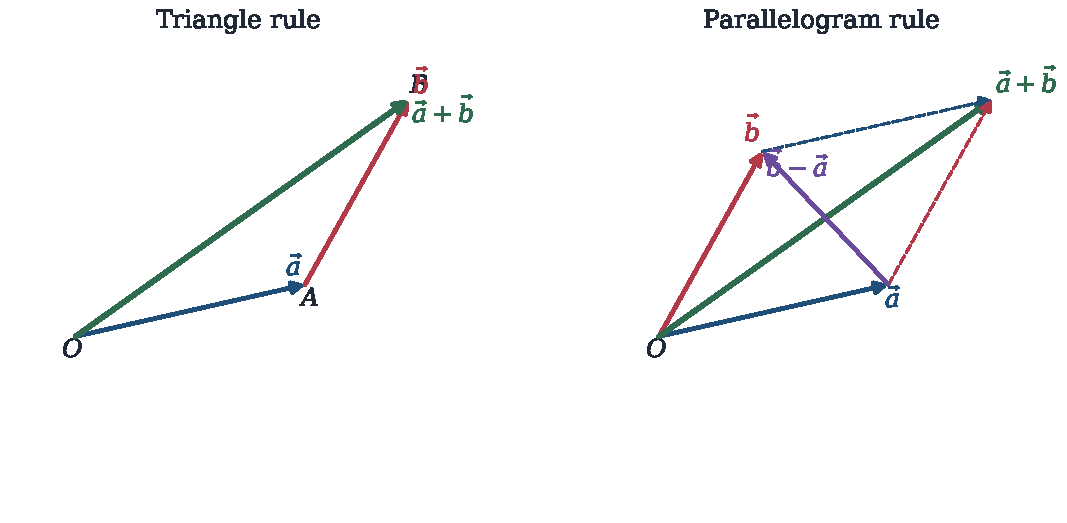
\includegraphics[width=0.95\textwidth]{figures/01_vector_addition.pdf}
\caption{Two equivalent constructions for the sum of two vectors. The difference
$\vec b-\vec a$ is the vector that must be added to $\vec a$ to obtain $\vec b$.}
\label{fig:vector-addition}
\end{figure}

\section{Vector algebra}

\subsection{Addition and subtraction}
Component by component:
\[
\vec{A}\pm\vec{B}=(A_x\pm B_x)\ihat+(A_y\pm B_y)\jhat+(A_z\pm B_z)\khat.
\]
Graphically, use the triangle or parallelogram rule
(\cref{fig:vector-addition}). Addition is commutative and associative.

\subsection{Scalar (dot) product}
\[
\vec{A}\cdot\vec{B}
=\norm{\vec{A}}\norm{\vec{B}}\cos\theta
=A_xB_x+A_yB_y+A_zB_z.
\]
The result is a scalar. In particular,
\[
\vec{A}\cdot\vec{B}=0\iff\vec{A}\perp\vec{B},
\qquad
\vec{A}\cdot\vec{A}=\norm{\vec{A}}^2.
\]
The projection of $\vec B$ onto the direction of $\vec A$ is
$B\cos\theta=(\vec A\cdot\vec B)/\norm{\vec A}$.

\begin{figure}[htbp]
\centering
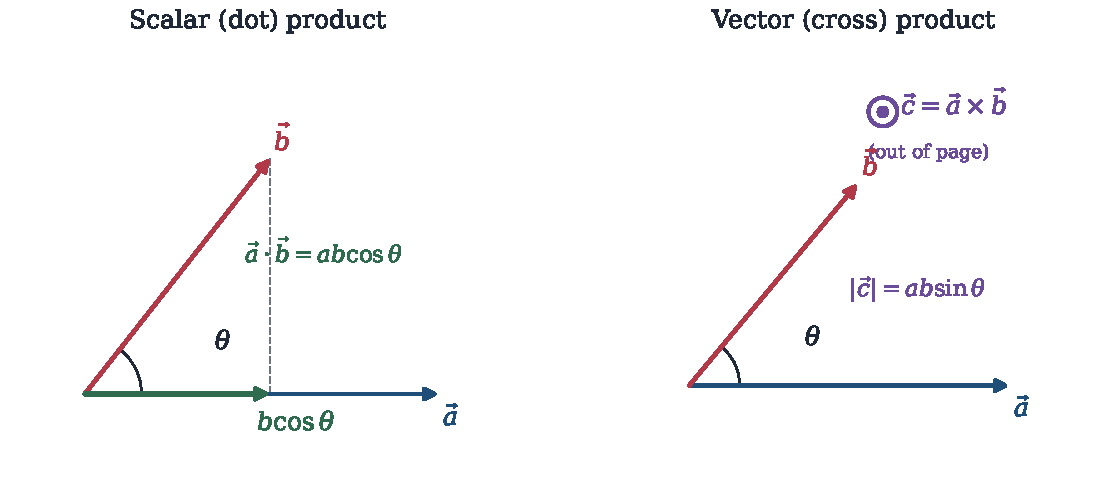
\includegraphics[width=0.95\textwidth]{figures/03_dot_cross.pdf}
\caption{The scalar product measures projection; the vector product measures the
area of the parallelogram and points along the right-hand normal.}
\label{fig:dot-cross}
\end{figure}

\subsection{Vector (cross) product}
\[
\vec{A}\times\vec{B}
=\begin{vmatrix}
\ihat & \jhat & \khat\\
A_x & A_y & A_z\\
B_x & B_y & B_z
\end{vmatrix},
\qquad
\norm{\vec{A}\times\vec{B}}
=\norm{\vec{A}}\norm{\vec{B}}\sin\theta.
\]
The result is a vector perpendicular to both $\vec A$ and $\vec B$, oriented by the
right-hand rule (\cref{fig:dot-cross}). The product is anti-commutative:
$\vec A\times\vec B=-(\vec B\times\vec A)$. Moreover,
\[
\vec{A}\times\vec{B}=\vzero\iff\vec{A}\parallel\vec{B}.
\]

\subsection{Triple products}
The scalar triple product gives the signed volume of the parallelepiped built on
the three vectors:
\[
\vec{A}\cdot(\vec{B}\times\vec{C})
=\begin{vmatrix}
A_x&A_y&A_z\\
B_x&B_y&B_z\\
C_x&C_y&C_z
\end{vmatrix}.
\]
The vector triple product satisfies
\[
\vec{A}\times(\vec{B}\times\vec{C})
=(\vec{A}\cdot\vec{C})\vec{B}-(\vec{A}\cdot\vec{B})\vec{C}.
\]

\section{Vector functions and their derivatives}

If a vector depends on time, $\vec{A}(t)=A_x(t)\ihat+A_y(t)\jhat+A_z(t)\khat$,
then
\[
\frac{\dd\vec{A}}{\dd t}
=\dot A_x\ihat+\dot A_y\jhat+\dot A_z\khat.
\]
The usual rules hold:
\[
\frac{\dd}{\dd t}(\vec A+\vec B)=\dot{\vec A}+\dot{\vec B},\qquad
\frac{\dd}{\dd t}(\vec A\cdot\vec B)
=\dot{\vec A}\cdot\vec B+\vec A\cdot\dot{\vec B},
\]
\[
\frac{\dd}{\dd t}(\vec A\times\vec B)
=\dot{\vec A}\times\vec B+\vec A\times\dot{\vec B}.
\]

\begin{keyidea}[Why derivatives matter]
Velocity is the time derivative of the position vector and acceleration is the
time derivative of velocity. Master the differentiation of vectors and kinematics
becomes bookkeeping.
\end{keyidea}

\section{Differential operators}

For a scalar field $f(x,y,z)$ and a vector field
$\vec{V}=V_x\ihat+V_y\jhat+V_z\khat$:

\begin{align*}
\grad f &= \frac{\partial f}{\partial x}\ihat
+\frac{\partial f}{\partial y}\jhat
+\frac{\partial f}{\partial z}\khat,\\[2pt]
\divg\vec V &= \frac{\partial V_x}{\partial x}
+\frac{\partial V_y}{\partial y}
+\frac{\partial V_z}{\partial z},\\[2pt]
\rot\vec V &=
\begin{vmatrix}
\ihat & \jhat & \khat\\[2pt]
\dfrac{\partial}{\partial x} & \dfrac{\partial}{\partial y} & \dfrac{\partial}{\partial z}\\[4pt]
V_x & V_y & V_z
\end{vmatrix},\\[2pt]
\Delta f &= \divg(\grad f)
=\frac{\partial^2f}{\partial x^2}
+\frac{\partial^2f}{\partial y^2}
+\frac{\partial^2f}{\partial z^2}.
\end{align*}

Two identities are used repeatedly:
\[
\rot(\grad f)=\vzero,\qquad \divg(\rot\vec V)=0.
\]
The first says that every gradient field is irrotational; it is the mathematical
basis of conservative forces in \cref{ch:energy}.

\begin{figure}[htbp]
\centering
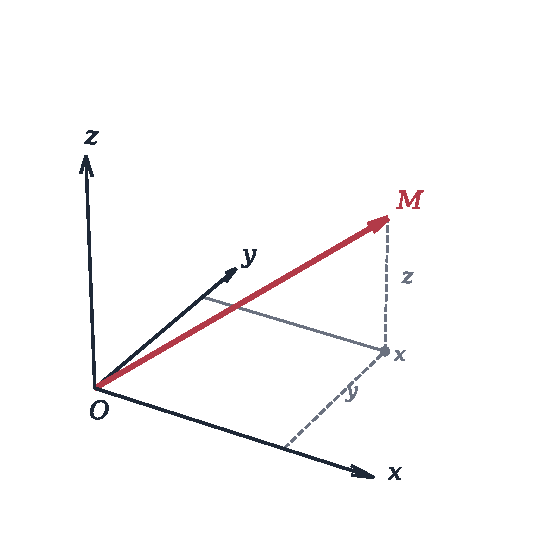
\includegraphics[width=0.72\textwidth]{figures/02_cartesian_3d.pdf}
\caption{The Cartesian components of the position vector $\vec{OM}$.}
\label{fig:cartesian}
\end{figure}

% ===========================================================================
\section{Worked examples}

\begin{worked}[Full vector algebra]
Let $\vec A=2\ihat-3\jhat+\khat$ and $\vec B=-\ihat+4\jhat-2\khat$. Compute
$\vec A+\vec B$, $\norm{\vec A}$, $\vec A\cdot\vec B$, the angle between them, and
$\vec A\times\vec B$.
\end{worked}

\begin{solution}{2.1}
\[
\vec A+\vec B=(2-1)\ihat+(-3+4)\jhat+(1-2)\khat
=\ihat+\jhat-\khat.
\]
\[
\norm{\vec A}=\sqrt{2^2+(-3)^2+1^2}=\sqrt{14}=3.74.
\]
\[
\vec A\cdot\vec B=(2)(-1)+(-3)(4)+(1)(-2)
=-2-12-2=-16.
\]
Since $\vec A\cdot\vec B=\norm{\vec A}\norm{\vec B}\cos\theta$ and
$\norm{\vec B}=\sqrt{1+16+4}=\sqrt{21}=4.58$,
\[
\cos\theta=\frac{-16}{\sqrt{14}\sqrt{21}}
=\frac{-16}{17.15}=-0.933,
\qquad
\theta=159^\circ.
\]
Finally,
\[
\vec A\times\vec B=
\begin{vmatrix}
\ihat&\jhat&\khat\\
2&-3&1\\
-1&4&-2
\end{vmatrix}
=(6-4)\ihat-(-4+1)\jhat+(8-3)\khat
=2\ihat+3\jhat+5\khat.
\]
Check: $(2,3,5)\cdot(2,-3,1)=4-9+5=0$ and
$(2,3,5)\cdot(-1,4,-2)=-2+12-10=0$.
\end{solution}

\begin{worked}[Gradient and conservative field]
For $f(x,y,z)=x^2y+yz^3$, compute $\grad f$ at $P(1,2,-1)$. Then find the force
field $\vec F=-\grad f$ and verify that $\rot\vec F=\vzero$.
\end{worked}

\begin{solution}{2.2}
\[
\frac{\partial f}{\partial x}=2xy,\qquad
\frac{\partial f}{\partial y}=x^2+z^3,\qquad
\frac{\partial f}{\partial z}=3yz^2.
\]
At $(1,2,-1)$:
\[
\grad f=(4)\ihat+(1-1)\jhat+(3\cdot2\cdot1)\khat
=4\ihat+6\khat.
\]
Thus $\vec F=-4\ihat-6\khat$ at $P$. Since $\vec F=-\grad f$ is a gradient
field, $\rot\vec F=-\rot(\grad f)=\vzero$ identically. Directly,
\[
\vec F=(-2xy,-x^2-z^3,-3yz^2),
\]
and each component of the curl cancels.
\end{solution}

% ===========================================================================
\section{Exercises and Step-by-Step Solutions}

\begin{exercise}{\warm\ Components and magnitude}
Let $\vec A=3\ihat+4\jhat$ and $\vec B=-2\ihat+5\jhat$. Find
$\vec A+\vec B$, $\vec A-\vec B$, $\norm{\vec A}$, $\norm{\vec B}$, and the unit
vectors $\vec u_A$ and $\vec u_B$.
\end{exercise}

\begin{tabletworkspace}[6.5cm]
\end{tabletworkspace}

\begin{solution}{2.1}
\[
\vec A+\vec B=(3-2)\ihat+(4+5)\jhat=\ihat+9\jhat,
\]
\[
\vec A-\vec B=(3+2)\ihat+(4-5)\jhat=5\ihat-\jhat.
\]
\[
\norm{\vec A}=\sqrt{9+16}=5,\qquad \norm{\vec B}=\sqrt{4+25}=\sqrt{29}=5.39.
\]
\[
\vec u_A=\frac{3}{5}\ihat+\frac{4}{5}\jhat,\qquad
\vec u_B=\frac{-2}{\sqrt{29}}\ihat+\frac{5}{\sqrt{29}}\jhat.
\]
\end{solution}

\begin{exercise}{\warm\ Dot product and angle}
For $\vec A=(1,2,3)$ and $\vec B=(4,-5,6)$, compute $\vec A\cdot\vec B$ and the
angle between the two vectors.
\end{exercise}

\begin{tabletworkspace}[6.5cm]
\end{tabletworkspace}

\begin{solution}{2.2}
\[
\vec A\cdot\vec B=4-10+18=12.
\]
\[
\norm{\vec A}=\sqrt{14}=3.742,\qquad \norm{\vec B}=\sqrt{77}=8.775.
\]
\[
\cos\theta=\frac{12}{(3.742)(8.775)}=0.3655,
\qquad \theta=68.6^\circ.
\]
\end{solution}

\begin{exercise}{\warm\ Cross product and area}
For $\vec A=(3,1,0)$ and $\vec B=(1,2,-1)$, compute $\vec A\times\vec B$ and the
area of the parallelogram spanned by the two vectors.
\end{exercise}

\begin{tabletworkspace}[6.5cm]
\end{tabletworkspace}

\begin{solution}{2.3}
\[
\vec A\times\vec B=
\begin{vmatrix}
\ihat&\jhat&\khat\\
3&1&0\\
1&2&-1
\end{vmatrix}
=(-1-0)\ihat-( -3-0)\jhat+(6-1)\khat
=-\ihat+3\jhat+5\khat.
\]
The area is
\[
\norm{\vec A\times\vec B}=\sqrt{1+9+25}=\sqrt{35}=5.92.
\]
\end{solution}

\begin{exercise}{\core\ Perpendicular and parallel conditions}
(a) Find $\lambda$ such that $\vec A=(2,\lambda,1)$ is perpendicular to
$\vec B=(3,-1,2)$. (b) Find $\mu$ such that $\vec C=(\mu,-1,2)$ is parallel to
$\vec B$.
\end{exercise}

\begin{tabletworkspace}[6.5cm]
\end{tabletworkspace}

\begin{solution}{2.4}
(a) Perpendicularity requires $\vec A\cdot\vec B=0$:
\[
(2)(3)+(\lambda)(-1)+(1)(2)=0
\implies 8-\lambda=0
\implies \lambda=8.
\]
(b) Parallelism requires $\vec C$ to be a multiple of $\vec B$. The second
component already matches, so the multiplier is $1$; hence $\mu=3$.
\end{solution}

\begin{exercise}{\core\ Scalar triple product}
For $\vec A=(1,0,2)$, $\vec B=(2,1,0)$, and $\vec C=(0,3,1)$, compute
$\vec A\cdot(\vec B\times\vec C)$ and the volume of the parallelepiped they
define.
\end{exercise}

\begin{tabletworkspace}[6.5cm]
\end{tabletworkspace}

\begin{solution}{2.5}
\[
\vec B\times\vec C=
\begin{vmatrix}
\ihat&\jhat&\khat\\
2&1&0\\
0&3&1
\end{vmatrix}
=\ihat-2\jhat+6\khat.
\]
\[
\vec A\cdot(\vec B\times\vec C)
=(1)(1)+(0)(-2)+(2)(6)=13.
\]
The volume is $\abs{13}=13$ cubic units.
\end{solution}

\begin{exercise}{\core\ Vector triple product}
Verify the identity
$\vec A\times(\vec B\times\vec C)=(\vec A\cdot\vec C)\vec B-(\vec A\cdot\vec B)\vec C$
for $\vec A=(1,2,0)$, $\vec B=(0,1,3)$, and $\vec C=(2,0,1)$.
\end{exercise}

\begin{tabletworkspace}[6.5cm]
\end{tabletworkspace}

\begin{solution}{2.6}
First,
\[
\vec B\times\vec C=
\begin{vmatrix}
\ihat&\jhat&\khat\\
0&1&3\\
2&0&1
\end{vmatrix}
=\ihat+6\jhat-2\khat.
\]
Then
\[
\vec A\times(\vec B\times\vec C)=
\begin{vmatrix}
\ihat&\jhat&\khat\\
1&2&0\\
1&6&-2
\end{vmatrix}
=(-4)\ihat-( -2)\jhat+(6-2)\khat
=-4\ihat+2\jhat+4\khat.
\]
On the other hand, $\vec A\cdot\vec C=2$ and $\vec A\cdot\vec B=2$, so
\[
2\vec B-2\vec C=(0,2,6)-(4,0,2)=(-4,2,4).
\]
The two results agree.
\end{solution}

\begin{exercise}{\core\ Differentiating a vector}
A particle has position $\vec r(t)=(3t^2,2t,t^3)$ (SI units). Find its velocity
and acceleration at $t=1.00\ \mathrm{s}$, and the magnitudes of both.
\end{exercise}

\begin{tabletworkspace}[6.5cm]
\end{tabletworkspace}

\begin{solution}{2.7}
\[
\vec v(t)=\dot{\vec r}=(6t,2,3t^2),\qquad
\vec a(t)=\ddot{\vec r}=(6,0,6t).
\]
At $t=1$:
\[
\vec v=(6,2,3)\ \mathrm{m\,s^{-1}},\qquad
\norm{\vec v}=\sqrt{36+4+9}=7.00\ \mathrm{m\,s^{-1}},
\]
\[
\vec a=(6,0,6)\ \mathrm{m\,s^{-2}},\qquad
\norm{\vec a}=\sqrt{36+36}=8.49\ \mathrm{m\,s^{-2}}.
\]
\end{solution}

\begin{exercise}{\core\ Gradient}
For $f(x,y,z)=x^2+y^2+z^2$, compute $\grad f$ at $P(1,2,2)$, its magnitude, and
the unit vector in the direction of steepest increase.
\end{exercise}

\begin{tabletworkspace}[6.5cm]
\end{tabletworkspace}

\begin{solution}{2.8}
\[
\grad f=(2x,2y,2z).
\]
At $P(1,2,2)$:
\[
\grad f=(2,4,4),\qquad \norm{\grad f}=\sqrt{4+16+16}=6.00.
\]
The direction of steepest increase is
\[
\vec u=\frac{1}{6}(2,4,4)=\left(\frac13,\frac23,\frac23\right).
\]
\end{solution}

\begin{exercise}{\mastery\ Divergence and curl}
For $\vec V=(x^2y,\,yz^2,\,xz)$, compute $\divg\vec V$ and $\rot\vec V$, and
verify explicitly that $\divg(\rot\vec V)=0$.
\end{exercise}

\begin{tabletworkspace}[6.5cm]
\end{tabletworkspace}

\begin{solution}{2.9}
\[
\divg\vec V=\frac{\partial}{\partial x}(x^2y)
+\frac{\partial}{\partial y}(yz^2)
+\frac{\partial}{\partial z}(xz)
=2xy+z^2+x.
\]
For the curl,
\[
\rot\vec V=
\left(
\frac{\partial V_z}{\partial y}-\frac{\partial V_y}{\partial z},
\frac{\partial V_x}{\partial z}-\frac{\partial V_z}{\partial x},
\frac{\partial V_y}{\partial x}-\frac{\partial V_x}{\partial y}
\right)
=(-2yz,\,-z,\,-x^2).
\]
Then
\[
\divg(\rot\vec V)
=\frac{\partial(-2yz)}{\partial x}
+\frac{\partial(-z)}{\partial y}
+\frac{\partial(-x^2)}{\partial z}
=0.
\]
\end{solution}

\begin{exercise}{\mastery\ Recovering a potential}
Show that
$\vec F=(y^2,\,2xy+z,\,y)$
is conservative, then find a scalar function $\varphi(x,y,z)$ such that
$\vec F=\grad\varphi$.
\end{exercise}

\begin{tabletworkspace}[6.5cm]
\end{tabletworkspace}

\begin{solution}{2.10}
Write $\vec F=(F_x,F_y,F_z)=(y^2,\,2xy+z,\,y)$. Compute
\[
\rot\vec F=
\left(
\frac{\partial F_z}{\partial y}-\frac{\partial F_y}{\partial z},
\frac{\partial F_x}{\partial z}-\frac{\partial F_z}{\partial x},
\frac{\partial F_y}{\partial x}-\frac{\partial F_x}{\partial y}
\right)
=(1-1,\,0-0,\,2y-2y)=\vzero.
\]
The field is irrotational, hence conservative. To find $\varphi$:
\[
\frac{\partial\varphi}{\partial x}=y^2
\implies \varphi=xy^2+g(y,z).
\]
Then
\[
\frac{\partial\varphi}{\partial y}=2xy+\frac{\partial g}{\partial y}=2xy+z
\implies \frac{\partial g}{\partial y}=z
\implies g=yz+h(z).
\]
Finally
\[
\frac{\partial\varphi}{\partial z}=y+h'(z)=y
\implies h'(z)=0.
\]
Thus
\[
\varphi(x,y,z)=xy^2+yz+C.
\]
\end{solution}



\part{Kinematics}

\chapter{The Language of Motion}
\label{ch:language}
\begin{chapterintro}
\textbf{You will learn to:} define a reference frame; write the position vector of
a particle; obtain velocity and acceleration by differentiation; eliminate time
to find a trajectory; and interpret motion graphically.
\end{chapterintro}

\section{Reference frame and position}

Motion is always described \emph{relative to a reference frame}. A frame consists
of an origin $O$, a set of axes, and a clock. The position of a material point
$M$ is the vector
\[
\vec{OM}(t)=\vec r(t)=x(t)\ihat+y(t)\jhat+z(t)\khat.
\]
The \textbf{trajectory} is the set of points actually visited. It is obtained by
eliminating the time $t$ from the three parametric equations $x(t),y(t),z(t)$.

A \textbf{material point} is a body whose size is negligible compared with the
distances involved. A train moving between two cities can be a point; a
gymnast rotating about the bar cannot.

\section{Velocity and acceleration}

The average velocity between $t$ and $t+\Delta t$ is
\[
\vec v_{\mathrm{av}}=\frac{\Delta\vec r}{\Delta t}
=\frac{\vec r(t+\Delta t)-\vec r(t)}{\Delta t}.
\]
The instantaneous velocity is the limit:
\[
\vec v(t)=\frac{\dd\vec r}{\dd t}
=\dot x\,\ihat+\dot y\,\jhat+\dot z\,\khat.
\]
The acceleration is the derivative of velocity:
\[
\vec a(t)=\frac{\dd\vec v}{\dd t}
=\frac{\dd^2\vec r}{\dd t^2}
=\ddot x\,\ihat+\ddot y\,\jhat+\ddot z\,\khat.
\]

\begin{keyidea}[Speed versus velocity]
Velocity is a vector. \textbf{Speed} is its magnitude,
$v=\norm{\vec v}=\sqrt{\dot x^2+\dot y^2+\dot z^2}$, and is never negative.
\end{keyidea}

\begin{figure}[htbp]
\centering
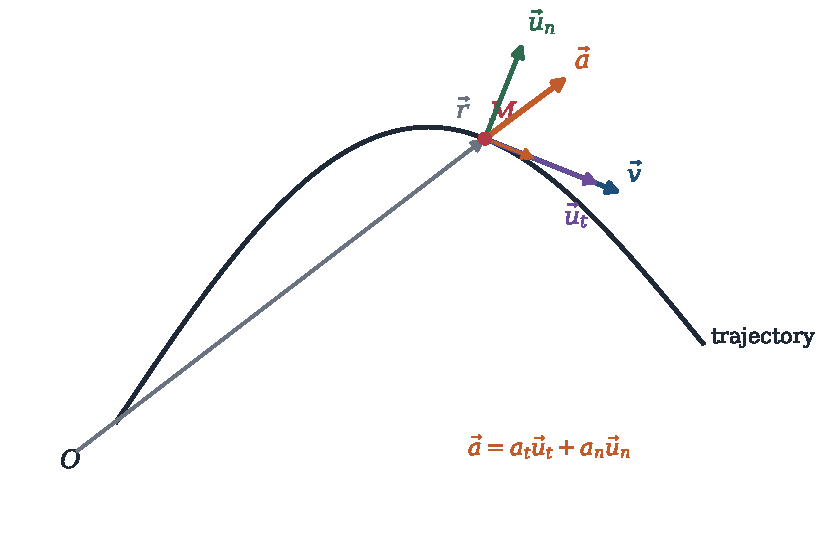
\includegraphics[width=0.88\textwidth]{figures/04_trajectory_frame.pdf}
\caption{At a point of a curved trajectory, the velocity is tangent to the path.
The acceleration generally has a tangential part (changing the speed) and a normal
part (changing the direction).}
\label{fig:trajectory-frame}
\end{figure}

\section{Graphical interpretation}

For one-dimensional motion along $x$:
\begin{itemize}[leftmargin=1.4em,itemsep=3pt]
  \item the slope of the $x$--$t$ graph is the velocity $v=\dd x/\dd t$;
  \item the slope of the $v$--$t$ graph is the acceleration $a=\dd v/\dd t$;
  \item the area under the $v$--$t$ graph is the displacement
        $\Delta x=\int v\,\dd t$;
  \item the area under the $a$--$t$ graph is the change in velocity
        $\Delta v=\int a\,\dd t$.
\end{itemize}

\begin{method}[From acceleration to position]
Given $a(t)$, integrate once to get $v(t)$ and again to get $x(t)$. At each
integration, use the initial conditions $v(0)$ and $x(0)$ to fix the constants.
\end{method}

% ===========================================================================
\section{Worked examples}

\begin{worked}[Position, velocity, acceleration, trajectory]
A particle has position
$\vec r(t)=2t\,\ihat+3t^2\,\jhat+\khat$ (SI units). Find its velocity and
acceleration at $t=1.00\ \mathrm{s}$, its speed, and the equation of its
trajectory.
\end{worked}

\begin{solution}{3.1}
Differentiate component by component:
\[
\vec v(t)=\dot{\vec r}=2\ihat+6t\jhat,\qquad
\vec a(t)=\ddot{\vec r}=6\jhat.
\]
At $t=1$:
\[
\vec v=2\ihat+6\jhat\ \mathrm{m\,s^{-1}},\quad
v=\sqrt{4+36}=6.32\ \mathrm{m\,s^{-1}},
\]
\[
\vec a=6\jhat\ \mathrm{m\,s^{-2}},\quad a=6.00\ \mathrm{m\,s^{-2}}.
\]
For the trajectory, $x=2t$ gives $t=x/2$. Then
\[
y=3t^2=3\left(\frac x2\right)^2=\frac{3x^2}{4},
\]
with $z=1$. The path is a parabola in the horizontal plane $z=1$.
\end{solution}

\begin{worked}[Average versus instantaneous velocity]
A particle moves along the $x$-axis with $x(t)=t^2-4t+3$ (SI units). Find the
average velocity between $t=0$ and $t=3.00\ \mathrm{s}$, and the instantaneous
velocity at $t=1.50\ \mathrm{s}$.
\end{worked}

\begin{solution}{3.2}
\[
x(0)=3,\qquad x(3)=9-12+3=0.
\]
\[
v_{\mathrm{av}}=\frac{x(3)-x(0)}{3-0}=\frac{0-3}{3}=-1.00\ \mathrm{m\,s^{-1}}.
\]
The instantaneous velocity is
\[
v(t)=\dot x=2t-4,
\qquad
v(1.50)=2(1.50)-4=-1.00\ \mathrm{m\,s^{-1}}.
\]
The two happen to be equal here, but they are conceptually different quantities.
\end{solution}

% ===========================================================================
\section{Exercises and Step-by-Step Solutions}

\begin{exercise}{\warm\ Straight-line kinematics}
A particle has position $\vec r(t)=4t\,\ihat+3t^2\,\jhat$ (SI units).
(a) Find $\vec v(t)$ and $\vec a(t)$.
(b) Find the speed at $t=1.00\ \mathrm{s}$.
(c) Find the Cartesian equation of the trajectory.
\end{exercise}

\begin{tabletworkspace}[6.5cm]
\end{tabletworkspace}

\begin{solution}{3.1}
(a)
\[
\vec v=(4,\,6t),\qquad \vec a=(0,\,6).
\]
(b) At $t=1$: $\vec v=(4,6)$, so
$v=\sqrt{16+36}=\sqrt{52}=7.21\ \mathrm{m\,s^{-1}}$.

(c) From $x=4t$, $t=x/4$. Then
\[
y=3\left(\frac x4\right)^2=\frac{3x^2}{16}.
\]
The trajectory is a parabola.
\end{solution}

\begin{exercise}{\warm\ One-dimensional motion}
The position of a particle on the $x$-axis is $x(t)=2t^3-3t^2+1$ (SI units).
(a) Find $v(t)$ and $a(t)$.
(b) Find the velocity and acceleration at $t=2.00\ \mathrm{s}$.
(c) At what times is the particle instantaneously at rest?
\end{exercise}

\begin{tabletworkspace}[6.5cm]
\end{tabletworkspace}

\begin{solution}{3.2}
(a)
\[
v(t)=6t^2-6t=6t(t-1),\qquad a(t)=12t-6.
\]
(b) At $t=2$:
\[
v=24-12=12.0\ \mathrm{m\,s^{-1}},\qquad a=24-6=18.0\ \mathrm{m\,s^{-2}}.
\]
(c) $v=0$ when $6t(t-1)=0$, i.e.\ $t=0$ and $t=1.00\ \mathrm{s}$.
\end{solution}

\begin{exercise}{\warm\ Average velocity}
A particle moves according to $x(t)=5t^2$ (SI units). Compute the average
velocity between $t=1.00\ \mathrm{s}$ and $t=3.00\ \mathrm{s}$, and compare it
with the instantaneous velocity at $t=2.00\ \mathrm{s}$.
\end{exercise}

\begin{tabletworkspace}[6.5cm]
\end{tabletworkspace}

\begin{solution}{3.3}
\[
x(1)=5,\qquad x(3)=45,
\]
\[
v_{\mathrm{av}}=\frac{45-5}{3-1}=20.0\ \mathrm{m\,s^{-1}}.
\]
The instantaneous velocity is $v(t)=10t$, so
$v(2)=20.0\ \mathrm{m\,s^{-1}}$. They are equal because $x\propto t^2$ is
quadratic; the average over a symmetric interval equals the instantaneous value
at the midpoint.
\end{solution}

\begin{exercise}{\core\ Uniform circular motion}
A particle moves in the $xy$-plane with
$\vec r(t)=R\cos(\omega t)\,\ihat+R\sin(\omega t)\,\jhat$, where $R$ and $\omega$
are constants.
(a) Show that the trajectory is a circle.
(b) Find $\vec v(t)$ and show that $\norm{\vec v}=R\omega$.
(c) Find $\vec a(t)$ and show that $\vec a=-\omega^2\vec r$.
\end{exercise}

\begin{tabletworkspace}[6.5cm]
\end{tabletworkspace}

\begin{solution}{3.4}
(a)
\[
x^2+y^2=R^2\cos^2(\omega t)+R^2\sin^2(\omega t)=R^2,
\]
a circle of radius $R$.

(b)
\[
\vec v=-R\omega\sin(\omega t)\,\ihat+R\omega\cos(\omega t)\,\jhat.
\]
\[
\norm{\vec v}=R\omega\sqrt{\sin^2+\cos^2}=R\omega.
\]

(c)
\[
\vec a=-R\omega^2\cos(\omega t)\,\ihat-R\omega^2\sin(\omega t)\,\jhat
=-\omega^2\vec r.
\]
Thus $\norm{\vec a}=R\omega^2$ and the acceleration points toward the centre.
\end{solution}

\begin{exercise}{\core\ Speed and unit tangent}
A particle has position
$\vec r(t)=2t\,\ihat+t^2\,\jhat+\frac{t^3}{3}\,\khat$ (SI units).
Find its velocity, speed, and unit tangent vector at $t=1.00\ \mathrm{s}$.
\end{exercise}

\begin{tabletworkspace}[6.5cm]
\end{tabletworkspace}

\begin{solution}{3.5}
\[
\vec v=(2,\,2t,\,t^2).
\]
At $t=1$:
\[
\vec v=(2,2,1),\qquad v=\sqrt{4+4+1}=3.00\ \mathrm{m\,s^{-1}}.
\]
The unit tangent vector is
\[
\utt=\frac{\vec v}{v}=\left(\frac23,\frac23,\frac13\right).
\]
\end{solution}

\begin{exercise}{\core\ Eliminating time}
A particle moves with $x(t)=2t$ and $y(t)=4t^2-1$ (SI units).
(a) Find the trajectory $y(x)$.
(b) Find $\vec v$ and $\vec a$ at $t=0.50\ \mathrm{s}$.
(c) Is the acceleration constant?
\end{exercise}

\begin{tabletworkspace}[6.5cm]
\end{tabletworkspace}

\begin{solution}{3.6}
(a) From $x=2t$, $t=x/2$, hence
\[
y=4\left(\frac x2\right)^2-1=x^2-1.
\]
This is a parabola opening upward.

(b) $\vec v=(2,8t)$ and $\vec a=(0,8)$. At $t=0.50$:
\[
\vec v=(2,4)\ \mathrm{m\,s^{-1}},\qquad
\norm{\vec v}=\sqrt{20}=4.47\ \mathrm{m\,s^{-1}},
\]
\[
\vec a=(0,8)\ \mathrm{m\,s^{-2}}.
\]
(c) Yes: $\vec a$ is independent of time, so the acceleration is constant.
\end{solution}

\begin{exercise}{\core\ Integrating acceleration}
A particle has acceleration $\vec a(t)=6t\,\ihat$ (SI units), initial velocity
$\vec v(0)=\ihat+2\jhat$, and initial position $\vec r(0)=\vzero$.
Find $\vec v(t)$, $\vec r(t)$, and the position at $t=2.00\ \mathrm{s}$.
\end{exercise}

\begin{tabletworkspace}[6.5cm]
\end{tabletworkspace}

\begin{solution}{3.7}
Integrating $\vec a=6t\,\ihat$:
\[
\vec v(t)=3t^2\ihat+\vec C.
\]
Using $\vec v(0)=\ihat+2\jhat$ gives $\vec C=\ihat+2\jhat$, so
\[
\vec v(t)=(3t^2+1)\ihat+2\jhat.
\]
Integrating again:
\[
\vec r(t)=(t^3+t)\ihat+2t\,\jhat+\vec D.
\]
With $\vec r(0)=\vzero$, $\vec D=\vzero$. Thus
\[
\vec r(t)=(t^3+t)\ihat+2t\,\jhat.
\]
At $t=2$: $\vec r=(8+2)\ihat+4\jhat=10\ihat+4\jhat$ (m).
\end{solution}

\begin{exercise}{\core\ From velocity to position}
A particle has velocity $\vec v(t)=3t^2\,\ihat+2t\,\jhat$ (SI units) and initial
position $\vec r(0)=\ihat$. Find $\vec r(t)$ and the speed at
$t=1.00\ \mathrm{s}$.
\end{exercise}

\begin{tabletworkspace}[6.5cm]
\end{tabletworkspace}

\begin{solution}{3.8}
Integrating $\vec v$:
\[
\vec r(t)=t^3\ihat+t^2\jhat+\vec C.
\]
With $\vec r(0)=\ihat$, $\vec C=\ihat$. Hence
\[
\vec r(t)=(t^3+1)\ihat+t^2\jhat.
\]
At $t=1$:
\[
\vec v=(3,2),\qquad v=\sqrt{9+4}=\sqrt{13}=3.61\ \mathrm{m\,s^{-1}}.
\]
\end{solution}

\begin{exercise}{\mastery\ Helical motion}
A particle moves on the helix
$\vec r(t)=a\cos(\omega t)\,\ihat+a\sin(\omega t)\,\jhat+bt\,\khat$.
(a) Show that its speed is constant.
(b) Find the magnitude of its acceleration.
(c) Describe the direction of the acceleration.
\end{exercise}

\begin{tabletworkspace}[6.5cm]
\end{tabletworkspace}

\begin{solution}{3.9}
(a)
\[
\vec v=-a\omega\sin(\omega t)\ihat+a\omega\cos(\omega t)\jhat+b\khat.
\]
\[
v^2=a^2\omega^2\sin^2+a^2\omega^2\cos^2+b^2
=a^2\omega^2+b^2=\text{const}.
\]
The speed is constant; the velocity direction changes.

(b)
\[
\vec a=-a\omega^2\cos(\omega t)\ihat-a\omega^2\sin(\omega t)\jhat,
\]
so
\[
\norm{\vec a}=a\omega^2.
\]
(c) The acceleration is horizontal and points toward the $z$-axis. It has no
vertical component: the helix is traversed at constant speed and constant
vertical velocity, while the horizontal projection is uniform circular motion.
\end{solution}

\begin{exercise}{\mastery\ Acceleration on a spiral path}
A particle moves in the $xy$-plane with
$\vec r(t)=R\cos(\alpha t^2)\,\ihat+R\sin(\alpha t^2)\,\jhat$, where $R$ and
$\alpha$ are constants.
(a) Find $\vec v(t)$ and $\vec a(t)$.
(b) Identify the tangential and normal components of $\vec a$.
(c) Verify that $a_n=v^2/R$.
\end{exercise}

\begin{tabletworkspace}[6.5cm]
\end{tabletworkspace}

\begin{solution}{3.10}
(a)
\[
\vec v=R(2\alpha t)\bigl[-\sin(\alpha t^2)\ihat+\cos(\alpha t^2)\jhat\bigr].
\]
Differentiating again,
\[
\vec a=R\bigl[-2\alpha\sin(\alpha t^2)-4\alpha^2t^2\cos(\alpha t^2)\bigr]\ihat
+R\bigl[2\alpha\cos(\alpha t^2)-4\alpha^2t^2\sin(\alpha t^2)\bigr]\jhat.
\]

(b) The unit tangent is
$\utt=-\sin(\alpha t^2)\ihat+\cos(\alpha t^2)\jhat$ and the unit normal is
$\un=-\cos(\alpha t^2)\ihat-\sin(\alpha t^2)\jhat$. Therefore
\[
\vec a=\underbrace{2R\alpha}_{a_t}\utt
+\underbrace{4R\alpha^2t^2}_{a_n}\un.
\]
The tangential acceleration is constant, $a_t=2R\alpha$; the normal acceleration
$a_n=4R\alpha^2t^2$ grows with time and points toward the centre (along $\un$).

(c) The speed is $v=2R\alpha t$, so
\[
\frac{v^2}{R}=\frac{4R^2\alpha^2t^2}{R}=4R\alpha^2t^2=\abs{a_n}.
\]
The relation $a_n=v^2/R$ holds, as it must for circular motion of radius $R$.
\end{solution}


\chapter{Rectilinear Motion}
\label{ch:rectilinear}
\begin{chapterintro}
\textbf{You will learn to:} solve uniform and uniformly accelerated rectilinear
motion; handle free fall; read motion graphs; and integrate a variable
acceleration.
\end{chapterintro}

\section{Uniform rectilinear motion}

When the acceleration is zero, the velocity is constant:
\[
a=0,\qquad v=v_0,\qquad x(t)=x_0+v_0t.
\]
The $x$--$t$ graph is a straight line of slope $v_0$.

\section{Uniformly accelerated rectilinear motion}

When $a$ is constant,
\[
v(t)=v_0+at,
\]
\[
x(t)=x_0+v_0t+\frac12at^2,
\]
and, eliminating $t$,
\[
v^2-v_0^2=2a(x-x_0).
\]
The last relation is useful when time is neither given nor asked for.

\begin{figure}[htbp]
\centering
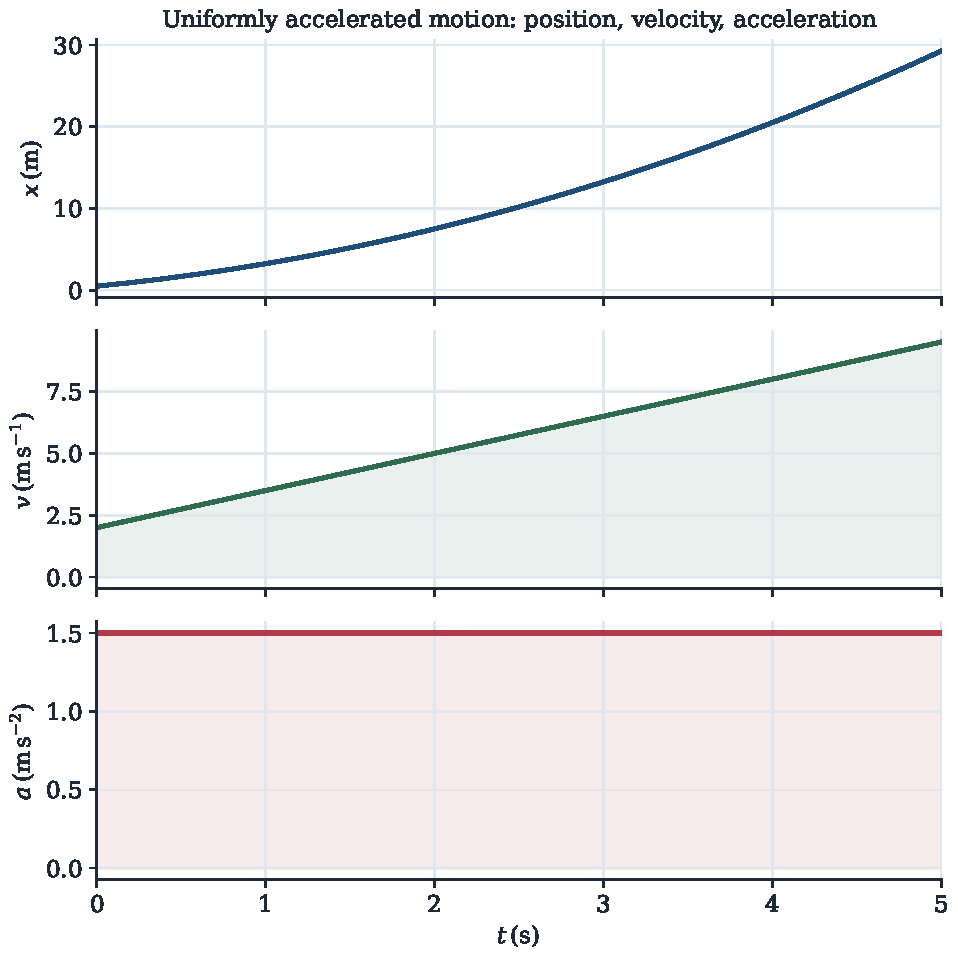
\includegraphics[width=0.78\textwidth]{figures/05_motion_graphs.pdf}
\caption{Uniformly accelerated motion with $x_0=0.5\ \mathrm{m}$,
$v_0=2.0\ \mathrm{m\,s^{-1}}$, and $a=1.5\ \mathrm{m\,s^{-2}}$. The slope of
$x(t)$ is $v(t)$; the slope of $v(t)$ is $a$; the area under $v(t)$ is the
displacement.}
\label{fig:motion-graphs}
\end{figure}

\section{Free fall}

Near the Earth's surface, neglecting air resistance, a body falls with constant
acceleration $\vec g$ directed downward. Taking the $y$-axis upward,
\[
a_y=-g,\qquad v_y=v_{0y}-gt,\qquad y=y_0+v_{0y}t-\frac12gt^2.
\]
With $g=9.81\ \mathrm{m\,s^{-2}}$.

\begin{warning}[Signs]
Choose a positive direction once and keep it for the whole problem. If upward is
positive, then $g$ enters as $-g$, a downward velocity is negative, and a
displacement below the starting point is negative.
\end{warning}

\section{Variable acceleration}

If $a$ is not constant, integrate:
\[
a(t)=\frac{\dd v}{\dd t}\implies v(t)=v(0)+\int_0^t a(t')\,\dd t',
\]
\[
v(t)=\frac{\dd x}{\dd t}\implies x(t)=x(0)+\int_0^t v(t')\,\dd t'.
\]
Two alternative forms are often useful:
\[
a=\frac{\dd v}{\dd t}=v\frac{\dd v}{\dd x}.
\]
The second form is the key to problems where the acceleration is given as a
function of position or speed.

\begin{method}[Choosing the right equation]
\begin{itemize}[leftmargin=1.3em,itemsep=2pt]
  \item Constant acceleration and time known: use $v=v_0+at$.
  \item Constant acceleration, time unknown: use $v^2=v_0^2+2a\Delta x$.
  \item Acceleration depends on $v$: separate variables in $\dd v/a(v)=\dd t$.
  \item Acceleration depends on $x$: use $v\,\dd v=a(x)\,\dd x$.
\end{itemize}
\end{method}

% ===========================================================================
\section{Worked examples}

\begin{worked}[Uniform acceleration]
A car accelerates uniformly from $10.0\ \mathrm{m\,s^{-1}}$ to
$30.0\ \mathrm{m\,s^{-1}}$ over a distance of $200\ \mathrm{m}$. Find its
acceleration and the time taken.
\end{worked}

\begin{solution}{4.1}
Use $v^2-v_0^2=2a\Delta x$:
\[
a=\frac{v^2-v_0^2}{2\Delta x}
=\frac{30.0^2-10.0^2}{2(200)}
=\frac{800}{400}=2.00\ \mathrm{m\,s^{-2}}.
\]
Then
\[
t=\frac{v-v_0}{a}=\frac{30.0-10.0}{2.00}=10.0\ \mathrm{s}.
\]
\end{solution}

\begin{worked}[Vertical throw]
A ball is thrown vertically upward from the ground with
$v_0=20.0\ \mathrm{m\,s^{-1}}$. Neglecting air resistance, find its maximum
height, the total time before it returns to the ground, and its velocity at
$t=3.00\ \mathrm{s}$.
\end{worked}

\begin{solution}{4.2}
Take upward as positive, so $a=-g=-9.81\ \mathrm{m\,s^{-2}}$.

At the highest point $v=0$:
\[
0=v_0^2-2gh
\implies
h=\frac{v_0^2}{2g}=\frac{400}{19.62}=20.4\ \mathrm{m}.
\]
The time to reach the top is $t_{\mathrm{up}}=v_0/g=2.04\ \mathrm{s}$; the total
time is twice this, $4.08\ \mathrm{s}$.

At $t=3.00\ \mathrm{s}$:
\[
v=20.0-9.81(3.00)=-9.43\ \mathrm{m\,s^{-1}}.
\]
The negative sign means the ball is moving downward.
\end{solution}

% ===========================================================================
\section{Exercises and Step-by-Step Solutions}

\begin{exercise}{\warm\ From zero to one hundred}
A car accelerates uniformly from rest to $100\ \mathrm{km\,h^{-1}}$ in
$8.00\ \mathrm{s}$. Find its acceleration and the distance covered.
\end{exercise}

\begin{tabletworkspace}[6.5cm]
\end{tabletworkspace}

\begin{solution}{4.1}
First convert:
\[
100\ \mathrm{km\,h^{-1}}=\frac{100}{3.6}=27.8\ \mathrm{m\,s^{-1}}.
\]
\[
a=\frac{v}{t}=\frac{27.8}{8.00}=3.47\ \mathrm{m\,s^{-2}}.
\]
\[
d=\frac12at^2=\frac12(3.47)(8.00)^2=111\ \mathrm{m}.
\]
Equivalently $d=v^2/(2a)=111\ \mathrm{m}$.
\end{solution}

\begin{exercise}{\warm\ Free fall}
A stone is dropped from rest from a height of $45.0\ \mathrm{m}$. Neglecting air
resistance, find the time to reach the ground and the impact speed.
\end{exercise}

\begin{tabletworkspace}[6.5cm]
\end{tabletworkspace}

\begin{solution}{4.2}
Taking downward as positive,
\[
h=\frac12gt^2
\implies
t=\sqrt{\frac{2h}{g}}=\sqrt{\frac{90.0}{9.81}}=3.03\ \mathrm{s}.
\]
\[
v=gt=9.81(3.03)=29.7\ \mathrm{m\,s^{-1}}.
\]
\end{solution}

\begin{exercise}{\warm\ Reading a position function}
A particle moves on the $x$-axis with $x(t)=3t^2-12t+7$ (SI units).
(a) Find $v(t)$ and $a(t)$.
(b) Find the time and value of the minimum position.
(c) Sketch $x(t)$ and describe the motion.
\end{exercise}

\begin{tabletworkspace}[6.5cm]
\end{tabletworkspace}

\begin{solution}{4.3}
(a)
\[
v(t)=6t-12,\qquad a(t)=6.
\]
(b) $v=0$ at $t=2.00\ \mathrm{s}$. Since $a>0$, this is a minimum:
\[
x(2)=3(4)-12(2)+7=-5.00\ \mathrm{m}.
\]
(c) For $t<2$ the particle moves in the negative $x$ direction; at $t=2$ it
stops instantaneously; for $t>2$ it moves in the positive direction with constant
acceleration $6\ \mathrm{m\,s^{-2}}$. The graph is an upward parabola with vertex
at $(2,-5)$.
\end{solution}

\begin{exercise}{\core\ Catching up}
Car A travels at a constant $20.0\ \mathrm{m\,s^{-1}}$. Car B starts from rest
from the same point $2.00\ \mathrm{s}$ later and accelerates uniformly at
$4.00\ \mathrm{m\,s^{-2}}$. When and where does B catch A? How fast is B moving
at that moment?
\end{exercise}

\begin{tabletworkspace}[6.5cm]
\end{tabletworkspace}

\begin{solution}{4.4}
Let $t$ be measured from the moment car A passes the reference point. Then
\[
x_A=20.0t,
\]
while car B starts at $t=2.00\ \mathrm{s}$:
\[
x_B=\frac12(4.00)(t-2.00)^2=2.00(t-2.00)^2.
\]
Set $x_A=x_B$:
\[
20.0t=2.00(t^2-4.00t+4.00)
\implies
2t^2-28t+8=0
\implies
t^2-14t+4=0.
\]
\[
t=\frac{14\pm\sqrt{196-16}}{2}=\frac{14\pm13.42}{2}.
\]
The physical solution is $t=13.7\ \mathrm{s}$ (the other root is before B starts).
Then
\[
x=20.0(13.7)=274\ \mathrm{m}.
\]
B's speed is
\[
v_B=4.00(13.7-2.00)=46.8\ \mathrm{m\,s^{-1}}.
\]
\end{solution}

\begin{exercise}{\core\ Vertical throw}
A ball is thrown vertically upward from the ground with
$v_0=15.0\ \mathrm{m\,s^{-1}}$. Find its maximum height, the time it returns to
the ground, and its velocity at $t=1.00\ \mathrm{s}$ and $t=2.50\ \mathrm{s}$.
\end{exercise}

\begin{tabletworkspace}[6.5cm]
\end{tabletworkspace}

\begin{solution}{4.5}
Upward positive, $a=-9.81\ \mathrm{m\,s^{-2}}$.
\[
h=\frac{v_0^2}{2g}=\frac{225}{19.62}=11.5\ \mathrm{m}.
\]
\[
t_{\mathrm{return}}=\frac{2v_0}{g}=\frac{30.0}{9.81}=3.06\ \mathrm{s}.
\]
At $t=1.00$:
\[
v=15.0-9.81=5.19\ \mathrm{m\,s^{-1}}.
\]
At $t=2.50$:
\[
v=15.0-9.81(2.50)=15.0-24.5=-9.53\ \mathrm{m\,s^{-1}}.
\]
\end{solution}

\begin{exercise}{\core\ Braking distance}
A train travelling at $30.0\ \mathrm{m\,s^{-1}}$ brakes uniformly and stops in
$500\ \mathrm{m}$. Find the deceleration and the stopping time.
\end{exercise}

\begin{tabletworkspace}[6.5cm]
\end{tabletworkspace}

\begin{solution}{4.6}
With $v=0$ and $v_0=30.0\ \mathrm{m\,s^{-1}}$,
\[
a=\frac{0-v_0^2}{2d}=-\frac{900}{1000}=-0.900\ \mathrm{m\,s^{-2}}.
\]
The deceleration magnitude is $0.900\ \mathrm{m\,s^{-2}}$.
\[
t=\frac{v-v_0}{a}=\frac{-30.0}{-0.900}=33.3\ \mathrm{s}.
\]
\end{solution}

\begin{exercise}{\core\ Velocity graph}
A particle moves along a straight line. Its velocity is
$4.00\ \mathrm{m\,s^{-1}}$ from $t=0$ to $t=3.00\ \mathrm{s}$, then decreases
linearly to zero at $t=7.00\ \mathrm{s}$.
(a) Draw the $v$--$t$ graph.
(b) Find the total displacement.
(c) Find the acceleration during the second phase.
\end{exercise}

\begin{tabletworkspace}[6.5cm]
\end{tabletworkspace}

\begin{solution}{4.7}
(a) The graph is horizontal at $4.00\ \mathrm{m\,s^{-1}}$ from $0$ to $3\ \mathrm{s}$,
then a straight line down to zero at $7\ \mathrm{s}$.

(b) The area is a rectangle plus a triangle:
\[
\Delta x=(3.00)(4.00)+\frac12(4.00)(4.00)=12.0+8.00=20.0\ \mathrm{m}.
\]

(c) During $3<t<7$,
\[
a=\frac{0-4.00}{7.00-3.00}=-1.00\ \mathrm{m\,s^{-2}}.
\]
\end{solution}

\begin{exercise}{\core\ Time-dependent acceleration}
A particle starts with $v(0)=1.00\ \mathrm{m\,s^{-1}}$ and $x(0)=0$, and has
acceleration $a(t)=2t\ \mathrm{m\,s^{-2}}$. Find $v(t)$, $x(t)$, and the position
at $t=2.00\ \mathrm{s}$.
\end{exercise}

\begin{tabletworkspace}[6.5cm]
\end{tabletworkspace}

\begin{solution}{4.8}
Integrating $a=2t$:
\[
v(t)=t^2+C_1.
\]
With $v(0)=1.00$, $C_1=1.00$, so $v(t)=t^2+1.00$.

Integrating again:
\[
x(t)=\frac{t^3}{3}+t+C_2.
\]
With $x(0)=0$, $C_2=0$. Thus
\[
x(t)=\frac{t^3}{3}+t.
\]
At $t=2.00$:
\[
x=\frac{8.00}{3}+2.00=4.67\ \mathrm{m}.
\]
\end{solution}

\begin{exercise}{\mastery\ Linear drag}
A particle moves on a straight line with acceleration $a=-kv$, where $k>0$ is a
constant. At $t=0$, $v=v_0$ and $x=0$.
(a) Find $v(t)$.
(b) Find $x(t)$.
(c) Show that the particle travels a finite maximum distance even though it never
stops in finite time.
\end{exercise}

\begin{tabletworkspace}[6.5cm]
\end{tabletworkspace}

\begin{solution}{4.9}
(a) Separate variables:
\[
\frac{\dd v}{\dd t}=-kv
\implies
\frac{\dd v}{v}=-k\,\dd t.
\]
Integrating from $0$ to $t$:
\[
\ln\frac{v}{v_0}=-kt
\implies
v(t)=v_0e^{-kt}.
\]

(b)
\[
x(t)=\int_0^t v_0e^{-kt'}\,\dd t'
=\frac{v_0}{k}\left(1-e^{-kt}\right).
\]

(c) As $t\to\infty$, $x\to v_0/k$, a finite limit. But $v=v_0e^{-kt}$ is never
exactly zero for any finite $t$. The particle asymptotically approaches the
position $x=v_0/k$ without ever reaching it in finite time.
\end{solution}

\begin{exercise}{\mastery\ Dropped and thrown}
A ball is dropped from rest from height $h$ at $t=0$. At the same instant, a
second ball is thrown vertically upward from the ground with speed $v_0$.
(a) Find the time at which the two balls meet.
(b) Find the height at which they meet.
(c) For $h=15.0\ \mathrm{m}$ and $v_0=10.0\ \mathrm{m\,s^{-1}}$, compute the
meeting time and height.
\end{exercise}

\begin{tabletworkspace}[6.5cm]
\end{tabletworkspace}

\begin{solution}{4.10}
Take upward as positive, with the ground at $y=0$. Then
\[
y_A=h-\frac12gt^2,\qquad
y_B=v_0t-\frac12gt^2.
\]
(a) Setting $y_A=y_B$:
\[
h-\frac12gt^2=v_0t-\frac12gt^2
\implies
t=\frac{h}{v_0}.
\]
(b) Substituting back,
\[
y=h-\frac12g\left(\frac{h}{v_0}\right)^2
=h-\frac{gh^2}{2v_0^2}.
\]
(c) For $h=15.0\ \mathrm{m}$ and $v_0=10.0\ \mathrm{m\,s^{-1}}$:
\[
t=\frac{15.0}{10.0}=1.50\ \mathrm{s},
\]
\[
y=15.0-\frac{9.81(15.0)^2}{2(10.0)^2}
=15.0-\frac{2207}{200}=15.0-11.0=3.96\ \mathrm{m}.
\]
\end{solution}


\chapter{Motion in a Plane: Projectiles and Circles}
\label{ch:plane}
\begin{chapterintro}
\textbf{You will learn to:} analyse projectile motion with constant acceleration;
compute range, maximum height, and time of flight; describe circular motion with
angular velocity and centripetal acceleration; and handle non-uniform circular
motion.
\end{chapterintro}

\section{Projectile motion}

Take the $y$-axis vertical and neglect air resistance. The only acceleration is
\[
a_x=0,\qquad a_y=-g.
\]
With initial speed $v_0$ at angle $\alpha$ above the horizontal:
\[
x(t)=(v_0\cos\alpha)t,\qquad
y(t)=(v_0\sin\alpha)t-\frac12gt^2.
\]
Eliminating $t$,
\[
y(x)=x\tan\alpha-\frac{gx^2}{2v_0^2\cos^2\alpha}.
\]
The trajectory is a parabola.

For a projectile launched and landing at the same height:
\[
T=\frac{2v_0\sin\alpha}{g},
\qquad
R=\frac{v_0^2\sin2\alpha}{g},
\qquad
H=\frac{v_0^2\sin^2\alpha}{2g}.
\]
The range is maximum at $\alpha=45^\circ$, where $R_{\max}=v_0^2/g$.

\begin{figure}[htbp]
\centering
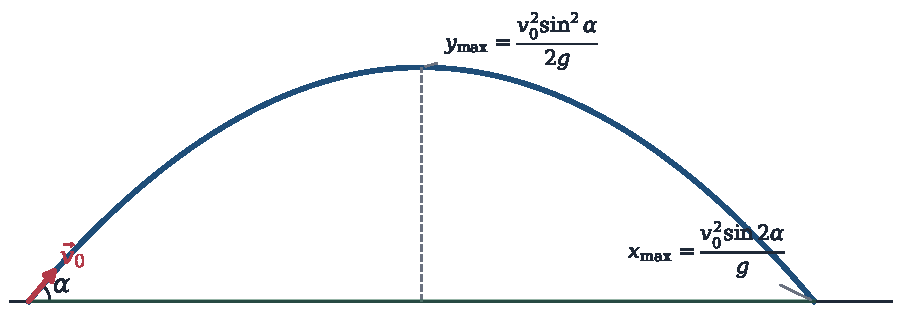
\includegraphics[width=0.9\textwidth]{figures/06_projectile.pdf}
\caption{Projectile motion: the velocity is tangent to the parabola, while the
acceleration is always vertically downward.}
\label{fig:projectile}
\end{figure}

\begin{warning}[Two frequent mistakes]
The horizontal velocity never changes (no air resistance), and the vertical
acceleration is $g$ even at the highest point. ``$a=0$ at the top'' is false:
only $v_y=0$ there.
\end{warning}

\section{Circular motion}

For a particle moving on a circle of radius $R$, let $\theta(t)$ be its angular
position. Define
\[
\omega=\dot\theta\quad(\mathrm{rad\,s^{-1}}),\qquad
\alpha=\dot\omega=\ddot\theta\quad(\mathrm{rad\,s^{-2}}).
\]
Then
\[
v=R\omega,\qquad
a_t=R\alpha,\qquad
a_n=\frac{v^2}{R}=R\omega^2.
\]
The tangential acceleration $a_t$ changes the speed; the normal (centripetal)
acceleration $a_n$ changes the direction and always points toward the centre.
The total acceleration has magnitude
\[
a=\sqrt{a_t^2+a_n^2}.
\]
The period of uniform circular motion is $T=2\pi/\omega$.

\begin{figure}[htbp]
\centering
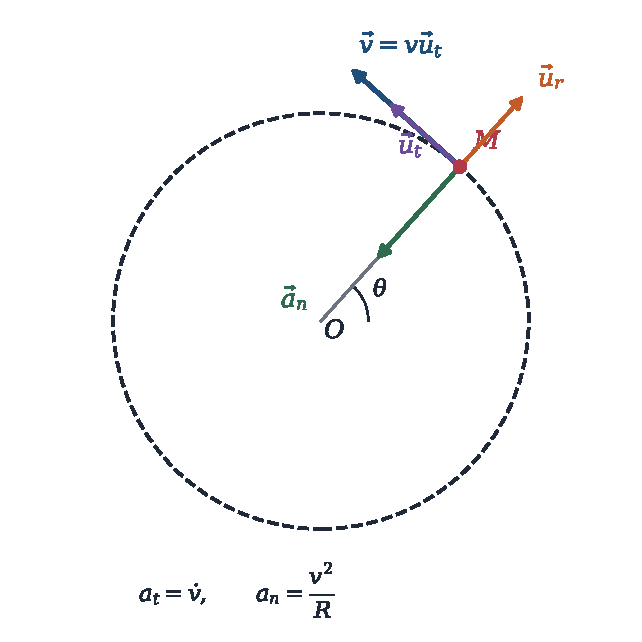
\includegraphics[width=0.68\textwidth]{figures/07_circular_motion.pdf}
\caption{Circular motion. The velocity is tangential; the centripetal
acceleration points toward the centre.}
\label{fig:circular}
\end{figure}

\begin{keyidea}[Intrinsic decomposition]
For any curved path, with $\utt$ the unit tangent and $\un$ the unit normal
pointing toward the centre of curvature,
\[
\vec a=\frac{\dd v}{\dd t}\utt+\frac{v^2}{R}\un.
\]
For a circle, $R$ is constant; for a general curve, $R$ is the local radius of
curvature.
\end{keyidea}

% ===========================================================================
\section{Worked examples}

\begin{worked}[Full projectile analysis]
A projectile is launched from the ground with $v_0=25.0\ \mathrm{m\,s^{-1}}$ at
$\alpha=40.0^\circ$. Find the time of flight, the range, the maximum height, and
the velocity at $t=1.50\ \mathrm{s}$.
\end{worked}

\begin{solution}{5.1}
\[
v_{0x}=25.0\cos40.0^\circ=19.2\ \mathrm{m\,s^{-1}},\qquad
v_{0y}=25.0\sin40.0^\circ=16.1\ \mathrm{m\,s^{-1}}.
\]
Time of flight:
\[
T=\frac{2v_{0y}}{g}=\frac{32.1}{9.81}=3.28\ \mathrm{s}.
\]
Range:
\[
R=v_{0x}T=(19.2)(3.28)=62.9\ \mathrm{m},
\]
or directly $R=v_0^2\sin80^\circ/g=62.7\ \mathrm{m}$.

Maximum height:
\[
H=\frac{v_{0y}^2}{2g}=\frac{258}{19.62}=13.2\ \mathrm{m}.
\]
At $t=1.50\ \mathrm{s}$:
\[
v_x=19.2\ \mathrm{m\,s^{-1}},\qquad
v_y=16.1-9.81(1.50)=1.36\ \mathrm{m\,s^{-1}},
\]
\[
v=\sqrt{19.2^2+1.36^2}=19.2\ \mathrm{m\,s^{-1}}.
\]
The projectile is still rising slightly.
\end{solution}

\begin{worked}[Non-uniform circular motion]
A particle moves on a circle of radius $R=0.500\ \mathrm{m}$ with angular
position $\theta(t)=2t^2$ (rad). At $t=1.00\ \mathrm{s}$, find the angular
velocity, angular acceleration, speed, tangential and normal accelerations, and
the total acceleration.
\end{worked}

\begin{solution}{5.2}
\[
\omega=\dot\theta=4t,\qquad \alpha=\dot\omega=4.
\]
At $t=1$: $\omega=4.00\ \mathrm{rad\,s^{-1}}$, $\alpha=4.00\ \mathrm{rad\,s^{-2}}$.

\[
v=R\omega=0.500(4.00)=2.00\ \mathrm{m\,s^{-1}},
\]
\[
a_t=R\alpha=0.500(4.00)=2.00\ \mathrm{m\,s^{-2}},
\]
\[
a_n=R\omega^2=0.500(16.0)=8.00\ \mathrm{m\,s^{-2}}.
\]
\[
a=\sqrt{2.00^2+8.00^2}=\sqrt{68.0}=8.25\ \mathrm{m\,s^{-2}}.
\]
\end{solution}

% ===========================================================================
\section{Exercises and Step-by-Step Solutions}

\begin{exercise}{\warm\ Basic projectile}
A ball is launched from the ground with $v_0=20.0\ \mathrm{m\,s^{-1}}$ at
$30.0^\circ$ above the horizontal. Find the time of flight, the range, and the
maximum height.
\end{exercise}

\begin{tabletworkspace}[6.5cm]
\end{tabletworkspace}

\begin{solution}{5.1}
\[
v_{0x}=20.0\cos30.0^\circ=17.3\ \mathrm{m\,s^{-1}},\qquad
v_{0y}=20.0\sin30.0^\circ=10.0\ \mathrm{m\,s^{-1}}.
\]
\[
T=\frac{2v_{0y}}{g}=\frac{20.0}{9.81}=2.04\ \mathrm{s}.
\]
\[
R=v_{0x}T=(17.3)(2.04)=35.3\ \mathrm{m}.
\]
\[
H=\frac{v_{0y}^2}{2g}=\frac{100}{19.62}=5.10\ \mathrm{m}.
\]
\end{solution}

\begin{exercise}{\warm\ Horizontal launch}
A ball is thrown horizontally from a cliff of height $20.0\ \mathrm{m}$ with
speed $15.0\ \mathrm{m\,s^{-1}}$. Find the time to reach the ground, the
horizontal distance travelled, and the impact speed.
\end{exercise}

\begin{tabletworkspace}[6.5cm]
\end{tabletworkspace}

\begin{solution}{5.2}
Vertical motion (downward positive):
\[
h=\frac12gt^2
\implies
t=\sqrt{\frac{2(20.0)}{9.81}}=2.02\ \mathrm{s}.
\]
Horizontal distance:
\[
x=v_0t=15.0(2.02)=30.3\ \mathrm{m}.
\]
Impact velocity:
\[
v_x=15.0,\qquad v_y=gt=19.8\ \mathrm{m\,s^{-1}},
\]
\[
v=\sqrt{15.0^2+19.8^2}=24.9\ \mathrm{m\,s^{-1}}.
\]
\end{solution}

\begin{exercise}{\warm\ Uniform circular motion}
A point moves on a circle of radius $2.00\ \mathrm{m}$ with period
$0.500\ \mathrm{s}$. Find its angular velocity, speed, and centripetal
acceleration.
\end{exercise}

\begin{tabletworkspace}[6.5cm]
\end{tabletworkspace}

\begin{solution}{5.3}
\[
\omega=\frac{2\pi}{T}=\frac{2\pi}{0.500}=12.6\ \mathrm{rad\,s^{-1}}.
\]
\[
v=R\omega=2.00(12.6)=25.1\ \mathrm{m\,s^{-1}}.
\]
\[
a_n=\frac{v^2}{R}=\frac{631}{2.00}=316\ \mathrm{m\,s^{-2}}.
\]
\end{solution}

\begin{exercise}{\core\ Range and maximum height}
A projectile launched at $45.0^\circ$ has a range of $100\ \mathrm{m}$. Find its
initial speed, maximum height, and time of flight.
\end{exercise}

\begin{tabletworkspace}[6.5cm]
\end{tabletworkspace}

\begin{solution}{5.4}
For $\alpha=45^\circ$, $\sin2\alpha=1$, so
\[
R=\frac{v_0^2}{g}
\implies
v_0=\sqrt{gR}=\sqrt{9.81(100)}=31.3\ \mathrm{m\,s^{-1}}.
\]
\[
H=\frac{v_0^2\sin^245^\circ}{2g}
=\frac{gR(1/2)}{2g}=\frac R4=25.0\ \mathrm{m}.
\]
\[
T=\frac{2v_0\sin45^\circ}{g}
=\frac{2(31.3)(0.707)}{9.81}=4.51\ \mathrm{s}.
\]
\end{solution}

\begin{exercise}{\core\ Clearing a wall}
A projectile is launched with $v_0=30.0\ \mathrm{m\,s^{-1}}$ at $50.0^\circ$.
A wall stands $60.0\ \mathrm{m}$ away. Does the projectile clear a wall of height
$10.0\ \mathrm{m}$? Find its height and velocity when it reaches the wall.
\end{exercise}

\begin{tabletworkspace}[6.5cm]
\end{tabletworkspace}

\begin{solution}{5.5}
\[
v_x=30.0\cos50.0^\circ=19.3\ \mathrm{m\,s^{-1}},\qquad
v_{0y}=30.0\sin50.0^\circ=23.0\ \mathrm{m\,s^{-1}}.
\]
Time to reach the wall:
\[
t=\frac{x}{v_x}=\frac{60.0}{19.3}=3.11\ \mathrm{s}.
\]
Height at that time:
\[
y=23.0(3.11)-\frac12(9.81)(3.11)^2
=71.5-47.4=24.1\ \mathrm{m}.
\]
This is well above $10.0\ \mathrm{m}$, so the projectile clears the wall.

Velocity at the wall:
\[
v_x=19.3,\qquad v_y=23.0-9.81(3.11)=-7.51\ \mathrm{m\,s^{-1}},
\]
\[
v=\sqrt{19.3^2+7.51^2}=20.7\ \mathrm{m\,s^{-1}},
\]
directed $21.3^\circ$ below the horizontal (the projectile is descending).
\end{solution}

\begin{exercise}{\core\ Speed at the top}
A projectile is launched at angle $\theta$ above the horizontal. At the highest
point its speed is exactly half its initial speed. Find $\theta$.
\end{exercise}

\begin{tabletworkspace}[6.5cm]
\end{tabletworkspace}

\begin{solution}{5.6}
At the highest point $v_y=0$, so the speed is $v_x=v_0\cos\theta$. The condition
$v=v_0/2$ gives
\[
v_0\cos\theta=\frac{v_0}{2}
\implies
\cos\theta=\frac12
\implies
\theta=60.0^\circ.
\]
\end{solution}

\begin{exercise}{\core\ Two angles, one range}
A projectile has initial speed $30.0\ \mathrm{m\,s^{-1}}$ and must reach a range
of $80.0\ \mathrm{m}$. Find the two possible launch angles and the corresponding
times of flight.
\end{exercise}

\begin{tabletworkspace}[6.5cm]
\end{tabletworkspace}

\begin{solution}{5.7}
\[
R=\frac{v_0^2\sin2\theta}{g}
\implies
\sin2\theta=\frac{gR}{v_0^2}
=\frac{9.81(80.0)}{(30.0)^2}=0.872.
\]
Thus
\[
2\theta=60.7^\circ\ \text{or}\ 119.3^\circ,
\]
so
\[
\theta_1=30.4^\circ,\qquad \theta_2=59.6^\circ.
\]
The times of flight are
\[
T_1=\frac{2(30.0)\sin30.4^\circ}{9.81}=3.10\ \mathrm{s},
\]
\[
T_2=\frac{2(30.0)\sin59.6^\circ}{9.81}=5.28\ \mathrm{s}.
\]
The lower angle gives the shorter flight and the smaller maximum height.
\end{solution}

\begin{exercise}{\core\ Angular kinematics}
A particle moves on a circle of radius $R=0.500\ \mathrm{m}$ with angular
position $\theta(t)=2t^2$ rad. At $t=1.00\ \mathrm{s}$, find $\omega$, $\alpha$,
$v$, $a_t$, $a_n$, and the total acceleration.
\end{exercise}

\begin{tabletworkspace}[6.5cm]
\end{tabletworkspace}

\begin{solution}{5.8}
\[
\omega=\dot\theta=4t,\qquad \alpha=\dot\omega=4.
\]
At $t=1.00\ \mathrm{s}$:
\[
\omega=4.00\ \mathrm{rad\,s^{-1}},\qquad
\alpha=4.00\ \mathrm{rad\,s^{-2}}.
\]
\[
v=R\omega=0.500(4.00)=2.00\ \mathrm{m\,s^{-1}},
\]
\[
a_t=R\alpha=0.500(4.00)=2.00\ \mathrm{m\,s^{-2}},
\]
\[
a_n=R\omega^2=0.500(16.0)=8.00\ \mathrm{m\,s^{-2}}.
\]
\[
a=\sqrt{a_t^2+a_n^2}=\sqrt{4.00+64.0}=8.25\ \mathrm{m\,s^{-2}}.
\]
\end{solution}

\begin{exercise}{\mastery\ Deriving the range formula}
Starting from $x=v_0\cos\alpha\,t$ and
$y=v_0\sin\alpha\,t-\frac12gt^2$, derive
\[
y=x\tan\alpha-\frac{gx^2}{2v_0^2\cos^2\alpha},
\]
then show that for equal launch and landing heights the range is
$R=v_0^2\sin2\alpha/g$. Deduce that the maximum range occurs at $45^\circ$ and
that complementary angles give the same range.
\end{exercise}

\begin{tabletworkspace}[6.5cm]
\end{tabletworkspace}

\begin{solution}{5.9}
From $x=v_0\cos\alpha\,t$,
\[
t=\frac{x}{v_0\cos\alpha}.
\]
Substituting into $y$:
\[
y=v_0\sin\alpha\frac{x}{v_0\cos\alpha}
-\frac12g\frac{x^2}{v_0^2\cos^2\alpha}
=x\tan\alpha-\frac{gx^2}{2v_0^2\cos^2\alpha}.
\]
At landing, $y=0$ and $x=R$:
\[
R\tan\alpha=\frac{gR^2}{2v_0^2\cos^2\alpha}.
\]
For $R\ne0$,
\[
R=\frac{2v_0^2\sin\alpha\cos\alpha}{g}
=\frac{v_0^2\sin2\alpha}{g}.
\]
This is maximum when $\sin2\alpha=1$, i.e.\ $2\alpha=90^\circ$ and
$\alpha=45^\circ$, giving $R_{\max}=v_0^2/g$. Since
$\sin(180^\circ-2\alpha)=\sin2\alpha$, the angles $\alpha$ and
$90^\circ-\alpha$ give the same range.
\end{solution}

\begin{exercise}{\mastery\ Hitting a target}
A projectile is launched from the origin with speed
$v_0=25.0\ \mathrm{m\,s^{-1}}$ and must pass through the point
$(x,y)=(30.0,10.0)\ \mathrm{m}$. Using $u=\tan\alpha$, show that
\[
\frac{gx^2}{2v_0^2}u^2-xu+\left(y+\frac{gx^2}{2v_0^2}\right)=0,
\]
and find the two possible launch angles.
\end{exercise}

\begin{tabletworkspace}[6.5cm]
\end{tabletworkspace}

\begin{solution}{5.10}
With $u=\tan\alpha$ and
$\cos^2\alpha=1/(1+u^2)$,
\[
y=xu-\frac{gx^2}{2v_0^2}(1+u^2).
\]
Rearranging,
\[
\frac{gx^2}{2v_0^2}u^2-xu+\left(y+\frac{gx^2}{2v_0^2}\right)=0.
\]
For $x=30.0\ \mathrm{m}$, $y=10.0\ \mathrm{m}$, $v_0=25.0\ \mathrm{m\,s^{-1}}$:
\[
A=\frac{9.81(30.0)^2}{2(25.0)^2}=7.063,
\]
so
\[
7.063u^2-30.0u+17.063=0.
\]
\[
u=\frac{30.0\pm\sqrt{900-4(7.063)(17.063)}}{2(7.063)}
=\frac{30.0\pm20.44}{14.126}.
\]
Thus
\[
u_1=3.57\implies\alpha_1=74.4^\circ,\qquad
u_2=0.677\implies\alpha_2=34.1^\circ.
\]
Both trajectories pass through the target; the low-angle shot arrives sooner.
\end{solution}


\chapter{Curvilinear Coordinates}
\label{ch:coordinates}
\begin{chapterintro}
\textbf{You will learn to:} express position, velocity, and acceleration in polar,
cylindrical, and spherical coordinates; differentiate the moving unit vectors; and
recognise the centripetal and Coriolis-like terms that appear in curvilinear
coordinates.
\end{chapterintro}

\section{Polar coordinates}

In the plane, a point $M$ is located by its distance $r$ from the origin and the
angle $\theta$ measured from the $x$-axis. The associated unit vectors are
$\ur$ (radial, pointing away from $O$) and $\ut$ (perpendicular to $\ur$, in the
direction of increasing $\theta$).

\begin{figure}[htbp]
\centering
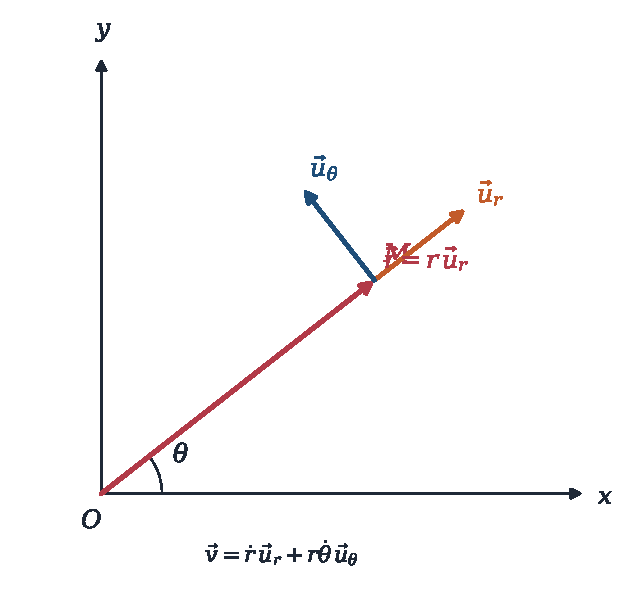
\includegraphics[width=0.66\textwidth]{figures/08_polar_basis.pdf}
\caption{Polar coordinates and the local basis $(\ur,\ut)$. The basis rotates
with the point.}
\label{fig:polar}
\end{figure}

The position vector is simply
\[
\vec r=r\,\ur.
\]
Unlike the Cartesian basis, the polar basis moves:
\[
\frac{\dd\ur}{\dd t}=\dot\theta\,\ut,\qquad
\frac{\dd\ut}{\dd t}=-\dot\theta\,\ur.
\]
Differentiating $\vec r=r\ur$ gives
\[
\vec v=\dot r\,\ur+r\dot\theta\,\ut,
\]
and differentiating again gives
\[
\boxed{\vec a=\left(\ddot r-r\dot\theta^2\right)\ur
+\left(r\ddot\theta+2\dot r\dot\theta\right)\ut.}
\]
The term $-r\dot\theta^2\ur$ is the centripetal acceleration; the term
$2\dot r\dot\theta\,\ut$ is sometimes called the Coriolis term in polar
coordinates.

\begin{keyidea}[Circular motion as a special case]
For a circle, $r=R$ is constant, so $\dot r=\ddot r=0$ and
\[
\vec a=-R\dot\theta^2\,\ur+R\ddot\theta\,\ut
=-\frac{v^2}{R}\ur+a_t\,\ut.
\]
This recovers the centripetal and tangential accelerations of
\cref{ch:plane}.
\end{keyidea}

\section{Cylindrical coordinates}

In three dimensions, cylindrical coordinates $(\rho,\theta,z)$ use the planar
polar coordinates in the $xy$-plane and the Cartesian $z$:
\[
\vec r=\rho\,\vec u_\rho+z\khat.
\]
The velocity and acceleration are
\[
\vec v=\dot\rho\,\vec u_\rho+\rho\dot\theta\,\vec u_\theta+\dot z\,\khat,
\]
\[
\vec a=\left(\ddot\rho-\rho\dot\theta^2\right)\vec u_\rho
+\left(\rho\ddot\theta+2\dot\rho\dot\theta\right)\vec u_\theta
+\ddot z\,\khat.
\]

\section{Spherical coordinates}

Let $r$ be the distance from the origin, $\theta$ the polar angle measured from
the positive $z$-axis, and $\phi$ the azimuthal angle in the $xy$-plane. Then
\[
x=r\sin\theta\cos\phi,\quad
y=r\sin\theta\sin\phi,\quad
z=r\cos\theta.
\]
The position vector is $\vec r=r\,\ur$, and
\[
\vec v=\dot r\,\ur+r\dot\theta\,\ut+r\sin\theta\,\dot\phi\,\uphi.
\]
The acceleration is
\begin{align*}
\vec a={}&\left(\ddot r-r\dot\theta^2-r\sin^2\theta\,\dot\phi^2\right)\ur\\
&+\left(r\ddot\theta+2\dot r\dot\theta-r\sin\theta\cos\theta\,\dot\phi^2\right)\ut\\
&+\left(r\sin\theta\,\ddot\phi+2\dot r\sin\theta\,\dot\phi
+2r\cos\theta\,\dot\theta\dot\phi\right)\uphi.
\end{align*}

\begin{figure}[htbp]
\centering
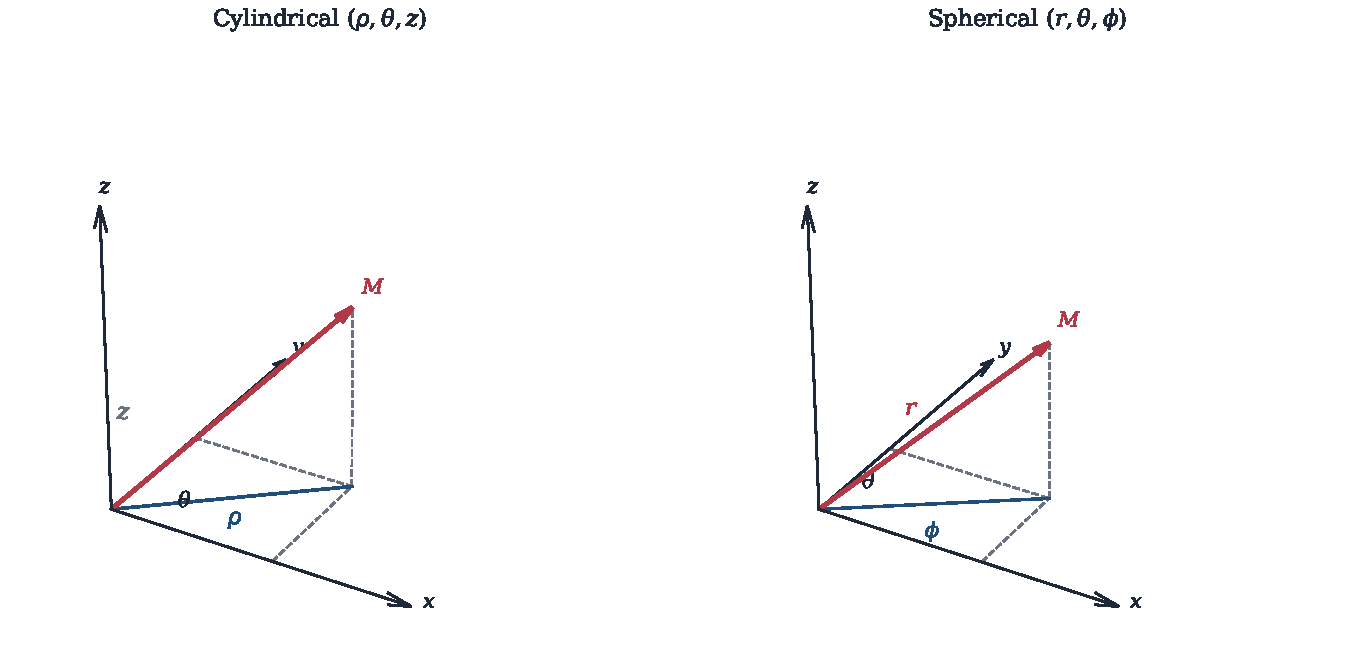
\includegraphics[width=0.98\textwidth]{figures/09_cyl_spherical.pdf}
\caption{Cylindrical coordinates $(\rho,\theta,z)$ and spherical coordinates
$(r,\theta,\phi)$. In the spherical convention used here, $\theta$ is measured
from the $z$-axis.}
\label{fig:cyl-spherical}
\end{figure}

\begin{warning}[Notation varies]
Many books call the azimuthal angle $\theta$ and the polar angle $\phi$. Always
check the definition at the start of a problem. In this book, $\theta$ is the
polar angle from $z$ and $\phi$ is the azimuth in the $xy$-plane.
\end{warning}

\begin{method}[How to use curvilinear coordinates]
\begin{enumerate}[leftmargin=1.5em,itemsep=2pt]
  \item Write down $r(t)$, $\theta(t)$, and (in 3D) $\phi(t)$ or $z(t)$.
  \item Differentiate once to get the general velocity formula.
  \item Differentiate again for acceleration, or use the boxed formulas.
  \item Substitute the time of interest and compute magnitudes with
        $\norm{\vec v}^2=v_r^2+v_\theta^2+v_\phi^2$.
\end{enumerate}
\end{method}

% ===========================================================================
\section{Worked examples}

\begin{worked}[Polar kinematics]
A particle moves in the plane with $r(t)=2t$ (m) and $\theta(t)=t^2$ (rad),
where $t$ is in seconds. Find its velocity and acceleration at
$t=1.00\ \mathrm{s}$.
\end{worked}

\begin{solution}{6.1}
We have
\[
r=2t,\quad \dot r=2,\quad \ddot r=0;\qquad
\theta=t^2,\quad \dot\theta=2t,\quad \ddot\theta=2.
\]
At $t=1$: $r=2$, $\dot r=2$, $\dot\theta=2$, $\ddot\theta=2$, $\ddot r=0$.

Velocity:
\[
\vec v=\dot r\,\ur+r\dot\theta\,\ut
=2\,\ur+2(2)\,\ut=2\,\ur+4\,\ut\ \mathrm{m\,s^{-1}},
\]
\[
v=\sqrt{2^2+4^2}=\sqrt{20}=4.47\ \mathrm{m\,s^{-1}}.
\]
Acceleration:
\[
a_r=\ddot r-r\dot\theta^2=0-2(4)=-8.00\ \mathrm{m\,s^{-2}},
\]
\[
a_\theta=r\ddot\theta+2\dot r\dot\theta=2(2)+2(2)(2)=4+8=12.0\ \mathrm{m\,s^{-2}},
\]
\[
\vec a=-8.00\,\ur+12.0\,\ut\ \mathrm{m\,s^{-2}},\qquad
a=\sqrt{64+144}=14.4\ \mathrm{m\,s^{-2}}.
\]
\end{solution}

\begin{worked}[Motion on a latitude circle]
A particle moves on the sphere of radius $R$ at constant polar angle
$\theta=\pi/3$, with azimuth $\phi=\omega t$. Find its speed and acceleration.
\end{worked}

\begin{solution}{6.2}
Here $r=R$ is constant, $\dot r=\ddot r=0$; $\theta$ is constant, so
$\dot\theta=\ddot\theta=0$; and $\dot\phi=\omega$, $\ddot\phi=0$.

Velocity:
\[
\vec v=r\sin\theta\,\dot\phi\,\uphi
=R\frac{\sqrt3}{2}\omega\,\uphi,
\qquad
v=\frac{\sqrt3}{2}R\omega.
\]
Acceleration:
\[
a_r=-r\sin^2\theta\,\dot\phi^2
=-R\frac34\omega^2,
\]
\[
a_\theta=-r\sin\theta\cos\theta\,\dot\phi^2
=-R\frac{\sqrt3}{2}\frac12\omega^2
=-\frac{\sqrt3}{4}R\omega^2,
\]
\[
a_\phi=0.
\]
Thus
\[
\vec a=-\frac34R\omega^2\,\ur-\frac{\sqrt3}{4}R\omega^2\,\ut,
\qquad
a=\sqrt{\frac{9}{16}+\frac{3}{16}}\,R\omega^2
=\frac{\sqrt3}{2}R\omega^2.
\]
Note that $a=v^2/\rho$, where $\rho=R\sin\theta$ is the radius of the latitude
circle.
\end{solution}

% ===========================================================================
\section{Exercises and Step-by-Step Solutions}

\begin{exercise}{\warm\ Coordinate conversion}
Convert the Cartesian point $(2,-2,3)$ to cylindrical and spherical coordinates.
\end{exercise}

\begin{tabletworkspace}[6.5cm]
\end{tabletworkspace}

\begin{solution}{6.1}
Cylindrical:
\[
\rho=\sqrt{x^2+y^2}=\sqrt{4+4}=\sqrt8=2.83,
\]
\[
\theta=\arctan\frac{y}{x}=\arctan(-1)=-45.0^\circ
\]
(the point is in the fourth quadrant), and $z=3.00$.

Spherical:
\[
r=\sqrt{x^2+y^2+z^2}=\sqrt{4+4+9}=\sqrt{17}=4.12,
\]
\[
\theta=\arccos\frac{z}{r}=\arccos\frac{3}{4.12}=43.3^\circ,
\]
and $\phi=-45.0^\circ$.
\end{solution}

\begin{exercise}{\warm\ Uniform circular motion in polar form}
A particle moves on a circle of radius $3.00\ \mathrm{m}$ with
$\theta(t)=2.00t$ rad. Find its velocity and acceleration at
$t=1.00\ \mathrm{s}$ using polar coordinates.
\end{exercise}

\begin{tabletworkspace}[6.5cm]
\end{tabletworkspace}

\begin{solution}{6.2}
With $r=R=3.00$ constant, $\dot r=\ddot r=0$, and
$\dot\theta=2.00$, $\ddot\theta=0$:
\[
\vec v=R\dot\theta\,\ut=3.00(2.00)\,\ut=6.00\,\ut\ \mathrm{m\,s^{-1}},
\]
\[
v=6.00\ \mathrm{m\,s^{-1}}.
\]
\[
a_r=-R\dot\theta^2=-3.00(4.00)=-12.0\ \mathrm{m\,s^{-2}},
\]
\[
a_\theta=R\ddot\theta=0.
\]
Thus
\[
\vec a=-12.0\,\ur\ \mathrm{m\,s^{-2}},
\qquad a=12.0\ \mathrm{m\,s^{-2}}
\]
toward the centre.
\end{solution}

\begin{exercise}{\warm\ Polar kinematics}
A particle has $r(t)=t^2$ (m) and $\theta(t)=t$ (rad). Find $\vec v$ and
$\vec a$ at $t=2.00\ \mathrm{s}$, and their magnitudes.
\end{exercise}

\begin{tabletworkspace}[6.5cm]
\end{tabletworkspace}

\begin{solution}{6.3}
\[
r=t^2\implies \dot r=2t,\ \ddot r=2;\qquad
\theta=t\implies \dot\theta=1,\ \ddot\theta=0.
\]
At $t=2$: $r=4$, $\dot r=4$, $\dot\theta=1$.

\[
\vec v=4\,\ur+4(1)\,\ut=4\,\ur+4\,\ut\ \mathrm{m\,s^{-1}},
\qquad v=4\sqrt2=5.66\ \mathrm{m\,s^{-1}}.
\]
\[
a_r=\ddot r-r\dot\theta^2=2-4(1)=-2.00\ \mathrm{m\,s^{-2}},
\]
\[
a_\theta=r\ddot\theta+2\dot r\dot\theta=0+2(4)(1)=8.00\ \mathrm{m\,s^{-2}}.
\]
\[
\vec a=-2.00\,\ur+8.00\,\ut\ \mathrm{m\,s^{-2}},
\qquad a=\sqrt{4+64}=8.25\ \mathrm{m\,s^{-2}}.
\]
\end{solution}

\begin{exercise}{\core\ Radial oscillation}
A particle moves with $r(t)=2+\cos t$ (m) and $\theta(t)=t$ (rad). Find
$\vec v$ and $\vec a$ at $t=\pi/2$.
\end{exercise}

\begin{tabletworkspace}[6.5cm]
\end{tabletworkspace}

\begin{solution}{6.4}
\[
r=2+\cos t\implies \dot r=-\sin t,\ \ddot r=-\cos t.
\]
At $t=\pi/2$: $r=2$, $\dot r=-1$, $\ddot r=0$; and $\theta=t$ gives
$\dot\theta=1$, $\ddot\theta=0$.

\[
\vec v=\dot r\,\ur+r\dot\theta\,\ut=-\ur+2\ut\ \mathrm{m\,s^{-1}},
\qquad v=\sqrt{1+4}=\sqrt5=2.24\ \mathrm{m\,s^{-1}}.
\]
\[
a_r=\ddot r-r\dot\theta^2=0-2(1)=-2.00\ \mathrm{m\,s^{-2}},
\]
\[
a_\theta=r\ddot\theta+2\dot r\dot\theta=0+2(-1)(1)=-2.00\ \mathrm{m\,s^{-2}}.
\]
\[
\vec a=-2.00\,\ur-2.00\,\ut\ \mathrm{m\,s^{-2}},
\qquad a=\sqrt{8}=2.83\ \mathrm{m\,s^{-2}}.
\]
\end{solution}

\begin{exercise}{\core\ Cylindrical motion}
A particle has $\rho=2.00\ \mathrm{m}$ (constant), $\theta=3.00t$ rad, and
$z=4.00t^2$ m. Find its velocity and acceleration at $t=1.00\ \mathrm{s}$.
\end{exercise}

\begin{tabletworkspace}[6.5cm]
\end{tabletworkspace}

\begin{solution}{6.5}
\[
\rho=2,\ \dot\rho=0,\ \ddot\rho=0;\qquad
\theta=3t,\ \dot\theta=3,\ \ddot\theta=0;\qquad
z=4t^2,\ \dot z=8t,\ \ddot z=8.
\]
At $t=1$: $\dot z=8.00$, $\ddot z=8.00$.

\[
\vec v=\rho\dot\theta\,\vec u_\theta+\dot z\,\khat
=2(3)\vec u_\theta+8\khat=6.00\,\vec u_\theta+8.00\,\khat\ \mathrm{m\,s^{-1}},
\]
\[
v=\sqrt{36+64}=10.0\ \mathrm{m\,s^{-1}}.
\]
\[
a_\rho=-\rho\dot\theta^2=-2(9)=-18.0\ \mathrm{m\,s^{-2}},
\]
\[
a_\theta=\rho\ddot\theta+2\dot\rho\dot\theta=0,
\]
\[
a_z=\ddot z=8.00\ \mathrm{m\,s^{-2}}.
\]
\[
\vec a=-18.0\,\vec u_\rho+8.00\,\khat\ \mathrm{m\,s^{-2}},
\qquad a=\sqrt{324+64}=19.7\ \mathrm{m\,s^{-2}}.
\]
\end{solution}

\begin{exercise}{\core\ Motion on the equator}
A particle moves on the equator of a sphere of radius $R$ with azimuth
$\phi=\omega t$. Use spherical coordinates to find its speed and acceleration.
\end{exercise}

\begin{tabletworkspace}[6.5cm]
\end{tabletworkspace}

\begin{solution}{6.6}
On the equator, $\theta=\pi/2$ is constant, so
$\dot\theta=\ddot\theta=0$, and $r=R$ is constant. With $\dot\phi=\omega$,
\[
\vec v=R\sin\frac{\pi}{2}\,\omega\,\uphi=R\omega\,\uphi,
\qquad v=R\omega.
\]
The acceleration components are
\[
a_r=-R\sin^2\frac{\pi}{2}\,\omega^2=-R\omega^2,
\]
\[
a_\theta=-R\sin\frac{\pi}{2}\cos\frac{\pi}{2}\,\omega^2=0,
\qquad a_\phi=0.
\]
Thus
\[
\vec a=-R\omega^2\,\ur,
\]
which is the familiar centripetal acceleration toward the centre of the sphere.
\end{solution}

\begin{exercise}{\core\ Derivatives of the polar basis}
Starting from
$\ur=\cos\theta\,\ihat+\sin\theta\,\jhat$ and
$\ut=-\sin\theta\,\ihat+\cos\theta\,\jhat$, prove that
\[
\frac{\dd\ur}{\dd t}=\dot\theta\,\ut,\qquad
\frac{\dd\ut}{\dd t}=-\dot\theta\,\ur.
\]
\end{exercise}

\begin{tabletworkspace}[6.5cm]
\end{tabletworkspace}

\begin{solution}{6.7}
Differentiate $\ur$:
\[
\frac{\dd\ur}{\dd t}
=-\sin\theta\,\dot\theta\,\ihat+\cos\theta\,\dot\theta\,\jhat
=\dot\theta(-\sin\theta\,\ihat+\cos\theta\,\jhat)
=\dot\theta\,\ut.
\]
Similarly,
\[
\frac{\dd\ut}{\dd t}
=-\cos\theta\,\dot\theta\,\ihat-\sin\theta\,\dot\theta\,\jhat
=-\dot\theta(\cos\theta\,\ihat+\sin\theta\,\jhat)
=-\dot\theta\,\ur.
\]
\end{solution}

\begin{exercise}{\core\ Circular motion from the general formula}
Starting from the general polar acceleration, set $r=R=$ constant and recover
\[
\vec a=-\frac{v^2}{R}\ur+a_t\,\ut.
\]
Identify $v$ and $a_t$ in terms of $\theta$.
\end{exercise}

\begin{tabletworkspace}[6.5cm]
\end{tabletworkspace}

\begin{solution}{6.8}
For $r=R$, $\dot r=\ddot r=0$. The general formulas give
\[
\vec a=-R\dot\theta^2\,\ur+R\ddot\theta\,\ut.
\]
The speed is $v=R\dot\theta$, so
\[
R\dot\theta^2=\frac{(R\dot\theta)^2}{R}=\frac{v^2}{R}.
\]
The tangential acceleration is
\[
a_t=\frac{\dd v}{\dd t}=R\ddot\theta.
\]
Hence
\[
\vec a=-\frac{v^2}{R}\ur+R\ddot\theta\,\ut
=-\frac{v^2}{R}\ur+a_t\,\ut.
\]
\end{solution}

\begin{exercise}{\mastery\ Conservation of areal velocity}
For a central force the transverse acceleration vanishes: $a_\theta=0$. Show
that this implies
\[
r^2\dot\theta=\text{constant}.
\]
Interpret this constant geometrically as twice the areal velocity.
\end{exercise}

\begin{tabletworkspace}[6.5cm]
\end{tabletworkspace}

\begin{solution}{6.9}
The transverse acceleration is
\[
a_\theta=r\ddot\theta+2\dot r\dot\theta
=\frac1r\frac{\dd}{\dd t}\left(r^2\dot\theta\right).
\]
If $a_\theta=0$, then
\[
\frac{\dd}{\dd t}\left(r^2\dot\theta\right)=0
\implies
r^2\dot\theta=h=\text{constant}.
\]
In polar coordinates the area swept by the radius vector in time $\dd t$ is
\[
\dd A=\frac12r^2\,\dd\theta,
\]
so the areal velocity is
\[
\frac{\dd A}{\dd t}=\frac12r^2\dot\theta=\frac h2,
\]
which is constant. This is Kepler's second law.
\end{solution}

\begin{exercise}{\mastery\ Logarithmic spiral}
A particle moves with $r(t)=ae^{bt}$ and $\theta(t)=ct$, where $a,b,c$ are
constants. Find the radial and transverse components of velocity and
acceleration. Show that the acceleration makes a constant angle with the radial
direction.
\end{exercise}

\begin{tabletworkspace}[6.5cm]
\end{tabletworkspace}

\begin{solution}{6.10}
With $r=ae^{bt}$,
\[
\dot r=ab\,e^{bt},\qquad \ddot r=ab^2e^{bt},
\]
and with $\theta=ct$, $\dot\theta=c$, $\ddot\theta=0$. Therefore
\[
v_r=\dot r=ab\,e^{bt},\qquad
v_\theta=r\dot\theta=ac\,e^{bt},
\]
so
\[
\vec v=ae^{bt}\left(b\,\ur+c\,\ut\right).
\]
For the acceleration,
\[
a_r=\ddot r-r\dot\theta^2
=ae^{bt}\left(b^2-c^2\right),
\]
\[
a_\theta=r\ddot\theta+2\dot r\dot\theta
=2abc\,e^{bt}.
\]
Thus
\[
\vec a=ae^{bt}\left[(b^2-c^2)\,\ur+2bc\,\ut\right].
\]
The ratio $a_\theta/a_r=2bc/(b^2-c^2)$ is independent of time, so the acceleration
makes a constant angle with the radial direction. The curve is a logarithmic
spiral.
\end{solution}


\chapter{Relative and Composite Motion}
\label{ch:relative}
\begin{chapterintro}
\textbf{You will learn to:} transform velocities and accelerations between
reference frames; use the composition laws; analyse motion in a rotating frame;
and identify the Coriolis and centrifugal terms.
\end{chapterintro}

\section{Galilean transformation}

Let $R(O,x,y,z)$ be a fixed frame and $R'(O',x',y',z')$ a frame moving with
constant velocity $\vec V$ relative to $R$, without rotation. Then
\[
\vec r=\vec r'+\vec Vt,\qquad
\vec v=\vec v'+\vec V,\qquad
\vec a=\vec a'.
\]
The acceleration is the same in both frames. Such frames are \textbf{inertial}:
Newton's laws have the same form in all of them. This is Galilean relativity.

\section{Composition of velocities and accelerations}

For a general moving frame (translating and rotating), let
\begin{itemize}[leftmargin=1.4em,itemsep=2pt]
  \item $\vec v_a$ be the absolute velocity (relative to $R$);
  \item $\vec v_r$ the relative velocity (relative to $R'$);
  \item $\vec v_e$ the entrainment (drag) velocity, i.e.\ the velocity in $R$ of
        the point of $R'$ coinciding with $M$.
\end{itemize}
Then
\[
\boxed{\vec v_a=\vec v_r+\vec v_e.}
\]
For a frame rotating with angular velocity $\vec\Omega$,
\[
\vec v_e=\vec v(O'/R)+\vec\Omega\times\vec{O'M}.
\]
The acceleration composition law is
\[
\boxed{\vec a_a=\vec a_r+\vec a_e+\vec a_c,}
\]
where
\[
\vec a_e=\vec a(O'/R)+\frac{\dd\vec\Omega}{\dd t}\times\vec{O'M}
+\vec\Omega\times\left(\vec\Omega\times\vec{O'M}\right),
\]
and the \textbf{Coriolis acceleration} is
\[
\vec a_c=2\vec\Omega\times\vec v_r.
\]

\begin{figure}[htbp]
\centering
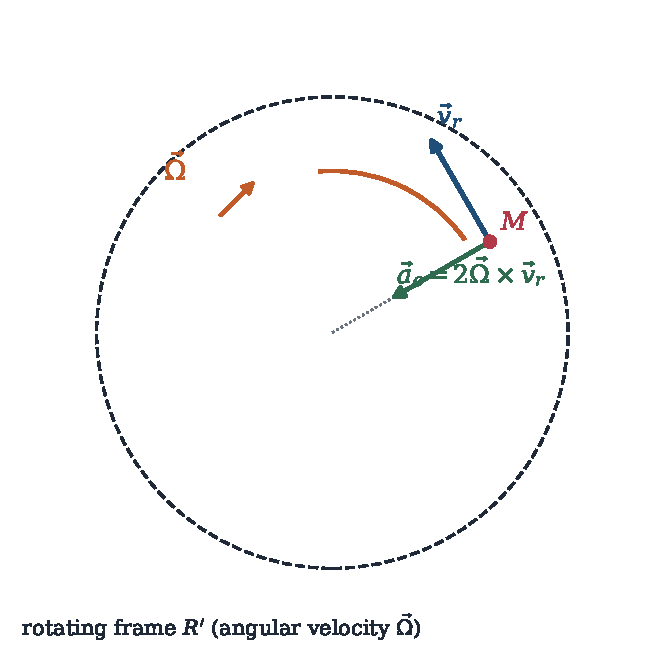
\includegraphics[width=0.72\textwidth]{figures/10_rotating_frame.pdf}
\caption{A point $M$ moving in a rotating frame. The Coriolis acceleration is
perpendicular to both the angular velocity and the relative velocity.}
\label{fig:rotating-frame}
\end{figure}

\section{Non-inertial frames and fictitious forces}

Newton's second law in an inertial frame is $m\vec a_a=\vec F$. Using the
composition law,
\[
m\vec a_r=\vec F-m\vec a_e-m\vec a_c.
\]
The last two terms behave like additional forces in the rotating frame:
\[
\vec F_{\text{Coriolis}}=-2m\vec\Omega\times\vec v_r,\qquad
\vec F_{\text{centrifugal}}=-m\vec\Omega\times(\vec\Omega\times\vec r').
\]
They are called \textbf{fictitious} or \textbf{inertial} forces because they
disappear in an inertial frame.

\begin{keyidea}[Boat problems]
In a river, the entrainment velocity is the current. The boat's velocity relative
to the water is $\vec v_r$; the velocity relative to the bank is
$\vec v_a=\vec v_r+\vec v_e$. Draw the vector triangle before computing.
\end{keyidea}

% ===========================================================================
\section{Worked examples}

\begin{worked}[Crossing a river]
A boat has speed $5.00\ \mathrm{m\,s^{-1}}$ relative to the water. A river of
width $100\ \mathrm{m}$ flows at $3.00\ \mathrm{m\,s^{-1}}$.
(a) If the boat heads straight across, find the crossing time and the downstream
drift.
(b) At what angle upstream must it head to land directly opposite? Find the
crossing time.
\end{worked}

\begin{solution}{7.1}
(a) Heading straight across, the cross-stream component is
$v_{r,\perp}=5.00\ \mathrm{m\,s^{-1}}$, so
\[
t=\frac{d}{v_{r,\perp}}=\frac{100}{5.00}=20.0\ \mathrm{s}.
\]
The downstream drift is
\[
x=v_e t=3.00(20.0)=60.0\ \mathrm{m}.
\]
The speed relative to the bank is
$\sqrt{5.00^2+3.00^2}=5.83\ \mathrm{m\,s^{-1}}$.

(b) To cancel the current, the upstream component must satisfy
\[
v_r\sin\theta=v_e
\implies
5.00\sin\theta=3.00
\implies
\theta=36.9^\circ
\]
upstream from the perpendicular direction. The cross-stream component is
\[
v_r\cos\theta=5.00\cos36.9^\circ=4.00\ \mathrm{m\,s^{-1}},
\]
so
\[
t=\frac{100}{4.00}=25.0\ \mathrm{s}.
\]
\end{solution}

\begin{worked}[Motion on a rotating disk]
A disk rotates with constant angular velocity
$\Omega=2.00\ \mathrm{rad\,s^{-1}}$. A bead moves radially outward along a
groove at constant relative speed $v_r=0.500\ \mathrm{m\,s^{-1}}$. At the instant
when $r=1.00\ \mathrm{m}$, find the absolute velocity and acceleration of the
bead.
\end{worked}

\begin{solution}{7.2}
Take $\vec\Omega=\Omega\khat$ and $\vec v_r=v_r\vec u_r$. The entrainment
velocity is
\[
v_e=\Omega r=2.00(1.00)=2.00\ \mathrm{m\,s^{-1}}
\]
in the tangential direction. Thus
\[
\vec v_a=0.500\,\vec u_r+2.00\,\vec u_\theta,
\qquad
v_a=\sqrt{0.25+4.00}=2.06\ \mathrm{m\,s^{-1}}.
\]
The relative acceleration is zero (constant radial speed). The entrainment
acceleration is
\[
\vec a_e=\vec\Omega\times(\vec\Omega\times\vec r)
=-\Omega^2r\,\vec u_r=-4.00\,\vec u_r\ \mathrm{m\,s^{-2}}.
\]
The Coriolis acceleration is
\[
\vec a_c=2\vec\Omega\times\vec v_r
=2(2.00)(0.500)\,\vec u_\theta=2.00\,\vec u_\theta\ \mathrm{m\,s^{-2}}.
\]
Therefore
\[
\vec a_a=-4.00\,\vec u_r+2.00\,\vec u_\theta\ \mathrm{m\,s^{-2}},
\qquad
a_a=\sqrt{16+4}=4.47\ \mathrm{m\,s^{-2}}.
\]
\end{solution}

% ===========================================================================
\section{Exercises and Step-by-Step Solutions}

\begin{exercise}{\warm\ Walking on a train}
A train moves at $20.0\ \mathrm{m\,s^{-1}}$ relative to the ground. A passenger
walks at $2.00\ \mathrm{m\,s^{-1}}$ relative to the train. Find the passenger's
velocity relative to the ground when walking (a) forward and (b) backward.
\end{exercise}

\begin{tabletworkspace}[6.5cm]
\end{tabletworkspace}

\begin{solution}{7.1}
(a) Forward:
\[
v=20.0+2.00=22.0\ \mathrm{m\,s^{-1}}.
\]
(b) Backward:
\[
v=20.0-2.00=18.0\ \mathrm{m\,s^{-1}}.
\]
\end{solution}

\begin{exercise}{\warm\ Rain and walking}
Rain falls vertically at $8.00\ \mathrm{m\,s^{-1}}$. A person walks horizontally
at $6.00\ \mathrm{m\,s^{-1}}$. Find the magnitude and direction of the rain's
velocity relative to the person.
\end{exercise}

\begin{tabletworkspace}[6.5cm]
\end{tabletworkspace}

\begin{solution}{7.2}
The velocity of the rain relative to the person is
\[
\vec v_{rp}=\vec v_{\text{rain}}-\vec v_{\text{person}}.
\]
With the rain vertical and the person horizontal,
\[
v_{rp}=\sqrt{8.00^2+6.00^2}=10.0\ \mathrm{m\,s^{-1}}.
\]
The angle from the vertical satisfies
\[
\tan\theta=\frac{6.00}{8.00}=0.750
\implies
\theta=36.9^\circ.
\]
The rain appears to come from ahead, at $36.9^\circ$ from the vertical.
\end{solution}

\begin{exercise}{\warm\ Straight across a river}
A boat has speed $4.00\ \mathrm{m\,s^{-1}}$ relative to the water. The river is
$200\ \mathrm{m}$ wide and flows at $2.00\ \mathrm{m\,s^{-1}}$. If the boat heads
straight across, find the crossing time, the downstream drift, and the speed
relative to the bank.
\end{exercise}

\begin{tabletworkspace}[6.5cm]
\end{tabletworkspace}

\begin{solution}{7.3}
Heading straight across, the cross-stream speed is $4.00\ \mathrm{m\,s^{-1}}$:
\[
t=\frac{200}{4.00}=50.0\ \mathrm{s}.
\]
The drift is
\[
x=v_e t=2.00(50.0)=100\ \mathrm{m}.
\]
The speed relative to the bank is
\[
v=\sqrt{4.00^2+2.00^2}=\sqrt{20.0}=4.47\ \mathrm{m\,s^{-1}}.
\]
\end{solution}

\begin{exercise}{\core\ Landing directly opposite}
Repeat the river of the previous exercise, but now find the heading angle
required to land directly opposite the starting point, and the corresponding
crossing time.
\end{exercise}

\begin{tabletworkspace}[6.5cm]
\end{tabletworkspace}

\begin{solution}{7.4}
To land directly opposite, the upstream component of the boat's velocity must
cancel the current:
\[
4.00\sin\theta=2.00
\implies
\sin\theta=0.500
\implies
\theta=30.0^\circ.
\]
The cross-stream component is
\[
4.00\cos30.0^\circ=3.46\ \mathrm{m\,s^{-1}},
\]
so
\[
t=\frac{200}{3.46}=57.7\ \mathrm{s}.
\]
\end{solution}

\begin{exercise}{\core\ Relative velocity of two cars}
Car A travels east at $25.0\ \mathrm{m\,s^{-1}}$; car B travels north at
$15.0\ \mathrm{m\,s^{-1}}$. Find the velocity of B relative to A: magnitude and
direction.
\end{exercise}

\begin{tabletworkspace}[6.5cm]
\end{tabletworkspace}

\begin{solution}{7.5}
Take east as $+x$ and north as $+y$:
\[
\vec v_A=(25.0,0),\qquad \vec v_B=(0,15.0).
\]
\[
\vec v_{B/A}=\vec v_B-\vec v_A=(-25.0,\,15.0)\ \mathrm{m\,s^{-1}}.
\]
\[
\norm{\vec v_{B/A}}=\sqrt{625+225}=\sqrt{850}=29.2\ \mathrm{m\,s^{-1}}.
\]
The direction is
\[
\theta=\arctan\frac{15.0}{-25.0}.
\]
The vector points northwest; measured from east,
$\theta=180^\circ-31.0^\circ=149^\circ$.
\end{solution}

\begin{exercise}{\core\ Bead on a rotating disk}
A disk rotates at $\Omega=3.00\ \mathrm{rad\,s^{-1}}$. A bead moves radially
outward at constant relative speed $v_r=2.00\ \mathrm{m\,s^{-1}}$. At
$r=0.500\ \mathrm{m}$, find the absolute velocity and the Coriolis and
centrifugal accelerations.
\end{exercise}

\begin{tabletworkspace}[6.5cm]
\end{tabletworkspace}

\begin{solution}{7.6}
The entrainment velocity is
\[
v_e=\Omega r=3.00(0.500)=1.50\ \mathrm{m\,s^{-1}}
\]
tangential. Thus
\[
\vec v_a=2.00\,\vec u_r+1.50\,\vec u_\theta,
\qquad
v_a=\sqrt{4.00+2.25}=2.50\ \mathrm{m\,s^{-1}}.
\]
The Coriolis acceleration has magnitude
\[
a_c=2\Omega v_r=2(3.00)(2.00)=12.0\ \mathrm{m\,s^{-2}}
\]
in the tangential direction. The centrifugal acceleration has magnitude
\[
\Omega^2r=(3.00)^2(0.500)=4.50\ \mathrm{m\,s^{-2}}
\]
directed outward. (The entrainment acceleration
$\vec\Omega\times(\vec\Omega\times\vec r)$ points inward with this magnitude.)
\end{solution}

\begin{exercise}{\core\ Coriolis on Earth}
At latitude $45.0^\circ$, an object moves horizontally eastward at
$100\ \mathrm{m\,s^{-1}}$. Taking the Earth's angular velocity as
$\Omega=7.29\times10^{-5}\ \mathrm{rad\,s^{-1}}$, estimate the magnitude of the
horizontal Coriolis acceleration.
\end{exercise}

\begin{tabletworkspace}[6.5cm]
\end{tabletworkspace}

\begin{solution}{7.7}
The horizontal Coriolis acceleration at latitude $\lambda$ for a horizontal
velocity has magnitude
\[
a_C=2\Omega v\sin\lambda.
\]
Thus
\[
a_C=2(7.29\times10^{-5})(100)\sin45.0^\circ
=1.03\times10^{-2}\ \mathrm{m\,s^{-2}}.
\]
This is small but not negligible over long times; it is what causes the
deflection of long-range projectiles and cyclones.
\end{solution}

\begin{exercise}{\core\ Galilean invariance}
Show that Newton's second law $m\vec a=\vec F$ is unchanged under the Galilean
transformation $\vec r=\vec r'+\vec Vt$ with constant $\vec V$.
\end{exercise}

\begin{tabletworkspace}[6.5cm]
\end{tabletworkspace}

\begin{solution}{7.8}
Under $\vec r=\vec r'+\vec Vt$ with $\vec V$ constant,
\[
\vec v=\vec v'+\vec V,\qquad
\vec a=\frac{\dd\vec v'}{\dd t}+\frac{\dd\vec V}{\dd t}=\vec a'.
\]
Therefore
\[
m\vec a'=m\vec a=\vec F.
\]
The equation of motion has the same form in both frames, so the frames are
inertial.
\end{solution}

\begin{exercise}{\mastery\ Deriving the composition law}
A frame $R'$ rotates with angular velocity $\vec\Omega(t)$ relative to $R$.
Starting from $\vec r=\vec r'$ (common origin), derive
\[
\vec v_a=\vec v_r+\vec\Omega\times\vec r',
\]
and then
\[
\vec a_a=\vec a_r+2\vec\Omega\times\vec v_r
+\vec\Omega\times(\vec\Omega\times\vec r')
+\frac{\dd\vec\Omega}{\dd t}\times\vec r'.
\]
\end{exercise}

\begin{tabletworkspace}[6.5cm]
\end{tabletworkspace}

\begin{solution}{7.9}
Let $\vec r'$ have constant components in $R'$. The time derivative in $R$ is
\[
\left(\frac{\dd\vec r'}{\dd t}\right)_R
=\left(\frac{\dd\vec r'}{\dd t}\right)_{R'}
+\vec\Omega\times\vec r'
=\vec v_r+\vec\Omega\times\vec r',
\]
which gives the velocity law. Applying the same operator to
$\vec v_a=\vec v_r+\vec\Omega\times\vec r'$:
\[
\vec a_a=\left(\frac{\dd\vec v_r}{\dd t}\right)_R
+\frac{\dd\vec\Omega}{\dd t}\times\vec r'
+\vec\Omega\times\left(\frac{\dd\vec r'}{\dd t}\right)_R.
\]
Now
\[
\left(\frac{\dd\vec v_r}{\dd t}\right)_R=\vec a_r+\vec\Omega\times\vec v_r,
\]
and
\[
\left(\frac{\dd\vec r'}{\dd t}\right)_R=\vec v_r+\vec\Omega\times\vec r'.
\]
Substituting,
\[
\vec a_a=\vec a_r+\vec\Omega\times\vec v_r
+\frac{\dd\vec\Omega}{\dd t}\times\vec r'
+\vec\Omega\times\vec v_r
+\vec\Omega\times(\vec\Omega\times\vec r').
\]
The two $\vec\Omega\times\vec v_r$ terms combine to $2\vec\Omega\times\vec v_r$,
giving the stated result.
\end{solution}

\begin{exercise}{\mastery\ Ball thrown in an accelerating train}
A train accelerates at $2.00\ \mathrm{m\,s^{-2}}\). A passenger throws a ball
vertically upward with speed $5.00\ \mathrm{m\,s^{-1}}$ relative to the train.
(a) Find the time of flight.
(b) Find where the ball lands relative to the thrower in the train.
(c) Explain the result using the composition law.
\end{exercise}

\begin{tabletworkspace}[6.5cm]
\end{tabletworkspace}

\begin{solution}{7.10}
(a) In the train frame, the ball moves vertically with acceleration $-g$. Its
time of flight is
\[
t=\frac{2v_0}{g}=\frac{2(5.00)}{9.81}=1.02\ \mathrm{s}.
\]
(b) During this time the train moves forward a distance
\[
s=\frac12at^2=\frac12(2.00)(1.02)^2=1.04\ \mathrm{m}.
\]
In the train frame the ball lands $1.04\ \mathrm{m}$ behind the thrower.
(c) In the ground frame the ball keeps the horizontal velocity it had at launch
(the train's velocity at that instant) because no horizontal force acts on it.
The train, however, continues to accelerate. The train therefore moves ahead of
the ball, so in the train frame the ball appears to be deflected backward. This
is the effect of the fictitious force $-m\vec a_{\text{train}}$ in the
non-inertial frame.
\end{solution}



\part{Dynamics}

\chapter{Newton's Laws and Free-Body Diagrams}
\label{ch:newton}
\begin{chapterintro}
\textbf{You will learn to:} state Newton's three laws; draw a correct free-body
diagram; write the equations of motion along convenient axes; and solve
equilibrium and circular-motion problems.
\end{chapterintro}

\section{Newton's laws}

\begin{enumerate}[leftmargin=1.7em,itemsep=4pt]
  \item \textbf{Inertia.} In an inertial frame, a body remains at rest or in
        uniform rectilinear motion unless acted on by a net external force.
  \item \textbf{Fundamental principle of dynamics.}
        \[
        \sum\vec F_{\text{ext}}
        =\frac{\dd\vec p}{\dd t}
        =\frac{\dd(m\vec v)}{\dd t}.
        \]
        For constant mass,
        \[
        \boxed{\sum\vec F_{\text{ext}}=m\vec a.}
        \]
  \item \textbf{Action--reaction.} If $A$ exerts a force on $B$, then $B$ exerts
        on $A$ a force equal in magnitude and opposite in direction:
        \[
        \vec F_{B\to A}=-\vec F_{A\to B}.
        \]
\end{enumerate}

The three laws are valid in an \textbf{inertial frame}. A frame accelerating or
rotating relative to an inertial frame requires the fictitious forces of
\cref{ch:relative}.

\section{Standard force models}

\begin{center}
\renewcommand{\arraystretch}{1.3}
\begin{tabular}{@{}p{0.22\textwidth}p{0.34\textwidth}p{0.36\textwidth}@{}}
\toprule
\textbf{Force} & \textbf{Expression} & \textbf{Direction} \\
\midrule
Weight & $\vec W=m\vec g$ & vertical, downward \\
Normal reaction & $\vec N$ & perpendicular to the surface, away from it \\
Tension & $T$ & along the string, pulling the body \\
Spring (Hooke) & $\vec F=-k(l-l_0)\vec u$ & toward the equilibrium position \\
Solid friction & $f\le\mu_sN$, $f_k=\mu_kN$ & opposite to the tendency of sliding \\
Viscous drag & $\vec f=-k\vec v$ & opposite to the velocity \\
Universal gravity & $\vec F=-GMm\,\ur/r^2$ & attractive, toward the other mass \\
\bottomrule
\end{tabular}
\end{center}

\begin{figure}[htbp]
\centering
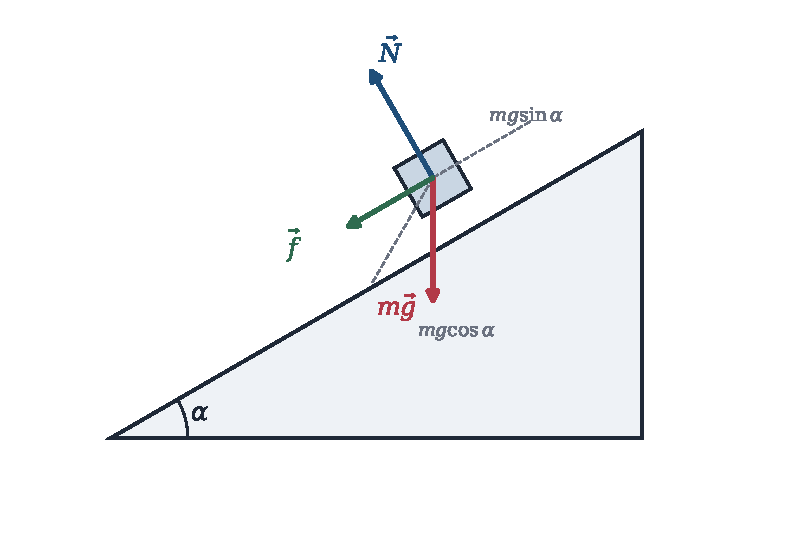
\includegraphics[width=0.82\textwidth]{figures/11_incline_fbd.pdf}
\caption{Free-body diagram for a block on an inclined plane. The weight is
decomposed into components parallel and perpendicular to the plane.}
\label{fig:incline-fbd}
\end{figure}

\section{The free-body diagram method}

\begin{method}[Five steps that solve most problems]
\begin{enumerate}[leftmargin=1.6em,itemsep=2pt]
  \item Isolate the body of interest.
  \item Draw every external force acting \emph{on} it (not forces it exerts on
        other bodies).
  \item Choose axes: along the motion and perpendicular to it.
  \item Decompose the forces along the axes.
  \item Apply $\sum F_x=ma_x$, $\sum F_y=ma_y$. If the body does not accelerate
        in a direction, the sum of forces in that direction is zero.
\end{enumerate}
\end{method}

\begin{warning}[Two classic errors]
Do not put both the weight $m\vec g$ and its components $mg\sin\alpha$,
$mg\cos\alpha$ on the same diagram: choose one representation. Do not include
the force that the body exerts on something else; the diagram is only about
forces \emph{on} the body.
\end{warning}

\section{Dynamics of circular motion}

For a particle moving on a circle of radius $R$, project Newton's second law on
the inward radial direction and on the tangent:
\[
\sum F_{\text{radial}}=m\frac{v^2}{R},
\qquad
\sum F_{\text{tangential}}=m\frac{\dd v}{\dd t}.
\]
The radial equation is not a new law; it is $m\vec a$ written in the normal and
tangential directions.

% ===========================================================================
\section{Worked examples}

\begin{worked}[Block on a frictionless incline]
A block of mass $m=5.00\ \mathrm{kg}$ rests on a frictionless plane inclined at
$\alpha=30.0^\circ$. Find its acceleration and the normal reaction.
\end{worked}

\begin{solution}{8.1}
Take axes parallel and perpendicular to the plane. The only forces are the weight
$m\vec g$ and the normal $\vec N$. The weight components are
$mg\sin\alpha$ down the slope and $mg\cos\alpha$ into the plane.

Perpendicular to the plane there is no acceleration:
\[
N-mg\cos\alpha=0
\implies
N=mg\cos\alpha.
\]
Parallel to the plane:
\[
mg\sin\alpha=ma
\implies
a=g\sin\alpha.
\]
Numerically,
\[
a=9.81\sin30.0^\circ=4.91\ \mathrm{m\,s^{-2}},
\]
\[
N=5.00(9.81)\cos30.0^\circ=42.5\ \mathrm{N}.
\]
\end{solution}

\begin{worked}[Apparent weight in an elevator]
A person of mass $m=70.0\ \mathrm{kg}$ stands on a scale in an elevator. Find the
scale reading when the elevator (a) is at rest, (b) accelerates upward at
$2.00\ \mathrm{m\,s^{-2}}$, (c) accelerates downward at $2.00\ \mathrm{m\,s^{-2}}$,
and (d) is in free fall.
\end{worked}

\begin{solution}{8.2}
The scale reads the normal force $N$. Take upward as positive. Newton's second
law:
\[
N-mg=ma
\implies
N=m(g+a).
\]
(a) $a=0$:
\[
N=70.0(9.81)=687\ \mathrm{N}.
\]
(b) $a=+2.00\ \mathrm{m\,s^{-2}}$:
\[
N=70.0(9.81+2.00)=827\ \mathrm{N}.
\]
(c) $a=-2.00\ \mathrm{m\,s^{-2}}$:
\[
N=70.0(9.81-2.00)=547\ \mathrm{N}.
\]
(d) $a=-g$:
\[
N=70.0(9.81-9.81)=0.
\]
The person feels weightless.
\end{solution}

% ===========================================================================
\section{Exercises and Step-by-Step Solutions}

\begin{exercise}{\warm\ Newton's second law}
A net force of $30.0\ \mathrm{N}$ acts on a $10.0\ \mathrm{kg}$ body initially at
rest. Find its acceleration, its speed after $4.00\ \mathrm{s}$, and the distance
travelled.
\end{exercise}

\begin{tabletworkspace}[6.5cm]
\end{tabletworkspace}

\begin{solution}{8.1}
\[
a=\frac Fm=\frac{30.0}{10.0}=3.00\ \mathrm{m\,s^{-2}}.
\]
\[
v=at=3.00(4.00)=12.0\ \mathrm{m\,s^{-1}}.
\]
\[
d=\frac12at^2=\frac12(3.00)(4.00)^2=24.0\ \mathrm{m}.
\]
\end{solution}

\begin{exercise}{\warm\ Mass and weight}
A $60.0\ \mathrm{kg}$ astronaut travels to the Moon, where
$g_{\text{Moon}}=1.62\ \mathrm{m\,s^{-2}}$. Find her mass and weight on Earth and
on the Moon.
\end{exercise}

\begin{tabletworkspace}[6.5cm]
\end{tabletworkspace}

\begin{solution}{8.2}
Mass is an intrinsic property, so $m=60.0\ \mathrm{kg}$ everywhere.

On Earth:
\[
W_E=mg_E=60.0(9.81)=589\ \mathrm{N}.
\]
On the Moon:
\[
W_M=mg_M=60.0(1.62)=97.2\ \mathrm{N}.
\]
\end{solution}

\begin{exercise}{\warm\ Elevator scale}
A $75.0\ \mathrm{kg}$ person stands on a scale in an elevator. Find the reading
when the elevator (a) is at rest, (b) accelerates upward at
$2.00\ \mathrm{m\,s^{-2}}$, (c) accelerates downward at $2.00\ \mathrm{m\,s^{-2}}$,
and (d) is in free fall.
\end{exercise}

\begin{tabletworkspace}[6.5cm]
\end{tabletworkspace}

\begin{solution}{8.3}
With upward positive, $N-mg=ma$, so $N=m(g+a)$.

(a) $N=75.0(9.81)=736\ \mathrm{N}$.

(b) $N=75.0(9.81+2.00)=886\ \mathrm{N}$.

(c) $N=75.0(9.81-2.00)=586\ \mathrm{N}$.

(d) $N=0$.
\end{solution}

\begin{exercise}{\core\ Sliding down an incline}
A block of mass $8.00\ \mathrm{kg}$ slides from rest down a frictionless incline
of angle $25.0^\circ$. Find its acceleration, the normal reaction, and the time
to slide $10.0\ \mathrm{m}$.
\end{exercise}

\begin{tabletworkspace}[6.5cm]
\end{tabletworkspace}

\begin{solution}{8.4}
\[
a=g\sin25.0^\circ=9.81(0.4226)=4.15\ \mathrm{m\,s^{-2}}.
\]
\[
N=mg\cos25.0^\circ=8.00(9.81)(0.9063)=71.1\ \mathrm{N}.
\]
From $s=\frac12at^2$,
\[
t=\sqrt{\frac{2s}{a}}=\sqrt{\frac{20.0}{4.15}}=2.20\ \mathrm{s}.
\]
\end{solution}

\begin{exercise}{\core\ Atwood machine}
Two masses $m_1=3.00\ \mathrm{kg}$ and $m_2=5.00\ \mathrm{kg}$ hang from a
massless string over a frictionless pulley. Find the acceleration of the masses
and the tension in the string.
\end{exercise}

\begin{tabletworkspace}[6.5cm]
\end{tabletworkspace}

\begin{solution}{8.5}
Let $a$ be the acceleration of $m_2$ downward (and of $m_1$ upward). For $m_2$:
\[
m_2g-T=m_2a.
\]
For $m_1$:
\[
T-m_1g=m_1a.
\]
Adding,
\[
(m_2-m_1)g=(m_1+m_2)a,
\]
\[
a=\frac{(5.00-3.00)(9.81)}{8.00}=2.45\ \mathrm{m\,s^{-2}}.
\]
Then
\[
T=m_1(g+a)=3.00(9.81+2.45)=36.8\ \mathrm{N}.
\]
\end{solution}

\begin{exercise}{\core\ Two blocks in contact}
A horizontal force $F=20.0\ \mathrm{N}$ pushes a block $m_1=2.00\ \mathrm{kg}$
which is in contact with a block $m_2=3.00\ \mathrm{kg}$ on a frictionless
horizontal surface. Find the acceleration and the contact force between the
blocks. What is the contact force if the force is applied to $m_2$ instead?
\end{exercise}

\begin{tabletworkspace}[6.5cm]
\end{tabletworkspace}

\begin{solution}{8.6}
The two blocks move together:
\[
a=\frac{F}{m_1+m_2}=\frac{20.0}{5.00}=4.00\ \mathrm{m\,s^{-2}}.
\]
For $m_2$, the only horizontal force is the contact force $N_c$:
\[
N_c=m_2a=3.00(4.00)=12.0\ \mathrm{N}.
\]
If the force is applied to $m_2$, the contact force acts on $m_1$:
\[
N_c'=m_1a=2.00(4.00)=8.00\ \mathrm{N}.
\]
\end{solution}

\begin{exercise}{\core\ Car on a flat curve}
A car rounds a flat curve of radius $50.0\ \mathrm{m}$. The coefficient of static
friction between the tyres and the road is $\mu_s=0.600$. Find the maximum speed
before skidding.
\end{exercise}

\begin{tabletworkspace}[6.5cm]
\end{tabletworkspace}

\begin{solution}{8.7}
The static friction provides the centripetal force:
\[
f_s=m\frac{v^2}{R}.
\]
At the limit $f_s=\mu_sN=\mu_smg$, so
\[
\mu_smg=m\frac{v_{\max}^2}{R}
\implies
v_{\max}=\sqrt{\mu_sgR}.
\]
\[
v_{\max}=\sqrt{(0.600)(9.81)(50.0)}=\sqrt{294}=17.2\ \mathrm{m\,s^{-1}}.
\]
\end{solution}

\begin{exercise}{\core\ Conical pendulum}
A ball of mass $0.500\ \mathrm{kg}$ is attached to a string of length
$1.00\ \mathrm{m}$ and moves in a horizontal circle, the string making
$30.0^\circ$ with the vertical. Find the tension and the speed of the ball.
\end{exercise}

\begin{tabletworkspace}[6.5cm]
\end{tabletworkspace}

\begin{solution}{8.8}
Let $\theta=30.0^\circ$ and let $r=L\sin\theta$ be the radius of the circle.
Vertical equilibrium:
\[
T\cos\theta=mg
\implies
T=\frac{mg}{\cos\theta}.
\]
Horizontal (radial) equation:
\[
T\sin\theta=m\frac{v^2}{r}.
\]
Substituting $T$ and $r$:
\[
mg\tan\theta=m\frac{v^2}{L\sin\theta}
\implies
v^2=gL\sin\theta\tan\theta.
\]
Numerically,
\[
T=\frac{0.500(9.81)}{\cos30.0^\circ}=5.66\ \mathrm{N},
\]
\[
v=\sqrt{9.81(1.00)\sin30.0^\circ\tan30.0^\circ}
=\sqrt{2.83}=1.68\ \mathrm{m\,s^{-1}}.
\]
\end{solution}

\begin{exercise}{\core\ Table and hanging mass}
A block $m_1=4.00\ \mathrm{kg}$ on a frictionless horizontal table is connected
by a string over a pulley to a hanging mass $m_2=2.00\ \mathrm{kg}$. Find the
acceleration and the tension.
\end{exercise}

\begin{tabletworkspace}[6.5cm]
\end{tabletworkspace}

\begin{solution}{8.9}
For the hanging mass:
\[
m_2g-T=m_2a.
\]
For the block on the table:
\[
T=m_1a.
\]
Adding,
\[
m_2g=(m_1+m_2)a
\implies
a=\frac{2.00(9.81)}{6.00}=3.27\ \mathrm{m\,s^{-2}}.
\]
\[
T=m_1a=4.00(3.27)=13.1\ \mathrm{N}.
\]
\end{solution}

\begin{exercise}{\mastery\ Time-dependent force}
A body of mass $m$ starts from rest under a force
$F(t)=F_0(1-t/T)$ along a straight line, where $F_0$ and $T$ are positive
constants. Find $v(t)$ and $x(t)$. Find the speed and position at $t=T$, and
describe the motion for $t>T$.
\end{exercise}

\begin{tabletworkspace}[6.5cm]
\end{tabletworkspace}

\begin{solution}{8.10}
\[
a(t)=\frac{F(t)}{m}=\frac{F_0}{m}\left(1-\frac tT\right).
\]
Integrating with $v(0)=0$:
\[
v(t)=\frac{F_0}{m}\left(t-\frac{t^2}{2T}\right).
\]
Integrating again with $x(0)=0$:
\[
x(t)=\frac{F_0}{m}\left(\frac{t^2}{2}-\frac{t^3}{6T}\right).
\]
At $t=T$:
\[
v(T)=\frac{F_0}{m}\left(T-\frac T2\right)=\frac{F_0T}{2m},
\]
\[
x(T)=\frac{F_0}{m}\left(\frac{T^2}{2}-\frac{T^2}{6}\right)
=\frac{F_0T^2}{3m}.
\]
For $t>T$ the force becomes negative: the body decelerates, reverses direction
after stopping, and then accelerates in the opposite direction.
\end{solution}

\begin{exercise}{\mastery\ Vertical loop}
A small block of mass $m$ slides inside a vertical circular loop of radius $R$.
At the top of the loop, find the minimum speed for which it remains in contact
with the track. If its speed at the top is $\sqrt{2gR}$, find the normal force
there.
\end{exercise}

\begin{tabletworkspace}[6.5cm]
\end{tabletworkspace}

\begin{solution}{8.11}
At the top of the loop, both the weight and the normal force point downward
(toward the centre):
\[
N+mg=m\frac{v^2}{R}.
\]
The block remains in contact as long as $N\ge0$, so
\[
m\frac{v^2}{R}\ge mg
\implies
v\ge\sqrt{gR}.
\]
Thus $v_{\min}=\sqrt{gR}$.

If $v=\sqrt{2gR}$,
\[
N=m\frac{2gR}{R}-mg=2mg-mg=mg.
\]
\end{solution}


\chapter{Forces at Work: Friction, Inclines, Pulleys, Springs}
\label{ch:forces}
\begin{chapterintro}
\textbf{You will learn to:} apply the laws of solid friction; solve rough-incline
problems; handle connected bodies and pulleys; use Hooke's law; and analyse
motion with viscous drag.
\end{chapterintro}

\section{Solid friction}

When a body is pressed against a surface, the contact force has a normal
component $N$ and a tangential component $f$ called friction.

\begin{itemize}[leftmargin=1.4em,itemsep=3pt]
  \item \textbf{Static friction} prevents sliding. It adjusts itself up to a
        maximum:
        \[
        f_s\le\mu_sN.
        \]
        Sliding begins when the applied tangential force exceeds $\mu_sN$.
  \item \textbf{Kinetic friction} acts while the body slides, opposite to the
        velocity:
        \[
        f_k=\mu_kN.
        \]
        Usually $\mu_k<\mu_s$.
\end{itemize}

The coefficients $\mu_s$ and $\mu_k$ are dimensionless and depend on the pair of
surfaces.

\begin{figure}[htbp]
\centering
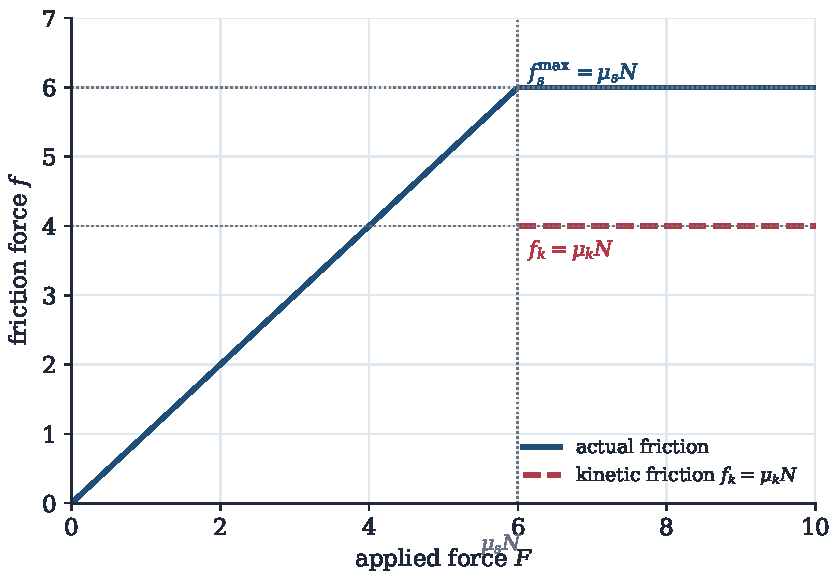
\includegraphics[width=0.78\textwidth]{figures/13_friction.pdf}
\caption{The friction force as a function of the applied force. The static
friction rises to $\mu_sN$; once sliding starts, the kinetic friction drops to
$\mu_kN$.}
\label{fig:friction}
\end{figure}

\begin{keyidea}[Angle of friction and angle of repose]
The maximum angle of an incline on which a body can rest without sliding is the
\emph{angle of repose}:
\[
\tan\alpha_c=\mu_s.
\]
For $\alpha<\alpha_c$, static friction can hold the body; for $\alpha>\alpha_c$,
it slides.
\end{keyidea}

\section{Rough inclined plane}

For a body sliding down a plane of angle $\alpha$ with kinetic friction,
\[
N=mg\cos\alpha,\qquad f_k=\mu_kN=\mu_kmg\cos\alpha,
\]
and along the plane
\[
ma=mg\sin\alpha-\mu_kmg\cos\alpha,
\]
so
\[
\boxed{a=g\left(\sin\alpha-\mu_k\cos\alpha\right).}
\]
If the body is pushed up the plane, friction reverses and
$a=-g(\sin\alpha+\mu_k\cos\alpha)$.

\section{Connected bodies and pulleys}

For an ideal (massless, frictionless) pulley, the tension is the same on both
sides of the string. The masses have the same magnitude of acceleration, possibly
in opposite directions. The method is always:
\begin{enumerate}[leftmargin=1.5em,itemsep=2pt]
  \item choose a positive direction of motion;
  \item write Newton's second law for each body separately;
  \item use the constraint (same string length) to relate accelerations;
  \item solve the resulting linear system.
\end{enumerate}

\begin{figure}[htbp]
\centering
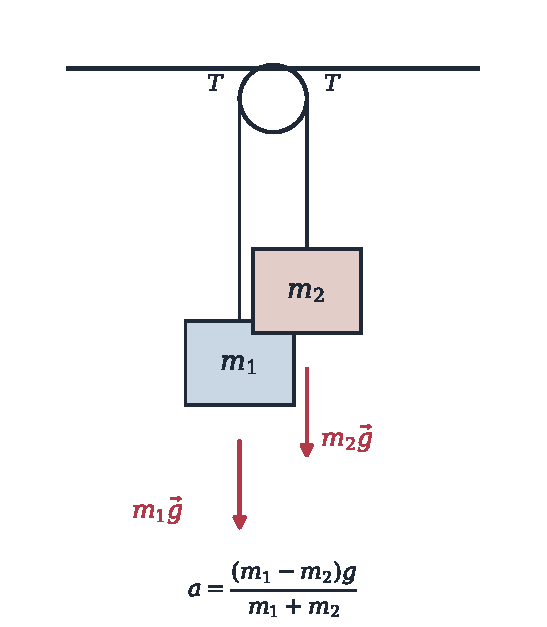
\includegraphics[width=0.52\textwidth]{figures/12_atwood.pdf}
\caption{The Atwood machine. The heavier mass descends; both masses have the same
magnitude of acceleration.}
\label{fig:atwood}
\end{figure}

\section{Elastic springs}

For an ideal spring of stiffness $k$ and natural length $l_0$,
\[
\vec F=-k(l-l_0)\,\vec u,
\]
where $\vec u$ points from the support to the free end. If $x=l-l_0$ is the
extension,
\[
F_x=-kx.
\]
At static equilibrium, the spring force balances the other forces.

\begin{figure}[htbp]
\centering
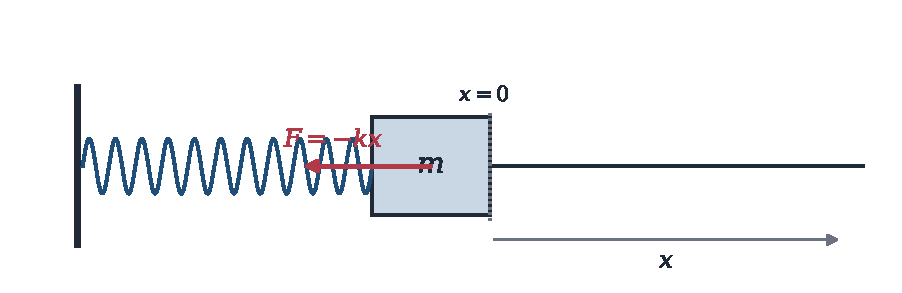
\includegraphics[width=0.82\textwidth]{figures/14_spring_mass.pdf}
\caption{A mass attached to a horizontal spring. The restoring force is
proportional to the displacement from equilibrium and points opposite to it.}
\label{fig:spring-mass}
\end{figure}

For springs in \textbf{series}, the same force acts on both and
\[
\frac1{k_{\mathrm{eq}}}=\frac1{k_1}+\frac1{k_2}.
\]
For springs in \textbf{parallel}, the extensions are equal and
\[
k_{\mathrm{eq}}=k_1+k_2.
\]

\section{Viscous drag and terminal velocity}

For slow motion in a fluid, a common model is
\[
\vec f=-k\vec v.
\]
A body falling from rest under gravity then obeys
\[
m\frac{\dd v}{\dd t}=mg-kv.
\]
The solution is
\[
v(t)=v_L\left(1-e^{-t/\tau}\right),
\qquad
v_L=\frac{mg}{k},\qquad
\tau=\frac mk.
\]
The velocity approaches the terminal velocity $v_L$ exponentially.

\begin{figure}[htbp]
\centering
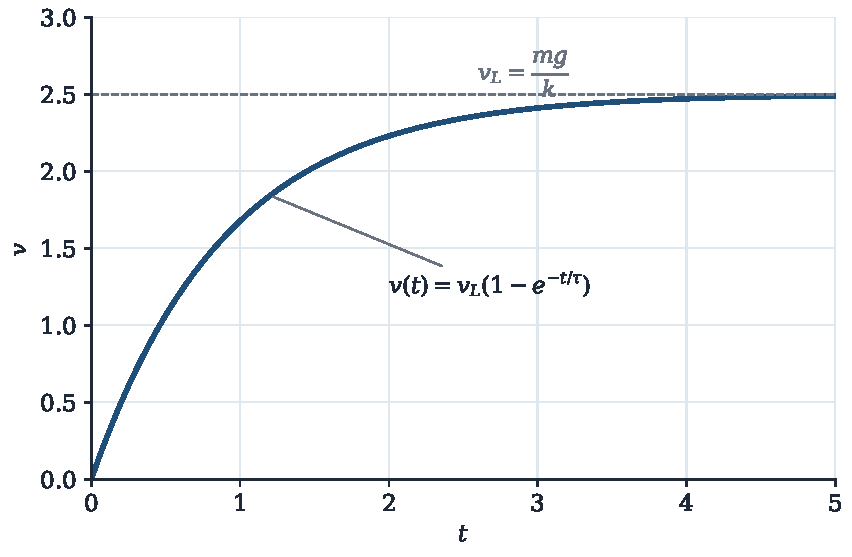
\includegraphics[width=0.72\textwidth]{figures/19_terminal_velocity.pdf}
\caption{Approach to terminal velocity for linear viscous drag.}
\label{fig:terminal}
\end{figure}

% ===========================================================================
\section{Worked examples}

\begin{worked}[Rough incline]
A block of mass $m=10.0\ \mathrm{kg}$ is placed on a plane inclined at
$\alpha=30.0^\circ$. The coefficients are $\mu_s=0.600$ and $\mu_k=0.250$.
(a) Does the block slide? (b) If it slides, find its acceleration.
\end{worked}

\begin{solution}{9.1}
The component of weight down the plane is
\[
mg\sin\alpha=10.0(9.81)\sin30.0^\circ=49.1\ \mathrm{N}.
\]
The normal reaction is
\[
N=mg\cos\alpha=10.0(9.81)\cos30.0^\circ=85.0\ \mathrm{N}.
\]
The maximum static friction is
\[
f_s^{\max}=\mu_sN=0.600(85.0)=51.0\ \mathrm{N}.
\]
Since $49.1<51.0$, the block does not slide.

If the block were already sliding, the kinetic friction would be
\[
f_k=\mu_kN=0.250(85.0)=21.3\ \mathrm{N},
\]
and the acceleration down the plane would be
\[
a=g(\sin\alpha-\mu_k\cos\alpha)
=9.81(0.500-0.250(0.866))=2.78\ \mathrm{m\,s^{-2}}.
\]
\end{solution}

\begin{worked}[Spring and mass]
A mass $m=0.500\ \mathrm{kg}$ is attached to a horizontal spring of stiffness
$k=200\ \mathrm{N\,m^{-1}}$ on a frictionless surface. The mass is pulled
$0.100\ \mathrm{m}$ from equilibrium and released.
(a) Find the spring force and acceleration at the instant of release.
(b) Find the acceleration when the mass passes through equilibrium.
\end{worked}

\begin{solution}{9.2}
(a) At release, $x=0.100\ \mathrm{m}$:
\[
F_x=-kx=-200(0.100)=-20.0\ \mathrm{N}.
\]
\[
a_x=\frac{F_x}{m}=\frac{-20.0}{0.500}=-40.0\ \mathrm{m\,s^{-2}}.
\]
The minus sign means the acceleration points back toward equilibrium.

(b) At equilibrium $x=0$, so $F_x=0$ and $a_x=0$. The velocity is maximum there.
\end{solution}

% ===========================================================================
\section{Exercises and Step-by-Step Solutions}

\begin{exercise}{\warm\ Starting a crate}
A crate of mass $50.0\ \mathrm{kg}$ rests on a horizontal floor. The coefficients
of friction are $\mu_s=0.500$ and $\mu_k=0.400$. Find the minimum horizontal force
needed to start the crate moving, and the force needed to keep it moving at
constant speed.
\end{exercise}

\begin{tabletworkspace}[6.5cm]
\end{tabletworkspace}

\begin{solution}{9.1}
\[
N=mg=50.0(9.81)=491\ \mathrm{N}.
\]
To start the motion:
\[
F_s=\mu_sN=0.500(491)=245\ \mathrm{N}.
\]
To keep it moving at constant speed:
\[
F_k=\mu_kN=0.400(491)=196\ \mathrm{N}.
\]
\end{solution}

\begin{exercise}{\warm\ Rough horizontal surface}
A $10.0\ \mathrm{kg}$ block is pulled horizontally by a force of
$50.0\ \mathrm{N}$ on a surface with $\mu_k=0.300$. Find its acceleration.
\end{exercise}

\begin{tabletworkspace}[6.5cm]
\end{tabletworkspace}

\begin{solution}{9.2}
\[
N=mg=10.0(9.81)=98.1\ \mathrm{N},\qquad
f_k=\mu_kN=0.300(98.1)=29.4\ \mathrm{N}.
\]
\[
a=\frac{F-f_k}{m}=\frac{50.0-29.4}{10.0}=2.06\ \mathrm{m\,s^{-2}}.
\]
\end{solution}

\begin{exercise}{\warm\ Spring extension}
A mass of $2.00\ \mathrm{kg}$ hangs from a vertical spring of stiffness
$k=300\ \mathrm{N\,m^{-1}}$. Find the extension at equilibrium and the force
needed to stretch the spring by $5.00\ \mathrm{cm}$.
\end{exercise}

\begin{tabletworkspace}[6.5cm]
\end{tabletworkspace}

\begin{solution}{9.3}
At equilibrium,
\[
kx=mg
\implies
x=\frac{mg}{k}=\frac{2.00(9.81)}{300}=0.0654\ \mathrm{m}.
\]
For a stretch $x=0.0500\ \mathrm{m}$,
\[
F=kx=300(0.0500)=15.0\ \mathrm{N}.
\]
\end{solution}

\begin{exercise}{\core\ Rough incline}
A block of mass $5.00\ \mathrm{kg}$ slides down a plane inclined at
$35.0^\circ$ with $\mu_k=0.200$. Find the normal reaction, the friction force,
and the acceleration.
\end{exercise}

\begin{tabletworkspace}[6.5cm]
\end{tabletworkspace}

\begin{solution}{9.4}
\[
N=mg\cos35.0^\circ=5.00(9.81)(0.8192)=40.2\ \mathrm{N}.
\]
\[
f_k=\mu_kN=0.200(40.2)=8.04\ \mathrm{N}.
\]
\[
a=g(\sin35.0^\circ-\mu_k\cos35.0^\circ)
=9.81(0.5736-0.1638)=4.02\ \mathrm{m\,s^{-2}}.
\]
\end{solution}

\begin{exercise}{\core\ Angle of repose}
The coefficient of static friction between a body and a plane is $\mu_s=0.450$.
Find the angle of repose. If the plane is inclined at $30.0^\circ$, does the body
slide?
\end{exercise}

\begin{tabletworkspace}[6.5cm]
\end{tabletworkspace}

\begin{solution}{9.5}
\[
\tan\alpha_c=\mu_s=0.450
\implies
\alpha_c=\arctan(0.450)=24.2^\circ.
\]
At $30.0^\circ>\alpha_c$, the body slides, because
$\tan30.0^\circ=0.577>0.450$.
\end{solution}

\begin{exercise}{\core\ Table, pulley, and friction}
A block $m_1=4.00\ \mathrm{kg}$ on a rough horizontal table
($\mu_k=0.250$) is connected by a string over a pulley to a hanging mass
$m_2=2.00\ \mathrm{kg}$. Find the acceleration and the tension.
\end{exercise}

\begin{tabletworkspace}[6.5cm]
\end{tabletworkspace}

\begin{solution}{9.6}
For $m_2$ (downward positive):
\[
m_2g-T=m_2a.
\]
For $m_1$:
\[
T-f_k=m_1a,\qquad f_k=\mu_km_1g.
\]
Adding,
\[
m_2g-\mu_km_1g=(m_1+m_2)a,
\]
\[
a=\frac{2.00(9.81)-0.250(4.00)(9.81)}{6.00}
=\frac{19.62-9.81}{6.00}=1.64\ \mathrm{m\,s^{-2}}.
\]
Then
\[
T=m_1(a+\mu_kg)=4.00(1.64+2.45)=16.4\ \mathrm{N}.
\]
\end{solution}

\begin{exercise}{\core\ Double incline}
Two masses $m_1=3.00\ \mathrm{kg}$ and $m_2=5.00\ \mathrm{kg}$ are connected by
a string over a pulley at the top of a double incline with angles
$\alpha=30.0^\circ$ for $m_1$ and $\beta=45.0^\circ$ for $m_2$. The surfaces are
frictionless. Find the acceleration and the tension.
\end{exercise}

\begin{tabletworkspace}[6.5cm]
\end{tabletworkspace}

\begin{solution}{9.7}
Assume $m_2$ slides down its plane and $m_1$ moves up its plane. For $m_1$:
\[
T-m_1g\sin\alpha=m_1a.
\]
For $m_2$:
\[
m_2g\sin\beta-T=m_2a.
\]
Adding,
\[
a=\frac{m_2g\sin\beta-m_1g\sin\alpha}{m_1+m_2}.
\]
\[
a=\frac{5.00(9.81)\sin45.0^\circ-3.00(9.81)\sin30.0^\circ}{8.00}
=\frac{34.68-14.72}{8.00}=2.50\ \mathrm{m\,s^{-2}}.
\]
\[
T=m_1(g\sin\alpha+a)=3.00(4.91+2.50)=22.2\ \mathrm{N}.
\]
\end{solution}

\begin{exercise}{\core\ Terminal velocity}
A body of mass $0.200\ \mathrm{kg}$ falls from rest subject to linear drag
$f=kv$ with $k=0.500\ \mathrm{kg\,s^{-1}}$. Find the terminal velocity, the time
constant, the speed at $t=1.20\ \mathrm{s}$, and the time to reach $99\%$ of the
terminal velocity.
\end{exercise}

\begin{tabletworkspace}[6.5cm]
\end{tabletworkspace}

\begin{solution}{9.8}
\[
v_L=\frac{mg}{k}=\frac{0.200(9.81)}{0.500}=3.92\ \mathrm{m\,s^{-1}},
\]
\[
\tau=\frac mk=\frac{0.200}{0.500}=0.400\ \mathrm{s}.
\]
At $t=1.20\ \mathrm{s}=3\tau$:
\[
v=3.92\left(1-e^{-3}\right)=3.92(0.950)=3.73\ \mathrm{m\,s^{-1}}.
\]
For $99\%$ of terminal velocity,
\[
1-e^{-t/\tau}=0.99
\implies
e^{-t/\tau}=0.01
\implies
t=\tau\ln100=0.400(4.605)=1.84\ \mathrm{s}.
\]
\end{solution}

\begin{exercise}{\mastery\ Springs in series and parallel}
Two springs of stiffness $k_1=100\ \mathrm{N\,m^{-1}}$ and
$k_2=200\ \mathrm{N\,m^{-1}}$ are combined. Find the equivalent stiffness
(a) in series and (b) in parallel. A mass of $2.00\ \mathrm{kg}$ hangs from each
combination; find the equilibrium extension in each case.
\end{exercise}

\begin{tabletworkspace}[6.5cm]
\end{tabletworkspace}

\begin{solution}{9.9}
(a) Series:
\[
\frac1{k_{\mathrm{eq}}}=\frac1{100}+\frac1{200}
=\frac{3}{200}
\implies
k_{\mathrm{eq}}=66.7\ \mathrm{N\,m^{-1}}.
\]
The extension under $m=2.00\ \mathrm{kg}$:
\[
x=\frac{mg}{k_{\mathrm{eq}}}=\frac{19.62}{66.7}=0.294\ \mathrm{m}.
\]

(b) Parallel:
\[
k_{\mathrm{eq}}=100+200=300\ \mathrm{N\,m^{-1}},
\]
\[
x=\frac{19.62}{300}=0.0654\ \mathrm{m}.
\]
\end{solution}

\begin{exercise}{\mastery\ Optimal pulling angle}
A block of mass $m$ is pulled on a rough horizontal floor by a force $F$ making
an angle $\theta$ above the horizontal. The coefficient of kinetic friction is
$\mu_k$.
(a) Show that
\[
a=\frac Fm(\cos\theta+\mu_k\sin\theta)-\mu_kg.
\]
(b) Show that the acceleration is maximum when $\tan\theta=\mu_k$.
(c) For $m=10.0\ \mathrm{kg}$, $F=50.0\ \mathrm{N}$, and $\mu_k=0.300$, compute
the optimal angle and the maximum acceleration.
\end{exercise}

\begin{tabletworkspace}[6.5cm]
\end{tabletworkspace}

\begin{solution}{9.10}
(a) The normal reaction is reduced by the vertical component of the pull:
\[
N=mg-F\sin\theta.
\]
The friction is $f_k=\mu_kN$, and the horizontal equation is
\[
ma=F\cos\theta-f_k=F\cos\theta-\mu_k(mg-F\sin\theta).
\]
Dividing by $m$,
\[
a=\frac Fm(\cos\theta+\mu_k\sin\theta)-\mu_kg.
\]

(b) Differentiate with respect to $\theta$:
\[
\frac{\dd a}{\dd\theta}=\frac Fm(-\sin\theta+\mu_k\cos\theta).
\]
Setting this to zero gives
\[
\tan\theta=\mu_k.
\]
The second derivative is negative at this point, so it is a maximum.

(c)
\[
\theta=\arctan(0.300)=16.7^\circ.
\]
\[
a_{\max}=\frac{50.0}{10.0}\left(\cos16.7^\circ+0.300\sin16.7^\circ\right)
-0.300(9.81).
\]
\[
a_{\max}=5.00(0.9578+0.0862)-2.943=5.22-2.94=2.28\ \mathrm{m\,s^{-2}}.
\]
\end{solution}


\chapter{Dynamics in Non-Inertial Reference Frames}
\label{ch:noninertial}
\begin{chapterintro}
\textbf{You will learn to:} distinguish inertial from non-inertial frames; compute the fictitious forces of transport and Coriolis; formulate Newton's second law in a moving frame; analyse apparent weight and the shape of rotating fluids; and calculate the eastward deflection of falling bodies and the precession of the Foucault pendulum.
\end{chapterintro}

\section{Inertial vs Non-Inertial Frames}

Newton's laws of motion are valid only in \textbf{inertial (Galilean) reference frames}---frames that are either at rest or moving at constant velocity with respect to the distant stars.

When we observe motion from an \textbf{accelerating or rotating reference frame} $\mathcal{R}'(O', x', y', z')$ relative to an inertial frame $\mathcal{R}(O, x, y, z)$, the frame itself experiences acceleration. To apply Newton's second law in $\mathcal{R}'$, we must introduce \textbf{fictitious (inertial) forces}. These forces do not arise from physical interactions (no physical agent pulls on the body), but are purely consequences of the acceleration of the observer's frame.

\begin{figure}[htbp]
\centering
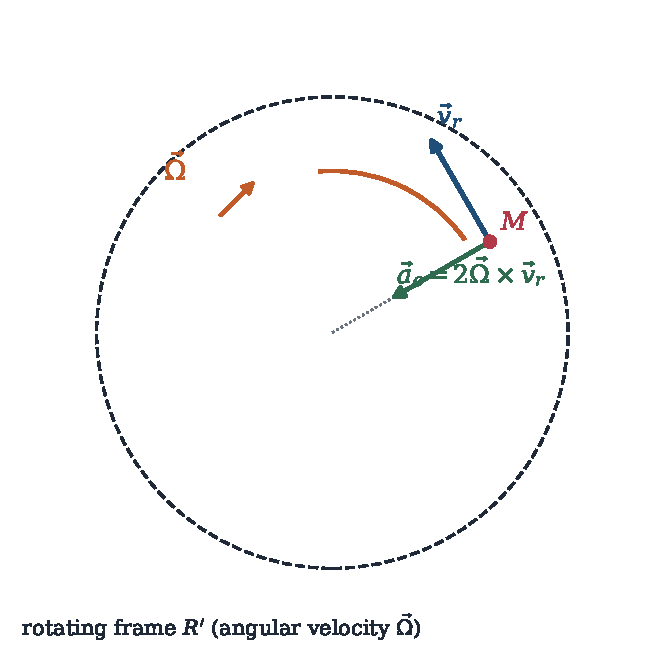
\includegraphics[width=0.72\textwidth]{figures/10_rotating_frame.pdf}
\caption{A particle $M$ observed from both a fixed inertial frame $\mathcal{R}(O,\ihat,\jhat,\khat)$ and a rotating frame $\mathcal{R}'(O',\ur,\ut,\khat)$ with angular velocity $\vec{\Omega}$.}
\label{fig:rotating_frame}
\end{figure}

\section{Composition of Accelerations and Fictitious Forces}

Recall from kinematics that the absolute acceleration $\vec{a}_a$ of a particle of mass $m$ is related to its relative acceleration $\vec{a}_r$ in $\mathcal{R}'$ by:
\[
\vec{a}_a = \vec{a}_r + \vec{a}_e + \vec{a}_c,
\]
where:
\begin{itemize}[leftmargin=1.4em,itemsep=3pt]
  \item $\vec{a}_r = \left(\frac{\dd^2\vec{r}'}{\dd t^2}\right)_{\mathcal{R}'}$ is the \textbf{relative acceleration} observed in $\mathcal{R}'$;
  \item $\vec{a}_e = \vec{a}(O') + \left(\frac{\dd\vec{\Omega}}{\dd t}\right)\times\vec{r}' + \vec{\Omega}\times(\vec{\Omega}\times\vec{r}')$ is the \textbf{acceleration of transport} (acceleration of the point in $\mathcal{R}'$ coincident with $M$);
  \item $\vec{a}_c = 2\vec{\Omega}\times\vec{v}_r$ is the \textbf{Coriolis acceleration}.
\end{itemize}

Multiplying by mass $m$ and using Newton's second law in the inertial frame, $m\vec{a}_a = \sum\vec{F}_{\text{real}}$, we obtain the \textbf{Fundamental Equation of Relative Dynamics}:
\[
\boxed{m\vec{a}_r = \sum\vec{F}_{\text{real}} + \vec{F}_{ie} + \vec{F}_{ic}}
\]
where the two inertial forces are:
\begin{align}
\vec{F}_{ie} &= -m\vec{a}_e \quad \text{(\textbf{Inertial force of transport / Centrifugal force})}, \\
\vec{F}_{ic} &= -m\vec{a}_c = -2m\,\vec{\Omega}\times\vec{v}_r \quad \text{(\textbf{Coriolis force})}.
\end{align}

\begin{keyidea}[Characteristics of Fictitious Forces]
\begin{itemize}[leftmargin=1.4em,itemsep=2pt]
  \item $\vec{F}_{ie}$ exists whenever the frame translates with acceleration ($\vec{a}(O')\ne\vzero$) or rotates. In a purely rotating frame ($\vec{\Omega} = \text{const}$, $O'=O$), $\vec{F}_{ie} = -m\vec{\Omega}\times(\vec{\Omega}\times\vec{r}') = m\Omega^2\vec{r}_\perp$ is directed \emph{radially outward} from the axis of rotation: the \textbf{centrifugal force}.
  \item $\vec{F}_{ic}$ acts \textbf{only when the particle is moving} in the relative frame ($\vec{v}_r\ne\vzero$). It is always perpendicular to the relative velocity ($\vec{F}_{ic}\cdot\vec{v}_r = 0$), meaning \textbf{the Coriolis force does no mechanical work} in the relative frame!
\end{itemize}
\end{keyidea}

\begin{method}[Solving Dynamics in a Non-Inertial Frame]
\begin{enumerate}[leftmargin=1.5em,itemsep=2pt]
  \item Identify the relative frame $\mathcal{R}'$ and its acceleration $\vec{a}(O')$ and angular velocity $\vec{\Omega}(t)$.
  \item Draw the free-body diagram of the particle including all \textbf{real forces} ($\vec{P}, \vec{N}, \vec{T}, \vec{f}$, etc.).
  \item Add the \textbf{fictitious forces}: $\vec{F}_{ie} = -m\vec{a}_e$ and $\vec{F}_{ic} = -2m\vec{\Omega}\times\vec{v}_r$.
  \item Apply $m\vec{a}_r = \sum\vec{F}_{\text{real}} + \vec{F}_{ie} + \vec{F}_{ic}$ along chosen coordinate axes in $\mathcal{R}'$.
\end{enumerate}
\end{method}

\section{Worked Examples}

\begin{worked}[Incline inside an accelerating truck]
A block of mass $m=2.0\ \mathrm{kg}$ sits on a smooth ramp of angle $\alpha=30^\circ$ fixed inside a truck. The truck accelerates horizontally with acceleration $a_0$. Find the acceleration $a_0$ such that the block remains at rest relative to the ramp.
\end{worked}

\begin{solution}{10.1}
In the frame of the truck $\mathcal{R}'$ (translating horizontally with $\vec{a}_0 = a_0\ihat$):
\begin{itemize}[leftmargin=1.4em,itemsep=2pt]
  \item Real forces: weight $\vec{P} = -mg\jhat$, normal force $\vec{N}$ perpendicular to the ramp ($N\sin\alpha\ihat + N\cos\alpha\jhat$).
  \item Fictitious force: $\vec{F}_{ie} = -m\vec{a}_0 = -m a_0\ihat$. Since $\vec{\Omega}=\vzero$, $\vec{F}_{ic}=\vzero$.
\end{itemize}
Relative equilibrium requires $\vec{a}_r = \vzero$, hence:
\[
\vec{P} + \vec{N} + \vec{F}_{ie} = \vzero.
\]
Projecting along the horizontal and vertical axes:
\begin{align*}
\text{Horizontal:}\quad & N\sin\alpha - m a_0 = 0 \implies N\sin\alpha = m a_0, \\
\text{Vertical:}\quad & N\cos\alpha - mg = 0 \implies N\cos\alpha = mg.
\end{align*}
Dividing the two equations eliminates $N$:
\[
\tan\alpha = \frac{a_0}{g} \implies \boxed{a_0 = g\tan\alpha.}
\]
For $\alpha=30^\circ$, $a_0 = 9.81\times\tan 30^\circ = 9.81\times 0.577 = 5.66\ \mathrm{m\,s^{-2}}$.
\end{solution}

\begin{worked}[Bead sliding on a rotating smooth rod]
A thin smooth horizontal rod rotates about a vertical axis through one end $O$ at constant angular velocity $\omega$. A bead of mass $m$ slides along the rod with distance $r(t)$ from $O$. Find the equation of motion for $r(t)$ and the horizontal reaction force exerted by the rod.
\end{worked}

\begin{solution}{10.2}
In the rotating frame $\mathcal{R}'$ attached to the rod with unit vector $\ur$ along the rod and $\ut$ perpendicular:
\begin{itemize}[leftmargin=1.4em,itemsep=2pt]
  \item The relative position is $\vec{r}' = r\ur$, relative velocity $\vec{v}_r = \dot{r}\ur$, relative acceleration $\vec{a}_r = \ddot{r}\ur$.
  \item Real forces: weight $\vec{P} = -mg\khat$, normal reaction $\vec{N} = N_\theta\ut + N_z\khat$ (since the rod is smooth, there is no component along $\ur$).
  \item Centrifugal force: $\vec{F}_{\text{cf}} = -m\vec{\Omega}\times(\vec{\Omega}\times\vec{r}') = m\omega^2 r\ur$.
  \item Coriolis force: $\vec{F}_{\text{Cor}} = -2m\vec{\Omega}\times\vec{v}_r = -2m(\omega\khat)\times(\dot{r}\ur) = -2m\omega\dot{r}\ut$.
\end{itemize}
Applying $m\vec{a}_r = \vec{P} + \vec{N} + \vec{F}_{\text{cf}} + \vec{F}_{\text{Cor}}$:
\begin{align*}
\ur:\quad & m\ddot{r} = m\omega^2 r \implies \boxed{\ddot{r} - \omega^2 r = 0,} \\
\ut:\quad & 0 = N_\theta - 2m\omega\dot{r} \implies \boxed{N_\theta = 2m\omega\dot{r},} \\
\khat:\quad & 0 = N_z - mg \implies N_z = mg.
\end{align*}
The radial equation $\ddot{r} - \omega^2 r = 0$ has solution $r(t) = A\cosh(\omega t) + B\sinh(\omega t)$. The bead accelerates exponentially outward! The rod must push horizontally with $N_\theta = 2m\omega\dot{r}$ to counteract the Coriolis force.
\end{solution}

\section{Exercises and Step-by-Step Solutions}

\begin{exercise}{\warm\ Scale in an accelerating elevator}
A student of mass $m=70.0\ \mathrm{kg}$ stands on a spring scale inside an elevator. What does the scale read (in newtons and equivalent apparent mass in $\mathrm{kg}$) when:
(a) the elevator accelerates upward at $a=2.00\ \mathrm{m\,s^{-2}}$;
(b) the elevator moves upward at constant speed $v=4.00\ \mathrm{m\,s^{-1}}$;
(c) the elevator accelerates downward at $a=2.00\ \mathrm{m\,s^{-2}}$;
(d) the elevator cable snaps and it falls freely?
\end{exercise}

\begin{tabletworkspace}[5.5cm]
\end{tabletworkspace}

\begin{solution}{10.1}
In the reference frame of the elevator $\mathcal{R}'$, the elevator has vertical acceleration $\vec{a} = a\jhat$ (with $\jhat$ upward).
The forces acting on the student in $\mathcal{R}'$ are:
\begin{itemize}[leftmargin=1.4em,itemsep=2pt]
  \item Real weight: $\vec{P} = -mg\jhat$;
  \item Normal reaction from the scale: $\vec{N} = N\jhat$ (the scale reads $N$);
  \item Fictitious inertial force: $\vec{F}_{ie} = -m\vec{a}_e = -m a\jhat$.
\end{itemize}
Since the student is at rest in the elevator ($\vec{a}_r = \vzero$):
\[
\vec{N} + \vec{P} + \vec{F}_{ie} = \vzero \implies N - mg - ma = 0 \implies N = m(g + a).
\]
(a) Accelerating upward ($a = +2.00\ \mathrm{m\,s^{-2}}$):
\[
N = 70.0(9.81 + 2.00) = 70.0(11.81) = 826.7\ \mathrm{N}.
\]
Apparent mass reading: $m_{\text{app}} = N/g = 826.7/9.81 = 84.3\ \mathrm{kg}$.

(b) Constant speed ($a = 0$):
\[
N = mg = 70.0\times 9.81 = 686.7\ \mathrm{N} \implies m_{\text{app}} = 70.0\ \mathrm{kg}.
\]

(c) Accelerating downward ($a = -2.00\ \mathrm{m\,s^{-2}}$):
\[
N = m(g - 2.00) = 70.0(9.81 - 2.00) = 70.0(7.81) = 546.7\ \mathrm{N} \implies m_{\text{app}} = 55.7\ \mathrm{kg}.
\]

(d) Free fall ($a = -g$):
\[
N = m(g - g) = 0\ \mathrm{N} \implies m_{\text{app}} = 0\ \mathrm{kg}\quad \text{(weightlessness)}.
\]
\end{solution}

\begin{exercise}{\warm\ Direction and magnitude of the Coriolis force}
A bullet of mass $m=20.0\ \mathrm{g}$ is fired horizontally due north at speed $v=800\ \mathrm{m\,s^{-1}}$ at a location in the Northern hemisphere with latitude $\lambda=45.0^\circ$.
(a) Determine the direction of the Coriolis force $\vec{F}_{\text{Cor}} = -2m\vec{\Omega}\times\vec{v}_r$.
(b) Calculate the magnitude of $\vec{F}_{\text{Cor}}$, given Earth's angular speed $\Omega \approx 7.292\times 10^{-5}\ \mathrm{rad\,s^{-1}}$.
(c) Compare this force with the bullet's weight $mg$.
\end{exercise}

\begin{tabletworkspace}[5.5cm]
\end{tabletworkspace}

\begin{solution}{10.2}
Set up a local coordinate frame with $\ihat$ pointing East, $\jhat$ pointing North, and $\khat$ pointing vertically upward (Zenith).
Earth's angular velocity vector $\vec{\Omega}$ points parallel to Earth's polar axis (North):
\[
\vec{\Omega} = \Omega\cos\lambda\jhat + \Omega\sin\lambda\khat.
\]
(a) The bullet flies horizontally due North: $\vec{v}_r = v\jhat$.
The cross product is:
\[
\vec{\Omega}\times\vec{v}_r = (\Omega\cos\lambda\jhat + \Omega\sin\lambda\khat)\times(v\jhat) = -\Omega v\sin\lambda\,\ihat.
\]
Therefore, the Coriolis force is:
\[
\vec{F}_{\text{Cor}} = -2m(\vec{\Omega}\times\vec{v}_r) = +2m\Omega v\sin\lambda\,\ihat.
\]
Since $\ihat$ is East, the Coriolis force is directed \textbf{due East} (deflecting the trajectory to the right).

(b) Magnitude:
\[
F_{\text{Cor}} = 2m\Omega v\sin\lambda = 2(0.0200)(7.292\times 10^{-5})(800)\sin 45^\circ = 2(0.0200)(7.292\times 10^{-5})(800)(0.7071) \approx 1.65\times 10^{-3}\ \mathrm{N}.
\]

(c) The weight is $P = mg = 0.0200\times 9.81 = 0.1962\ \mathrm{N}$.
The ratio is:
\[
\frac{F_{\text{Cor}}}{mg} = \frac{1.65\times 10^{-3}}{0.1962} \approx 8.4\times 10^{-3} \approx 0.84\%.
\]
Although small, over long trajectories (such as artillery shells or storm systems), this deflection is significant.
\end{solution}

\begin{exercise}{\core\ Plumb line deflection and apparent gravity}
Because the Earth rotates with angular speed $\Omega$ about its North-South axis, a plumb line does not point exactly toward the Earth's geometric center $O$.
(a) Show that the effective gravity $\vec{g}_{\text{eff}}$ at latitude $\lambda$ is given by $\vec{g}_{\text{eff}} = \vec{g}_0 + \Omega^2 R_E\cos\lambda\,\vec{u}_\perp$, where $\vec{g}_0 = -(GM_E/R_E^2)\vec{u}_r$ and $\vec{u}_\perp$ is directed perpendicular to the rotation axis outward.
(b) Find an expression for the deflection angle $\theta$ between the true vertical and the plumb line, assuming $\Omega^2 R_E \ll g_0$.
(c) Calculate the maximum deflection angle $\theta_{\max}$ and the latitude at which it occurs (take $R_E = 6.37\times 10^6\ \mathrm{m}$).
\end{exercise}

\begin{tabletworkspace}[6.0cm]
\end{tabletworkspace}

\begin{solution}{10.3}
(a) A plumb bob of mass $m$ hanging at rest relative to Earth ($\vec{v}_r = \vzero$) is in equilibrium under its true gravitational attraction $\vec{F}_g = m\vec{g}_0$, the string tension $\vec{T}$, and the centrifugal force $\vec{F}_{\text{cf}}$:
\[
\vec{T} + m\vec{g}_0 + \vec{F}_{\text{cf}} = \vzero.
\]
The apparent weight is defined as $\vec{P}_{\text{app}} = -\vec{T} = m\vec{g}_{\text{eff}}$. Thus:
\[
m\vec{g}_{\text{eff}} = m\vec{g}_0 + \vec{F}_{\text{cf}}.
\]
The distance from the bob to the rotation axis is $r_\perp = R_E\cos\lambda$. The centrifugal force is:
\[
\vec{F}_{\text{cf}} = m\Omega^2 r_\perp\vec{u}_\perp = m\Omega^2 R_E\cos\lambda\,\vec{u}_\perp.
\]
Dividing by $m$ yields:
\[
\vec{g}_{\text{eff}} = \vec{g}_0 + \Omega^2 R_E\cos\lambda\,\vec{u}_\perp.
\]

(b) Resolve $\vec{u}_\perp$ into local radial ($-\ur$, downward) and tangential ($\ut$, Southward) components:
\[
\vec{u}_\perp = \cos\lambda\,\ur - \sin\lambda\,\ut.
\]
Thus:
\begin{align*}
g_{\text{eff}, r} &= -g_0 + \Omega^2 R_E\cos^2\lambda \approx -g_0, \\
g_{\text{eff}, \theta} &= -\Omega^2 R_E\cos\lambda\sin\lambda = -\frac{1}{2}\Omega^2 R_E\sin(2\lambda).
\end{align*}
The deflection angle $\theta$ is small, so:
\[
\tan\theta \approx \theta \approx \frac{\abs{g_{\text{eff}, \theta}}}{\abs{g_{\text{eff}, r}}} \approx \frac{\Omega^2 R_E\sin(2\lambda)}{2g_0}.
\]

(c) The factor $\sin(2\lambda)$ reaches its maximum value of $1$ when $2\lambda = 90^\circ \implies \lambda = 45^\circ$.
At $\lambda = 45^\circ$:
\[
\theta_{\max} = \frac{\Omega^2 R_E}{2g_0} = \frac{(7.292\times 10^{-5})^2\times(6.37\times 10^6)}{2\times 9.81} = \frac{3.387\times 10^{-2}}{19.62} \approx 1.73\times 10^{-3}\ \mathrm{rad} \approx 0.099^\circ \approx 5.9'.
\]
The plumb line is deflected toward the equator by about $6$ arcminutes at $45^\circ$ latitude!
\end{solution}

\begin{exercise}{\core\ Liquid surface in an accelerating container}
A rectangular beaker of water is placed on a cart that accelerates horizontally with constant acceleration $a_0$ along the $+x$ direction.
(a) In the non-inertial frame of the beaker, determine the effective gravity $\vec{g}_{\text{eff}} = \vec{g} - \vec{a}_0$.
(b) Explain why the free surface of the liquid must be perpendicular to $\vec{g}_{\text{eff}}$.
(c) Deduce the angle of inclination $\theta$ of the liquid surface relative to the horizontal.
\end{exercise}

\begin{tabletworkspace}[5.5cm]
\end{tabletworkspace}

\begin{solution}{10.4}
(a) In the frame of the container $\mathcal{R}'$, each element of liquid experiences real gravity $\vec{g} = -g\jhat$ and the inertial force per unit mass $\vec{f}_{ie} = -\vec{a}_0 = -a_0\ihat$.
The effective gravitational acceleration in $\mathcal{R}'$ is:
\[
\vec{g}_{\text{eff}} = \vec{g} - \vec{a}_0 = -a_0\ihat - g\jhat.
\]

(b) At hydrostatic equilibrium in the relative frame, the pressure gradient satisfies $\vec{\nabla} p = \rho\vec{g}_{\text{eff}}$.
Along the free surface, the pressure is constant ($p = p_{\text{atm}}$), so $\dd p = \vec{\nabla} p\cdot\dd\vec{r} = 0$.
Therefore:
\[
\rho\vec{g}_{\text{eff}}\cdot\dd\vec{r} = 0 \implies \vec{g}_{\text{eff}}\perp\dd\vec{r}.
\]
The free surface must everywhere be orthogonal to the effective gravity vector $\vec{g}_{\text{eff}}$.

(c) Let the surface profile be $y(x)$. A tangent vector to the surface is $\dd\vec{r} = \dd x\ihat + \dd y\jhat$. The condition $\vec{g}_{\text{eff}}\cdot\dd\vec{r} = 0$ gives:
\[
(-a_0)\dd x + (-g)\dd y = 0 \implies \frac{\dd y}{\dd x} = -\frac{a_0}{g}.
\]
The surface is a flat plane tilted at an angle $\theta$ relative to the horizontal, with:
\[
\boxed{\tan\theta = \frac{a_0}{g}.}
\]
The liquid rises at the rear of the container and drops at the front.
\end{solution}

\begin{exercise}{\core\ Parabolic mirror: fluid in a rotating cylinder}
A cylindrical bucket containing liquid of density $\rho$ rotates about its central vertical axis at constant angular velocity $\omega$.
(a) Set up cylindrical coordinates $(r, \theta, z)$ in the rotating frame and find the effective force per unit volume on a fluid element.
(b) Integrate the hydrostatic equation $\vec{\nabla} p = \rho\vec{g}_{\text{eff}}$ to find the pressure distribution $p(r, z)$.
(c) Show that the free surface of the liquid forms a paraboloid of revolution, $z(r) = z_0 + \frac{\omega^2 r^2}{2g}$.
\end{exercise}

\begin{tabletworkspace}[6.0cm]
\end{tabletworkspace}

\begin{solution}{10.5}
(a) In the rotating frame $\mathcal{R}'$, the fluid is at rest. The forces per unit mass are gravity $\vec{g} = -g\khat$ and the centrifugal acceleration $\vec{a}_{\text{cf}} = \omega^2 r\ur$.
The effective field is:
\[
\vec{g}_{\text{eff}} = \omega^2 r\ur - g\khat.
\]
(Coriolis force is zero because $\vec{v}_r = \vzero$).

(b) Hydrostatic equilibrium in $\mathcal{R}'$:
\[
\vec{\nabla} p = \rho\vec{g}_{\text{eff}} \implies \frac{\partial p}{\partial r}\ur + \frac{1}{r}\frac{\partial p}{\partial \theta}\ut + \frac{\partial p}{\partial z}\khat = \rho\omega^2 r\ur - \rho g\khat.
\]
Matching components:
\[
\frac{\partial p}{\partial r} = \rho\omega^2 r,\qquad \frac{\partial p}{\partial \theta} = 0,\qquad \frac{\partial p}{\partial z} = -\rho g.
\]
Integrating:
\[
p(r, z) = p_0 + \frac{1}{2}\rho\omega^2 r^2 - \rho gz,
\]
where $p_0 = p(0, 0)$.

(c) Along the free surface, the pressure is atmospheric pressure $p_{\text{atm}}$. Setting $p(r, z) = p_{\text{atm}}$:
\[
p_{\text{atm}} = p_0 + \frac{1}{2}\rho\omega^2 r^2 - \rho gz \implies \rho gz = (p_0 - p_{\text{atm}}) + \frac{1}{2}\rho\omega^2 r^2.
\]
Defining $z_0 = z(0) = \frac{p_0 - p_{\text{atm}}}{\rho g}$:
\[
\boxed{z(r) = z_0 + \frac{\omega^2 r^2}{2g}.}
\]
This is a paraboloid of revolution! This principle is used in liquid-mirror astronomical telescopes (using molten gallium or mercury).
\end{solution}

\begin{exercise}{\core\ Mass on a rotating turntable with friction}
A small puck of mass $m=0.30\ \mathrm{kg}$ sits on a horizontal rotating turntable at a distance $r=0.25\ \mathrm{m}$ from the axis of rotation. The coefficient of static friction between puck and turntable is $\mu_s=0.40$.
(a) In the turntable frame, write the force balance condition for the puck to remain stationary.
(b) Calculate the maximum angular velocity $\omega_{\max}$ (in $\mathrm{rad\,s^{-1}}$ and in $\mathrm{rpm}$) before the puck slips.
(c) If the turntable rotates at $\omega = 5.0\ \mathrm{rad\,s^{-1}}$ and the puck is pushed radially inward with speed $v_r = 0.50\ \mathrm{m\,s^{-1}}$, compute the Coriolis force acting on it.
\end{exercise}

\begin{tabletworkspace}[5.5cm]
\end{tabletworkspace}

\begin{solution}{10.6}
(a) In the rotating frame of the turntable:
\begin{itemize}[leftmargin=1.4em,itemsep=2pt]
  \item Vertical: normal force $\vec{N} = N\khat$ balances weight $\vec{P} = -mg\khat \implies N = mg$.
  \item Horizontal: the centrifugal force $\vec{F}_{\text{cf}} = m\omega^2 r\ur$ pulls radially outward. To remain stationary ($\vec{v}_r = \vzero, \vec{a}_r = \vzero$), static friction $\vec{f}_s$ must point radially inward: $\vec{f}_s = -m\omega^2 r\ur$.
\end{itemize}
The condition for no slip is $f_s \le \mu_s N$:
\[
m\omega^2 r \le \mu_s mg \implies \omega^2 r \le \mu_s g.
\]

(b) Maximum angular velocity:
\[
\omega_{\max} = \sqrt{\frac{\mu_s g}{r}} = \sqrt{\frac{0.40\times 9.81}{0.25}} = \sqrt{15.696} \approx 3.96\ \mathrm{rad\,s^{-1}}.
\]
In revolutions per minute:
\[
N_{\text{rpm}} = \frac{\omega_{\max}\times 60}{2\pi} = \frac{3.96\times 60}{2\pi} \approx 37.8\ \mathrm{rpm}.
\]

(c) If the puck has relative velocity $\vec{v}_r = -v_r\ur$ (radially inward):
Earth's rotation vector is $\vec{\Omega} = \omega\khat$. The Coriolis force is:
\[
\vec{F}_{\text{Cor}} = -2m\vec{\Omega}\times\vec{v}_r = -2m(\omega\khat)\times(-v_r\ur) = +2m\omega v_r(\khat\times\ur) = 2m\omega v_r\ut.
\]
The Coriolis force pushes in the direction of rotation ($\ut$, forward tangential).
Magnitude:
\[
F_{\text{Cor}} = 2(0.30)(5.0)(0.50) = 1.50\ \mathrm{N}.
\]
\end{solution}

\begin{exercise}{\mastery\ Eastward deflection of a falling body}
A stone is dropped from rest from the top of a tower of height $h=100\ \mathrm{m}$ at latitude $\lambda=45^\circ$ in the Northern hemisphere.
(a) Using the coordinate system ($\ihat$ East, $\jhat$ North, $\khat$ Zenith), write the equations of motion for the stone in the Earth-bound frame including gravity and the Coriolis force (neglect the centrifugal term $\Omega^2 R_E$ and air resistance).
(b) By successive approximations (first-order in $\Omega$), show that the stone is deflected toward the East by an amount:
\[
d_E = \frac{1}{3}\Omega\cos\lambda\sqrt{\frac{8h^3}{g}}.
\]
(c) Calculate the numerical value of $d_E$.
\end{exercise}

\begin{tabletworkspace}[6.5cm]
\end{tabletworkspace}

\begin{solution}{10.7}
(a) In the local frame, $\vec{\Omega} = \Omega\cos\lambda\jhat + \Omega\sin\lambda\khat$.
The velocity is $\vec{v}_r = \dot{x}\ihat + \dot{y}\jhat + \dot{z}\khat$.
The Coriolis acceleration is:
\begin{align*}
\vec{a}_{\text{Cor}} &= -2\vec{\Omega}\times\vec{v}_r = -2\begin{vmatrix} \ihat & \jhat & \khat \\ 0 & \Omega\cos\lambda & \Omega\sin\lambda \\ \dot{x} & \dot{y} & \dot{z} \end{vmatrix} \\
&= -2\left[ (\dot{z}\Omega\cos\lambda - \dot{y}\Omega\sin\lambda)\ihat + (\dot{x}\Omega\sin\lambda)\jhat - (\dot{x}\Omega\cos\lambda)\khat \right].
\end{align*}
Newton's second law $m\vec{a}_r = m\vec{g} + \vec{F}_{\text{Cor}}$ yields the three scalar differential equations:
\begin{align*}
\ddot{x} &= 2\Omega(\dot{y}\sin\lambda - \dot{z}\cos\lambda), \\
\ddot{y} &= -2\Omega\dot{x}\sin\lambda, \\
\ddot{z} &= -g + 2\Omega\dot{x}\cos\lambda.
\end{align*}

(b) At zeroth order in $\Omega$ (unperturbed vertical fall with $x(0)=y(0)=0, z(0)=h$ and $\vec{v}(0)=\vzero$):
\[
\dot{x}^{(0)} = 0,\quad \dot{y}^{(0)} = 0,\quad \ddot{z}^{(0)} = -g \implies \dot{z}^{(0)}(t) = -gt,\quad z^{(0)}(t) = h - \frac{1}{2}gt^2.
\]
The fall time to ground level ($z=0$) is $t_f = \sqrt{2h/g}$.

Now substitute the zeroth-order solution into the $\ddot{x}$ equation to find the first-order correction:
\[
\ddot{x}^{(1)} = 2\Omega(0 - (-gt)\cos\lambda) = 2\Omega gt\cos\lambda.
\]
Integrating twice with initial conditions $x(0)=0, \dot{x}(0)=0$:
\begin{align*}
\dot{x}(t) &= \Omega gt^2\cos\lambda, \\
x(t) &= \frac{1}{3}\Omega gt^3\cos\lambda.
\end{align*}
Since $x$ is along the East axis, the deflection is strictly \textbf{Eastward}!
Evaluating at $t = t_f = \sqrt{2h/g}$:
\[
d_E = x(t_f) = \frac{1}{3}\Omega g \left(\frac{2h}{g}\right)^{3/2}\cos\lambda = \boxed{\frac{1}{3}\Omega\cos\lambda\sqrt{\frac{8h^3}{g}}.}
\]

(c) Numerical calculation with $h=100\ \mathrm{m}, g=9.81\ \mathrm{m\,s^{-2}}, \Omega=7.292\times 10^{-5}\ \mathrm{rad\,s^{-1}}, \lambda=45^\circ$:
\[
t_f = \sqrt{\frac{2\times 100}{9.81}} = \sqrt{20.387} \approx 4.515\ \mathrm{s}.
\]
\[
d_E = \frac{1}{3}(7.292\times 10^{-5})(9.81)(4.515)^3\cos 45^\circ \approx 0.0155\ \mathrm{m} = \mathbf{1.55\ \mathrm{cm}}.
\]
The stone lands $1.55\ \mathrm{cm}$ East of the point directly below its release point.
\end{solution}

\begin{exercise}{\mastery\ Bead on a rotating vertical hoop}
A smooth circular wire hoop of radius $R$ is placed in a vertical plane and rotates about its vertical diameter with constant angular speed $\omega$. A bead of mass $m$ slides without friction on the hoop. The position of the bead is specified by the angle $\theta$ from the lowest point.
(a) In the rotating frame of the hoop, identify all real and fictitious forces acting on the bead.
(b) Project the equation of motion along the tangent to the hoop to show:
\[
R\ddot{\theta} = \left(\omega^2 R\cos\theta - g\right)\sin\theta.
\]
(c) Find all equilibrium angles $\theta_e$ and determine their stability as a function of the rotation speed $\omega$, identifying the critical threshold $\omega_c = \sqrt{g/R}$.
\end{exercise}

\begin{tabletworkspace}[6.5cm]
\end{tabletworkspace}

\begin{solution}{10.8}
(a) In the frame $\mathcal{R}'$ rotating with $\vec{\Omega} = \omega\khat$:
\begin{itemize}[leftmargin=1.4em,itemsep=2pt]
  \item Real forces: weight $\vec{P} = -mg\khat$, normal reaction from the wire $\vec{N}$ (no component along the tangent $\vec{u}_\theta$ because the wire is smooth).
  \item Centrifugal force: $\vec{F}_{\text{cf}} = m\omega^2 r_\perp\ur = m\omega^2(R\sin\theta)\ur$, directed horizontally outward from the vertical axis.
  \item Coriolis force: perpendicular to $\vec{u}_\theta$ and absorbed by the normal reaction $\vec{N}$.
\end{itemize}

(b) Choose the tangential unit vector $\vec{u}_\theta$ along the hoop pointing in the direction of increasing $\theta$:
\begin{itemize}[leftmargin=1.4em,itemsep=2pt]
  \item Tangential component of weight: $P_\theta = -mg\sin\theta$.
  \item Tangential component of centrifugal force: $F_{\text{cf}, \theta} = +m\omega^2(R\sin\theta)\cos\theta = m\omega^2 R\sin\theta\cos\theta$.
\end{itemize}
Applying $m a_\theta = m R\ddot{\theta} = P_\theta + F_{\text{cf}, \theta}$:
\[
m R\ddot{\theta} = -mg\sin\theta + m\omega^2 R\sin\theta\cos\theta \implies \boxed{R\ddot{\theta} = \left(\omega^2 R\cos\theta - g\right)\sin\theta.}
\]

(c) Equilibria occur where $\ddot{\theta} = 0$:
\[
\sin\theta\left(\omega^2 R\cos\theta - g\right) = 0.
\]
This yields two possibilities:
\begin{enumerate}[leftmargin=1.4em,itemsep=2pt]
  \item $\sin\theta = 0 \implies \theta_1 = 0$ (lowest point) and $\theta_2 = \pi$ (highest point).
  \item $\omega^2 R\cos\theta - g = 0 \implies \cos\theta_3 = \frac{g}{\omega^2 R}$.
  Since $\abs{\cos\theta} \le 1$, this non-trivial equilibrium exists \textbf{if and only if} $\omega \ge \omega_c = \sqrt{g/R}$.
\end{enumerate}

\textbf{Stability analysis} via effective potential $V_{\text{eff}}(\theta)$:
Since $R\ddot{\theta} = -\frac{1}{mR}\frac{\dd V_{\text{eff}}}{\dd\theta}$:
\[
V_{\text{eff}}(\theta) = -mgR\cos\theta - \frac{1}{2}m\omega^2 R^2\sin^2\theta.
\]
Second derivative:
\[
\frac{\dd^2 V_{\text{eff}}}{\dd\theta^2} = mgR\cos\theta - m\omega^2 R^2\cos(2\theta).
\]
\begin{itemize}[leftmargin=1.4em,itemsep=2pt]
  \item At $\theta = 0$: $\left.\frac{\dd^2 V_{\text{eff}}}{\dd\theta^2}\right|_0 = mgR - m\omega^2 R^2 = mR(g - \omega^2 R)$.
  \begin{itemize}
    \item If $\omega < \omega_c$: positive, so $\theta = 0$ is \textbf{stable}.
    \item If $\omega > \omega_c$: negative, so $\theta = 0$ becomes \textbf{unstable}!
  \end{itemize}
  \item For $\omega > \omega_c$, the new equilibrium $\cos\theta_3 = \frac{g}{\omega^2 R}$ appears:
  \[
  \left.\frac{\dd^2 V_{\text{eff}}}{\dd\theta^2}\right|_{\theta_3} = m\omega^2 R^2\sin^2\theta_3 > 0.
  \]
  Thus, the off-axis positions $\pm\theta_3$ are \textbf{stable}! This is a classic supercritical pitchfork bifurcation.
\end{itemize}
\end{solution}

\begin{exercise}{\mastery\ The Foucault Pendulum}
A simple pendulum of length $L$ and bob mass $m$ is set up at latitude $\lambda$. For small oscillations ($z \approx 0, \dot{z} \approx 0$), the tension in the string is $T \approx mg$.
(a) In the horizontal plane $(x, y)$ ($x$ East, $y$ North), show that the equations of motion in the rotating Earth frame are:
\begin{align*}
\ddot{x} - 2\omega_z\dot{y} + \omega_0^2 x &= 0, \\
\ddot{y} + 2\omega_z\dot{x} + \omega_0^2 y &= 0,
\end{align*}
where $\omega_0 = \sqrt{g/L}$ and $\omega_z = \Omega\sin\lambda$.
(b) Introduce the complex coordinate $\eta(t) = x(t) + \mathrm{i}y(t)$ to combine these equations into:
\[
\ddot{\eta} + 2\mathrm{i}\omega_z\dot{\eta} + \omega_0^2\eta = 0.
\]
(c) Given $\omega_z \ll \omega_0$, solve for $\eta(t)$ with initial conditions $\eta(0) = x_0, \dot{\eta}(0) = 0$, and show that the plane of oscillation rotates with angular velocity $-\omega_z = -\Omega\sin\lambda$. What is the rotation period at the North Pole and at Paris ($\lambda = 48.8^\circ$)?
\end{exercise}

\begin{tabletworkspace}[6.5cm]
\end{tabletworkspace}

\begin{solution}{10.9}
(a) For small oscillations, the restoring force from the string tension has horizontal components:
\[
F_{x, \text{rest}} \approx -T\frac{x}{L} \approx -mg\frac{x}{L} = -m\omega_0^2 x,\qquad F_{y, \text{rest}} \approx -m\omega_0^2 y.
\]
The Coriolis force with $\vec{\Omega} = \Omega\cos\lambda\jhat + \Omega\sin\lambda\khat$ and $\vec{v}_r \approx \dot{x}\ihat + \dot{y}\jhat$ gives:
\[
\vec{F}_{\text{Cor}} = -2m\begin{vmatrix} \ihat & \jhat & \khat \\ 0 & \Omega\cos\lambda & \Omega\sin\lambda \\ \dot{x} & \dot{y} & 0 \end{vmatrix} = 2m(\Omega\sin\lambda\dot{y})\ihat - 2m(\Omega\sin\lambda\dot{x})\jhat + 2m(\Omega\cos\lambda\dot{x})\khat.
\]
Defining $\omega_z = \Omega\sin\lambda$, the horizontal equations of motion $m\ddot{x} = F_{x, \text{rest}} + F_{\text{Cor}, x}$ and $m\ddot{y} = F_{y, \text{rest}} + F_{\text{Cor}, y}$ become:
\begin{align*}
m\ddot{x} &= -m\omega_0^2 x + 2m\omega_z\dot{y} \implies \boxed{\ddot{x} - 2\omega_z\dot{y} + \omega_0^2 x = 0,} \\
m\ddot{y} &= -m\omega_0^2 y - 2m\omega_z\dot{x} \implies \boxed{\ddot{y} + 2\omega_z\dot{x} + \omega_0^2 y = 0.}
\end{align*}

(b) Multiply the second equation by $\mathrm{i}$ and add it to the first:
\[
(\ddot{x} + \mathrm{i}\ddot{y}) + 2\omega_z(\mathrm{i}\dot{x} - \dot{y}) + \omega_0^2(x + \mathrm{i}y) = 0.
\]
Notice that $\mathrm{i}\dot{x} - \dot{y} = \mathrm{i}(\dot{x} + \mathrm{i}\dot{y}) = \mathrm{i}\dot{\eta}$.
Thus:
\[
\boxed{\ddot{\eta} + 2\mathrm{i}\omega_z\dot{\eta} + \omega_0^2\eta = 0.}
\]

(c) Try a solution of the form $\eta(t) = e^{-\mathrm{i}\omega_z t} u(t)$. Substituting:
\[
\dot{\eta} = e^{-\mathrm{i}\omega_z t}(\dot{u} - \mathrm{i}\omega_z u),\qquad \ddot{\eta} = e^{-\mathrm{i}\omega_z t}(\ddot{u} - 2\mathrm{i}\omega_z\dot{u} - \omega_z^2 u).
\]
The middle cross-term cancels:
\[
e^{-\mathrm{i}\omega_z t}\left[ (\ddot{u} - 2\mathrm{i}\omega_z\dot{u} - \omega_z^2 u) + 2\mathrm{i}\omega_z(\dot{u} - \mathrm{i}\omega_z u) + \omega_0^2 u \right] = 0 \implies \ddot{u} + (\omega_0^2 + \omega_z^2)u = 0.
\]
Since $\omega_z \approx 10^{-5}\ \mathrm{rad\,s^{-1}} \ll \omega_0 \approx 1\ \mathrm{rad\,s^{-1}}$, $\omega_0^2 + \omega_z^2 \approx \omega_0^2$.
The solution for $u(t)$ with $u(0)=x_0, \dot{u}(0)=0$ is:
\[
u(t) = x_0\cos(\omega_0 t).
\]
Therefore:
\[
\boxed{\eta(t) = x_0\cos(\omega_0 t)\,e^{-\mathrm{i}\omega_z t}.}
\]
The term $x_0\cos(\omega_0 t)$ represents simple harmonic oscillation along a line, while the factor $e^{-\mathrm{i}\omega_z t} = \cos(\omega_z t) - \mathrm{i}\sin(\omega_z t)$ rotates this line of oscillation clockwise with angular velocity:
\[
\Omega_F = -\omega_z = -\Omega\sin\lambda.
\]
The period of a complete $360^\circ$ rotation is:
\[
T_F = \frac{2\pi}{\abs{\Omega_F}} = \frac{2\pi}{\Omega\sin\lambda} = \frac{24\ \mathrm{h}}{\sin\lambda}.
\]
\begin{itemize}[leftmargin=1.4em,itemsep=2pt]
  \item At the North Pole ($\lambda = 90^\circ$): $T_F = 24.0\ \mathrm{h}$.
  \item At Paris ($\lambda = 48.8^\circ$): $T_F = \frac{24}{\sin 48.8^\circ} \approx \frac{24}{0.7524} \approx 31.9\ \mathrm{h} \approx 31\ \mathrm{h}\ 54\ \mathrm{min}$.
  \item At the Equator ($\lambda = 0^\circ$): $T_F \to \infty$ (no precession).
\end{itemize}
\end{solution}

\begin{exercise}{\mastery\ Centrifugal force potential and geoid flattening}
Because of the centrifugal force, the Earth is not a perfect sphere but an oblate spheroid flattened at the poles.
(a) Show that the centrifugal force $\vec{F}_{\text{cf}} = m\Omega^2 r_\perp\ur$ derives from a potential energy $E_{p, \text{cf}} = -\frac{1}{2}m\Omega^2 r^2\cos^2\lambda$.
(b) The effective potential energy of a unit mass at Earth's surface is $V_{\text{eff}} = -\frac{GM_E}{r} - \frac{1}{2}\Omega^2 r^2\cos^2\lambda$. Since mean sea level is an equipotential surface of $V_{\text{eff}}$, equate $V_{\text{eff}}$ at the pole ($r=R_p, \lambda=90^\circ$) and at the equator ($r=R_e, \lambda=0^\circ$) to estimate the equatorial bulge $\Delta R = R_e - R_p$ in terms of $g, R_E, \Omega$.
(c) Compute $\Delta R$ numerically.
\end{exercise}

\begin{tabletworkspace}[6.0cm]
\end{tabletworkspace}

\begin{solution}{10.10}
(a) The centrifugal force in cylindrical coordinates is $\vec{F}_{\text{cf}} = m\Omega^2 r_\perp\vec{u}_\perp$.
We check that $\vec{\nabla}\times\vec{F}_{\text{cf}} = \vzero$, so it derives from a potential:
\[
\vec{F}_{\text{cf}} = -\vec{\nabla} E_{p, \text{cf}} \implies \dd E_{p, \text{cf}} = -\vec{F}_{\text{cf}}\cdot\dd\vec{r} = -m\Omega^2 r_\perp\dd r_\perp.
\]
Integrating with zero at the axis:
\[
E_{p, \text{cf}} = -\frac{1}{2}m\Omega^2 r_\perp^2 = -\frac{1}{2}m\Omega^2 r^2\cos^2\lambda.
\]

(b) The effective potential per unit mass is:
\[
V_{\text{eff}}(r, \lambda) = -\frac{GM_E}{r} - \frac{1}{2}\Omega^2 r^2\cos^2\lambda.
\]
Equating potentials:
\begin{align*}
\text{At pole ($\lambda = 90^\circ, r=R_p$):}\quad & V_{\text{eff}} = -\frac{GM_E}{R_p}, \\
\text{At equator ($\lambda = 0^\circ, r=R_e$):}\quad & V_{\text{eff}} = -\frac{GM_E}{R_e} - \frac{1}{2}\Omega^2 R_e^2.
\end{align*}
Setting them equal:
\[
-\frac{GM_E}{R_p} = -\frac{GM_E}{R_e} - \frac{1}{2}\Omega^2 R_e^2 \implies GM_E\left(\frac{1}{R_p} - \frac{1}{R_e}\right) = \frac{1}{2}\Omega^2 R_e^2.
\]
Since $R_e - R_p = \Delta R \ll R_E$:
\[
\frac{1}{R_p} - \frac{1}{R_e} = \frac{R_e - R_p}{R_p R_e} \approx \frac{\Delta R}{R_E^2}.
\]
Using $g \approx \frac{GM_E}{R_E^2}$:
\[
g\,\Delta R \approx \frac{1}{2}\Omega^2 R_E^2 \implies \boxed{\Delta R \approx \frac{\Omega^2 R_E^2}{2g}.}
\]

(c) Numerical calculation:
\[
\Delta R = \frac{(7.292\times 10^{-5})^2\times(6.37\times 10^6)^2}{2\times 9.81} \approx \frac{215770}{19.62} \approx 10997\ \mathrm{m} \approx \mathbf{11.0\ \mathrm{km}}.
\]
\end{solution}

\chapter{Angular Momentum and Central Forces}
\label{ch:angular_momentum}
\begin{chapterintro}
\textbf{You will learn to:} define and compute angular momentum and torque; apply the angular momentum theorem; understand why central forces conserve angular momentum; use polar coordinates and the law of areas (Kepler's second law); analyse orbits with the effective potential $U_{\text{eff}}(r)$; and master Kepler's laws, orbital transfers, and Binet's formulas.
\end{chapterintro}

\section{Angular Momentum and Torque}

For a material point of mass $m$, position $\vec{r} = \vec{OM}$, and velocity $\vec{v}$ relative to a fixed origin $O$ in an inertial frame:
\begin{itemize}[leftmargin=1.4em,itemsep=3pt]
  \item The \textbf{angular momentum} about $O$ is:
        \[
        \boxed{\vec{L}_O = \vec{r}\times\vec{p} = m\,\vec{r}\times\vec{v}.}
        \]
  \item The \textbf{moment of a force (torque)} $\vec{F}$ about $O$ is:
        \[
        \boxed{\vec{\tau}_O = \vec{r}\times\vec{F}.}
        \]
\end{itemize}

Differentiating $\vec{L}_O$ with respect to time:
\[
\frac{\dd\vec{L}_O}{\dd t} = \frac{\dd\vec{r}}{\dd t}\times(m\vec{v}) + \vec{r}\times\left(m\frac{\dd\vec{v}}{\dd t}\right) = \vec{v}\times(m\vec{v}) + \vec{r}\times\vec{F}.
\]
Since $\vec{v}\times\vec{v} = \vzero$, we obtain the \textbf{Angular Momentum Theorem}:
\[
\boxed{\frac{\dd\vec{L}_O}{\dd t} = \vec{\tau}_O = \vec{r}\times\vec{F}.}
\]

\begin{figure}[htbp]
\centering
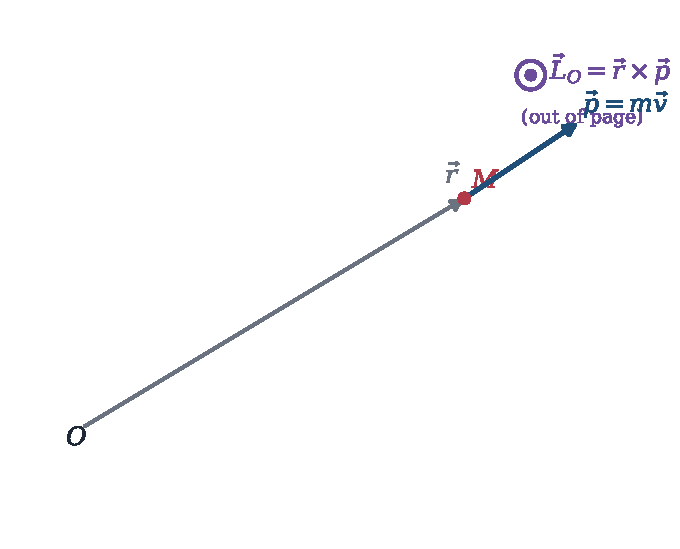
\includegraphics[width=0.72\textwidth]{figures/22_angular_momentum.pdf}
\caption{The position vector $\vec{r}$, linear momentum $\vec{p} = m\vec{v}$, and angular momentum vector $\vec{L}_O = \vec{r}\times\vec{p}$ perpendicular to the plane of motion.}
\label{fig:angular_momentum}
\end{figure}

\section{Central Forces and Conservation of Angular Momentum}

A force is called a \textbf{central force} with center $O$ if it is always directed along the line joining $O$ to the particle:
\[
\vec{F}(\vec{r}) = F(r)\,\ur, \quad \text{where } \ur = \frac{\vec{r}}{r}.
\]

\begin{keyidea}[Key Properties of Motion under a Central Force]
\begin{enumerate}[leftmargin=1.5em,itemsep=2pt]
  \item \textbf{Torque is identically zero}: $\vec{\tau}_O = \vec{r}\times(F(r)\ur) = \vzero$.
  \item \textbf{Angular momentum is strictly conserved}:
        \[
        \frac{\dd\vec{L}_O}{\dd t} = \vzero \implies \vec{L}_O = \vec{L}_0 = \text{constant vector}.
        \]
  \item \textbf{Planar trajectory}: Since $\vec{r}\cdot\vec{L}_0 = \vec{r}\cdot(\vec{r}\times\vec{p}) = 0$, the particle remains forever in the fixed plane passing through $O$ orthogonal to $\vec{L}_0$.
  \item \textbf{Constant areal velocity (Kepler's Second Law)}: In polar coordinates $(r, \theta)$ in the orbital plane:
        \[
        \vec{L}_O = m r\ur\times(\dot{r}\ur + r\dot{\theta}\ut) = m r^2\dot{\theta}\,\khat \implies \boxed{r^2\dot{\theta} = C = \frac{L_z}{m} = \text{constant},}
        \]
        where $C$ is the \emph{areal constant}. The rate at which area is swept out by the radius vector is:
        \[
        \frac{\dd A}{\dd t} = \frac{1}{2}r^2\dot{\theta} = \frac{C}{2} = \text{constant}.
        \]
\end{enumerate}
\end{keyidea}

\begin{figure}[htbp]
\centering
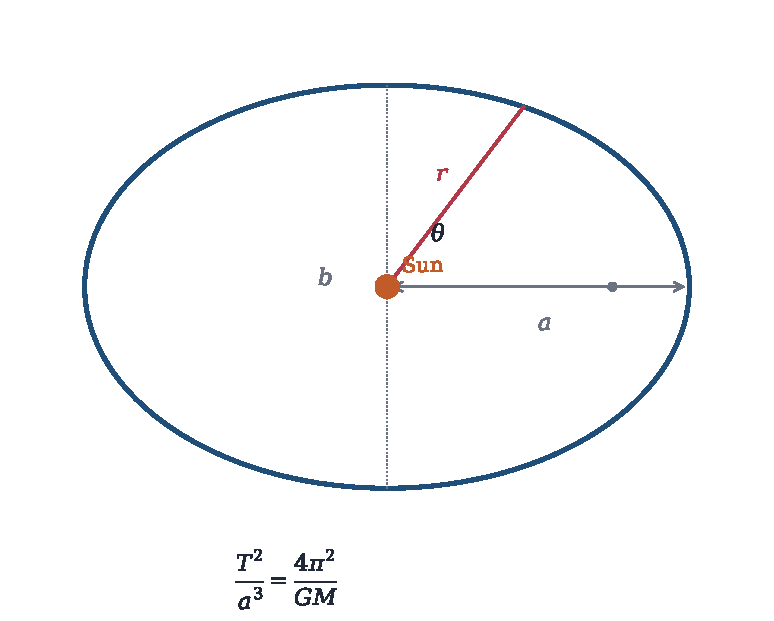
\includegraphics[width=0.74\textwidth]{figures/17_kepler.pdf}
\caption{An elliptical Keplerian orbit with the central body at one focus. Equal areas are swept out in equal times ($\Delta t_1 = \Delta t_2 \implies \Delta A_1 = \Delta A_2$).}
\label{fig:kepler_orbit}
\end{figure}

\section{The Effective Potential}

Since every central force $\vec{F} = F(r)\ur$ is conservative ($\vec{\nabla}\times\vec{F} = \vzero$), it possesses a potential energy $U(r)$ such that $F(r) = -\frac{\dd U}{\dd r}$.
The total mechanical energy in polar coordinates is:
\[
E_m = \frac{1}{2}m\left(\dot{r}^2 + r^2\dot{\theta}^2\right) + U(r).
\]
Substituting $r\dot{\theta} = \frac{L}{mr}$ reduces the 2D problem to an equivalent \textbf{one-dimensional radial motion}:
\[
\boxed{E_m = \frac{1}{2}m\dot{r}^2 + U_{\text{eff}}(r)}
\]
where the \textbf{effective potential} is:
\[
\boxed{U_{\text{eff}}(r) = U(r) + \frac{L^2}{2mr^2}.}
\]
The extra term $\frac{L^2}{2mr^2}$ is the \textbf{centrifugal barrier}, which prevents a particle with non-zero angular momentum from falling into the origin.

\section{Worked Examples}

\begin{worked}[Angular momentum of a projectile]
A projectile of mass $m$ is launched from the origin with initial velocity $\vec{v}_0 = v_0\cos\alpha\,\ihat + v_0\sin\alpha\,\jhat$ under gravity $\vec{g} = -g\jhat$.
(a) Find the angular momentum $\vec{L}_O(t)$ about the launch point $O$.
(b) Verify that $\frac{\dd\vec{L}_O}{\dd t} = \vec{\tau}_O(t)$.
\end{worked}

\begin{solution}{11.1}
(a) The position and velocity as functions of time are:
\[
\vec{r}(t) = (v_0\cos\alpha\,t)\ihat + \left(v_0\sin\alpha\,t - \frac{1}{2}gt^2\right)\jhat,
\]
\[
\vec{v}(t) = (v_0\cos\alpha)\ihat + (v_0\sin\alpha - gt)\jhat.
\]
The angular momentum about $O$ is:
\begin{align*}
\vec{L}_O(t) &= m\,\vec{r}\times\vec{v} = m\left[ x v_y - y v_x \right]\khat \\
&= m\left[ (v_0\cos\alpha\,t)(v_0\sin\alpha - gt) - \left(v_0\sin\alpha\,t - \frac{1}{2}gt^2\right)(v_0\cos\alpha) \right]\khat \\
&= m\left[ v_0^2\sin\alpha\cos\alpha\,t - g v_0\cos\alpha\,t^2 - v_0^2\sin\alpha\cos\alpha\,t + \frac{1}{2}g v_0\cos\alpha\,t^2 \right]\khat \\
&= \boxed{-\frac{1}{2}m g v_0\cos\alpha\,t^2\,\khat.}
\end{align*}

(b) The torque about $O$ due to gravity $\vec{P} = -mg\jhat$ is:
\[
\vec{\tau}_O = \vec{r}\times(-mg\jhat) = (x\ihat + y\jhat)\times(-mg\jhat) = -mgx\,\khat = -mg(v_0\cos\alpha\,t)\,\khat.
\]
Differentiating $\vec{L}_O(t)$:
\[
\frac{\dd\vec{L}_O}{\dd t} = \frac{\dd}{\dd t}\left(-\frac{1}{2}mgv_0\cos\alpha\,t^2\,\khat\right) = -mgv_0\cos\alpha\,t\,\khat = \vec{\tau}_O.
\]
The angular momentum theorem is verified!
\end{solution}

\begin{worked}[Perihelion and aphelion velocities in an elliptical orbit]
A satellite of mass $m$ orbits Earth (mass $M_E$) in an elliptical orbit. Its closest approach (perigee) is at distance $r_p$ and its farthest distance (apogee) is $r_a$. Express the speeds $v_p$ and $v_a$ in terms of $G, M_E, r_p, r_a$.
\end{worked}

\begin{solution}{11.2}
At both perigee and apogee, the velocity vector is perpendicular to the position vector ($\dot{r} = 0$).
\begin{itemize}[leftmargin=1.4em,itemsep=2pt]
  \item By conservation of angular momentum:
        \[
        L = m r_p v_p = m r_a v_a \implies v_a = \frac{r_p}{r_a}v_p.
        \]
  \item By conservation of mechanical energy:
        \[
        E_m = \frac{1}{2}mv_p^2 - \frac{GM_E m}{r_p} = \frac{1}{2}mv_a^2 - \frac{GM_E m}{r_a}.
        \]
\end{itemize}
Substituting $v_a = \frac{r_p}{r_a}v_p$:
\[
\frac{1}{2}v_p^2\left(1 - \frac{r_p^2}{r_a^2}\right) = GM_E\left(\frac{1}{r_p} - \frac{1}{r_a}\right) = GM_E\frac{r_a - r_p}{r_p r_a}.
\]
Notice that $1 - \frac{r_p^2}{r_a^2} = \frac{r_a^2 - r_p^2}{r_a^2} = \frac{(r_a - r_p)(r_a + r_p)}{r_a^2}$.
Cancelling the factor $(r_a - r_p)$:
\[
\frac{1}{2}v_p^2\frac{r_a + r_p}{r_a^2} = \frac{GM_E}{r_p r_a} \implies \boxed{v_p = \sqrt{\frac{2GM_E\,r_a}{r_p(r_p + r_a)}}.}
\]
By symmetry:
\[
\boxed{v_a = \sqrt{\frac{2GM_E\,r_p}{r_a(r_p + r_a)}}.}
\]
Since the semi-major axis is $a = \frac{r_p + r_a}{2}$, this can also be written in the famous \emph{vis-viva} form: $v^2 = GM_E\left(\frac{2}{r} - \frac{1}{a}\right)$.
\end{solution}

\section{Exercises and Step-by-Step Solutions}

\begin{exercise}{\warm\ Angular momentum in uniform rectilinear motion}
A particle of mass $m=0.50\ \mathrm{kg}$ travels at constant velocity $\vec{v} = 12.0\,\ihat\ \mathrm{m\,s^{-1}}$ along the line $y = 3.00\ \mathrm{m}$.
(a) Compute its angular momentum $\vec{L}_O$ about the origin $O(0,0)$ as a function of its $x$-coordinate.
(b) Does $\vec{L}_O$ depend on time or position? Explain why using the concept of torque.
\end{exercise}

\begin{tabletworkspace}[5.0cm]
\end{tabletworkspace}

\begin{solution}{11.1}
(a) The position vector is $\vec{r}(t) = x(t)\ihat + y_0\jhat$ with $y_0 = 3.00\ \mathrm{m}$.
The velocity is $\vec{v} = v_0\ihat$ with $v_0 = 12.0\ \mathrm{m\,s^{-1}}$.
The angular momentum about $O$ is:
\[
\vec{L}_O = \vec{r}\times(m\vec{v}) = (x\ihat + y_0\jhat)\times(m v_0\ihat) = -m v_0 y_0\,\khat.
\]
Substituting the numerical values:
\[
\vec{L}_O = -(0.50)(12.0)(3.00)\,\khat = \mathbf{-18.0\,\khat\ \mathrm{kg\,m^2\,s^{-1}}.}
\]

(b) $\vec{L}_O$ is strictly constant: it is completely independent of $x$ and $t$.
This is because the particle is in uniform rectilinear motion ($\vec{a} = \vzero$), so the net force is zero ($\vec{F} = \vzero$), meaning the net torque about the origin is $\vec{\tau}_O = \vec{r}\times\vec{F} = \vzero$. By the angular momentum theorem, $\frac{\dd\vec{L}_O}{\dd t} = \vzero$, so $\vec{L}_O = \text{const}$. Geometrically, $\norm{\vec{L}_O} = m v_0 d$, where $d = y_0$ is the perpendicular distance (impact parameter) from $O$ to the line of motion.
\end{solution}

\begin{exercise}{\warm\ Circular orbit speed and period of the ISS}
The International Space Station (ISS) orbits Earth in an approximately circular orbit at an altitude of $h = 415\ \mathrm{km}$ above Earth's surface.
(Earth's radius $R_E = 6371\ \mathrm{km}$, Earth's mass $M_E = 5.972\times 10^{24}\ \mathrm{kg}$, $G = 6.674\times 10^{-11}\ \mathrm{m^3\,kg^{-1}\,s^{-2}}$).
(a) Using Newton's second law, find the orbital speed $v_c$.
(b) Compute the orbital period $T$ in minutes.
(c) How many revolutions does the ISS complete in 24 hours?
\end{exercise}

\begin{tabletworkspace}[5.5cm]
\end{tabletworkspace}

\begin{solution}{11.2}
(a) The orbital radius is $r = R_E + h = 6371 + 415 = 6786\ \mathrm{km} = 6.786\times 10^6\ \mathrm{m}$.
For circular motion under gravity:
\[
m\frac{v_c^2}{r} = \frac{GM_E m}{r^2} \implies \boxed{v_c = \sqrt{\frac{GM_E}{r}}.}
\]
Computing:
\[
v_c = \sqrt{\frac{(6.674\times 10^{-11})(5.972\times 10^{24})}{6.786\times 10^6}} = \sqrt{\frac{3.986\times 10^{14}}{6.786\times 10^6}} = \sqrt{5.874\times 10^7} \approx 7664\ \mathrm{m\,s^{-1}} \approx \mathbf{7.66\ \mathrm{km\,s^{-1}}.}
\]

(b) The orbital period is:
\[
T = \frac{2\pi r}{v_c} = \frac{2\pi(6.786\times 10^6)}{7664} \approx 5563\ \mathrm{s} \approx \mathbf{92.7\ \mathrm{min}} \quad (1\ \mathrm{h}\ 32.7\ \mathrm{min}).
\]

(c) Number of orbits per day (24 hours = 1440 min):
\[
N = \frac{1440}{92.72} \approx \mathbf{15.5\ \text{orbits per day}}.
\]
\end{solution}

\begin{exercise}{\warm\ Escape velocity from celestial bodies}
The escape velocity $v_{\text{esc}}$ is the minimum speed needed for a projectile launched from the surface of a body to escape its gravitational pull completely ($r \to \infty$).
(a) Using conservation of mechanical energy, show that $v_{\text{esc}} = \sqrt{\frac{2GM}{R}} = \sqrt{2gR}$.
(b) Calculate $v_{\text{esc}}$ for Earth ($R_E = 6371\ \mathrm{km}, g = 9.81\ \mathrm{m\,s^{-2}}$).
(c) Calculate $v_{\text{esc}}$ for the Moon ($M_M = 7.342\times 10^{22}\ \mathrm{kg}, R_M = 1737\ \mathrm{km}$).
\end{exercise}

\begin{tabletworkspace}[5.0cm]
\end{tabletworkspace}

\begin{solution}{11.3}
(a) Mechanical energy at launch ($r = R$, $v = v_{\text{esc}}$):
\[
E_m = \frac{1}{2}m v_{\text{esc}}^2 - \frac{GMm}{R}.
\]
At infinity ($r \to \infty$), the gravitational potential energy vanishes ($U \to 0$), and the condition for just escaping is that the speed reaches zero ($v \ge 0$), so $E_{m, \infty} \ge 0$.
By conservation of energy:
\[
\frac{1}{2}m v_{\text{esc}}^2 - \frac{GMm}{R} = 0 \implies \boxed{v_{\text{esc}} = \sqrt{\frac{2GM}{R}}.}
\]
Since $g = \frac{GM}{R^2}$, we have $\frac{GM}{R} = gR$, so $v_{\text{esc}} = \sqrt{2gR}$.

(b) For Earth:
\[
v_{\text{esc}, E} = \sqrt{2(9.81)(6.371\times 10^6)} = \sqrt{1.250\times 10^8} \approx 11180\ \mathrm{m\,s^{-1}} = \mathbf{11.2\ \mathrm{km\,s^{-1}}.}
\]

(c) For the Moon:
\[
v_{\text{esc}, M} = \sqrt{\frac{2(6.674\times 10^{-11})(7.342\times 10^{22})}{1.737\times 10^6}} = \sqrt{\frac{9.800\times 10^{12}}{1.737\times 10^6}} = \sqrt{5.642\times 10^6} \approx 2375\ \mathrm{m\,s^{-1}} = \mathbf{2.38\ \mathrm{km\,s^{-1}}.}
\]
The Moon's escape velocity is nearly 5 times smaller than Earth's, which explains why the Moon could not retain an atmosphere.
\end{solution}

\begin{exercise}{\core\ Mass on a table with a hole: pulling the string}
A small puck of mass $m=0.20\ \mathrm{kg}$ on a frictionless horizontal table is connected to a light string passing through a small hole at the center $O$. The puck initially moves in a circle of radius $r_1 = 0.50\ \mathrm{m}$ with speed $v_1 = 2.0\ \mathrm{m\,s^{-1}}$. The string is then slowly pulled from below until the radius of the circular path is reduced to $r_2 = 0.25\ \mathrm{m}$.
(a) Explain why angular momentum about $O$ is conserved during the process.
(b) Find the new speed $v_2$ of the puck.
(c) Find the initial and final tension in the string.
(d) Calculate the work done by the person pulling the string using the work-energy theorem.
\end{exercise}

\begin{tabletworkspace}[6.0cm]
\end{tabletworkspace}

\begin{solution}{11.4}
(a) The string tension $\vec{T} = -T\ur$ is always directed toward the central hole $O$. The torque about $O$ is:
\[
\vec{\tau}_O = \vec{r}\times\vec{T} = r\ur\times(-T\ur) = \vzero.
\]
Therefore, angular momentum about $O$ is strictly conserved: $L = m r_1 v_1 = m r_2 v_2 = \text{const}$.

(b) Conserving angular momentum:
\[
v_2 = \frac{r_1}{r_2} v_1 = \frac{0.50}{0.25}\times 2.0 = 2\times 2.0 = \mathbf{4.0\ \mathrm{m\,s^{-1}}.}
\]

(c) The tension provides the centripetal acceleration $T = \frac{m v^2}{r}$:
\begin{align*}
T_1 &= \frac{m v_1^2}{r_1} = \frac{0.20\times (2.0)^2}{0.50} = \frac{0.80}{0.50} = \mathbf{1.60\ \mathrm{N},} \\
T_2 &= \frac{m v_2^2}{r_2} = \frac{0.20\times (4.0)^2}{0.25} = \frac{3.20}{0.25} = \mathbf{12.8\ \mathrm{N}.}
\end{align*}
The tension increases by a factor of $(r_1/r_2)^3 = 2^3 = 8$!

(d) By the work-energy theorem, since the normal force and gravity cancel and do no work, the work done by the tension force is the change in kinetic energy:
\[
W = \Delta E_c = \frac{1}{2}m v_2^2 - \frac{1}{2}m v_1^2 = \frac{1}{2}(0.20)\left[ 4.0^2 - 2.0^2 \right] = 0.10(16 - 4) = 0.10\times 12 = \mathbf{1.20\ \mathrm{J}.}
\]
The person pulling the string performs $+1.20\ \mathrm{J}$ of positive work against the centrifugal effect.
\end{solution}

\begin{exercise}{\core\ Effective potential and turning points}
A particle of mass $m$ moves under an attractive central force with potential $U(r) = -\frac{k}{r}$ ($k > 0$). Its angular momentum is $L$.
(a) Write down the effective potential $U_{\text{eff}}(r)$ and sketch it as a function of $r$.
(b) Find the radius $r_0$ of the circular orbit where $U_{\text{eff}}$ has its minimum, and compute the minimum energy $E_{\min} = U_{\text{eff}}(r_0)$.
(c) For total energy $E_m$ such that $E_{\min} < E_m < 0$, find the turning points $r_{\min}$ (periapsis) and $r_{\max}$ (apoapsis) in terms of $E_m, L, m, k$.
\end{exercise}

\begin{tabletworkspace}[6.5cm]
\end{tabletworkspace}

\begin{solution}{11.5}
(a) The effective potential is:
\[
\boxed{U_{\text{eff}}(r) = -\frac{k}{r} + \frac{L^2}{2mr^2}.}
\]
As $r \to 0$, the centrifugal term $\frac{L^2}{2mr^2} \to +\infty$ dominates (repulsive barrier).
As $r \to \infty$, $U_{\text{eff}}(r) \to 0^-$ (governed by $-\frac{k}{r}$).
In between, it exhibits a unique negative potential well minimum.

(b) The minimum occurs where $\frac{\dd U_{\text{eff}}}{\dd r} = 0$:
\[
\frac{\dd U_{\text{eff}}}{\dd r} = \frac{k}{r^2} - \frac{L^2}{mr^3} = 0 \implies \frac{k}{r_0^2} = \frac{L^2}{mr_0^3} \implies \boxed{r_0 = \frac{L^2}{mk}.}
\]
The second derivative is:
\[
\frac{\dd^2 U_{\text{eff}}}{\dd r^2} = -\frac{2k}{r^3} + \frac{3L^2}{mr^4} \implies \left.\frac{\dd^2 U_{\text{eff}}}{\dd r^2}\right|_{r_0} = -\frac{2k}{(L^2/mk)^3} + \frac{3L^2}{m(L^2/mk)^4} = \frac{m^3 k^4}{L^6} > 0,
\]
confirming a stable circular orbit!
The minimum energy is:
\[
E_{\min} = U_{\text{eff}}(r_0) = -\frac{k}{L^2/(mk)} + \frac{L^2}{2m(L^2/mk)^2} = -\frac{mk^2}{L^2} + \frac{mk^2}{2L^2} = \boxed{-\frac{mk^2}{2L^2}.}
\]

(c) Turning points are where the radial velocity vanishes: $\dot{r} = 0 \iff E_m = U_{\text{eff}}(r)$:
\[
E_m = -\frac{k}{r} + \frac{L^2}{2mr^2} \iff E_m r^2 + kr - \frac{L^2}{2m} = 0.
\]
Dividing by $E_m$ (with $E_m < 0$, let $\abs{E_m} = -E_m$):
\[
r^2 - \frac{k}{\abs{E_m}}r + \frac{L^2}{2m\abs{E_m}} = 0.
\]
Solving the quadratic equation:
\[
\Delta = \frac{k^2}{E_m^2} - \frac{2L^2}{m\abs{E_m}} = \frac{k^2}{E_m^2}\left(1 - \frac{2\abs{E_m}L^2}{mk^2}\right) = \frac{k^2}{E_m^2}\left(1 - \frac{\abs{E_m}}{\abs{E_{\min}}}\right).
\]
Since $E_{\min} < E_m < 0$, $\Delta > 0$. The two roots are:
\[
\boxed{r_{\min, \max} = \frac{k}{2\abs{E_m}}\left[ 1 \mp \sqrt{1 - \frac{2\abs{E_m}L^2}{mk^2}} \right].}
\]
Notice that the semi-major axis is $a = \frac{r_{\min} + r_{\max}}{2} = \frac{k}{2\abs{E_m}} \implies E_m = -\frac{k}{2a}$, and the eccentricity is $e = \sqrt{1 - \frac{2\abs{E_m}L^2}{mk^2}}$.
\end{solution}

\begin{exercise}{\core\ Hohmann Transfer Orbit to Mars}
A spacecraft is in a circular parking orbit around the Sun at Earth's distance $r_1 = 1.00\ \mathrm{AU} = 1.496\times 10^{11}\ \mathrm{m}$. It needs to transfer to Mars's orbit, assumed circular at $r_2 = 1.524\ \mathrm{AU} = 2.280\times 10^{11}\ \mathrm{m}$.
The Sun's gravitational parameter is $\mu = GM_\odot = 1.327\times 10^{20}\ \mathrm{m^3\,s^{-2}}$.
(a) Find the semi-major axis $a_{\text{trans}}$ of the elliptical Hohmann transfer orbit.
(b) Calculate the travel time (in days) to reach Mars.
(c) Compute the initial velocity increment $\Delta v_1$ required to leave Earth's orbit and enter the transfer ellipse.
\end{exercise}

\begin{tabletworkspace}[6.5cm]
\end{tabletworkspace}

\begin{solution}{11.6}
(a) The Hohmann transfer orbit is an ellipse with perihelion at Earth's orbit ($r_p = r_1$) and aphelion at Mars's orbit ($r_a = r_2$).
The major axis is $2a_{\text{trans}} = r_1 + r_2$, so:
\[
a_{\text{trans}} = \frac{r_1 + r_2}{2} = \frac{1.000 + 1.524}{2} = \mathbf{1.262\ \mathrm{AU}} = 1.262\times(1.496\times 10^{11}) = \mathbf{1.888\times 10^{11}\ \mathrm{m}.}
\]

(b) By Kepler's third law, the period of the complete ellipse is:
\[
T_{\text{trans}} = T_{\text{Earth}} \left(\frac{a_{\text{trans}}}{a_1}\right)^{3/2} = 1.00\ \text{year}\times(1.262)^{3/2} = 1.00\times 1.418 = 1.418\ \text{years}.
\]
The flight time to Mars is half of this orbital period (from perihelion to aphelion):
\[
t_{\text{flight}} = \frac{1}{2}T_{\text{trans}} = \frac{1.418\times 365.25}{2} \approx \mathbf{259\ \text{days}} \quad (\approx 8.5\ \text{months}).
\]

(c) Earth's circular orbital speed:
\[
v_{c1} = \sqrt{\frac{\mu}{r_1}} = \sqrt{\frac{1.327\times 10^{20}}{1.496\times 10^{11}}} \approx 29780\ \mathrm{m\,s^{-1}} = 29.78\ \mathrm{km\,s^{-1}}.
\]
The required perihelion speed on the transfer ellipse (using the \emph{vis-viva} equation $v^2 = \mu\left(\frac{2}{r} - \frac{1}{a}\right)$):
\[
v_{p} = \sqrt{\mu\left(\frac{2}{r_1} - \frac{1}{a_{\text{trans}}}\right)} = \sqrt{(1.327\times 10^{20})\left(\frac{2}{1.496\times 10^{11}} - \frac{1}{1.888\times 10^{11}}\right)} \approx 32730\ \mathrm{m\,s^{-1}} = 32.73\ \mathrm{km\,s^{-1}}.
\]
The required impulse at departure is:
\[
\Delta v_1 = v_p - v_{c1} = 32.73 - 29.78 = \mathbf{2.95\ \mathrm{km\,s^{-1}}.}
\]
\end{solution}

\begin{exercise}{\mastery\ Binet's Formulas and Kepler's First Law}
In polar coordinates $(r, \theta)$, define $u(\theta) = \frac{1}{r(\theta)}$.
(a) Using $r^2\dot{\theta} = C$, show that:
\[
\dot{r} = -C\frac{\dd u}{\dd\theta},\qquad \ddot{r} - r\dot{\theta}^2 = -C^2 u^2\left(\frac{\dd^2 u}{\dd\theta^2} + u\right).
\]
(b) Deduce \textbf{Binet's formula for acceleration}:
\[
a_r = -C^2 u^2\left(\frac{\dd^2 u}{\dd\theta^2} + u\right).
\]
(c) An observed orbit is an ellipse with the force center at one focus: $r(\theta) = \frac{p}{1 + e\cos\theta}$. Prove that the central force must be an inverse-square law $F(r) \propto -\frac{1}{r^2}$.
\end{exercise}

\begin{tabletworkspace}[6.5cm]
\end{tabletworkspace}

\begin{solution}{11.7}
(a) Using the chain rule $\frac{\dd}{\dd t} = \dot{\theta}\frac{\dd}{\dd\theta} = \frac{C}{r^2}\frac{\dd}{\dd\theta} = Cu^2\frac{\dd}{\dd\theta}$:
\[
\dot{r} = \frac{\dd}{\dd t}\left(\frac{1}{u}\right) = -\frac{1}{u^2}\dot{u} = -\frac{1}{u^2}\left(Cu^2\frac{\dd u}{\dd\theta}\right) = \boxed{-C\frac{\dd u}{\dd\theta}.}
\]
Differentiating again with respect to $t$:
\[
\ddot{r} = \frac{\dd}{\dd t}\left(-C\frac{\dd u}{\dd\theta}\right) = Cu^2\frac{\dd}{\dd\theta}\left(-C\frac{\dd u}{\dd\theta}\right) = -C^2 u^2\frac{\dd^2 u}{\dd\theta^2}.
\]
The second centripetal term is:
\[
r\dot{\theta}^2 = \frac{1}{u}\left(Cu^2\right)^2 = C^2 u^3.
\]
Combining the terms:
\[
\ddot{r} - r\dot{\theta}^2 = -C^2 u^2\frac{\dd^2 u}{\dd\theta^2} - C^2 u^3 = \boxed{-C^2 u^2\left(\frac{\dd^2 u}{\dd\theta^2} + u\right).}
\]

(b) In polar coordinates, the radial acceleration is precisely $a_r = \ddot{r} - r\dot{\theta}^2$. Therefore:
\[
\boxed{a_r = -C^2 u^2\left(\frac{\dd^2 u}{\dd\theta^2} + u\right).}
\]
Newton's second law $m a_r = F(r)$ gives Binet's equation:
\[
F(1/u) = -m C^2 u^2\left(\frac{\dd^2 u}{\dd\theta^2} + u\right).
\]

(c) Given the focal ellipse equation $r(\theta) = \frac{p}{1 + e\cos\theta}$:
\[
u(\theta) = \frac{1}{r(\theta)} = \frac{1}{p} + \frac{e}{p}\cos\theta.
\]
Differentiating twice with respect to $\theta$:
\[
\frac{\dd u}{\dd\theta} = -\frac{e}{p}\sin\theta,\qquad \frac{\dd^2 u}{\dd\theta^2} = -\frac{e}{p}\cos\theta.
\]
Adding $u$:
\[
\frac{\dd^2 u}{\dd\theta^2} + u = -\frac{e}{p}\cos\theta + \left(\frac{1}{p} + \frac{e}{p}\cos\theta\right) = \frac{1}{p} = \text{constant!}
\]
Substituting into Binet's force formula:
\[
F(r) = -m C^2 u^2\left(\frac{1}{p}\right) = -\frac{m C^2}{p} u^2 = \boxed{-\frac{m C^2}{p}\frac{1}{r^2}.}
\]
This completes Newton's celebrated deduction: an elliptical orbit with the focus at the center of force uniquely requires an \textbf{inverse-square gravitational force} $F(r) \propto -\frac{1}{r^2}$!
\end{solution}

\begin{exercise}{\mastery\ Rutherford Scattering: Repulsive Central Force}
An alpha particle of mass $m$ and charge $q_1 = +2e$ is fired with initial speed $v_0$ and impact parameter $b$ toward a stationary heavy gold nucleus of charge $q_2 = +Ze$.
The Coulomb repulsive force is $\vec{F} = \frac{k}{r^2}\ur$, where $k = \frac{q_1 q_2}{4\pi\varepsilon_0}$.
(a) Write the conservation of angular momentum $L$ and total mechanical energy $E_m$ in terms of $m, v_0, b$.
(b) Using Binet's equation $\frac{\dd^2 u}{\dd\theta^2} + u = -\frac{m k}{L^2}$, show that the trajectory is a hyperbola:
\[
u(\theta) = \frac{1}{r(\theta)} = \frac{1}{p}\left(e\cos\theta - 1\right),
\]
where $p = \frac{L^2}{mk}$.
(c) Deduce Rutherford's scattering formula relating the deflection angle $\theta_s$ to the impact parameter $b$:
\[
\tan\left(\frac{\theta_s}{2}\right) = \frac{k}{m v_0^2 b}.
\]
\end{exercise}

\begin{tabletworkspace}[6.5cm]
\end{tabletworkspace}

\begin{solution}{11.8}
(a) At $r \to \infty$, the particle moves with speed $v_0$ along a line at distance $b$ from the nucleus:
\[
L = m v_0 b = \text{const},\qquad E_m = \frac{1}{2}m v_0^2 = \text{const}.
\]

(b) Binet's equation for a repulsive force $F(r) = +\frac{k}{r^2} = +k u^2$:
\[
-m C^2 u^2\left(\frac{\dd^2 u}{\dd\theta^2} + u\right) = k u^2 \implies \frac{\dd^2 u}{\dd\theta^2} + u = -\frac{k}{m C^2} = -\frac{mk}{L^2}.
\]
Defining $p = \frac{L^2}{mk}$, this is a harmonic oscillator with constant drive:
\[
\frac{\dd^2 u}{\dd\theta^2} + u = -\frac{1}{p}.
\]
The general solution is:
\[
u(\theta) = A\cos(\theta - \theta_0) - \frac{1}{p}.
\]
Aligning the symmetry axis (periapsis at $\theta = 0$):
\[
u(\theta) = \frac{1}{p}\left(e\cos\theta - 1\right).
\]
Since $r > 0$, this represents the repulsive branch of a hyperbola ($e > 1$).

(c) The asymptotes of the hyperbola correspond to $r \to \infty \implies u(\theta_\infty) = 0$:
\[
e\cos\theta_\infty - 1 = 0 \implies \cos\theta_\infty = \frac{1}{e}.
\]
From the geometry of hyperbolic scattering, the incoming direction is $-\theta_\infty$ and the outgoing direction is $+\theta_\infty$.
The total deflection (scattering angle) is $\theta_s = \pi - 2\theta_\infty \implies \theta_\infty = \frac{\pi - \theta_s}{2}$.
Thus:
\[
\cos\theta_\infty = \cos\left(\frac{\pi}{2} - \frac{\theta_s}{2}\right) = \sin\left(\frac{\theta_s}{2}\right) = \frac{1}{e}.
\]
Consequently:
\[
\cot\left(\frac{\theta_s}{2}\right) = \sqrt{e^2 - 1}.
\]
To relate $e$ to $b$, note that at periapsis $r_0 = \frac{p}{e - 1}$, and using energy conservation $E_m = \frac{k(e^2 - 1)}{2p} = \frac{1}{2}m v_0^2$:
\[
e^2 - 1 = \frac{2 E_m p}{k} = \frac{2(\frac{1}{2}m v_0^2)(m^2 v_0^2 b^2 / mk)}{k} = \left(\frac{m v_0^2 b}{k}\right)^2.
\]
Taking the square root:
\[
\cot\left(\frac{\theta_s}{2}\right) = \frac{m v_0^2 b}{k} \implies \boxed{\tan\left(\frac{\theta_s}{2}\right) = \frac{k}{m v_0^2 b}.}
\]
This is the fundamental Rutherford scattering relation that revealed the atomic nucleus in 1911!
\end{solution}

\begin{exercise}{\mastery\ Distance of Closest Approach for an Alpha Particle}
In a head-on collision ($b = 0$), an alpha particle of mass $m = 6.64\times 10^{-27}\ \mathrm{kg}$ and kinetic energy $K = 5.00\ \mathrm{MeV}$ is fired directly at a gold nucleus ($Z = 79$).
($1\ \mathrm{eV} = 1.602\times 10^{-19}\ \mathrm{J}$, $\frac{1}{4\pi\varepsilon_0} = 8.988\times 10^9\ \mathrm{N\,m^2\,C^{-2}}$, $e = 1.602\times 10^{-19}\ \mathrm{C}$).
(a) Express the distance of closest approach $d_{\min}$ using conservation of energy.
(b) Calculate $d_{\min}$ in femtometres ($\mathrm{fm} = 10^{-15}\ \mathrm{m}$).
(c) What upper bound does this place on the radius of the gold nucleus?
\end{exercise}

\begin{tabletworkspace}[5.5cm]
\end{tabletworkspace}

\begin{solution}{11.9}
(a) For a head-on collision ($b = 0$), the particle travels along a straight line. At closest approach, its speed drops momentarily to zero ($v = 0$).
By conservation of mechanical energy:
\[
E_m = K_{\infty} = U(d_{\min}) \implies K = \frac{1}{4\pi\varepsilon_0}\frac{(2e)(Ze)}{d_{\min}} = \frac{2Ze^2}{4\pi\varepsilon_0\,d_{\min}}.
\]
Solving for $d_{\min}$:
\[
\boxed{d_{\min} = \frac{2Ze^2}{4\pi\varepsilon_0 K}.}
\]

(b) Convert $K = 5.00\ \mathrm{MeV}$ to joules:
\[
K = 5.00\times 10^6\times 1.602\times 10^{-19}\ \mathrm{J} = 8.01\times 10^{-13}\ \mathrm{J}.
\]
Calculate $d_{\min}$ with $Z = 79$:
\begin{align*}
d_{\min} &= \frac{(8.988\times 10^9)\times 2\times 79\times (1.602\times 10^{-19})^2}{8.01\times 10^{-13}} \\
&= \frac{(8.988\times 10^9)\times 158\times (2.566\times 10^{-38})}{8.01\times 10^{-13}} \\
&= \frac{3.644\times 10^{-26}}{8.01\times 10^{-13}} \approx 4.55\times 10^{-14}\ \mathrm{m} = \mathbf{45.5\ \mathrm{fm}.}
\end{align*}

(c) Because the alpha particle turns around purely under electrostatic repulsion without hitting the nuclear surface, the radius of the gold nucleus must be strictly less than $d_{\min}$:
\[
R_{\text{gold}} < 45.5\ \mathrm{fm}.
\]
(The actual measured nuclear radius of gold is $R \approx 1.2 A^{1/3} \approx 1.2(197)^{1/3} \approx 7.0\ \mathrm{fm}$).
\end{solution}

\begin{exercise}{\mastery\ Precession of the Perihelion under a Perturbed Central Force}
Consider a nearly circular planetary orbit under a modified gravitational potential $U(r) = -\frac{k}{r} - \frac{\epsilon}{r^2}$, where $\epsilon$ is a tiny relativistic correction.
(a) Find the effective potential $U_{\text{eff}}(r)$ and the radius $r_0$ of the circular orbit in terms of $L, m, k, \epsilon$.
(b) Perform a Taylor expansion of $U_{\text{eff}}(r)$ around $r_0$ to second order: $U_{\text{eff}}(r) \approx U_{\text{eff}}(r_0) + \frac{1}{2}k_{\text{eff}}(r - r_0)^2$. Find the radial oscillation frequency $\omega_r = \sqrt{k_{\text{eff}}/m}$.
(c) Comparing $\omega_r$ with the orbital angular frequency $\omega_\theta = \dot{\theta} = \frac{L}{m r_0^2}$, show that the perihelion precesses by an angle $\Delta\theta_p \approx \frac{2\pi\epsilon}{k r_0}$ per orbit.
\end{exercise}

\begin{tabletworkspace}[6.5cm]
\end{tabletworkspace}

\begin{solution}{11.10}
(a) The effective potential is:
\[
U_{\text{eff}}(r) = -\frac{k}{r} - \frac{\epsilon}{r^2} + \frac{L^2}{2mr^2} = -\frac{k}{r} + \frac{L^2 - 2m\epsilon}{2mr^2}.
\]
Define the modified angular momentum parameter $L'^2 = L^2 - 2m\epsilon$.
The circular orbit occurs at the minimum:
\[
\frac{\dd U_{\text{eff}}}{\dd r} = \frac{k}{r^2} - \frac{L'^2}{mr^3} = 0 \implies \boxed{r_0 = \frac{L'^2}{mk} \approx \frac{L^2}{mk}\left(1 - \frac{2m\epsilon}{L^2}\right).}
\]

(b) Second derivative at $r_0$:
\[
\frac{\dd^2 U_{\text{eff}}}{\dd r^2} = -\frac{2k}{r^3} + \frac{3L'^2}{mr^4}.
\]
Evaluating at $r_0 = \frac{L'^2}{mk}$:
\[
k_{\text{eff}} = \left.\frac{\dd^2 U_{\text{eff}}}{\dd r^2}\right|_{r_0} = -\frac{2k}{r_0^3} + \frac{3(mkr_0)}{mr_0^4} = \frac{k}{r_0^3}.
\]
The radial oscillation frequency is:
\[
\omega_r = \sqrt{\frac{k_{\text{eff}}}{m}} = \sqrt{\frac{k}{m r_0^3}}.
\]

(c) The orbital frequency for circular motion is $\omega_\theta = \frac{L}{m r_0^2}$.
Using $\frac{L^2}{m r_0^3} = \frac{L'^2 + 2m\epsilon}{m r_0^3} = \frac{m k r_0 + 2m\epsilon}{m r_0^3} = \frac{k}{r_0^2} + \frac{2\epsilon}{r_0^3}$:
\[
\omega_\theta = \sqrt{\frac{k}{m r_0^3} + \frac{2\epsilon}{m r_0^4}} = \omega_r \sqrt{1 + \frac{2\epsilon}{k r_0}} \approx \omega_r\left(1 + \frac{\epsilon}{k r_0}\right).
\]
The time between two consecutive perihelion passages is the radial period $T_r = \frac{2\pi}{\omega_r}$.
During this time, the polar angle increases by:
\[
\Delta\theta = \omega_\theta T_r = \omega_\theta \frac{2\pi}{\omega_r} \approx 2\pi\left(1 + \frac{\epsilon}{k r_0}\right) = 2\pi + \Delta\theta_p.
\]
Therefore, the perihelion advances each orbit by:
\[
\boxed{\Delta\theta_p \approx \frac{2\pi\epsilon}{k r_0}.}
\]
This orbital precession was precisely what Einstein used in 1915 to verify General Relativity through the 43 arcseconds per century anomalous precession of Mercury's perihelion!
\end{solution}


\part{Work and Energy}

\chapter{Work, Power, and the Work-Energy Theorem}
\label{ch:work_energy}
\begin{chapterintro}
\textbf{You will learn to:} define work as a line integral; calculate instantaneous and average power; apply the Work-Energy Theorem for particles; determine the work done by gravity, springs, and friction; and solve classic problems including vertical loops, detachment from surfaces, and resistive forces.
\end{chapterintro}

\section{Definition of Work}

When a force $\vec{F}$ acts on a material point undergoing an infinitesimal displacement $\dd\vec{r}$, the \textbf{elementary mechanical work} done by $\vec{F}$ is the scalar product:
\[
\boxed{\dd W = \vec{F}\cdot\dd\vec{r} = F_x\,\dd x + F_y\,\dd y + F_z\,\dd z = F\,\dd s\cos\theta,}
\]
where $\theta$ is the angle between $\vec{F}$ and the displacement tangent $\dd\vec{r}$, and $\dd s = \norm{\dd\vec{r}}$ is the arc length.

For a finite displacement along a curve $\mathcal{C}$ from initial point $A$ to final point $B$, the total work is the \textbf{line integral}:
\[
\boxed{W_{A\to B}(\vec{F}) = \int_{\mathcal{C}} \vec{F}\cdot\dd\vec{r}.}
\]
Work is measured in \textbf{joules} ($1\ \mathrm{J} = 1\ \mathrm{N\,m} = 1\ \mathrm{kg\,m^2\,s^{-2}}$).

\begin{figure}[htbp]
\centering
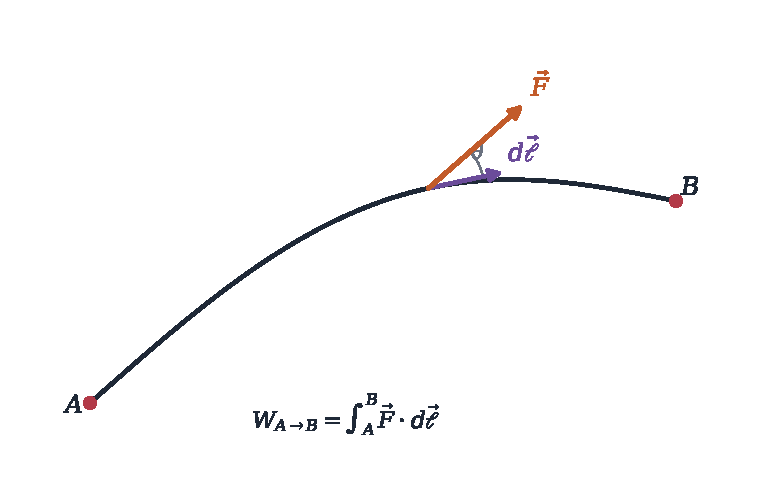
\includegraphics[width=0.74\textwidth]{figures/18_work_path.pdf}
\caption{The line integral of force $\vec{F}$ along a curved trajectory from point $A$ to point $B$. The tangential projection $F_t = \vec{F}\cdot\vec{u}_t$ contributes to the work.}
\label{fig:work_path}
\end{figure}

\begin{keyidea}[Sign of Mechanical Work]
\begin{itemize}[leftmargin=1.4em,itemsep=2pt]
  \item \textbf{Motive work} ($W > 0$): $\theta < 90^\circ$ ($\vec{F}\cdot\vec{v} > 0$). The force accelerates the particle, adding energy.
  \item \textbf{Resistive work} ($W < 0$): $\theta > 90^\circ$ ($\vec{F}\cdot\vec{v} < 0$). The force opposes motion, removing energy (e.g. friction).
  \item \textbf{Zero work} ($W = 0$): $\theta = 90^\circ$ ($\vec{F}\perp\vec{v}$). Forces perpendicular to velocity do \textbf{no work}!
  Examples: normal reactions from smooth rigid surfaces, magnetic forces ($\vec{F} = q\vec{v}\times\vec{B}$), and the Coriolis force ($\vec{F}_{ic} = -2m\vec{\Omega}\times\vec{v}_r$).
\end{itemize}
\end{keyidea}

\section{Instantaneous Power}

The rate at which work is performed with respect to time is the \textbf{instantaneous power}:
\[
\boxed{P(t) = \frac{\dd W}{\dd t} = \vec{F}\cdot\frac{\dd\vec{r}}{\dd t} = \vec{F}\cdot\vec{v}.}
\]
Power is measured in \textbf{watts} ($1\ \mathrm{W} = 1\ \mathrm{J\,s^{-1}} = 1\ \mathrm{kg\,m^2\,s^{-3}}$).

\section{The Work-Energy Theorem}

The \textbf{kinetic energy} of a material point of mass $m$ moving at speed $v$ is:
\[
\boxed{E_c = \frac{1}{2}m v^2 = \frac{p^2}{2m}.}
\]
Taking the time derivative of $E_c$:
\[
\frac{\dd E_c}{\dd t} = \frac{\dd}{\dd t}\left(\frac{1}{2}m\vec{v}\cdot\vec{v}\right) = m\vec{v}\cdot\frac{\dd\vec{v}}{\dd t} = \vec{v}\cdot(m\vec{a}) = \vec{v}\cdot\sum\vec{F} = P_{\text{net}}(t).
\]
Multiplying by $\dd t$:
\[
\dd E_c = \dd W_{\text{net}} = \sum\vec{F}\cdot\dd\vec{r}.
\]
Integrating between points $A$ and $B$ gives the \textbf{Work-Energy Theorem} (\emph{Théorème de l'énergie cinétique}):
\[
\boxed{\Delta E_c = E_c(B) - E_c(A) = \frac{1}{2}m v_B^2 - \frac{1}{2}m v_A^2 = W_{A\to B}\left(\sum\vec{F}\right).}
\]
\begin{keyidea}[Power of the Work-Energy Theorem]
The work-energy theorem allows us to find speeds directly from displacements \textbf{without needing to integrate Newton's second law with respect to time}!
\end{keyidea}

\section{Work Done by Common Forces}

\begin{center}
\renewcommand{\arraystretch}{1.3}
\begin{tabular}{@{}lll@{}}
\toprule
\textbf{Force} & \textbf{Expression} & \textbf{Work $W_{A\to B}$} \\
\midrule
Uniform gravity & $\vec{P} = -mg\khat$ & $-mg(z_B - z_A)$ \\
Ideal spring & $\vec{F}_s = -k x\ihat$ & $-\frac{1}{2}k(x_B^2 - x_A^2)$ \\
Kinetic friction & $\vec{f}_k = -\mu_k N\,\vec{u}_t$ & $-\int_A^B \mu_k N\,\dd s = -\mu_k N\,d$ (along straight line) \\
Normal reaction & $\vec{N}\perp\vec{v}$ & $0$ \\
\bottomrule
\end{tabular}
\end{center}

\section{Worked Examples}

\begin{worked}[Braking distance with kinetic friction]
A car travels at $v_0 = 90.0\ \mathrm{km\,h^{-1}} = 25.0\ \mathrm{m\,s^{-1}}$ on a horizontal road. The driver slams on the brakes, locking all four wheels. The coefficient of kinetic friction between tires and asphalt is $\mu_k = 0.700$. Using the work-energy theorem, find the stopping distance $d$.
\end{worked}

\begin{solution}{12.1}
The forces acting on the car during braking are:
\begin{itemize}[leftmargin=1.4em,itemsep=2pt]
  \item Vertical: gravity $\vec{P} = -mg\jhat$ and normal force $\vec{N} = N\jhat$. Since $a_y = 0$, $N = mg$.
  \item Horizontal: kinetic friction $\vec{f}_k = -\mu_k N\ihat = -\mu_k mg\ihat$.
\end{itemize}
Work done:
\begin{itemize}[leftmargin=1.4em,itemsep=2pt]
  \item $W(\vec{P}) = 0$ and $W(\vec{N}) = 0$ (perpendicular to displacement).
  \item $W(\vec{f}_k) = -f_k d = -\mu_k mg d$.
\end{itemize}
By the work-energy theorem between the initial state ($v_A = v_0$) and final stopped state ($v_B = 0$):
\[
\Delta E_c = 0 - \frac{1}{2}m v_0^2 = W_{\text{net}} = -\mu_k mg d.
\]
The mass $m$ cancels:
\[
\frac{1}{2}v_0^2 = \mu_k g d \implies \boxed{d = \frac{v_0^2}{2\mu_k g}.}
\]
Computing:
\[
d = \frac{(25.0)^2}{2(0.700)(9.81)} = \frac{625}{13.734} \approx \mathbf{45.5\ \mathrm{m}.}
\]
\end{solution}

\begin{worked}[The vertical loop-the-loop]
A small roller coaster car of mass $m$ starts from rest at height $h$ and slides down a frictionless track ending in a vertical circular loop of radius $R$.
(a) Find the speed of the car at the highest point of the loop (point $T$, at height $2R$).
(b) Find the normal force $N_T$ exerted by the track at the top.
(c) Deduce the minimum release height $h_{\min}$ to complete the loop without leaving the track.
\end{worked}

\begin{solution}{12.2}
(a) Applying the work-energy theorem between the release point $A$ (height $h$, $v_A = 0$) and the top of the loop $T$ (height $2R$, speed $v_T$):
Since the normal force $\vec{N}\perp\vec{v}$ does no work ($W(\vec{N}) = 0$), only gravity performs work:
\[
W_{A\to T}(\vec{P}) = -mg(z_T - z_A) = -mg(2R - h) = mg(h - 2R).
\]
Thus:
\[
\Delta E_c = \frac{1}{2}m v_T^2 - 0 = mg(h - 2R) \implies \boxed{v_T^2 = 2g(h - 2R).}
\]

(b) At point $T$, both gravity and the track normal force $\vec{N}_T$ point vertically downward toward the center of the circle:
\[
\sum F_{\text{rad}} = N_T + mg = m\frac{v_T^2}{R}.
\]
Solving for $N_T$:
\[
N_T = m\frac{v_T^2}{R} - mg = \frac{m}{R}\left[ 2g(h - 2R) \right] - mg = mg\left( \frac{2h}{R} - 5 \right).
\]

(c) The car remains on the track as long as the normal force is non-negative ($N_T \ge 0$):
\[
mg\left( \frac{2h}{R} - 5 \right) \ge 0 \implies \frac{2h}{R} \ge 5 \implies \boxed{h_{\min} = \frac{5}{2}R = 2.5R.}
\]
At this minimum height, the speed at the top is $v_T = \sqrt{gR}$, and the car is momentarily in free fall ($N_T = 0$).
\end{solution}

\section{Exercises and Step-by-Step Solutions}

\begin{exercise}{\warm\ Pulling a crate at an angle}
A worker pulls a crate of mass $m=40.0\ \mathrm{kg}$ across a smooth horizontal floor over a distance $d=15.0\ \mathrm{m}$ by applying a force of magnitude $F=120\ \mathrm{N}$ via a rope angled at $\alpha=30.0^\circ$ above the horizontal.
(a) Compute the work done by each force: the pulling force $\vec{F}$, gravity $\vec{P}$, and normal force $\vec{N}$.
(b) If the crate starts from rest, find its final speed $v_f$ using the work-energy theorem.
\end{exercise}

\begin{tabletworkspace}[5.0cm]
\end{tabletworkspace}

\begin{solution}{12.1}
(a) Work calculations:
\begin{itemize}[leftmargin=1.4em,itemsep=2pt]
  \item Pulling force: $W(\vec{F}) = F d\cos\alpha = (120)(15.0)\cos 30.0^\circ = 1800\times 0.8660 \approx \mathbf{1559\ \mathrm{J}} = 1.56\ \mathrm{kJ}$.
  \item Gravity: $\vec{P} = -mg\jhat$ is perpendicular to displacement $\dd\vec{r} = \dd x\ihat \implies W(\vec{P}) = \mathbf{0\ \mathrm{J}}$.
  \item Normal force: $\vec{N} = N\jhat \perp \dd\vec{r} \implies W(\vec{N}) = \mathbf{0\ \mathrm{J}}$.
\end{itemize}

(b) Total net work: $W_{\text{net}} = 1559\ \mathrm{J}$.
By the work-energy theorem:
\[
\Delta E_c = \frac{1}{2}m v_f^2 - 0 = W_{\text{net}} \implies v_f = \sqrt{\frac{2 W_{\text{net}}}{m}} = \sqrt{\frac{2\times 1559}{40.0}} = \sqrt{77.94} \approx \mathbf{8.83\ \mathrm{m\,s^{-1}}.}
\]
\end{solution}

\begin{exercise}{\warm\ Cruising power of an automobile}
A car of mass $m=1400\ \mathrm{kg}$ cruises at a constant speed of $v=108\ \mathrm{km\,h^{-1}} = 30.0\ \mathrm{m\,s^{-1}}$ on a flat horizontal highway. The total resistance force opposing its motion (aerodynamic drag plus rolling resistance) is $F_{\text{res}} = 650\ \mathrm{N}$.
(a) What driving force $F_{\text{engine}}$ must the engine deliver at constant speed?
(b) Calculate the mechanical power output $P$ delivered to the wheels in kilowatts and horsepower ($1\ \mathrm{hp} = 746\ \mathrm{W}$).
(c) If the car now climbs an uphill slope of grade $5.0\%$ ($\sin\alpha \approx 0.050$), what power is needed to maintain the same speed?
\end{exercise}

\begin{tabletworkspace}[5.5cm]
\end{tabletworkspace}

\begin{solution}{12.2}
(a) At constant speed, $\vec{a} = \vzero$, so $\sum\vec{F} = \vzero$:
\[
F_{\text{engine}} - F_{\text{res}} = 0 \implies F_{\text{engine}} = F_{\text{res}} = \mathbf{650\ \mathrm{N}.}
\]

(b) Mechanical power:
\[
P = F_{\text{engine}} v = (650\ \mathrm{N})(30.0\ \mathrm{m\,s^{-1}}) = 19500\ \mathrm{W} = \mathbf{19.5\ \mathrm{kW}.}
\]
In horsepower:
\[
P_{\text{hp}} = \frac{19500}{746} \approx \mathbf{26.1\ \mathrm{hp}.}
\]

(c) On the $5\%$ incline, gravity adds a component opposing motion: $P_\parallel = mg\sin\alpha$.
\[
P_\parallel = (1400)(9.81)(0.050) = 686.7\ \mathrm{N}.
\]
The new required engine thrust is:
\[
F_{\text{new}} = F_{\text{res}} + mg\sin\alpha = 650 + 686.7 = 1336.7\ \mathrm{N}.
\]
The required power is:
\[
P_{\text{climb}} = F_{\text{new}} v = (1336.7)(30.0) = 40101\ \mathrm{W} \approx \mathbf{40.1\ \mathrm{kW}} \approx \mathbf{53.8\ \mathrm{hp}.}
\]
The required power more than doubles to climb the incline!
\end{solution}

\begin{exercise}{\core\ Mass sliding down a rough ramp}
A block of mass $m=3.00\ \mathrm{kg}$ is released from rest at the top of a ramp inclined at $\theta=37.0^\circ$ of length $L=5.00\ \mathrm{m}$. The coefficient of kinetic friction is $\mu_k=0.250$.
(a) Calculate the work done by gravity $W_g$ as the block slides down the entire ramp.
(b) Calculate the work done by friction $W_f$.
(c) Using the work-energy theorem, find the speed of the block at the bottom of the ramp.
\end{exercise}

\begin{tabletworkspace}[5.5cm]
\end{tabletworkspace}

\begin{solution}{12.3}
(a) The vertical height difference is $h = L\sin\theta = 5.00\sin 37.0^\circ = 5.00(0.6018) = 3.009\ \mathrm{m}$.
Work done by gravity:
\[
W_g = +mgh = (3.00)(9.81)(3.009) \approx \mathbf{88.56\ \mathrm{J}.}
\]

(b) The normal force perpendicular to the ramp is $N = mg\cos\theta$.
The kinetic friction force is $f_k = \mu_k N = \mu_k mg\cos\theta$.
Since friction opposes displacement over length $L$:
\[
W_f = -f_k L = -\mu_k mg\cos\theta\,L = -(0.250)(3.00)(9.81)(\cos 37.0^\circ)(5.00) = -(0.250)(3.00)(9.81)(0.7986)(5.00) \approx \mathbf{-29.38\ \mathrm{J}.}
\]

(c) Net work:
\[
W_{\text{net}} = W_g + W_f = 88.56 - 29.38 = 59.18\ \mathrm{J}.
\]
By the work-energy theorem:
\[
\frac{1}{2}m v_f^2 - 0 = W_{\text{net}} \implies v_f = \sqrt{\frac{2 W_{\text{net}}}{m}} = \sqrt{\frac{2\times 59.18}{3.00}} = \sqrt{39.45} \approx \mathbf{6.28\ \mathrm{m\,s^{-1}}.}
\]
\end{solution}

\begin{exercise}{\core\ Vertical spring: maximum stretch}
A mass $m=1.50\ \mathrm{kg}$ is attached to an unstretched vertical spring of stiffness $k=120\ \mathrm{N\,m^{-1}}$ and released from rest.
(a) State all forces acting on the mass and express their work when the spring stretches by a distance $x$.
(b) Use the work-energy theorem to find the maximum extension $x_{\max}$ of the spring.
(c) Compare $x_{\max}$ with the static equilibrium extension $x_{\text{eq}}$. Explain why $x_{\max} = 2x_{\text{eq}}$.
\end{exercise}

\begin{tabletworkspace}[5.5cm]
\end{tabletworkspace}

\begin{solution}{12.4}
(a) Two forces act during the vertical descent by distance $x$:
\begin{itemize}[leftmargin=1.4em,itemsep=2pt]
  \item Gravity: downward displacement by $x \implies W_g = +mgx$.
  \item Spring restoring force: $F_s = -kx$ opposing extension $\implies W_s = -\int_0^x kx'\dd x' = -\frac{1}{2}kx^2$.
\end{itemize}

(b) At maximum extension $x_{\max}$, the mass momentarily comes to rest ($v = 0$):
\[
\Delta E_c = 0 - 0 = 0.
\]
By the work-energy theorem:
\[
W_{\text{net}} = W_g + W_s = mgx_{\max} - \frac{1}{2}kx_{\max}^2 = 0.
\]
Since $x_{\max} \ne 0$:
\[
mg - \frac{1}{2}kx_{\max} = 0 \implies \boxed{x_{\max} = \frac{2mg}{k}.}
\]
Computing:
\[
x_{\max} = \frac{2(1.50)(9.81)}{120} = \frac{29.43}{120} \approx \mathbf{0.245\ \mathrm{m}} = 24.5\ \mathrm{cm}.
\]

(c) At static equilibrium, the net force is zero:
\[
\sum F = mg - kx_{\text{eq}} = 0 \implies x_{\text{eq}} = \frac{mg}{k} = \frac{24.5}{2} = 12.25\ \mathrm{cm}.
\]
Therefore, $x_{\max} = 2x_{\text{eq}}$.
Because the system has no friction, the mass does not stop at equilibrium; when passing through $x_{\text{eq}}$, it has maximum kinetic energy! It overshoots equilibrium by exactly an equal distance $x_{\text{eq}}$, oscillating symmetrically between $x=0$ and $x=2x_{\text{eq}}$.
\end{solution}

\begin{exercise}{\core\ Path-dependent work: conservative vs non-conservative forces}
Consider the force field $\vec{F}(x, y) = y^2\,\ihat + 2xy\,\jhat$ and a second force field $\vec{G}(x, y) = y\,\ihat + 2x\,\jhat$.
(a) Compute the work done by each force along Path 1: straight line from $(0,0)$ to $(1,1)$ ($y = x$).
(b) Compute the work done by each force along Path 2: from $(0,0)$ along the $x$-axis to $(1,0)$, then vertically to $(1,1)$.
(c) State which force is conservative and compute $\vec{\nabla}\times\vec{F}$ and $\vec{\nabla}\times\vec{G}$.
\end{exercise}

\begin{tabletworkspace}[6.5cm]
\end{tabletworkspace}

\begin{solution}{12.5}
(a) Path 1 ($y = x \implies \dd y = \dd x$ from $x=0$ to $x=1$):
\begin{align*}
W_1(\vec{F}) &= \int_0^1 (x^2\,\dd x + 2x^2\,\dd x) = \int_0^1 3x^2\,\dd x = \left[ x^3 \right]_0^1 = \mathbf{1.0\ \mathrm{J}.} \\
W_1(\vec{G}) &= \int_0^1 (x\,\dd x + 2x\,\dd x) = \int_0^1 3x\,\dd x = \left[ \frac{3}{2}x^2 \right]_0^1 = \mathbf{1.5\ \mathrm{J}.}
\end{align*}

(b) Path 2: Segment A: $(0,0)\to(1,0)$ ($y=0, \dd y=0, x: 0\to 1$); Segment B: $(1,0)\to(1,1)$ ($x=1, \dd x=0, y: 0\to 1$):
For $\vec{F}$:
\begin{align*}
W_{2A}(\vec{F}) &= \int_0^1 0^2\,\dd x = 0, \\
W_{2B}(\vec{F}) &= \int_0^1 2(1)y\,\dd y = \left[ y^2 \right]_0^1 = 1.0\ \mathrm{J}. \\
W_2(\vec{F}) &= 0 + 1.0 = \mathbf{1.0\ \mathrm{J}.}
\end{align*}
For $\vec{G}$:
\begin{align*}
W_{2A}(\vec{G}) &= \int_0^1 0\,\dd x = 0, \\
W_{2B}(\vec{G}) &= \int_0^1 2(1)\,\dd y = \left[ 2y \right]_0^1 = 2.0\ \mathrm{J}. \\
W_2(\vec{G}) &= 0 + 2.0 = \mathbf{2.0\ \mathrm{J}.}
\end{align*}

(c) Evaluating curls:
\[
(\vec{\nabla}\times\vec{F})_z = \frac{\partial F_y}{\partial x} - \frac{\partial F_x}{\partial y} = \frac{\partial(2xy)}{\partial x} - \frac{\partial(y^2)}{\partial y} = 2y - 2y = 0 \implies \vec{F} \text{ is \textbf{conservative!}}
\]
Hence $W_1(\vec{F}) = W_2(\vec{F}) = 1.0\ \mathrm{J}$ (independent of path; $E_p(x, y) = -x y^2$).
For $\vec{G}$:
\[
(\vec{\nabla}\times\vec{G})_z = \frac{\partial G_y}{\partial x} - \frac{\partial G_x}{\partial y} = \frac{\partial(2x)}{\partial x} - \frac{\partial(y)}{\partial y} = 2 - 1 = 1 \ne 0 \implies \vec{G} \text{ is \textbf{non-conservative!}}
\]
Hence $W_1(\vec{G}) = 1.5\ \mathrm{J} \ne W_2(\vec{G}) = 2.0\ \mathrm{J}$ (path-dependent).
\end{solution}

\begin{exercise}{\core\ Bead sliding off a spherical dome: detachment angle}
A small ice cube of mass $m$ is placed at the top of a smooth frictionless spherical igloo of radius $R$. Given a negligible nudge, it begins to slide down the surface.
(a) Using the work-energy theorem, find the speed $v(\theta)$ as a function of the polar angle $\theta$ measured from the top.
(b) Write Newton's second law along the radial direction to find the normal force $N(\theta)$.
(c) Find the angle $\theta_{\text{det}}$ at which the cube leaves the surface of the sphere, and the height above the ground at detachment.
\end{exercise}

\begin{tabletworkspace}[6.0cm]
\end{tabletworkspace}

\begin{solution}{12.6}
(a) The initial height at $\theta = 0$ is $z_0 = R$. At angle $\theta$, the height is $z(\theta) = R\cos\theta$.
The normal force is perpendicular to velocity, so $W(\vec{N}) = 0$.
By the work-energy theorem:
\[
\Delta E_c = \frac{1}{2}m v^2 - 0 = W_g = mg(R - R\cos\theta) \implies \boxed{v^2(\theta) = 2gR(1 - \cos\theta).}
\]

(b) Along the inward radial direction toward the center of the sphere:
\[
mg\cos\theta - N = m\frac{v^2}{R}.
\]
Substituting $v^2(\theta)$:
\[
N(\theta) = mg\cos\theta - m\frac{2gR(1 - \cos\theta)}{R} = mg\cos\theta - 2mg(1 - \cos\theta) = \boxed{mg(3\cos\theta - 2).}
\]

(c) The cube loses contact with the surface when the normal reaction drops to zero ($N(\theta_{\text{det}}) = 0$):
\[
mg(3\cos\theta_{\text{det}} - 2) = 0 \implies \boxed{\cos\theta_{\text{det}} = \frac{2}{3}.}
\]
The angle of detachment is:
\[
\theta_{\text{det}} = \arccos(2/3) \approx \mathbf{48.2^\circ.}
\]
The height above ground at detachment is:
\[
z_{\text{det}} = R\cos\theta_{\text{det}} = \mathbf{\frac{2}{3}R.}
\]
The cube flies off into parabolic trajectory after dropping through one-third of the radius!
\end{solution}

\begin{exercise}{\mastery\ Velocity-dependent drag: distance to halve speed}
A motorboat of mass $m=600\ \mathrm{kg}$ cuts its engine when traveling at speed $v_0=20.0\ \mathrm{m\,s^{-1}}$. Water resistance exerts a quadratic drag force $F_d = -b v^2$ with drag constant $b = 15.0\ \mathrm{kg\,m^{-1}}$.
(a) Write the work-energy theorem in differential form $\dd E_c = \dd W$ and deduce a differential equation relating speed $v$ and position $x$.
(b) Integrate the equation to find the speed $v(x)$ as a function of the distance $x$ traveled since the engine was cut.
(c) Calculate the distance $d_{1/2}$ the boat travels before its speed is reduced to $v_0/2 = 10.0\ \mathrm{m\,s^{-1}}$.
\end{exercise}

\begin{tabletworkspace}[5.5cm]
\end{tabletworkspace}

\begin{solution}{12.7}
(a) The differential work-energy relation is:
\[
\dd E_c = \dd\left(\frac{1}{2}m v^2\right) = m v\,\dd v.
\]
The work done over distance $\dd x$ is:
\[
\dd W = F_d\,\dd x = -b v^2\,\dd x.
\]
Equating $\dd E_c = \dd W$:
\[
m v\,\dd v = -b v^2\,\dd x \implies m\frac{\dd v}{v} = -b\,\dd x.
\]

(b) Separating variables and integrating from $(x=0, v=v_0)$ to $(x, v)$:
\[
\int_{v_0}^v \frac{\dd v'}{v'} = -\frac{b}{m}\int_0^x \dd x' \implies \ln\left(\frac{v}{v_0}\right) = -\frac{b}{m}x.
\]
Exponentiating:
\[
\boxed{v(x) = v_0\,e^{-\frac{b}{m}x}.}
\]
The speed decreases exponentially with distance traveled!

(c) Setting $v = v_0/2$:
\[
\frac{1}{2} = e^{-\frac{b}{m}d_{1/2}} \implies \frac{b}{m}d_{1/2} = \ln 2 \implies \boxed{d_{1/2} = \frac{m\ln 2}{b}.}
\]
Computing:
\[
d_{1/2} = \frac{(600)(0.69315)}{15.0} = 40.0\times 0.69315 \approx \mathbf{27.7\ \mathrm{m}.}
\]
\end{solution}

\begin{exercise}{\mastery\ Power delivered in lifting a heavy chain}
A heavy flexible uniform chain of total length $L$ and total mass $M$ (linear mass density $\lambda = M/L$) rests coiled on the floor. A crane lifts one end vertically at a constant speed $v_0$.
(a) At the instant when a length $y$ of the chain is off the ground, find the total upward force $F(t)$ that the crane must exert.
(Hint: consider both the weight of the suspended portion and the rate of change of momentum of each incoming link $\frac{\dd p}{\dd t} = \lambda v_0^2$).
(b) Compute the instantaneous power $P(t) = F(t)v_0$ delivered by the crane.
(c) Integrate $P(t)$ to find the total work $W_{\text{crane}}$ done to lift the entire chain ($y = L$).
(d) Compare $W_{\text{crane}}$ with the final mechanical energy $E_{m} = E_c + E_p$ of the suspended chain. Account for the difference.
\end{exercise}

\begin{tabletworkspace}[6.5cm]
\end{tabletworkspace}

\begin{solution}{12.8}
(a) Let a length $y$ be in the air moving at speed $v_0$.
In an infinitesimal time interval $\dd t$, a mass element $\dd m = \lambda\,\dd y = \lambda v_0\dd t$ at rest on the floor is abruptly jerked into motion at speed $v_0$.
The momentum acquired is $\dd p = (\dd m)v_0 = \lambda v_0^2\dd t$.
The required impulse force is $\frac{\dd p}{\dd t} = \lambda v_0^2$.
In addition, the crane must support the weight of the suspended segment, $P(y) = (\lambda y)g$.
Thus, the total lifting force is:
\[
\boxed{F(t) = \lambda g y + \lambda v_0^2 = \lambda\left(gy + v_0^2\right).}
\]

(b) The instantaneous power delivered by the crane is:
\[
\boxed{P(t) = F(t)v_0 = \lambda v_0\left(gy + v_0^2\right) = \lambda g y v_0 + \lambda v_0^3.}
\]

(c) The work done by the crane as $y$ goes from $0$ to $L$ (with $\dd y = v_0\dd t$):
\[
W_{\text{crane}} = \int_0^{L/v_0} P(t)\dd t = \int_0^L F(y)\dd y = \int_0^L (\lambda g y + \lambda v_0^2)\dd y = \frac{1}{2}\lambda g L^2 + \lambda v_0^2 L.
\]
Using $\lambda L = M$:
\[
\boxed{W_{\text{crane}} = \frac{1}{2}MgL + Mv_0^2.}
\]

(d) The mechanical energy of the fully lifted chain is:
\begin{itemize}[leftmargin=1.4em,itemsep=2pt]
  \item Kinetic energy: $E_c = \frac{1}{2}Mv_0^2$;
  \item Potential energy (center of mass is at $h_{CM} = L/2$): $E_p = Mg\frac{L}{2} = \frac{1}{2}MgL$.
\end{itemize}
Total final mechanical energy:
\[
E_m = \frac{1}{2}MgL + \frac{1}{2}Mv_0^2.
\]
The difference between the work supplied and the final mechanical energy is:
\[
W_{\text{crane}} - E_m = \left(\frac{1}{2}MgL + Mv_0^2\right) - \left(\frac{1}{2}MgL + \frac{1}{2}Mv_0^2\right) = \mathbf{\frac{1}{2}Mv_0^2.}
\]
This remaining half of the kinetic energy supplied ($\frac{1}{2}Mv_0^2$) is \textbf{dissipated as internal heat and sound} during the inelastic shocks when each coiled link is jerked off the floor!
\end{solution}

\chapter{Potential Energy and Conservative Forces}
\label{ch:potential_energy}
\begin{chapterintro}
\textbf{You will learn to:} test whether a force field is conservative using the curl operator; derive potential energy functions; apply the conservation of mechanical energy; account for energy dissipation by non-conservative forces; and analyse systems with gravity, springs, and electrostatic potentials.
\end{chapterintro}

\section{Conservative Forces and Potential Energy}

A force $\vec{F}(\vec{r})$ is said to be \textbf{conservative} if the work it performs on a particle moving between two points $A$ and $B$ depends \textbf{only on the endpoints} $A$ and $B$, and not on the path taken:
\[
W_{A\to B}(\vec{F}) = \int_{\mathcal{C}_1} \vec{F}\cdot\dd\vec{r} = \int_{\mathcal{C}_2} \vec{F}\cdot\dd\vec{r}.
\]

\begin{keyidea}[Three Equivalent Conditions for a Conservative Force]
\begin{enumerate}[leftmargin=1.5em,itemsep=3pt]
  \item \textbf{Path Independence}: The circulation along any closed loop is zero:
        \[
        \oint \vec{F}\cdot\dd\vec{r} = 0.
        \]
  \item \textbf{Irrotational (Curl-Free)}: In a simply-connected domain:
        \[
        \boxed{\vec{\nabla}\times\vec{F} = \vzero \iff \frac{\partial F_z}{\partial y} = \frac{\partial F_y}{\partial z},\quad \frac{\partial F_x}{\partial z} = \frac{\partial F_z}{\partial x},\quad \frac{\partial F_y}{\partial x} = \frac{\partial F_x}{\partial y}.}
        \]
  \item \textbf{Derives from a Scalar Potential Energy}: There exists a scalar function $E_p(x, y, z)$ such that:
        \[
        \boxed{\vec{F} = -\vec{\nabla} E_p = -\left(\frac{\partial E_p}{\partial x}\ihat + \frac{\partial E_p}{\partial y}\jhat + \frac{\partial E_p}{\partial z}\khat\right).}
        \]
\end{enumerate}
\end{keyidea}

The elementary work is the exact differential of the potential energy:
\[
\dd W = \vec{F}\cdot\dd\vec{r} = -\vec{\nabla} E_p\cdot\dd\vec{r} = -\dd E_p.
\]
Integrating between $A$ and $B$:
\[
\boxed{W_{A\to B}(\vec{F}) = -\Delta E_p = E_p(A) - E_p(B).}
\]
\begin{warning}[The Minus Sign]
Remember the crucial minus sign in $\vec{F} = -\vec{\nabla} E_p$! Physical systems naturally accelerate \textbf{toward lower potential energy} (downhill).
\end{warning}

\section{Conservation of Mechanical Energy}

The \textbf{total mechanical energy} of a material point is the sum of its kinetic and potential energies:
\[
\boxed{E_m = E_c + E_p = \frac{1}{2}m v^2 + E_p(\vec{r}).}
\]
Taking the time derivative:
\[
\frac{\dd E_m}{\dd t} = \frac{\dd E_c}{\dd t} + \frac{\dd E_p}{\dd t} = \vec{v}\cdot\sum\vec{F} + \vec{\nabla} E_p\cdot\frac{\dd\vec{r}}{\dd t} = \vec{v}\cdot\left(\sum\vec{F}_{\text{cons}} + \sum\vec{F}_{\text{nc}}\right) - \vec{F}_{\text{cons}}\cdot\vec{v} = \vec{F}_{\text{nc}}\cdot\vec{v}.
\]
Thus:
\[
\boxed{\frac{\dd E_m}{\dd t} = P_{\text{nc}}(t) = \vec{F}_{\text{nc}}\cdot\vec{v}.}
\]
\begin{itemize}[leftmargin=1.4em,itemsep=2pt]
  \item If \textbf{all forces are conservative} ($\vec{F}_{\text{nc}} = \vzero$):
        \[
        \boxed{\Delta E_m = 0 \iff E_c(B) + E_p(B) = E_c(A) + E_p(A) = \text{constant}.}
        \]
  \item If \textbf{non-conservative forces} (such as friction or drag) act:
        \[
        \boxed{\Delta E_m = E_m(B) - E_m(A) = W_{A\to B}\left(\vec{F}_{\text{nc}}\right).}
        \]
\end{itemize}

\section{Worked Examples}

\begin{worked}[Deriving potential energy from a 3D force field]
Consider the force field $\vec{F}(x, y, z) = (2xy + z^3)\ihat + x^2\jhat + 3xz^2\khat$.
(a) Show that $\vec{F}$ is conservative by calculating its curl.
(b) Find the potential energy function $E_p(x, y, z)$, taking $E_p(0, 0, 0) = 0$.
(c) Find the work done by $\vec{F}$ from $(0, 0, 0)$ to $(1, 2, 1)$.
\end{worked}

\begin{solution}{13.1}
(a) Compute $\vec{\nabla}\times\vec{F}$:
\begin{align*}
(\vec{\nabla}\times\vec{F})_x &= \frac{\partial(3xz^2)}{\partial y} - \frac{\partial(x^2)}{\partial z} = 0 - 0 = 0, \\
(\vec{\nabla}\times\vec{F})_y &= \frac{\partial(2xy + z^3)}{\partial z} - \frac{\partial(3xz^2)}{\partial x} = 3z^2 - 3z^2 = 0, \\
(\vec{\nabla}\times\vec{F})_z &= \frac{\partial(x^2)}{\partial x} - \frac{\partial(2xy + z^3)}{\partial y} = 2x - 2x = 0.
\end{align*}
Since $\vec{\nabla}\times\vec{F} = \vzero$ everywhere in $\mathbb{R}^3$, the force is \textbf{conservative}.

(b) Find $E_p(x, y, z)$ such that $\vec{F} = -\vec{\nabla} E_p$:
\begin{align*}
-\frac{\partial E_p}{\partial x} &= 2xy + z^3 \implies E_p(x, y, z) = -x^2 y - x z^3 + g(y, z), \\
-\frac{\partial E_p}{\partial y} &= x^2 \implies x^2 - \frac{\partial g}{\partial y} = x^2 \implies \frac{\partial g}{\partial y} = 0 \implies g(y, z) = h(z), \\
-\frac{\partial E_p}{\partial z} &= 3xz^2 \implies 3xz^2 - h'(z) = 3xz^2 \implies h'(z) = 0 \implies h(z) = C.
\end{align*}
With $E_p(0, 0, 0) = 0$, $C = 0$. Thus:
\[
\boxed{E_p(x, y, z) = -x^2 y - x z^3.}
\]

(c) The work from $A(0,0,0)$ to $B(1,2,1)$ is simply:
\[
W_{A\to B} = E_p(A) - E_p(B) = 0 - \left[ -(1)^2(2) - (1)(1)^3 \right] = 0 - (-2 - 1) = \mathbf{+3.0\ \mathrm{J}.}
\]
\end{solution}

\begin{worked}[The spring gun]
A spring gun uses a spring of stiffness $k = 400\ \mathrm{N\,m^{-1}}$ compressed by $\Delta x = 0.150\ \mathrm{m}$ to fire a ball of mass $m = 50.0\ \mathrm{g} = 0.0500\ \mathrm{kg}$ vertically upward.
Find the maximum height $h_{\max}$ reached by the ball above the compressed release point.
\end{worked}

\begin{solution}{13.2}
Set the origin of vertical coordinates $y = 0$ at the compressed release position of the ball.
The system is conservative (ignoring air resistance):
\begin{itemize}[leftmargin=1.4em,itemsep=2pt]
  \item Initial state (compressed spring at rest): $y_1 = 0$, $v_1 = 0$, spring compression $\Delta x = 0.150\ \mathrm{m}$.
  \[
  E_{m1} = E_{c1} + E_{p,\text{grav},1} + E_{p,\text{spring},1} = 0 + 0 + \frac{1}{2}k(\Delta x)^2.
  \]
  \item Final state at maximum height: $y_2 = h_{\max}$, $v_2 = 0$, spring fully released (uncompressed).
  \[
  E_{m2} = E_{c2} + E_{p,\text{grav},2} + E_{p,\text{spring},2} = 0 + mg h_{\max} + 0.
  \]
\end{itemize}
By conservation of mechanical energy $E_{m1} = E_{m2}$:
\[
\frac{1}{2}k(\Delta x)^2 = mg h_{\max} \implies \boxed{h_{\max} = \frac{k(\Delta x)^2}{2mg}.}
\]
Computing:
\[
h_{\max} = \frac{400\times (0.150)^2}{2(0.0500)(9.81)} = \frac{400\times 0.0225}{0.981} = \frac{9.00}{0.981} \approx \mathbf{9.17\ \mathrm{m}.}
\]
\end{solution}

\section{Exercises and Step-by-Step Solutions}

\begin{exercise}{\warm\ Finding force from a polynomial potential}
A particle moves along the $x$-axis subject to a potential energy:
\[
E_p(x) = ax^4 - bx^2,
\]
where $a = 2.00\ \mathrm{J\,m^{-4}}$ and $b = 8.00\ \mathrm{J\,m^{-2}}$.
(a) Derive the expression for the force $F_x(x) = -\frac{\dd E_p}{\dd x}$.
(b) Find all points where the force is zero (equilibrium points).
(c) Calculate the potential energy at each equilibrium point.
\end{exercise}

\begin{tabletworkspace}[5.0cm]
\end{tabletworkspace}

\begin{solution}{13.1}
(a) The 1D conservative force is the negative derivative of $E_p(x)$:
\[
F_x(x) = -\frac{\dd E_p}{\dd x} = -\frac{\dd}{\dd x}\left(ax^4 - bx^2\right) = -(4ax^3 - 2bx) = \boxed{2bx - 4ax^3.}
\]
With numerical values: $F_x(x) = 16.0x - 8.00x^3 = 8.00x(2 - x^2)\ \mathrm{N}$.

(b) Equilibria occur where $F_x(x) = 0$:
\[
8.00x(2 - x^2) = 0 \implies x_1 = \mathbf{0\ \mathrm{m}},\quad x_{2, 3} = \pm\sqrt{2} \approx \mathbf{\pm 1.414\ \mathrm{m}.}
\]

(c) Potential values:
\begin{itemize}[leftmargin=1.4em,itemsep=2pt]
  \item At $x = 0$: $E_p(0) = \mathbf{0\ \mathrm{J}}$.
  \item At $x = \pm\sqrt{2}$:
  \[
  E_p(\pm\sqrt{2}) = 2.00(\sqrt{2})^4 - 8.00(\sqrt{2})^2 = 2.00(4) - 8.00(2) = 8.00 - 16.00 = \mathbf{-8.00\ \mathrm{J}.}
  \]
\end{itemize}
The potential has the classic symmetric double-well shape with minima at $\pm\sqrt{2}\ \mathrm{m}$ and a local barrier at $x = 0$.
\end{solution}

\begin{exercise}{\warm\ The simple pendulum: maximum speed and string tension}
A simple pendulum consists of a bob of mass $m=0.400\ \mathrm{kg}$ suspended by a light string of length $L=1.20\ \mathrm{m}$. The bob is pulled aside until the string makes an angle $\theta_0 = 60.0^\circ$ with the vertical and released from rest.
(a) Using conservation of mechanical energy, find the speed $v_{\max}$ of the bob as it passes through the lowest point ($\theta = 0$).
(b) Determine the string tension $T_{\max}$ at the lowest point. Compare it with the static weight $mg$.
\end{exercise}

\begin{tabletworkspace}[5.5cm]
\end{tabletworkspace}

\begin{solution}{13.2}
(a) Set the zero of gravitational potential energy at the lowest point of the swing ($z = 0$).
The initial height at angle $\theta_0$ is:
\[
z_0 = L(1 - \cos\theta_0) = 1.20(1 - \cos 60^\circ) = 1.20(1 - 0.50) = 0.600\ \mathrm{m}.
\]
Conservation of mechanical energy between the release point ($v_0 = 0$) and the bottom ($z = 0$, speed $v$):
\[
E_{m1} = mg z_0 = E_{m2} = \frac{1}{2}m v_{\max}^2 \implies v_{\max} = \sqrt{2g z_0} = \sqrt{2gL(1 - \cos\theta_0)}.
\]
Computing:
\[
v_{\max} = \sqrt{2(9.81)(0.600)} = \sqrt{11.772} \approx \mathbf{3.43\ \mathrm{m\,s^{-1}}.}
\]

(b) At the lowest point, the bob undergoes circular motion with centripetal acceleration $a_c = \frac{v_{\max}^2}{L}$ directed upward:
\[
\sum F_z = T_{\max} - mg = m\frac{v_{\max}^2}{L} \implies T_{\max} = mg + m\frac{2gL(1 - \cos\theta_0)}{L} = mg(3 - 2\cos\theta_0).
\]
For $\theta_0 = 60^\circ$ ($\cos 60^\circ = 0.5$):
\[
T_{\max} = mg(3 - 2(0.5)) = \mathbf{2mg.}
\]
Numerical value:
\[
T_{\max} = 2(0.400)(9.81) = \mathbf{7.85\ \mathrm{N}.}
\]
The dynamic tension at the bottom is exactly twice the static weight!
\end{solution}

\begin{exercise}{\core\ Curl test and 3D potential function}
Consider the two force fields:
\[
\vec{F}_1 = (2xy + z)\ihat + (x^2 + 2yz)\jhat + (y^2 + x)\khat,
\]
\[
\vec{F}_2 = yz\,\ihat + xz\,\jhat + 2xy\,\khat.
\]
(a) Compute the curl of both fields and determine which one is conservative.
(b) For the conservative field, find the potential energy $E_p(x, y, z)$ such that $E_p(0, 0, 0) = 0$.
(c) Evaluate the work done by the conservative force along any curve connecting $(1, 0, 0)$ to $(1, 2, 3)$.
\end{exercise}

\begin{tabletworkspace}[6.5cm]
\end{tabletworkspace}

\begin{solution}{13.3}
(a) For $\vec{F}_1$:
\begin{align*}
(\vec{\nabla}\times\vec{F}_1)_x &= \frac{\partial(y^2+x)}{\partial y} - \frac{\partial(x^2+2yz)}{\partial z} = 2y - 2y = 0, \\
(\vec{\nabla}\times\vec{F}_1)_y &= \frac{\partial(2xy+z)}{\partial z} - \frac{\partial(y^2+x)}{\partial x} = 1 - 1 = 0, \\
(\vec{\nabla}\times\vec{F}_1)_z &= \frac{\partial(x^2+2yz)}{\partial x} - \frac{\partial(2xy+z)}{\partial y} = 2x - 2x = 0.
\end{align*}
Thus $\vec{\nabla}\times\vec{F}_1 = \vzero$: $\vec{F}_1$ is \textbf{conservative}.

For $\vec{F}_2$:
\[
(\vec{\nabla}\times\vec{F}_2)_x = \frac{\partial(2xy)}{\partial y} - \frac{\partial(xz)}{\partial z} = 2x - x = x \ne 0.
\]
Thus $\vec{F}_2$ is \textbf{non-conservative}.

(b) Integrate $\vec{F}_1 = -\vec{\nabla} E_p$:
\begin{align*}
-\frac{\partial E_p}{\partial x} &= 2xy + z \implies E_p = -x^2 y - xz + g(y, z), \\
-\frac{\partial E_p}{\partial y} &= x^2 + 2yz \implies x^2 - \frac{\partial g}{\partial y} = x^2 + 2yz \implies \frac{\partial g}{\partial y} = -2yz \implies g(y, z) = -y^2 z + h(z), \\
-\frac{\partial E_p}{\partial z} &= y^2 + x \implies x + y^2 - h'(z) = y^2 + x \implies h'(z) = 0 \implies h(z) = C.
\end{align*}
With $E_p(0,0,0) = 0$, $C = 0$:
\[
\boxed{E_p(x, y, z) = -x^2 y - y^2 z - xz.}
\]

(c) Work is path-independent:
\[
W = E_p(1, 0, 0) - E_p(1, 2, 3).
\]
Evaluating:
\begin{align*}
E_p(1, 0, 0) &= -(1)^2(0) - (0)^2(3) - (1)(0) = 0, \\
E_p(1, 2, 3) &= -(1)^2(2) - (2)^2(3) - (1)(3) = -2 - 12 - 3 = -17\ \mathrm{J}.
\end{align*}
Thus:
\[
W = 0 - (-17) = \mathbf{+17.0\ \mathrm{J}.}
\]
\end{solution}

\begin{exercise}{\core\ High-altitude vertical launch: exact vs approximate energy}
A rocket of mass $m=500\ \mathrm{kg}$ is launched vertically upward from Earth's surface with speed $v_0 = 3.00\ \mathrm{km\,s^{-1}} = 3000\ \mathrm{m\,s^{-1}}$.
(a) Using the exact gravitational potential energy $E_p(r) = -G\frac{M_E m}{r}$, find the maximum altitude $h_{\max}$ reached above Earth's surface. ($R_E = 6371\ \mathrm{km}, M_E = 5.972\times 10^{24}\ \mathrm{kg}$).
(b) Calculate $h_{\text{approx}}$ using the naive flat-Earth formula $v_0^2 = 2gh$.
(c) Find the percentage error made by the flat-Earth approximation.
\end{exercise}

\begin{tabletworkspace}[6.0cm]
\end{tabletworkspace}

\begin{solution}{13.4}
(a) Let $r_1 = R_E$ and $r_2 = R_E + h_{\max}$. At maximum height, $v = 0$.
By conservation of mechanical energy:
\[
\frac{1}{2}m v_0^2 - \frac{GM_E m}{R_E} = 0 - \frac{GM_E m}{R_E + h_{\max}}.
\]
Divide by $m$ and define $\mu = GM_E$:
\[
\frac{1}{R_E + h_{\max}} = \frac{1}{R_E} - \frac{v_0^2}{2\mu} = \frac{2\mu - R_E v_0^2}{2\mu R_E}.
\]
Inverting:
\[
R_E + h_{\max} = \frac{R_E}{1 - \frac{R_E v_0^2}{2\mu}} \implies \boxed{h_{\max} = \frac{v_0^2 R_E^2}{2\mu - R_E v_0^2}.}
\]
Computing:
$\mu = (6.674\times 10^{-11})(5.972\times 10^{24}) = 3.986\times 10^{14}\ \mathrm{m^3\,s^{-2}}$.
$R_E = 6.371\times 10^6\ \mathrm{m}$, $v_0^2 = 9.00\times 10^6\ \mathrm{m^2\,s^{-2}}$.
\[
R_E v_0^2 = (6.371\times 10^6)(9.00\times 10^6) = 5.734\times 10^{13}\ \mathrm{m^3\,s^{-2}}.
\]
\[
2\mu - R_E v_0^2 = 7.972\times 10^{14} - 0.5734\times 10^{14} = 7.399\times 10^{14}\ \mathrm{m^3\,s^{-2}}.
\]
\[
h_{\max} = \frac{(9.00\times 10^6)\times (6.371\times 10^6)^2}{7.399\times 10^{14}} = \frac{3.653\times 10^{20}}{7.399\times 10^{14}} \approx 4.937\times 10^5\ \mathrm{m} = \mathbf{493.7\ \mathrm{km}.}
\]

(b) Flat-Earth approximation ($g = 9.81\ \mathrm{m\,s^{-2}}$):
\[
h_{\text{approx}} = \frac{v_0^2}{2g} = \frac{(3000)^2}{2(9.81)} = \frac{9.00\times 10^6}{19.62} \approx 4.587\times 10^5\ \mathrm{m} = \mathbf{458.7\ \mathrm{km}.}
\]

(c) Percentage error:
\[
\text{Error} = \frac{h_{\max} - h_{\text{approx}}}{h_{\max}}\times 100\% = \frac{493.7 - 458.7}{493.7}\times 100\% \approx \mathbf{7.1\%.}
\]
Gravity weakens significantly at this altitude, allowing the rocket to climb $35\ \mathrm{km}$ higher than the constant-$g$ approximation predicts.
\end{solution}

\begin{exercise}{\core\ Spring compression on a rough surface}
A block of mass $m=2.00\ \mathrm{kg}$ slides on a horizontal floor with initial speed $v_0 = 4.00\ \mathrm{m\,s^{-1}}$ toward an unstretched horizontal spring of stiffness $k = 500\ \mathrm{N\,m^{-1}}$. The coefficient of kinetic friction between the block and floor is $\mu_k = 0.200$.
(a) From the moment the block contacts the spring until it momentarily stops at maximum compression $x_c$, identify the conservative and non-conservative forces.
(b) Write the energy balance $\Delta E_m = W_{\text{nc}}$.
(c) Solve the resulting quadratic equation to find the maximum compression $x_c$.
\end{exercise}

\begin{tabletworkspace}[6.0cm]
\end{tabletworkspace}

\begin{solution}{13.5}
(a) Forces acting on the block:
\begin{itemize}[leftmargin=1.4em,itemsep=2pt]
  \item Conservative: spring restoring force $\vec{F}_s = -kx\ihat$ (potential energy $E_p = \frac{1}{2}kx^2$).
  \item Non-conservative: kinetic friction $\vec{f}_k = -\mu_k mg\ihat$.
  \item Normal force and gravity cancel vertically and do no work.
\end{itemize}

(b) Initial state (contact with unstretched spring): $E_m(0) = \frac{1}{2}m v_0^2 + 0$.
Final state (maximum compression $x_c$, $v = 0$): $E_m(x_c) = 0 + \frac{1}{2}k x_c^2$.
Work of friction during compression: $W_{\text{nc}} = -f_k x_c = -\mu_k mg x_c$.
Energy relation:
\[
\Delta E_m = E_m(x_c) - E_m(0) = W_{\text{nc}} \implies \frac{1}{2}k x_c^2 - \frac{1}{2}m v_0^2 = -\mu_k mg x_c.
\]
Rearranging into standard quadratic form:
\[
\frac{1}{2}k x_c^2 + \mu_k mg x_c - \frac{1}{2}m v_0^2 = 0 \iff k x_c^2 + 2\mu_k mg x_c - m v_0^2 = 0.
\]

(c) Numerical coefficients:
$k = 500$, $2\mu_k mg = 2(0.200)(2.00)(9.81) = 7.848$, $m v_0^2 = (2.00)(4.00)^2 = 32.0$.
\[
500 x_c^2 + 7.848 x_c - 32.0 = 0.
\]
Solving for positive root:
\[
\Delta = (7.848)^2 - 4(500)(-32.0) = 61.59 + 64000 = 64061.59 \implies \sqrt{\Delta} \approx 253.10.
\]
\[
x_c = \frac{-7.848 + 253.10}{2(500)} = \frac{245.25}{1000} \approx \mathbf{0.245\ \mathrm{m}} = 24.5\ \mathrm{cm}.
\]
\end{solution}

\begin{exercise}{\mastery\ The Yukawa Potential}
In nuclear and particle physics, the interaction between two nucleons is modeled by the \textbf{Yukawa potential}:
\[
U(r) = -g_0^2\,\frac{e^{-\alpha r}}{r},
\]
where $g_0$ is the coupling constant and $\alpha = 1/r_0$ is the inverse screening radius.
(a) Show that the central force derived from this potential is:
\[
\vec{F}(r) = -g_0^2\,\frac{e^{-\alpha r}}{r^2}(1 + \alpha r)\,\ur.
\]
(b) Examine the two limiting cases $\alpha r \ll 1$ and $\alpha r \gg 1$.
(c) For a particle of mass $m$ with angular momentum $L$, write the effective potential $U_{\text{eff}}(r)$. Show that circular orbits are possible only if the screening length $r_0$ is sufficiently large.
\end{exercise}

\begin{tabletworkspace}[6.5cm]
\end{tabletworkspace}

\begin{solution}{13.6}
(a) Since the potential is spherically symmetric, $\vec{F} = -\frac{\dd U}{\dd r}\ur$:
\begin{align*}
\frac{\dd U}{\dd r} &= -g_0^2 \frac{\dd}{\dd r}\left(\frac{e^{-\alpha r}}{r}\right) = -g_0^2\left[ \frac{-\alpha e^{-\alpha r}\cdot r - e^{-\alpha r}\cdot 1}{r^2} \right] \\
&= +g_0^2 \frac{e^{-\alpha r}}{r^2}(1 + \alpha r).
\end{align*}
Therefore:
\[
\boxed{\vec{F}(r) = -g_0^2\,\frac{e^{-\alpha r}}{r^2}(1 + \alpha r)\,\ur.}
\]
The force is strictly attractive and points radially inward.

(b) Limiting behaviors:
\begin{itemize}[leftmargin=1.4em,itemsep=2pt]
  \item Short range ($\alpha r \ll 1$): $e^{-\alpha r} \approx 1$ and $(1+\alpha r) \approx 1$, so:
  \[
  \vec{F}(r) \approx -\frac{g_0^2}{r^2}\ur.
  \]
  It recovers the standard Coulomb / inverse-square force law!
  \item Long range ($\alpha r \gg 1$): The exponential decay $e^{-\alpha r}$ completely suppresses the interaction. Unlike Coulomb forces, the Yukawa force is \textbf{short-ranged} (decaying exponentially past $r_0 = 1/\alpha$).
\end{itemize}

(c) The effective potential is:
\[
U_{\text{eff}}(r) = -g_0^2\frac{e^{-\alpha r}}{r} + \frac{L^2}{2mr^2}.
\]
A circular orbit at radius $r_c$ requires $\left.\frac{\dd U_{\text{eff}}}{\dd r}\right|_{r_c} = 0$:
\[
g_0^2\frac{e^{-\alpha r_c}}{r_c^2}(1 + \alpha r_c) = \frac{L^2}{m r_c^3} \implies g_0^2 r_c e^{-\alpha r_c}(1 + \alpha r_c) = \frac{L^2}{m}.
\]
The function $f(r) = r(1+\alpha r)e^{-\alpha r}$ has a maximum at $\alpha r = \frac{\sqrt{5}-1}{2} \approx 0.618$.
If $L^2/m$ exceeds this peak value, no circular orbit can exist! Thus, screening limits the existence of bound states.
\end{solution}

\begin{exercise}{\mastery\ Rate of mechanical energy dissipation by air drag}
A projectile of mass $m$ is in flight under gravity $\vec{g} = -g\jhat$ and a non-linear aerodynamic drag force $\vec{f} = -\gamma v^n\vec{u}_t = -\gamma v^{n-1}\vec{v}$, where $\gamma > 0$ and $n \ge 1$.
(a) Show that the time rate of change of total mechanical energy is:
\[
\frac{\dd E_m}{\dd t} = -\gamma v^{n+1}.
\]
(b) Explain why $\frac{\dd E_m}{\dd t} \le 0$ at all instants, and state what becomes of the lost mechanical energy.
(c) For linear drag ($n = 1$, $\vec{f} = -b\vec{v}$), integrate $\frac{\dd E_m}{\dd t}$ along a horizontal trajectory where $v(t) = v_0 e^{-bt/m}$ to find the total mechanical energy dissipated from $t=0$ to $t\to\infty$. Compare with the initial kinetic energy.
\end{exercise}

\begin{tabletworkspace}[5.5cm]
\end{tabletworkspace}

\begin{solution}{13.7}
(a) The mechanical energy is $E_m = E_c + E_p$.
The only non-conservative force is the drag force $\vec{f}$.
The rate of change of mechanical energy is the power of the non-conservative forces:
\[
\frac{\dd E_m}{\dd t} = \vec{f}\cdot\vec{v} = \left(-\gamma v^{n-1}\vec{v}\right)\cdot\vec{v} = -\gamma v^{n-1}(\vec{v}\cdot\vec{v}) = \boxed{-\gamma v^{n+1}.}
\]

(b) Since $\gamma > 0$, $v \ge 0$, and $n \ge 1$, the term $\gamma v^{n+1} \ge 0$ for all physical states.
Therefore:
\[
\frac{\dd E_m}{\dd t} \le 0.
\]
Mechanical energy is strictly non-increasing (monotonically dissipated).
By the First Law of Thermodynamics, the lost mechanical energy is converted into \textbf{internal thermal energy} (heating both the projectile and the surrounding air) and acoustic energy (sound waves).

(c) For linear drag ($n=1, \gamma=b$), on a horizontal path ($E_p = \text{const}$):
\[
\frac{\dd E_m}{\dd t} = -b v^2(t).
\]
Substituting $v(t) = v_0 e^{-bt/m}$:
\[
v^2(t) = v_0^2 e^{-2bt/m}.
\]
Integrating the dissipated power from $t=0$ to $\infty$:
\[
\Delta E_{\text{diss}} = \int_0^\infty b v^2(t)\dd t = b v_0^2 \int_0^\infty e^{-2bt/m}\dd t = b v_0^2 \left[ -\frac{m}{2b}e^{-2bt/m} \right]_0^\infty = b v_0^2\left(0 - \left(-\frac{m}{2b}\right)\right) = \mathbf{\frac{1}{2}m v_0^2.}
\]
The total mechanical energy dissipated is exactly equal to the initial kinetic energy $\frac{1}{2}m v_0^2$: 100\% of the initial kinetic energy is converted into heat.
\end{solution}

\chapter{1D Potential Wells, Stability, and Small Oscillations}
\label{ch:potential_wells}
\begin{chapterintro}
\textbf{You will learn to:} read and interpret 1D potential energy curves $E_p(x)$; determine allowed motion zones and turning points; classify equilibrium states as stable, unstable, or neutral; expand potentials in Taylor series; compute the effective stiffness $k_{\text{eff}}$; and derive the frequency of small harmonic oscillations around stable minima.
\end{chapterintro}

\section{Analysis of 1D Potential Energy Curves}

In one-dimensional motion, the conservative force is related to the potential energy $E_p(x)$ by:
\[
\boxed{F(x) = -\frac{\dd E_p}{\dd x}.}
\]
The force is the \textbf{negative slope} of the potential curve:
\begin{itemize}[leftmargin=1.4em,itemsep=2pt]
  \item If $\frac{\dd E_p}{\dd x} > 0$ (uphill slope), then $F(x) < 0$ (force pushes to the left).
  \item If $\frac{\dd E_p}{\dd x} < 0$ (downhill slope), then $F(x) > 0$ (force pushes to the right).
  \item If $\frac{\dd E_p}{\dd x} = 0$ (flat slope), then $F(x) = 0$ (\textbf{equilibrium position}).
\end{itemize}

\begin{figure}[htbp]
\centering
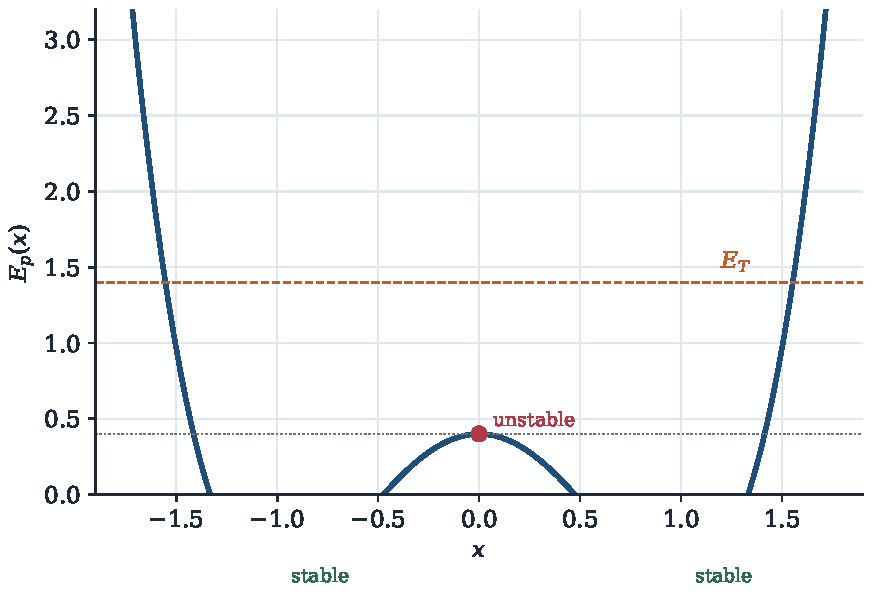
\includegraphics[width=0.74\textwidth]{figures/15_energy_well.pdf}
\caption{A one-dimensional potential energy curve $E_p(x)$ with total mechanical energy $E_m$. The particle oscillates between the classical turning points $x_1$ and $x_2$ where $E_m = E_p(x)$.}
\label{fig:energy_well}
\end{figure}

\section{Permitted Regions and Turning Points}

Since kinetic energy cannot be negative:
\[
E_c = \frac{1}{2}m v^2 = E_m - E_p(x) \ge 0 \implies \boxed{E_m \ge E_p(x).}
\]
\begin{itemize}[leftmargin=1.4em,itemsep=2pt]
  \item \textbf{Permitted region}: The set of positions where $E_p(x) \le E_m$.
  \item \textbf{Forbidden region}: Positions where $E_p(x) > E_m$ cannot be reached classically.
  \item \textbf{Turning points}: Positions $x_t$ where $E_p(x_t) = E_m$. At these points, $E_c = 0 \implies v = 0$. The particle stops and reverses direction.
  \item \textbf{Bound motion}: If the permitted region is bounded by two turning points $[x_1, x_2]$, the particle is trapped in a \textbf{potential well} and undergoes periodic oscillations.
\end{itemize}

\section{Equilibrium and Stability Criteria}

An equilibrium position $x_0$ satisfies $\left.\frac{\dd E_p}{\dd x}\right|_{x_0} = 0$. Its stability is determined by the second derivative:

\begin{center}
\renewcommand{\arraystretch}{1.3}
\begin{tabular}{@{}llll@{}}
\toprule
\textbf{Second Derivative} & \textbf{Geometry of $E_p(x)$} & \textbf{Stability} & \textbf{Restoring Force} \\
\midrule
$\left.\frac{\dd^2 E_p}{\dd x^2}\right|_{x_0} > 0$ & Local minimum (well) & \textbf{Stable} & $F \approx -k_{\text{eff}}(x-x_0)$ directed toward $x_0$ \\
$\left.\frac{\dd^2 E_p}{\dd x^2}\right|_{x_0} < 0$ & Local maximum (crest) & \textbf{Unstable} & $F \approx +k(x-x_0)$ pushes away from $x_0$ \\
$\left.\frac{\dd^2 E_p}{\dd x^2}\right|_{x_0} = 0$ & Flat inflection / plateau & \textbf{Neutral / Higher order} & Examine third and fourth derivatives \\
\bottomrule
\end{tabular}
\end{center}

\begin{figure}[htbp]
\centering
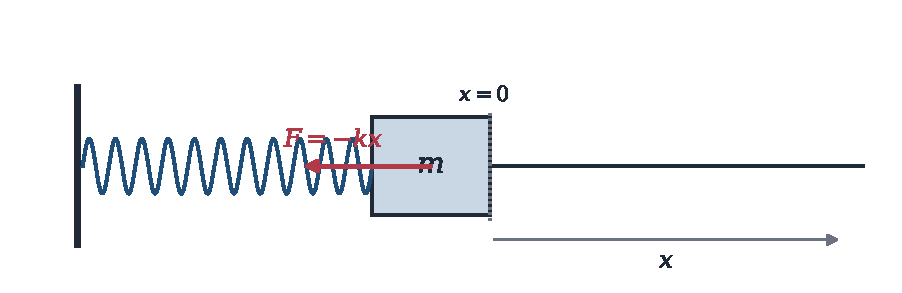
\includegraphics[width=0.68\textwidth]{figures/14_spring_mass.pdf}
\caption{The classic harmonic oscillator: a mass on a spring around its stable equilibrium position.}
\label{fig:spring_mass}
\end{figure}

\section{Small Oscillations around a Stable Minimum}

Let $x_0$ be a stable equilibrium point. Expand $E_p(x)$ in a Taylor series about $x_0$ for small displacements $\xi = x - x_0$:
\[
E_p(x) = E_p(x_0) + \underbrace{\left.\frac{\dd E_p}{\dd x}\right|_{x_0}}_{=0}\xi + \frac{1}{2}\underbrace{\left.\frac{\dd^2 E_p}{\dd x^2}\right|_{x_0}}_{\equiv k_{\text{eff}}}\xi^2 + \mathcal{O}(\xi^3).
\]
Dropping higher-order terms, the potential near the minimum is \textbf{parabolic}:
\[
\boxed{E_p(x) \approx E_p(x_0) + \frac{1}{2}k_{\text{eff}}\,\xi^2,} \quad \text{where } \boxed{k_{\text{eff}} = \left.\frac{\dd^2 E_p}{\dd x^2}\right|_{x_0} > 0.}
\]
The restoring force is linear in $\xi$:
\[
F(\xi) = -\frac{\dd E_p}{\dd\xi} \approx -k_{\text{eff}}\,\xi.
\]
Newton's second law $m\ddot{\xi} = -k_{\text{eff}}\xi$ becomes the equation of a \textbf{simple harmonic oscillator}:
\[
\boxed{\ddot{\xi} + \omega_0^2\,\xi = 0,} \quad \text{where } \boxed{\omega_0 = \sqrt{\frac{k_{\text{eff}}}{m}} = \sqrt{\left.\frac{1}{m}\frac{\dd^2 E_p}{\dd x^2}\right|_{x_0}}.}
\]
The period of small oscillations is:
\[
\boxed{T_0 = \frac{2\pi}{\omega_0} = 2\pi\sqrt{\frac{m}{k_{\text{eff}}}}.}
\]

\section{Worked Examples}

\begin{worked}[The Lennard-Jones (6-12) molecular potential]
The interaction between two noble gas atoms is modeled by the Lennard-Jones potential:
\[
U(r) = 4\epsilon\left[ \left(\frac{\sigma}{r}\right)^{12} - \left(\frac{\sigma}{r}\right)^6 \right],
\]
where $\epsilon$ is the depth of the potential well and $\sigma$ is the finite distance at which $U(\sigma) = 0$.
(a) Find the equilibrium bond length $r_0$ and the minimum potential energy $U(r_0)$.
(b) Calculate the effective spring constant $k_{\text{eff}}$ for small vibrations about $r_0$.
(c) Find the angular frequency $\omega_0$ of small vibrations for a reduced mass $\mu$.
\end{worked}

\begin{solution}{14.1}
(a) Set $\frac{\dd U}{\dd r} = 0$:
\[
\frac{\dd U}{\dd r} = 4\epsilon\left[ -12\frac{\sigma^{12}}{r^{13}} + 6\frac{\sigma^6}{r^7} \right] = \frac{24\epsilon}{r}\left[ \left(\frac{\sigma}{r}\right)^6 - 2\left(\frac{\sigma}{r}\right)^{12} \right].
\]
Setting this to zero:
\[
\left(\frac{\sigma}{r_0}\right)^6 = 2\left(\frac{\sigma}{r_0}\right)^{12} \implies \left(\frac{r_0}{\sigma}\right)^6 = 2 \implies \boxed{r_0 = 2^{1/6}\sigma \approx 1.1225\,\sigma.}
\]
The minimum potential energy is:
\[
U(r_0) = 4\epsilon\left[ \left(\frac{1}{2}\right)^2 - \frac{1}{2} \right] = 4\epsilon\left[ \frac{1}{4} - \frac{1}{2} \right] = \boxed{-\epsilon.}
\]
The dissociation energy required to separate the molecules to infinity is $\epsilon$.

(b) Compute the second derivative:
\[
\frac{\dd^2 U}{\dd r^2} = 4\epsilon\left[ 12\times 13\frac{\sigma^{12}}{r^{14}} - 6\times 7\frac{\sigma^6}{r^8} \right] = \frac{4\epsilon}{r^2}\left[ 156\left(\frac{\sigma}{r}\right)^{12} - 42\left(\frac{\sigma}{r}\right)^6 \right].
\]
Evaluating at $r = r_0$ where $(\sigma/r_0)^6 = 1/2$ and $(\sigma/r_0)^{12} = 1/4$:
\[
k_{\text{eff}} = \left.\frac{\dd^2 U}{\dd r^2}\right|_{r_0} = \frac{4\epsilon}{r_0^2}\left[ 156\left(\frac{1}{4}\right) - 42\left(\frac{1}{2}\right) \right] = \frac{4\epsilon}{r_0^2}\left[ 39 - 21 \right] = \frac{4\epsilon}{r_0^2}(18) = \boxed{\frac{72\epsilon}{r_0^2}.}
\]
Since $r_0^2 = 2^{1/3}\sigma^2$, this is $k_{\text{eff}} \approx \frac{57.14\epsilon}{\sigma^2} > 0$ (stable equilibrium!).

(c) The angular frequency of small vibrations is:
\[
\boxed{\omega_0 = \sqrt{\frac{k_{\text{eff}}}{\mu}} = \frac{1}{r_0}\sqrt{\frac{72\epsilon}{\mu}} = \frac{6}{r_0}\sqrt{\frac{2\epsilon}{\mu}}.}
\]
\end{solution}

\begin{worked}[Equilibrium and stability of a bead on an inverted parabola]
A bead of mass $m$ slides without friction on a rigid wire bent into the shape of a parabola $y = -\frac{1}{2}c x^2$ ($c > 0$) in a vertical plane, under gravity $\vec{g} = -g\jhat$.
Show that $x = 0$ is an unstable equilibrium, and find the characteristic time $\tau$ for the bead to fall away.
\end{worked}

\begin{solution}{14.2}
The potential energy of the bead in gravity is:
\[
E_p(x) = mgy = -mg\left(\frac{1}{2}c x^2\right) = -\frac{1}{2}mgc\,x^2.
\]
The first and second derivatives are:
\[
\frac{\dd E_p}{\dd x} = -mgc\,x,\qquad \frac{\dd^2 E_p}{\dd x^2} = -mgc.
\]
At $x = 0$, $\frac{\dd E_p}{\dd x} = 0$, so $x_0 = 0$ is an equilibrium point.
However:
\[
\left.\frac{\dd^2 E_p}{\dd x^2}\right|_{0} = -mgc < 0.
\]
Because the second derivative is strictly negative, the origin is a local maximum: it is an \textbf{unstable equilibrium}.
The equation of motion for small displacements ($\dot{x}^2 \ll 1 \implies \dd s \approx \dd x$) is:
\[
m\ddot{x} = -\frac{\dd E_p}{\dd x} = +mgc\,x \implies \ddot{x} - (gc)x = 0.
\]
The general solution is $x(t) = A e^{t/\tau} + B e^{-t/\tau}$ with characteristic time constant:
\[
\boxed{\tau = \frac{1}{\sqrt{gc}}.}
\]
Any tiny perturbation causes the displacement to grow exponentially with time constant $\tau$.
\end{solution}

\section{Exercises and Step-by-Step Solutions}

\begin{exercise}{\warm\ Classifying equilibria of a polynomial potential}
Consider a particle of mass $m=0.25\ \mathrm{kg}$ moving in the potential:
\[
E_p(x) = x^3 - 3x\quad (\text{with } x \text{ in metres, } E_p \text{ in joules}).
\]
(a) Find the positions of all equilibrium points.
(b) Determine the stability of each equilibrium point using the second derivative test.
(c) For the stable equilibrium point, calculate the effective spring constant $k_{\text{eff}}$ and the frequency $f_0$ of small oscillations.
\end{exercise}

\begin{tabletworkspace}[5.0cm]
\end{tabletworkspace}

\begin{solution}{14.1}
(a) Equilibria occur where $\frac{\dd E_p}{\dd x} = 0$:
\[
\frac{\dd E_p}{\dd x} = 3x^2 - 3 = 0 \implies x^2 = 1 \implies \mathbf{x_1 = -1.0\ \mathrm{m},\quad x_2 = +1.0\ \mathrm{m}.}
\]

(b) Second derivative:
\[
\frac{\dd^2 E_p}{\dd x^2} = 6x.
\]
\begin{itemize}[leftmargin=1.4em,itemsep=2pt]
  \item At $x_1 = -1.0\ \mathrm{m}$: $\left.\frac{\dd^2 E_p}{\dd x^2}\right|_{-1} = -6.0\ \mathrm{J\,m^{-2}} < 0 \implies$ \textbf{Unstable equilibrium} (local peak).
  \item At $x_2 = +1.0\ \mathrm{m}$: $\left.\frac{\dd^2 E_p}{\dd x^2}\right|_{+1} = +6.0\ \mathrm{J\,m^{-2}} > 0 \implies$ \textbf{Stable equilibrium} (local well).
\end{itemize}

(c) At the stable minimum $x_2 = 1.0\ \mathrm{m}$:
\[
k_{\text{eff}} = \left.\frac{\dd^2 E_p}{\dd x^2}\right|_{+1} = \mathbf{6.0\ \mathrm{N\,m^{-1}}.}
\]
The angular frequency is:
\[
\omega_0 = \sqrt{\frac{k_{\text{eff}}}{m}} = \sqrt{\frac{6.0}{0.25}} = \sqrt{24} \approx 4.90\ \mathrm{rad\,s^{-1}}.
\]
The oscillation frequency is:
\[
f_0 = \frac{\omega_0}{2\pi} = \frac{4.90}{2\pi} \approx \mathbf{0.78\ \mathrm{Hz}.}
\]
\end{solution}

\begin{exercise}{\warm\ Permitted regions and turning points from energy}
A particle of mass $m=1.0\ \mathrm{kg}$ moves along the $x$-axis in the potential $E_p(x) = \frac{1}{2}x^4 - 2x^2$ (in joules).
Its total mechanical energy is $E_m = -1.0\ \mathrm{J}$.
(a) Find the positions of the two potential minima and the potential barrier at $x = 0$.
(b) Find the turning points $x_t$ where $E_p(x) = E_m$.
(c) Identify the permitted intervals of motion for $E_m = -1.0\ \mathrm{J}$. Can a particle in the left well reach the right well?
\end{exercise}

\begin{tabletworkspace}[5.5cm]
\end{tabletworkspace}

\begin{solution}{14.2}
(a) Finding extrema:
\[
\frac{\dd E_p}{\dd x} = 2x^3 - 4x = 2x(x^2 - 2) = 0 \implies x = 0,\quad x = \pm\sqrt{2}.
\]
\begin{itemize}[leftmargin=1.4em,itemsep=2pt]
  \item At $x = 0$: $E_p(0) = 0\ \mathrm{J}$ (local maximum / potential barrier).
  \item At $x = \pm\sqrt{2}$: $E_p(\pm\sqrt{2}) = \frac{1}{2}(4) - 2(2) = 2 - 4 = -2.0\ \mathrm{J}$ (two symmetric minima).
\end{itemize}

(b) Turning points satisfy $E_p(x) = E_m = -1.0\ \mathrm{J}$:
\[
\frac{1}{2}x^4 - 2x^2 = -1.0 \iff x^4 - 4x^2 + 2 = 0.
\]
Let $u = x^2$:
\[
u^2 - 4u + 2 = 0 \implies u = \frac{4 \pm \sqrt{16 - 8}}{2} = 2 \pm \sqrt{2}.
\]
Since $2 - \sqrt{2} \approx 0.5858 > 0$ and $2 + \sqrt{2} \approx 3.4142$:
\[
x = \pm\sqrt{2 - \sqrt{2}} \approx \pm 0.765\ \mathrm{m},\qquad x = \pm\sqrt{2 + \sqrt{2}} \approx \pm 1.848\ \mathrm{m}.
\]

(c) The condition $E_p(x) \le E_m = -1.0\ \mathrm{J}$ requires:
\[
\text{Left well:}\quad x \in [-1.848\ \mathrm{m},\ -0.765\ \mathrm{m}], \qquad \text{Right well:}\quad x \in [+0.765\ \mathrm{m},\ +1.848\ \mathrm{m}].
\]
The interval $(-0.765\ \mathrm{m}, +0.765\ \mathrm{m})$ is classically \textbf{forbidden} because $E_p(x) > -1.0\ \mathrm{J}$ there (with a peak of $0\ \mathrm{J}$ at $x=0$).
Therefore, a classical particle starting in the left well is trapped forever and \textbf{cannot reach the right well} (in quantum mechanics, it could tunnel through).
\end{solution}

\begin{exercise}{\core\ The Morse potential for molecular bonds}
The potential energy between two atoms in a diatomic molecule (such as $\mathrm{HCl}$) is well approximated by the Morse potential:
\[
V(r) = D_e\left[ 1 - e^{-a(r - r_e)} \right]^2,
\]
where $D_e$ is the well depth, $r_e$ is the equilibrium separation, and $a$ is the width parameter.
(a) Verify that $r = r_e$ is the equilibrium separation and find $V(r_e)$.
(b) Compute the effective spring constant $k_{\text{eff}} = \left.\frac{\dd^2 V}{\dd r^2}\right|_{r_e}$.
(c) For $\mathrm{HCl}$, $D_e = 4.43\ \mathrm{eV} = 7.10\times 10^{-19}\ \mathrm{J}$, $a = 1.90\times 10^{10}\ \mathrm{m^{-1}}$, and reduced mass $\mu = 1.63\times 10^{-27}\ \mathrm{kg}$. Calculate $k_{\text{eff}}$ and the vibrational frequency $\nu = \omega_0 / 2\pi$.
\end{exercise}

\begin{tabletworkspace}[6.0cm]
\end{tabletworkspace}

\begin{solution}{14.3}
(a) First derivative:
\[
\frac{\dd V}{\dd r} = 2D_e\left[ 1 - e^{-a(r - r_e)} \right]\left[ a e^{-a(r - r_e)} \right] = 2a D_e e^{-a(r - r_e)}\left[ 1 - e^{-a(r - r_e)} \right].
\]
At $r = r_e$:
\[
\left.\frac{\dd V}{\dd r}\right|_{r_e} = 2a D_e(1)(1 - 1) = 0.
\]
Thus $r_e$ is indeed an equilibrium position.
The potential energy at equilibrium is $V(r_e) = D_e(1 - 1)^2 = \mathbf{0\ \mathrm{J}}$.

(b) Second derivative:
\begin{align*}
\frac{\dd^2 V}{\dd r^2} &= 2a D_e \frac{\dd}{\dd r}\left[ e^{-a(r - r_e)} - e^{-2a(r - r_e)} \right] \\
&= 2a D_e\left[ -a e^{-a(r - r_e)} + 2a e^{-2a(r - r_e)} \right] = 2a^2 D_e\left[ 2e^{-2a(r - r_e)} - e^{-a(r - r_e)} \right].
\end{align*}
Evaluating at $r = r_e$:
\[
k_{\text{eff}} = \left.\frac{\dd^2 V}{\dd r^2}\right|_{r_e} = 2a^2 D_e(2 - 1) = \boxed{2a^2 D_e.}
\]

(c) Numerical values:
\[
k_{\text{eff}} = 2(1.90\times 10^{10})^2\times(7.10\times 10^{-19}) = 2(3.61\times 10^{20})\times(7.10\times 10^{-19}) = \mathbf{512.6\ \mathrm{N\,m^{-1}}.}
\]
Vibrational angular frequency:
\[
\omega_0 = \sqrt{\frac{k_{\text{eff}}}{\mu}} = \sqrt{\frac{512.6}{1.63\times 10^{-27}}} = \sqrt{3.145\times 10^{29}} \approx 5.61\times 10^{14}\ \mathrm{rad\,s^{-1}}.
\]
Vibrational frequency:
\[
\nu = \frac{\omega_0}{2\pi} = \frac{5.61\times 10^{14}}{2\pi} \approx \mathbf{8.93\times 10^{13}\ \mathrm{Hz}} = 89.3\ \mathrm{THz}.
\]
(This corresponds to an infrared absorption wavelength $\lambda = c/\nu \approx 3.36\ \mu\mathrm{m}$, typical of molecular vibration).
\end{solution}

\begin{exercise}{\core\ Oscillations of a floating cylinder}
A uniform solid vertical cylinder of mass $m$, radius $R$, and length $H$ floats upright in a liquid of density $\rho$ ($\rho > m / (\pi R^2 H)$).
Let $z$ be the downward vertical displacement from its static equilibrium floating position.
(a) Determine the equilibrium submerged depth $h_0$.
(b) Show that the net restoring force for a small displacement $z$ is $F_z = -(\rho g \pi R^2)z$.
(c) Derive the effective potential energy $E_p(z)$ and show that the vertical bobbing frequency is $\omega_0 = \sqrt{\frac{g}{h_0}}$.
\end{exercise}

\begin{tabletworkspace}[5.5cm]
\end{tabletworkspace}

\begin{solution}{14.4}
(a) At static equilibrium, Archimedes' buoyant force balances gravity:
\[
F_B = \rho g V_{\text{sub}} = \rho g (\pi R^2 h_0) = mg \implies \boxed{h_0 = \frac{m}{\rho \pi R^2}.}
\]

(b) When the cylinder is displaced downward by $z$, the submerged depth increases to $h_0 + z$.
The buoyant force becomes $F_B(z) = \rho g \pi R^2(h_0 + z)$.
The net vertical force (with downward positive) is:
\[
F_{\text{net}} = mg - F_B(z) = mg - \rho g \pi R^2 h_0 - \rho g \pi R^2 z.
\]
Using $mg = \rho g \pi R^2 h_0$, the static terms cancel:
\[
\boxed{F_{\text{net}}(z) = -(\rho g \pi R^2)\,z.}
\]
The restoring force is purely linear (Hookean)!

(c) Potential energy:
\[
E_p(z) = -\int_0^z F_{\text{net}}(z')\dd z' = \frac{1}{2}(\rho g \pi R^2)z^2.
\]
Since $\frac{\dd^2 E_p}{\dd z^2} = \rho g \pi R^2 = k_{\text{eff}} > 0$, the equilibrium is unconditionally stable.
Newton's second law gives:
\[
m\ddot{z} + (\rho g \pi R^2)z = 0 \implies \ddot{z} + \omega_0^2 z = 0,
\]
with angular frequency:
\[
\omega_0 = \sqrt{\frac{\rho g \pi R^2}{m}}.
\]
Substituting $m = \rho \pi R^2 h_0$:
\[
\boxed{\omega_0 = \sqrt{\frac{g}{h_0}}.}
\]
Remarkably, the bobbing frequency of any floating cylinder depends solely on its submerged depth $h_0$, identical to a simple pendulum of length $L = h_0$!
\end{solution}

\begin{exercise}{\mastery\ Mass between two pre-tensioned transverse springs}
A particle of mass $m$ can slide along a smooth horizontal $x$-axis. It is held between two identical horizontal springs perpendicular to the $x$-axis, each of spring constant $k$ and natural length $\ell_0$, attached to fixed posts at $(0, +d)$ and $(0, -d)$ with $d > \ell_0$ (pre-tensioned).
(a) Express the total potential energy $E_p(x)$ of the two springs as a function of the transverse displacement $x$.
(b) Expand $E_p(x)$ in powers of $x$ up to order $x^4$.
(c) Find the effective spring constant $k_{\text{eff}}$ at $x = 0$ and the frequency $\omega_0$ of small oscillations.
(d) What happens if the posts are moved to $d = \ell_0$ (unstretched at $x=0$) or $d < \ell_0$ (compressed)?
\end{exercise}

\begin{tabletworkspace}[6.5cm]
\end{tabletworkspace}

\begin{solution}{14.5}
(a) The distance from the mass at $(x, 0)$ to either post at $(0, \pm d)$ is $\ell(x) = \sqrt{x^2 + d^2}$.
The extension of each spring is $\Delta\ell = \ell(x) - \ell_0 = \sqrt{x^2 + d^2} - \ell_0$.
The total potential energy of both identical springs is:
\[
\boxed{E_p(x) = 2\times\frac{1}{2}k\left( \sqrt{x^2 + d^2} - \ell_0 \right)^2 = k\left( \sqrt{x^2 + d^2} - \ell_0 \right)^2.}
\]

(b) For small displacements $x \ll d$:
\[
\sqrt{x^2 + d^2} = d\sqrt{1 + \frac{x^2}{d^2}} \approx d\left( 1 + \frac{1}{2}\frac{x^2}{d^2} - \frac{1}{8}\frac{x^4}{d^4} \right).
\]
The extension is:
\[
\sqrt{x^2 + d^2} - \ell_0 \approx (d - \ell_0) + \frac{x^2}{2d} - \frac{x^4}{8d^3}.
\]
Squaring this:
\begin{align*}
E_p(x) &\approx k\left[ (d - \ell_0)^2 + 2(d - \ell_0)\frac{x^2}{2d} + \frac{x^4}{4d^2} - 2(d - \ell_0)\frac{x^4}{8d^3} \right] \\
&= k(d - \ell_0)^2 + k\left(1 - \frac{\ell_0}{d}\right)x^2 + \frac{k\ell_0}{4d^3}x^4.
\end{align*}

(c) The linear restoring term corresponds to the coefficient of $\frac{1}{2}x^2$:
\[
\frac{1}{2}k_{\text{eff}} = k\left(1 - \frac{\ell_0}{d}\right) \implies \boxed{k_{\text{eff}} = 2k\left(1 - \frac{\ell_0}{d}\right).}
\]
Since $d > \ell_0$, $k_{\text{eff}} > 0$: the equilibrium at $x = 0$ is \textbf{stable}.
The angular frequency of small transverse oscillations is:
\[
\boxed{\omega_0 = \sqrt{\frac{2k}{m}\left(1 - \frac{\ell_0}{d}\right)}.}
\]

(d) Physical discussion of regimes:
\begin{itemize}[leftmargin=1.4em,itemsep=2pt]
  \item If $d = \ell_0$ (unstretched at $x=0$): $k_{\text{eff}} = 0$. The harmonic term vanishes! The potential becomes quartic: $E_p(x) \approx \frac{k}{4d^2}x^4$. The restoring force is non-linear ($F \propto -x^3$), and the oscillation frequency depends on amplitude!
  \item If $d < \ell_0$ (springs compressed at $x=0$): $k_{\text{eff}} < 0$. The origin $x = 0$ becomes \textbf{unstable}! The compressed springs buckle to the left or right, creating two new symmetric stable equilibrium points at $x_e = \pm\sqrt{\ell_0^2 - d^2}$.
\end{itemize}
\end{solution}

\chapter{Harmonic, Damped, and Driven Oscillations}
\label{ch:oscillations}
\begin{chapterintro}
\textbf{You will learn to:} solve the differential equations of free, damped, and forced harmonic oscillators; analyze underdamped, critically damped, and overdamped regimes; determine the quality factor $Q$ and logarithmic decrement; calculate resonance frequency, amplitude, and phase lag; and study energy dissipation and resonance bandwidth.
\end{chapterintro}

\section{The Simple Harmonic Oscillator}

The ideal undamped harmonic oscillator obeys the linear differential equation:
\[
\boxed{\ddot{x} + \omega_0^2\,x = 0,}
\]
where $\omega_0 = \sqrt{k/m}$ is the \textbf{natural angular frequency}.
The general solution can be written in equivalent forms:
\[
\boxed{x(t) = A\cos(\omega_0 t + \phi) = C_1\cos(\omega_0 t) + C_2\sin(\omega_0 t) = \operatorname{Re}\left( \tilde{X} e^{\mathrm{i}\omega_0 t} \right),}
\]
where $A$ is the amplitude and $\phi$ is the initial phase determined by initial conditions:
\[
A = \sqrt{x_0^2 + \left(\frac{v_0}{\omega_0}\right)^2}, \qquad \tan\phi = -\frac{v_0}{\omega_0 x_0}.
\]
The period and frequency are:
\[
T_0 = \frac{2\pi}{\omega_0} = 2\pi\sqrt{\frac{m}{k}}, \qquad f_0 = \frac{1}{T_0} = \frac{\omega_0}{2\pi}.
\]

\begin{figure}[htbp]
\centering
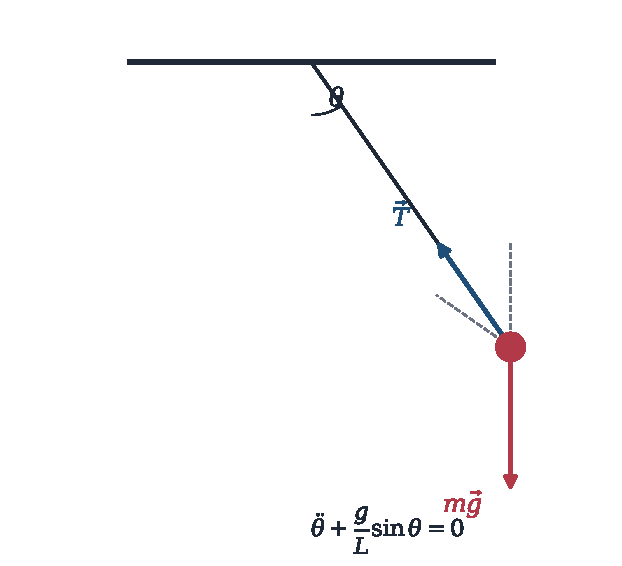
\includegraphics[width=0.48\textwidth]{figures/20_pendulum.pdf}
\caption{The simple pendulum of length $L$ oscillating at angle $\theta$ from the vertical. For small angles $\theta \ll 1$, it executes simple harmonic motion with natural frequency $\omega_0 = \sqrt{g/L}$.}
\label{fig:pendulum}
\end{figure}
The total mechanical energy is conserved:
\[
\boxed{E_m = \frac{1}{2}m v^2 + \frac{1}{2}k x^2 = \frac{1}{2}k A^2 = \frac{1}{2}m\omega_0^2 A^2 = \text{constant}.}
\]
Over one complete cycle, kinetic and potential energies share the total energy equally on average:
\[
\langle E_c \rangle = \langle E_p \rangle = \frac{1}{2}E_m.
\]

\begin{figure}[htbp]
\centering
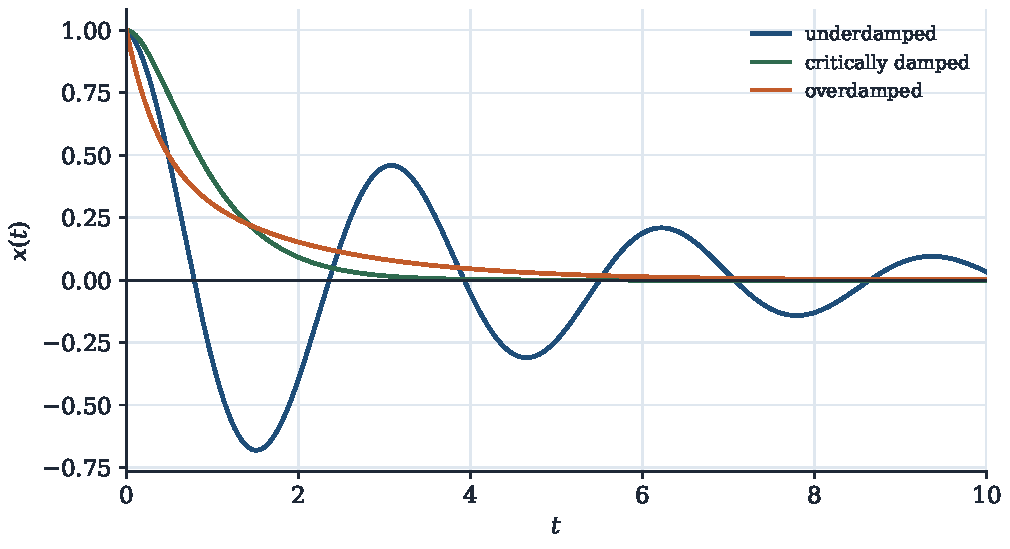
\includegraphics[width=0.74\textwidth]{figures/16_damped_oscillations.pdf}
\caption{Free damped oscillations in the underdamped regime ($\lambda < \omega_0$). The displacement decays within an exponential envelope $\pm A_0 e^{-\lambda t}$.}
\label{fig:damped_oscillations}
\end{figure}

\section{Damped Harmonic Oscillations}

When a viscous damping force $\vec{f} = -b\vec{v} = -b\dot{x}\ihat$ ($b > 0$) opposes motion, Newton's second law gives:
\[
m\ddot{x} + b\dot{x} + kx = 0 \implies \boxed{\ddot{x} + 2\lambda\dot{x} + \omega_0^2\,x = 0,}
\]
where $\lambda = \frac{b}{2m}$ is the \textbf{damping parameter}.
The characteristic equation is $r^2 + 2\lambda r + \omega_0^2 = 0$, with roots $r_{1, 2} = -\lambda \pm \sqrt{\lambda^2 - \omega_0^2}$.

Three distinct physical regimes arise depending on the discriminant $\Delta = \lambda^2 - \omega_0^2$:

\begin{center}
\renewcommand{\arraystretch}{1.3}
\begin{tabular}{@{}llll@{}}
\toprule
\textbf{Regime} & \textbf{Condition} & \textbf{General Solution $x(t)$} & \textbf{Physical Behavior} \\
\midrule
\textbf{Underdamped} & $\lambda < \omega_0$ & $A_0 e^{-\lambda t}\cos(\omega_d t + \phi)$ & Oscillations with decaying amplitude; $\omega_d = \sqrt{\omega_0^2 - \lambda^2}$ \\
\textbf{Critically Damped} & $\lambda = \omega_0$ & $(C_1 + C_2 t)e^{-\lambda t}$ & Fastest return to equilibrium without oscillating \\
\textbf{Overdamped} & $\lambda > \omega_0$ & $C_1 e^{r_1 t} + C_2 e^{r_2 t}$ & Sluggish non-oscillatory exponential return \\
\bottomrule
\end{tabular}
\end{center}

\begin{keyidea}[Key Parameters of Damped Systems]
\begin{itemize}[leftmargin=1.4em,itemsep=2pt]
  \item \textbf{Pseudo-period}: $T_d = \frac{2\pi}{\omega_d} = \frac{2\pi}{\sqrt{\omega_0^2 - \lambda^2}} > T_0$.
  \item \textbf{Logarithmic decrement}: The natural logarithm of the ratio of two successive peak displacements separated by one period $T_d$:
        \[
        \boxed{\delta = \ln\left(\frac{x(t)}{x(t + T_d)}\right) = \lambda T_d = \frac{2\pi\lambda}{\omega_d}.}
        \]
  \item \textbf{Quality factor $Q$}: Dimensionless figure of merit measuring sharpness of resonance and low dissipation:
        \[
        \boxed{Q = \frac{\omega_0}{2\lambda} = \frac{m\omega_0}{b} \approx \frac{\pi}{\delta}.}
        \]
        In one cycle, the fractional energy lost is $\frac{\Delta E_m}{E_m} \approx \frac{2\pi}{Q}$.
\end{itemize}
\end{keyidea}

\section{Driven (Forced) Oscillations and Resonance}

Apply an external sinusoidal driving force $F(t) = F_0\cos(\omega t)$:
\[
\boxed{\ddot{x} + 2\lambda\dot{x} + \omega_0^2\,x = \frac{F_0}{m}\cos(\omega t).}
\]
After transients die out, the \textbf{steady-state response} is sinusoidal at the driving frequency $\omega$:
\[
\boxed{x_p(t) = X(\omega)\cos(\omega t - \phi),}
\]
where the steady-state amplitude $X(\omega)$ and phase lag $\phi(\omega)$ are:
\[
\boxed{X(\omega) = \frac{F_0/m}{\sqrt{(\omega_0^2 - \omega^2)^2 + 4\lambda^2\omega^2}},} \qquad \boxed{\tan\phi(\omega) = \frac{2\lambda\omega}{\omega_0^2 - \omega^2}.}
\]

\begin{keyidea}[Resonance Phenomena]
\begin{itemize}[leftmargin=1.4em,itemsep=2pt]
  \item \textbf{Amplitude Resonance}: The amplitude $X(\omega)$ reaches its maximum at the \textbf{resonance frequency}:
        \[
        \boxed{\omega_{\text{res}} = \sqrt{\omega_0^2 - 2\lambda^2} = \omega_0\sqrt{1 - \frac{1}{2Q^2}}.}
        \]
        (Resonance occurs only if $\lambda < \omega_0/\sqrt{2}$, i.e., $Q > 1/\sqrt{2}$).
  \item \textbf{Peak Amplitude}: At $\omega = \omega_{\text{res}}$:
        \[
        X_{\max} = \frac{F_0/m}{2\lambda\sqrt{\omega_0^2 - \lambda^2}} \approx Q\left(\frac{F_0}{k}\right) \quad (\text{for } Q \gg 1).
        \]
        The static deflection $x_{\text{static}} = F_0/k$ is magnified by a factor of $Q$!
  \item \textbf{Velocity Resonance}: The velocity amplitude is maximized exactly at $\omega = \omega_0$, where the response is in \textbf{quadrature} ($\phi = \pi/2$), meaning the driving force is always in phase with velocity ($P(t) \ge 0$).
  \item \textbf{Resonance Bandwidth}: The width between half-power points ($\Delta\omega = \omega_2 - \omega_1$) satisfies:
        \[
        \boxed{\Delta\omega = 2\lambda = \frac{\omega_0}{Q}.}
        \]
\end{itemize}
\end{keyidea}

\section{Worked Examples}

\begin{worked}[Determining damping and $Q$ from an oscilloscope trace]
An underdamped mechanical oscillator of mass $m=0.100\ \mathrm{kg}$ has a natural frequency $f_0 = 5.00\ \mathrm{Hz}$. Its recorded amplitude drops from $x_0 = 4.00\ \mathrm{cm}$ to $x_{10} = 1.00\ \mathrm{cm}$ after $N = 10$ full oscillations.
Find the logarithmic decrement $\delta$, the damping constant $\lambda$, the quality factor $Q$, and the damping coefficient $b$.
\end{worked}

\begin{solution}{15.1}
The amplitude after $N$ cycles decays according to $x_N = x_0 e^{-N\lambda T_d}$:
\[
\frac{x_0}{x_N} = e^{N\lambda T_d} = e^{N\delta} \implies N\delta = \ln\left(\frac{x_0}{x_N}\right).
\]
For $N = 10$ and $x_0/x_{10} = 4.00/1.00 = 4.00$:
\[
10\delta = \ln(4.00) = 1.3863 \implies \boxed{\delta = \frac{1.3863}{10} \approx \mathbf{0.1386.}}
\]
Since $\delta \ll 1$, damping is weak, so $\omega_d \approx \omega_0$:
\[
T_d \approx T_0 = \frac{1}{f_0} = \frac{1}{5.00} = 0.200\ \mathrm{s}.
\]
The damping parameter is:
\[
\lambda = \frac{\delta}{T_d} = \frac{0.1386}{0.200} = \mathbf{0.693\ \mathrm{s^{-1}}.}
\]
The quality factor is:
\[
Q = \frac{\pi}{\delta} = \frac{\pi}{0.1386} \approx \mathbf{22.7.}
\]
The viscous damping coefficient is:
\[
b = 2m\lambda = 2(0.100\ \mathrm{kg})(0.693\ \mathrm{s^{-1}}) = \mathbf{0.139\ \mathrm{kg\,s^{-1}}.}
\]
\end{solution}

\begin{worked}[Driven oscillator at resonance]
A spring-mass system with $m = 0.500\ \mathrm{kg}$, $k = 200\ \mathrm{N\,m^{-1}}$, and $b = 0.800\ \mathrm{kg\,s^{-1}}$ is driven by an external force $F(t) = F_0\cos(\omega t)$ with $F_0 = 4.00\ \mathrm{N}$.
(a) Find the natural angular frequency $\omega_0$, damping factor $\lambda$, and quality factor $Q$.
(b) Find the resonance frequency $\omega_{\text{res}}$ and the amplitude at resonance $X_{\max}$.
(c) Compute the average power supplied by the driver at velocity resonance ($\omega = \omega_0$).
\end{worked}

\begin{solution}{15.2}
(a) Fundamental parameters:
\[
\omega_0 = \sqrt{\frac{k}{m}} = \sqrt{\frac{200}{0.500}} = \mathbf{20.0\ \mathrm{rad\,s^{-1}}.}
\]
\[
\lambda = \frac{b}{2m} = \frac{0.800}{2(0.500)} = \mathbf{0.800\ \mathrm{s^{-1}}.}
\]
\[
Q = \frac{\omega_0}{2\lambda} = \frac{20.0}{2(0.800)} = \mathbf{12.5.}
\]

(b) Resonance frequency:
\[
\omega_{\text{res}} = \sqrt{\omega_0^2 - 2\lambda^2} = \sqrt{20.0^2 - 2(0.800)^2} = \sqrt{400 - 1.28} = \sqrt{398.72} \approx \mathbf{19.97\ \mathrm{rad\,s^{-1}}.}
\]
The amplitude at resonance is:
\[
X_{\max} = \frac{F_0/m}{2\lambda\sqrt{\omega_0^2 - \lambda^2}} = \frac{4.00/0.500}{2(0.800)\sqrt{400 - 0.64}} = \frac{8.00}{1.60\times 19.98} = \frac{8.00}{31.97} \approx \mathbf{0.250\ \mathrm{m}} = 25.0\ \mathrm{cm}.
\]
Notice that static deflection is $x_{\text{st}} = F_0/k = 4.00/200 = 0.020\ \mathrm{m} = 2.0\ \mathrm{cm}$. The resonance magnifies the motion by a factor of $X_{\max}/x_{\text{st}} = 25.0/2.0 = 12.5 = Q$!

(c) At $\omega = \omega_0 = 20.0\ \mathrm{rad\,s^{-1}}$, the force and velocity are in phase ($\phi = \pi/2$). The velocity amplitude is $V_0 = \omega_0 X(\omega_0) = \frac{F_0}{b}$:
\[
V_0 = \frac{4.00}{0.800} = 5.00\ \mathrm{m\,s^{-1}}.
\]
The average power supplied by the driver (which equals the power dissipated by friction) is:
\[
\langle P \rangle = \frac{1}{2}F_0 V_0 = \frac{1}{2}(4.00\ \mathrm{N})(5.00\ \mathrm{m\,s^{-1}}) = \mathbf{10.0\ \mathrm{W}.}
\]
\end{solution}

\section{Exercises and Step-by-Step Solutions}

\begin{exercise}{\warm\ General solution from initial conditions}
A horizontal spring-mass oscillator has mass $m=0.200\ \mathrm{kg}$ and spring stiffness $k=80.0\ \mathrm{N\,m^{-1}}$. At $t=0$, the mass is displaced to $x_0 = +5.00\ \mathrm{cm} = 0.0500\ \mathrm{m}$ and given an initial velocity $v_0 = -0.600\ \mathrm{m\,s^{-1}}$ directed toward the origin.
(a) Find the natural angular frequency $\omega_0$ and the period $T_0$.
(b) Write the position $x(t) = A\cos(\omega_0 t + \phi)$, finding $A$ and $\phi$.
(c) Calculate the total mechanical energy $E_m$.
\end{exercise}

\begin{tabletworkspace}[5.0cm]
\end{tabletworkspace}

\begin{solution}{15.1}
(a) Angular frequency:
\[
\omega_0 = \sqrt{\frac{k}{m}} = \sqrt{\frac{80.0}{0.200}} = \sqrt{400} = \mathbf{20.0\ \mathrm{rad\,s^{-1}}.}
\]
Period:
\[
T_0 = \frac{2\pi}{\omega_0} = \frac{2\pi}{20.0} = \frac{\pi}{10} \approx \mathbf{0.314\ \mathrm{s}.}
\]

(b) Amplitude:
\[
A = \sqrt{x_0^2 + \left(\frac{v_0}{\omega_0}\right)^2} = \sqrt{(0.0500)^2 + \left(\frac{-0.600}{20.0}\right)^2} = \sqrt{0.00250 + (-0.0300)^2} = \sqrt{0.00250 + 0.00090} = \sqrt{0.00340} \approx \mathbf{0.0583\ \mathrm{m}} = 5.83\ \mathrm{cm}.
\]
Phase angle $\phi$:
\[
\tan\phi = -\frac{v_0}{\omega_0 x_0} = -\frac{-0.600}{20.0\times 0.0500} = +\frac{0.600}{1.000} = +0.600.
\]
Since $x_0 > 0$ and $\cos\phi = x_0/A > 0$, $\phi$ is in the first quadrant:
\[
\phi = \arctan(0.600) \approx 0.540\ \mathrm{rad} \approx 31.0^\circ.
\]
The full trajectory is:
\[
\boxed{x(t) = 0.0583\cos(20.0 t + 0.540)\ \mathrm{m}.}
\]

(c) Mechanical energy:
\[
E_m = \frac{1}{2}k A^2 = \frac{1}{2}(80.0)(0.0583)^2 = 40.0\times 0.00340 = \mathbf{0.136\ \mathrm{J}.}
\]
Check with initial values: $E_m = \frac{1}{2}k x_0^2 + \frac{1}{2}m v_0^2 = \frac{1}{2}(80.0)(0.05)^2 + \frac{1}{2}(0.20)(-0.6)^2 = 0.100 + 0.036 = 0.136\ \mathrm{J}$ (exact agreement!).
\end{solution}

\begin{exercise}{\warm\ The Virial Theorem for harmonic oscillations}
For an undamped harmonic oscillator $x(t) = A\cos(\omega_0 t + \phi)$:
(a) Write the instantaneous kinetic energy $E_c(t)$ and potential energy $E_p(t)$.
(b) Calculate the time-average of both energies over one complete period $T_0$:
\[
\langle E_c \rangle = \frac{1}{T_0}\int_0^{T_0} E_c(t)\dd t, \qquad \langle E_p \rangle = \frac{1}{T_0}\int_0^{T_0} E_p(t)\dd t.
\]
(c) Verify that $\langle E_c \rangle = \langle E_p \rangle = \frac{1}{2}E_m$.
\end{exercise}

\begin{tabletworkspace}[5.0cm]
\end{tabletworkspace}

\begin{solution}{15.2}
(a) The position and velocity are:
\[
x(t) = A\cos(\omega_0 t + \phi), \qquad v(t) = \dot{x}(t) = -\omega_0 A\sin(\omega_0 t + \phi).
\]
Instantaneous energies:
\begin{align*}
E_p(t) &= \frac{1}{2}k x^2(t) = \frac{1}{2}k A^2\cos^2(\omega_0 t + \phi), \\
E_c(t) &= \frac{1}{2}m v^2(t) = \frac{1}{2}m\omega_0^2 A^2\sin^2(\omega_0 t + \phi) = \frac{1}{2}k A^2\sin^2(\omega_0 t + \phi).
\end{align*}

(b) Using the standard trigonometric integral averages:
\[
\frac{1}{T_0}\int_0^{T_0} \cos^2(\omega_0 t + \phi)\dd t = \frac{1}{2}, \qquad \frac{1}{T_0}\int_0^{T_0} \sin^2(\omega_0 t + \phi)\dd t = \frac{1}{2}.
\]
Therefore:
\begin{align*}
\langle E_p \rangle &= \frac{1}{2}k A^2\left(\frac{1}{2}\right) = \mathbf{\frac{1}{4}k A^2,} \\
\langle E_c \rangle &= \frac{1}{2}k A^2\left(\frac{1}{2}\right) = \mathbf{\frac{1}{4}k A^2.}
\end{align*}

(c) The total energy is $E_m = \frac{1}{2}k A^2$.
Comparing:
\[
\boxed{\langle E_c \rangle = \langle E_p \rangle = \frac{1}{2}E_m.}
\]
This equipartition of energy on average between kinetic and potential forms is a fundamental instance of the Virial Theorem for quadratic potentials ($V \propto r^2 \implies 2\langle E_c \rangle = 2\langle E_p \rangle$).
\end{solution}

\begin{exercise}{\core\ Critical damping for an automobile suspension}
A car wheel and suspension can be modeled as a quarter-car of mass $m=350\ \mathrm{kg}$ supported by a spring of stiffness $k=35.0\ \mathrm{kN\,m^{-1}} = 35000\ \mathrm{N\,m^{-1}}$ and a shock absorber (dashpot) of damping coefficient $b$.
(a) Find the natural angular frequency $\omega_0$ and the undamped oscillation frequency $f_0$.
(b) Calculate the critical damping coefficient $b_{\text{crit}}$ required for the suspension to return to equilibrium as quickly as possible without bouncing.
(c) If the shock absorber wears out and its damping drops to $b = 0.25\,b_{\text{crit}}$, find the pseudo-period $T_d$ and the fraction of amplitude remaining after one bounce.
\end{exercise}

\begin{tabletworkspace}[5.5cm]
\end{tabletworkspace}

\begin{solution}{15.3}
(a) Natural angular frequency:
\[
\omega_0 = \sqrt{\frac{k}{m}} = \sqrt{\frac{35000}{350}} = \sqrt{100} = \mathbf{10.0\ \mathrm{rad\,s^{-1}}.}
\]
Frequency:
\[
f_0 = \frac{\omega_0}{2\pi} = \frac{10.0}{2\pi} \approx \mathbf{1.59\ \mathrm{Hz}.}
\]

(b) Critical damping occurs when $\lambda = \omega_0$:
\[
\frac{b_{\text{crit}}}{2m} = \omega_0 \implies \boxed{b_{\text{crit}} = 2m\omega_0 = 2\sqrt{km}.}
\]
Computing:
\[
b_{\text{crit}} = 2(350)(10.0) = \mathbf{7000\ \mathrm{N\,s\,m^{-1}}} = 7.00\times 10^3\ \mathrm{kg\,s^{-1}}.
\]

(c) Worn shock absorber: $b = 0.25\,b_{\text{crit}} \implies \lambda = 0.25\,\omega_0 = 2.50\ \mathrm{s^{-1}}$.
The pseudo-frequency is:
\[
\omega_d = \sqrt{\omega_0^2 - \lambda^2} = \sqrt{10.0^2 - 2.5^2} = \sqrt{100 - 6.25} = \sqrt{93.75} \approx 9.68\ \mathrm{rad\,s^{-1}}.
\]
The pseudo-period is:
\[
T_d = \frac{2\pi}{\omega_d} = \frac{2\pi}{9.68} \approx \mathbf{0.649\ \mathrm{s}.}
\]
The decay per period is given by the factor $e^{-\lambda T_d}$:
\[
\lambda T_d = (2.50)(0.649) \approx 1.623 \implies \frac{A(t + T_d)}{A(t)} = e^{-1.623} \approx \mathbf{0.197} \approx 19.7\%.
\]
The car will noticeably bounce after hitting a pothole, retaining nearly $20\%$ of its displacement on the rebound!
\end{solution}

\begin{exercise}{\core\ Oscillations in a U-tube manometer}
A uniform glass U-tube of internal cross-sectional area $S$ contains a column of liquid of density $\rho$ and total column length $L$. The liquid is displaced by a distance $z_0$ in one arm and released.
(a) Neglecting viscosity, show that the column executes simple harmonic motion with equation:
\[
\ddot{z} + \frac{2g}{L}z = 0.
\]
(b) Find the period of oscillation $T$. Compare it with a simple pendulum.
(c) Liquid viscosity introduces a Poiseuille laminar drag force $F_d = -8\pi\eta L\dot{z}$, where $\eta$ is the dynamic viscosity. Write the damped differential equation and determine the condition on $\eta$ for the motion to remain underdamped.
\end{exercise}

\begin{tabletworkspace}[6.0cm]
\end{tabletworkspace}

\begin{solution}{15.4}
(a) The total mass of the liquid column is $m = \rho S L$.
When the liquid level rises by $z$ in the right arm, it drops by $z$ in the left arm.
The height difference between the two columns is $2z$.
The unbalanced weight of this excess column provides the restoring force:
\[
F_{\text{rest}} = -(\text{mass of excess column})g = -(\rho S\cdot 2z)g = -2\rho g S z.
\]
Applying Newton's second law $m\ddot{z} = F_{\text{rest}}$:
\[
(\rho S L)\ddot{z} = -2\rho g S z \implies \rho S L\ddot{z} + 2\rho g S z = 0.
\]
Dividing by $\rho S L$:
\[
\boxed{\ddot{z} + \frac{2g}{L}z = 0.}
\]

(b) The natural angular frequency is $\omega_0 = \sqrt{\frac{2g}{L}}$.
The period of oscillation is:
\[
\boxed{T = 2\pi\sqrt{\frac{L}{2g}}.}
\]
This is identical to the period of a simple pendulum of length $L_{\text{eff}} = \frac{L}{2}$!

(c) Adding the laminar viscous friction force $F_d = -b\dot{z}$ with $b = 8\pi\eta L$:
\[
m\ddot{z} + b\dot{z} + (2\rho g S)z = 0 \implies \ddot{z} + \frac{8\pi\eta}{\rho S}\dot{z} + \frac{2g}{L}z = 0.
\]
The damping parameter is $\lambda = \frac{b}{2m} = \frac{8\pi\eta L}{2\rho S L} = \frac{4\pi\eta}{\rho S}$.
For the motion to remain \textbf{underdamped} ($\lambda < \omega_0$):
\[
\frac{4\pi\eta}{\rho S} < \sqrt{\frac{2g}{L}} \implies \boxed{\eta < \frac{\rho S}{4\pi}\sqrt{\frac{2g}{L}}.}
\]
\end{solution}

\begin{exercise}{\mastery\ Two coupled oscillators and normal modes}
Two identical carts, each of mass $m$, can move along a frictionless horizontal track. Each cart is connected to a rigid wall by a spring of stiffness $k$, and the two carts are coupled to each other by a central spring of stiffness $k_c$.
(a) Write Newton's second law for displacements $x_1(t)$ and $x_2(t)$ from equilibrium.
(b) Define the \textbf{normal coordinates} $u(t) = x_1 + x_2$ (symmetric mode) and $v(t) = x_1 - x_2$ (antisymmetric mode). Show that they decouple into two independent harmonic oscillators.
(c) Find the two normal frequencies $\omega_1$ and $\omega_2$, and describe the physical motion in each mode.
\end{exercise}

\begin{tabletworkspace}[6.5cm]
\end{tabletworkspace}

\begin{solution}{15.5}
(a) The forces on each cart are:
\begin{align*}
m\ddot{x}_1 &= -kx_1 + k_c(x_2 - x_1) = -(k + k_c)x_1 + k_c x_2, \\
m\ddot{x}_2 &= -kx_2 - k_c(x_2 - x_1) = k_c x_1 - (k + k_c)x_2.
\end{align*}

(b) Adding the two equations:
\[
m(\ddot{x}_1 + \ddot{x}_2) = -k(x_1 + x_2) \implies m\ddot{u} + k u = 0 \implies \boxed{\ddot{u} + \omega_1^2 u = 0,}
\]
where $\omega_1 = \sqrt{\frac{k}{m}}$.

Subtracting the two equations:
\[
m(\ddot{x}_1 - \ddot{x}_2) = -(k + 2k_c)(x_1 - x_2) \implies m\ddot{v} + (k + 2k_c)v = 0 \implies \boxed{\ddot{v} + \omega_2^2 v = 0,}
\]
where $\omega_2 = \sqrt{\frac{k + 2k_c}{m}}$.
The normal coordinates $u(t)$ and $v(t)$ are completely decoupled!

(c) Physical description of the normal modes:
\begin{itemize}[leftmargin=1.4em,itemsep=2pt]
  \item \textbf{Mode 1 (Symmetric / In-phase)}: $v = 0 \implies x_1(t) = x_2(t)$.
  Frequency: $\boxed{\omega_1 = \sqrt{\frac{k}{m}}}$.
  Both carts move synchronously in the same direction with identical amplitude. The coupling spring maintains constant length ($x_2 - x_1 = 0$) and exerts no force; the carts oscillate as if the central spring did not exist!
  \item \textbf{Mode 2 (Antisymmetric / Out-of-phase)}: $u = 0 \implies x_1(t) = -x_2(t)$.
  Frequency: $\boxed{\omega_2 = \sqrt{\frac{k + 2k_c}{m}}}$.
  The carts move in opposite directions, alternately compressing and expanding the central spring. The restoring force is stronger, so $\omega_2 > \omega_1$.
\end{itemize}
Any general motion is a linear superposition $x_1(t) = \frac{1}{2}(u(t) + v(t))$ and $x_2(t) = \frac{1}{2}(u(t) - v(t))$, giving rise to the phenomenon of \textbf{beats} when $k_c \ll k$.
\end{solution}


\part{Mastery}

\chapter{Systems of Particles, Collisions, and Synoptic Mastery}
\label{ch:systems_collisions}
\begin{chapterintro}
\textbf{You will learn to:} locate the center of mass of discrete systems; apply the momentum conservation theorem to isolated systems; solve 1D and 2D elastic and inelastic collisions using the coefficient of restitution; transform between laboratory and center-of-mass frames using Koenig's theorems and reduced mass $\mu$; derive the Tsiolkovsky rocket equation; and tackle comprehensive multi-stage exam synthesis problems.
\end{chapterintro}

\section{Center of Mass and Total Momentum}

For a system of $N$ material points with masses $m_i$ and positions $\vec{r}_i$:
\begin{itemize}[leftmargin=1.4em,itemsep=3pt]
  \item The \textbf{total mass} is $M = \sum_{i=1}^N m_i$.
  \item The \textbf{center of mass} (CM) position $G$ is defined by:
        \[
        \boxed{\vec{r}_G = \frac{1}{M}\sum_{i=1}^N m_i\vec{r}_i.}
        \]
  \item The \textbf{total linear momentum} is:
        \[
        \boxed{\vec{P}_{\text{tot}} = \sum_{i=1}^N m_i\vec{v}_i = M\vec{v}_G.}
        \]
\end{itemize}

Differentiating with respect to time and separating forces into external forces $\vec{F}_{i,\text{ext}}$ and internal mutual forces $\vec{F}_{j\to i}$:
\[
\frac{\dd\vec{P}_{\text{tot}}}{\dd t} = \sum_{i=1}^N m_i\vec{a}_i = \sum_{i=1}^N \vec{F}_{i,\text{ext}} + \sum_{i=1}^N\sum_{j\ne i}^N \vec{F}_{j\to i}.
\]
By Newton's third law (action-reaction), internal forces cancel in pairs ($\vec{F}_{j\to i} + \vec{F}_{i\to j} = \vzero$).
Hence, we obtain the \textbf{Fundamental Theorem of Linear Momentum for a System}:
\[
\boxed{\frac{\dd\vec{P}_{\text{tot}}}{\dd t} = M\vec{a}_G = \sum \vec{F}_{\text{ext}}.}
\]

\begin{keyidea}[Conservation of Total Momentum]
If a system is isolated or subject to zero net external force ($\sum\vec{F}_{\text{ext}} = \vzero$):
\[
\boxed{\vec{P}_{\text{tot}} = \text{constant vector} \iff \vec{v}_G = \text{constant velocity}.}
\]
The center of mass moves in uniform rectilinear motion, completely unaffected by any internal explosions, collisions, or interactions!
\end{keyidea}

\begin{figure}[htbp]
\centering
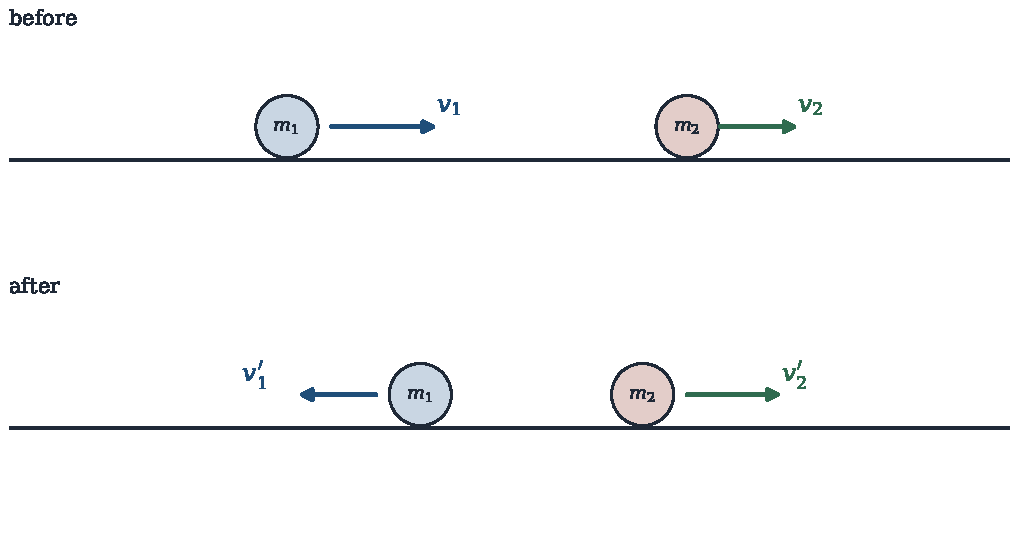
\includegraphics[width=0.72\textwidth]{figures/21_collision.pdf}
\caption{Two-particle collision in the laboratory frame. Total linear momentum $\vec{P}_{\text{tot}} = m_1\vec{v}_1 + m_2\vec{v}_2$ is conserved during the collision.}
\label{fig:collision}
\end{figure}

\section{Classification of Collisions in 1D}

In a brief collision between two bodies ($m_1, m_2$), the impact forces are so enormous that external forces (such as gravity or friction) are negligible during the collision duration $\Delta t \to 0$ (\textbf{impulsive approximation}).
Total momentum is always conserved:
\[
m_1 v_{1i} + m_2 v_{2i} = m_1 v_{1f} + m_2 v_{2f}.
\]
The elasticity of the collision is characterized by Newton's \textbf{coefficient of restitution} $e$:
\[
\boxed{e = -\frac{v_{1f} - v_{2f}}{v_{1i} - v_{2i}} = \frac{v_{\text{rel, final}}}{v_{\text{rel, initial}}} \in [0, 1].}
\]

\begin{center}
\renewcommand{\arraystretch}{1.3}
\begin{tabular}{@{}llll@{}}
\toprule
\textbf{Collision Type} & \textbf{Restitution $e$} & \textbf{Kinetic Energy $\Delta E_c$} & \textbf{Outcome} \\
\midrule
\textbf{Perfectly Elastic} & $e = 1$ & $\Delta E_c = 0$ (conserved) & $v_{1f} - v_{2f} = -(v_{1i} - v_{2i})$ \\
\textbf{Inelastic} & $0 < e < 1$ & $\Delta E_c < 0$ (partially lost) & Bodies bounce apart with reduced relative speed \\
\textbf{Perfectly Inelastic} & $e = 0$ & Maximum energy loss & Bodies stick together: $v_{1f} = v_{2f} = v_G$ \\
\bottomrule
\end{tabular}
\end{center}

For a 1D collision with known $e$, the final velocities are uniquely determined:
\[
\boxed{v_{1f} = v_G - \frac{m_2}{m_1 + m_2}e(v_{1i} - v_{2i}), \qquad v_{2f} = v_G + \frac{m_1}{m_1 + m_2}e(v_{1i} - v_{2i}).}
\]

\section{Center-of-Mass Frame and Koenig's First Theorem}

Let $\mathcal{R}^*$ be the center-of-mass frame (translating with velocity $\vec{v}_G$).
In this frame, the total linear momentum is identically zero: $\vec{P}^* = \vzero$.
The velocities in the laboratory and CM frames are related by $\vec{v}_i = \vec{v}_G + \vec{v}_i^*$.
The total kinetic energy in the laboratory frame satisfies \textbf{Koenig's First Theorem}:
\[
\boxed{E_c = \frac{1}{2}M v_G^2 + E_c^*,}
\]
where for a two-body system, the internal kinetic energy in the CM frame simplifies to:
\[
\boxed{E_c^* = \frac{1}{2}\mu\,v_{\text{rel}}^2, \quad \text{with reduced mass } \mu = \frac{m_1 m_2}{m_1 + m_2}.}
\]
In a collision, the kinetic energy of the center of mass $\frac{1}{2}M v_G^2$ can never be lost because $\vec{v}_G$ is constant!
The maximum possible kinetic energy that can be converted into heat/deformation (in a totally inelastic collision) is precisely $E_c^* = \frac{1}{2}\mu v_{\text{rel}}^2$.

\section{Worked Examples}

\begin{worked}[The ballistic pendulum]
A wooden block of mass $M = 1.98\ \mathrm{kg}$ hangs from light strings of length $L = 1.50\ \mathrm{m}$. A bullet of mass $m = 20.0\ \mathrm{g} = 0.0200\ \mathrm{kg}$ is fired horizontally into the block and embeds itself inside it. After impact, the block and bullet swing upward together to a maximum height $h = 8.50\ \mathrm{cm} = 0.0850\ \mathrm{m}$.
Find the initial speed $v_0$ of the bullet and the mechanical energy lost in the collision.
\end{worked}

\begin{solution}{16.1}
The problem consists of two distinct stages:
\begin{enumerate}[leftmargin=1.5em,itemsep=2pt]
  \item \textbf{Stage 1: Inelastic impact (duration $\Delta t \to 0$)}.
  External forces (gravity and string tension) do not have time to act horizontally. Total horizontal momentum is conserved:
  \[
  m v_0 = (M + m) V \implies V = \frac{m}{M + m}v_0,
  \]
  where $V$ is the speed of the combined mass immediately after impact.
  \item \textbf{Stage 2: Conservative upward swing}.
  After the collision, the tension in the strings does no work ($\vec{T}\perp\vec{v}$), and only gravity acts. Mechanical energy is conserved:
  \[
  \frac{1}{2}(M + m)V^2 = (M + m)gh \implies V = \sqrt{2gh}.
  \]
\end{enumerate}
Equating the two expressions for $V$:
\[
\frac{m}{M + m}v_0 = \sqrt{2gh} \implies \boxed{v_0 = \frac{M + m}{m}\sqrt{2gh}.}
\]
Computing numerically:
\[
\sqrt{2gh} = \sqrt{2(9.81)(0.0850)} = \sqrt{1.6677} \approx 1.291\ \mathrm{m\,s^{-1}}.
\]
Mass ratio: $\frac{M + m}{m} = \frac{1.98 + 0.0200}{0.0200} = \frac{2.00}{0.0200} = 100$.
The initial bullet speed is:
\[
v_0 = 100\times 1.291 = \mathbf{129.1\ \mathrm{m\,s^{-1}}.}
\]
Energy loss:
\begin{align*}
E_{c,\text{initial}} &= \frac{1}{2}m v_0^2 = \frac{1}{2}(0.0200)(129.1)^2 \approx 166.7\ \mathrm{J}, \\
E_{c,\text{after impact}} &= \frac{1}{2}(M + m)V^2 = \frac{1}{2}(2.00)(1.291)^2 \approx 1.67\ \mathrm{J}.
\end{align*}
The fraction of energy retained is only $\frac{m}{M+m} = \frac{1}{100} = 1\%$.
The mechanical energy lost is $\Delta E = 166.7 - 1.67 = \mathbf{165.0\ \mathrm{J}}$ ($99\%$ converted into heat, sound, and plastic deformation of the wood).
\end{solution}

\begin{worked}[Glancing 2D elastic collision of equal masses]
In a nuclear physics experiment, a proton of mass $m$ moving with speed $v_0$ collides elastically with another proton of equal mass $m$ initially at rest.
Prove that after the collision, the two protons always fly apart at a right angle ($90^\circ$), provided the collision is not head-on.
\end{worked}

\begin{solution}{16.2}
Let $\vec{v}_1$ and $\vec{v}_2$ be the final velocity vectors of the two protons after the collision.
\begin{itemize}[leftmargin=1.4em,itemsep=2pt]
  \item Conservation of linear momentum:
        \[
        m\vec{v}_0 = m\vec{v}_1 + m\vec{v}_2 \implies \vec{v}_0 = \vec{v}_1 + \vec{v}_2.
        \]
  \item Conservation of kinetic energy (elastic collision):
        \[
        \frac{1}{2}m v_0^2 = \frac{1}{2}m v_1^2 + \frac{1}{2}m v_2^2 \implies v_0^2 = v_1^2 + v_2^2.
        \]
\end{itemize}
Now take the dot product of the momentum vector equation with itself:
\[
\vec{v}_0\cdot\vec{v}_0 = (\vec{v}_1 + \vec{v}_2)\cdot(\vec{v}_1 + \vec{v}_2) \implies v_0^2 = v_1^2 + v_2^2 + 2\,\vec{v}_1\cdot\vec{v}_2.
\]
Subtracting the energy conservation equation ($v_0^2 = v_1^2 + v_2^2$):
\[
0 = 2\,\vec{v}_1\cdot\vec{v}_2 \implies \boxed{\vec{v}_1\cdot\vec{v}_2 = 0.}
\]
Since neither proton is at rest ($\vec{v}_1\ne\vzero, \vec{v}_2\ne\vzero$), their final velocity vectors are strictly orthogonal:
\[
\theta_1 + \theta_2 = \mathbf{90.0^\circ.}
\]
This iconic result is routinely observed in bubble chamber and cloud chamber photographs of proton-proton collisions.
\end{solution}

\section{Exercises and Step-by-Step Solutions}

\begin{exercise}{\warm\ Center of mass of a three-particle system}
Three masses lie in the $xy$-plane: $m_1 = 1.00\ \mathrm{kg}$ at $(1.0, 2.0)\ \mathrm{m}$, $m_2 = 2.00\ \mathrm{kg}$ at $(4.0, 1.0)\ \mathrm{m}$, and $m_3 = 3.00\ \mathrm{kg}$ at $(2.0, 5.0)\ \mathrm{m}$.
(a) Calculate the coordinates $(x_G, y_G)$ of the center of mass.
(b) If particle $m_1$ moves with velocity $\vec{v}_1 = 6.0\,\ihat\ \mathrm{m\,s^{-1}}$ while $m_2$ and $m_3$ are stationary, find the velocity $\vec{v}_G$ of the center of mass.
\end{exercise}

\begin{tabletworkspace}[5.0cm]
\end{tabletworkspace}

\begin{solution}{16.1}
(a) Total mass: $M = m_1 + m_2 + m_3 = 1.00 + 2.00 + 3.00 = 6.00\ \mathrm{kg}$.
Center of mass coordinates:
\begin{align*}
x_G &= \frac{m_1 x_1 + m_2 x_2 + m_3 x_3}{M} = \frac{1.00(1.0) + 2.00(4.0) + 3.00(2.0)}{6.00} = \frac{1.0 + 8.0 + 6.0}{6.00} = \frac{15.0}{6.00} = \mathbf{2.50\ \mathrm{m}.} \\
y_G &= \frac{m_1 y_1 + m_2 y_2 + m_3 y_3}{M} = \frac{1.00(2.0) + 2.00(1.0) + 3.00(5.0)}{6.00} = \frac{2.0 + 2.0 + 15.0}{6.00} = \frac{19.0}{6.00} \approx \mathbf{3.17\ \mathrm{m}.}
\end{align*}
Thus $\vec{r}_G = 2.50\,\ihat + 3.17\,\jhat\ \mathrm{m}$.

(b) Total linear momentum:
\[
\vec{P}_{\text{tot}} = m_1\vec{v}_1 + m_2\vec{v}_2 + m_3\vec{v}_3 = (1.00)(6.0\,\ihat) + \vzero + \vzero = 6.0\,\ihat\ \mathrm{kg\,m\,s^{-1}}.
\]
The center of mass velocity is:
\[
\vec{v}_G = \frac{\vec{P}_{\text{tot}}}{M} = \frac{6.0\,\ihat}{6.00} = \mathbf{1.00\,\ihat\ \mathrm{m\,s^{-1}}.}
\]
\end{solution}

\begin{exercise}{\warm\ 1D elastic collision and neutron moderation}
In a nuclear reactor, fast fission neutrons of mass $m_1 \approx 1\ \mathrm{u}$ moving at initial speed $v_0$ must be slowed down by head-on elastic collisions with stationary moderator nuclei of mass $m_2$.
(a) For a head-on elastic collision with $m_2$ at rest, show that the final speed of the neutron is:
\[
v_{1f} = \frac{m_1 - m_2}{m_1 + m_2}v_0.
\]
(b) Show that the fraction of kinetic energy transferred to the moderator nucleus is:
\[
\frac{\Delta E_c}{E_{c0}} = \frac{4 m_1 m_2}{(m_1 + m_2)^2}.
\]
(c) Evaluate this energy transfer fraction for a collision with ordinary hydrogen ($m_2 = 1\ \mathrm{u}$), carbon ($m_2 = 12\ \mathrm{u}$), and lead ($m_2 = 207\ \mathrm{u}$). Explain why water is an excellent neutron moderator while heavy metals are ineffective.
\end{exercise}

\begin{tabletworkspace}[5.5cm]
\end{tabletworkspace}

\begin{solution}{16.2}
(a) For an elastic collision ($e = 1$) with $v_{2i} = 0$:
\[
\text{Momentum:}\quad m_1 v_0 = m_1 v_{1f} + m_2 v_{2f}, \qquad \text{Restitution:}\quad v_{2f} - v_{1f} = v_0 \implies v_{2f} = v_0 + v_{1f}.
\]
Substituting into the momentum equation:
\[
m_1 v_0 = m_1 v_{1f} + m_2(v_0 + v_{1f}) = (m_1 + m_2)v_{1f} + m_2 v_0.
\]
Rearranging:
\[
(m_1 - m_2)v_0 = (m_1 + m_2)v_{1f} \implies \boxed{v_{1f} = \frac{m_1 - m_2}{m_1 + m_2}v_0.}
\]

(b) The final kinetic energy of the neutron is:
\[
E_{c1,f} = \frac{1}{2}m_1 v_{1f}^2 = \frac{1}{2}m_1 v_0^2\left(\frac{m_1 - m_2}{m_1 + m_2}\right)^2 = E_{c0}\left(\frac{m_1 - m_2}{m_1 + m_2}\right)^2.
\]
The kinetic energy transferred to the moderator nucleus is:
\[
\frac{\Delta E_c}{E_{c0}} = 1 - \left(\frac{m_1 - m_2}{m_1 + m_2}\right)^2 = \frac{(m_1 + m_2)^2 - (m_1 - m_2)^2}{(m_1 + m_2)^2} = \boxed{\frac{4m_1 m_2}{(m_1 + m_2)^2}.}
\]

(c) Numerical evaluation:
\begin{itemize}[leftmargin=1.4em,itemsep=2pt]
  \item Hydrogen ($m_2 = 1\ \mathrm{u}$): $\frac{4(1)(1)}{(1+1)^2} = \frac{4}{4} = \mathbf{1.00 = 100\%.}$ In a head-on collision with a proton, the neutron transfers $100\%$ of its kinetic energy and stops completely!
  \item Carbon-12 ($m_2 = 12\ \mathrm{u}$): $\frac{4(1)(12)}{(1+12)^2} = \frac{48}{169} \approx \mathbf{0.284 = 28.4\%.}$
  \item Lead-207 ($m_2 = 207\ \mathrm{u}$): $\frac{4(1)(207)}{(1+207)^2} = \frac{828}{(208)^2} = \frac{828}{43264} \approx \mathbf{0.019 = 1.9\%.}$
\end{itemize}
Because hydrogen nuclei (protons) match the neutron mass almost exactly, water ($\mathrm{H_2O}$) slows down neutrons rapidly in very few collisions. Heavy nuclei like lead barely recoil, bouncing the neutron elastically with almost zero energy loss!
\end{solution}

\begin{exercise}{\core\ Bouncing ball with coefficient of restitution $e$}
A rubber ball is dropped from rest from an initial height $h_0$ onto a rigid horizontal floor. The collision has a constant coefficient of restitution $e \in (0, 1)$.
(a) Find the height $h_n$ reached after the $n$-th bounce.
(b) Find the time interval $t_n$ between the $(n-1)$-th bounce and the $n$-th bounce.
(c) Sum the infinite geometric series to compute the total time $T_{\text{total}}$ until the ball stops bouncing, and the total distance $D_{\text{total}}$ traveled.
\end{exercise}

\begin{tabletworkspace}[6.0cm]
\end{tabletworkspace}

\begin{solution}{16.3}
(a) The impact speed before the first bounce is $v_1 = \sqrt{2gh_0}$.
After rebound, its speed is $u_1 = e v_1$.
The height reached after the first rebound is $h_1 = \frac{u_1^2}{2g} = \frac{e^2 v_1^2}{2g} = e^2 h_0$.
By induction, after $n$ rebounds:
\[
\boxed{h_n = e^{2n}h_0.}
\]

(b) Time to fall from $h_0$ to the first bounce: $t_0 = \sqrt{\frac{2h_0}{g}}$.
For each subsequent bounce $n \ge 1$, the ball goes up to height $h_n$ and falls back down, so the time between bounces is:
\[
t_n = 2\sqrt{\frac{2h_n}{g}} = 2\sqrt{\frac{2(e^{2n}h_0)}{g}} = 2e^n\sqrt{\frac{2h_0}{g}} = 2e^n t_0.
\]

(c) Total time to stop bouncing:
\[
T_{\text{total}} = t_0 + \sum_{n=1}^\infty t_n = t_0 + 2t_0\sum_{n=1}^\infty e^n = t_0\left( 1 + 2\frac{e}{1 - e} \right) = t_0\left(\frac{1 - e + 2e}{1 - e}\right) = \boxed{\sqrt{\frac{2h_0}{g}}\left(\frac{1 + e}{1 - e}\right).}
\]
Remarkably, although the ball undergoes infinitely many bounces, the total time is \textbf{finite}!

Total distance traveled:
\[
D_{\text{total}} = h_0 + 2\sum_{n=1}^\infty h_n = h_0 + 2h_0\sum_{n=1}^\infty e^{2n} = h_0\left( 1 + \frac{2e^2}{1 - e^2} \right) = \boxed{h_0\left(\frac{1 + e^2}{1 - e^2}\right).}
\]
\end{solution}

\begin{exercise}{\core\ The Tsiolkovsky Rocket Equation}
A rocket of total initial mass $m_0$ in deep space (zero gravity and zero drag) accelerates by ejecting burned propellant backward at a constant speed $u_{\text{ex}}$ relative to the rocket.
(a) In an inertial frame where the rocket has velocity $v$, analyze the momentum balance between time $t$ and $t + \dd t$ when mass $-\dd m$ ($\dd m < 0$) is ejected at speed $v - u_{\text{ex}}$ to derive the differential equation:
\[
m\,\dd v = -u_{\text{ex}}\,\dd m.
\]
(b) Integrate this equation to derive the famous \textbf{Tsiolkovsky Rocket Equation}:
\[
\Delta v = v_f - v_0 = u_{\text{ex}}\ln\left(\frac{m_0}{m_f}\right).
\]
(c) A rocket has an exhaust velocity $u_{\text{ex}} = 3000\ \mathrm{m\,s^{-1}}$. What mass ratio $m_0/m_f$ is required to achieve Earth orbital velocity $\Delta v = 7.80\ \mathrm{km\,s^{-1}}$?
\end{exercise}

\begin{tabletworkspace}[5.5cm]
\end{tabletworkspace}

\begin{solution}{16.4}
(a) At time $t$: the rocket and remaining fuel have mass $m$ and velocity $v$.
The total momentum is:
\[
P(t) = mv.
\]
At time $t + \dd t$: fuel of mass $\dd m_{\text{fuel}} = -\dd m > 0$ has been expelled backward with velocity $v - u_{\text{ex}}$ relative to the inertial frame. The rocket has mass $m + \dd m$ and velocity $v + \dd v$.
The momentum is:
\[
P(t + \dd t) = (m + \dd m)(v + \dd v) + (-\dd m)(v - u_{\text{ex}}) = mv + m\,\dd v + v\,\dd m + \dd m\dd v - v\,\dd m + u_{\text{ex}}\,\dd m.
\]
Dropping the second-order differential $\dd m\dd v$:
\[
P(t + \dd t) = mv + m\,\dd v + u_{\text{ex}}\,\dd m.
\]
Since no external force acts ($F_{\text{ext}} = 0$):
\[
P(t + \dd t) - P(t) = 0 \implies m\,\dd v + u_{\text{ex}}\,\dd m = 0 \implies \boxed{m\,\dd v = -u_{\text{ex}}\,\dd m.}
\]

(b) Dividing by $m$:
\[
\dd v = -u_{\text{ex}}\frac{\dd m}{m}.
\]
Integrating from initial state $(m_0, v_0)$ to final empty propellant burnout state $(m_f, v_f)$:
\[
\int_{v_0}^{v_f} \dd v = -u_{\text{ex}}\int_{m_0}^{m_f} \frac{\dd m}{m} \implies v_f - v_0 = -u_{\text{ex}}\left[ \ln m_f - \ln m_0 \right].
\]
Using $\ln(m_f/m_0) = -\ln(m_0/m_f)$:
\[
\boxed{\Delta v = u_{\text{ex}}\ln\left(\frac{m_0}{m_f}\right).}
\]

(c) Given $\Delta v = 7800\ \mathrm{m\,s^{-1}}$ and $u_{\text{ex}} = 3000\ \mathrm{m\,s^{-1}}$:
\[
\ln\left(\frac{m_0}{m_f}\right) = \frac{\Delta v}{u_{\text{ex}}} = \frac{7800}{3000} = 2.60.
\]
Taking the exponential:
\[
\frac{m_0}{m_f} = e^{2.60} \approx \mathbf{13.46.}
\]
This means the fuel must constitute $\frac{13.46 - 1}{13.46} \approx \mathbf{92.6\%}$ of the rocket's total launch mass! This exponential dependence explains why multi-stage rockets are essential for space exploration.
\end{solution}

\begin{exercise}{\mastery\ Synoptic Problem: The Spring Launcher and Vertical Loop}
A block of mass $m=0.500\ \mathrm{kg}$ is pushed against a horizontal spring of stiffness $k=800\ \mathrm{N\,m^{-1}}$, compressing it by $\Delta x = 0.200\ \mathrm{m}$.
Upon release, the block moves along a smooth horizontal track, crosses a rough horizontal patch of length $d=0.800\ \mathrm{m}$ with kinetic friction coefficient $\mu_k = 0.250$, and then enters a smooth vertical circular loop of radius $R = 0.500\ \mathrm{m}$.
(a) Find the speed $v_1$ of the block immediately after separating from the spring.
(b) Find the speed $v_2$ after traversing the rough patch.
(c) Determine whether the block completes the loop without falling off, and calculate the normal reaction force $N_{\text{top}}$ at the very top of the loop.
\end{exercise}

\begin{tabletworkspace}[6.5cm]
\end{tabletworkspace}

\begin{solution}{16.5}
(a) From release to spring separation: only the conservative spring force acts.
Mechanical energy conservation:
\[
E_{m0} = \frac{1}{2}k(\Delta x)^2 = \frac{1}{2}m v_1^2 \implies v_1 = \Delta x\sqrt{\frac{k}{m}}.
\]
Computing:
\[
v_1 = 0.200\sqrt{\frac{800}{0.500}} = 0.200\sqrt{1600} = 0.200\times 40.0 = \mathbf{8.00\ \mathrm{m\,s^{-1}}.}
\]

(b) Across the rough patch of length $d$: friction does work $W_f = -\mu_k mg d$.
Work-energy theorem:
\[
\frac{1}{2}m v_2^2 - \frac{1}{2}m v_1^2 = -\mu_k mg d \implies v_2^2 = v_1^2 - 2\mu_k gd.
\]
Computing:
\[
v_2^2 = (8.00)^2 - 2(0.250)(9.81)(0.800) = 64.0 - 3.924 = 60.076\ \mathrm{m^2\,s^{-2}}.
\]
\[
v_2 = \sqrt{60.076} \approx \mathbf{7.75\ \mathrm{m\,s^{-1}}.}
\]

(c) In the smooth vertical loop: only gravity performs work as the block rises to height $2R = 2(0.500) = 1.00\ \mathrm{m}$.
Work-energy theorem to the top of the loop:
\[
\frac{1}{2}m v_{\text{top}}^2 - \frac{1}{2}m v_2^2 = -mg(2R) \implies v_{\text{top}}^2 = v_2^2 - 4gR.
\]
Computing:
\[
v_{\text{top}}^2 = 60.076 - 4(9.81)(0.500) = 60.076 - 19.62 = 40.456\ \mathrm{m^2\,s^{-2}} \implies v_{\text{top}} \approx 6.36\ \mathrm{m\,s^{-1}}.
\]
The condition to complete the loop without leaving the track is $v_{\text{top}}^2 \ge gR$:
\[
gR = 9.81\times 0.500 = 4.905\ \mathrm{m^2\,s^{-2}}.
\]
Since $v_{\text{top}}^2 = 40.46 \gg 4.91$, the block \textbf{comfortably completes the loop}!
The normal force at the top is:
\[
N_{\text{top}} = m\frac{v_{\text{top}}^2}{R} - mg = \frac{0.500\times 40.456}{0.500} - 0.500(9.81) = 40.456 - 4.905 \approx \mathbf{35.55\ \mathrm{N}.}
\]
\end{solution}

\begin{exercise}{\mastery\ Synoptic Problem: Gravitational Slingshot (Planetary Flyby)}
A spacecraft of mass $m$ approaches Jupiter (mass $M \gg m$) which orbits the Sun at speed $V_J = 13.0\ \mathrm{km\,s^{-1}}$. In the solar frame, the spacecraft moves with speed $v_0 = 10.0\ \mathrm{km\,s^{-1}}$ directly toward Jupiter (head-on encounter).
(a) Using a Galilean transformation, find the velocity $u_i$ of the spacecraft in Jupiter's rest frame before the encounter.
(b) Since gravitational deflection is an elastic scattering in Jupiter's rest frame, the spacecraft swings around Jupiter and emerges traveling in the opposite direction. What is its speed $u_f$ in Jupiter's frame?
(c) Transform back to the solar frame to find the final speed $v_f$ of the spacecraft. How much kinetic energy did the spacecraft gain from Jupiter's orbital motion?
\end{exercise}

\begin{tabletworkspace}[6.0cm]
\end{tabletworkspace}

\begin{solution}{16.6}
(a) Choose the $x$-axis in the direction of Jupiter's orbital motion: $\vec{V}_J = +V_J\ihat = +13.0\,\ihat\ \mathrm{km\,s^{-1}}$.
The incoming spacecraft travels toward Jupiter in head-on approach: $\vec{v}_0 = -v_0\ihat = -10.0\,\ihat\ \mathrm{km\,s^{-1}}$.
In Jupiter's reference frame $\mathcal{R}_J$, the relative velocity is:
\[
\vec{u}_i = \vec{v}_0 - \vec{V}_J = -10.0\,\ihat - 13.0\,\ihat = \mathbf{-23.0\,\ihat\ \mathrm{km\,s^{-1}}.}
\]
The spacecraft approaches Jupiter at speed $u_i = 23.0\ \mathrm{km\,s^{-1}}$.

(b) In Jupiter's frame, the spacecraft moves in a conservative gravitational hyperbola. By conservation of energy in $\mathcal{R}_J$, the outgoing asymptotic speed equals the incoming asymptotic speed:
\[
u_f = u_i = 23.0\ \mathrm{km\,s^{-1}}.
\]
After completing a $180^\circ$ swing around the planet, its outgoing velocity in Jupiter's frame is reversed:
\[
\vec{u}_f = +u_i\ihat = \mathbf{+23.0\,\ihat\ \mathrm{km\,s^{-1}}.}
\]

(c) Transforming back to the Sun's inertial frame:
\[
\vec{v}_f = \vec{u}_f + \vec{V}_J = +23.0\,\ihat + 13.0\,\ihat = \mathbf{+36.0\,\ihat\ \mathrm{km\,s^{-1}}.}
\]
The final speed is:
\[
\boxed{v_f = v_0 + 2V_J = 10.0 + 2(13.0) = \mathbf{36.0\ \mathrm{km\,s^{-1}}!}}
\]
The spacecraft has gained $\Delta v = 26.0\ \mathrm{km\,s^{-1}}$!
Kinetic energy change per unit mass:
\[
\Delta\left(\frac{E_c}{m}\right) = \frac{1}{2}v_f^2 - \frac{1}{2}v_0^2 = \frac{1}{2}(36.0^2 - 10.0^2) = \frac{1}{2}(1296 - 100) = \mathbf{598\ \mathrm{MJ\,kg^{-1}}.}
\]
This tremendous energy boost is taken directly from Jupiter's enormous orbital kinetic energy around the Sun (slowing Jupiter down by an utterly imperceptible $\Delta V_J \sim 10^{-21}\ \mathrm{m\,s^{-1}}$). This is the gravity assist technique used by the Voyager, Cassini, and New Horizons probes!
\end{solution}


\appendix
\part*{Appendices}
\addcontentsline{toc}{part}{Appendices}
\chapter{Mathematical Reference Toolbox}
\label{app:math}

\section{Coordinate Systems and Unit Vectors}

\subsection{Cartesian Coordinates $(x, y, z)$}
\begin{itemize}[leftmargin=1.4em,itemsep=2pt]
  \item Position vector: $\vec{r} = x\ihat + y\jhat + z\khat$
  \item Displacement: $\dd\vec{r} = \dd x\ihat + \dd y\jhat + \dd z\khat$
  \item Velocity: $\vec{v} = \dot{x}\ihat + \dot{y}\jhat + \dot{z}\khat$
  \item Acceleration: $\vec{a} = \ddot{x}\ihat + \ddot{y}\jhat + \ddot{z}\khat$
\end{itemize}

\subsection{Plane Polar Coordinates $(r, \theta)$}
\begin{itemize}[leftmargin=1.4em,itemsep=2pt]
  \item Relation to Cartesian: $x = r\cos\theta, \quad y = r\sin\theta$
  \item Basis vectors: $\ur = \cos\theta\ihat + \sin\theta\jhat, \quad \ut = -\sin\theta\ihat + \cos\theta\jhat$
  \item Derivatives of basis vectors: $\frac{\dd\ur}{\dd t} = \dot{\theta}\ut, \quad \frac{\dd\ut}{\dd t} = -\dot{\theta}\ur$
  \item Position vector: $\vec{r} = r\ur$
  \item Displacement: $\dd\vec{r} = \dd r\ur + r\dd\theta\ut$
  \item Velocity: $\vec{v} = \dot{r}\ur + r\dot{\theta}\ut$
  \item Acceleration: $\vec{a} = (\ddot{r} - r\dot{\theta}^2)\ur + (r\ddot{\theta} + 2\dot{r}\dot{\theta})\ut = (\ddot{r} - r\dot{\theta}^2)\ur + \frac{1}{r}\frac{\dd(r^2\dot{\theta})}{\dd t}\ut$
\end{itemize}

\subsection{Cylindrical Coordinates $(\rho, \theta, z)$}
\begin{itemize}[leftmargin=1.4em,itemsep=2pt]
  \item Position vector: $\vec{r} = \rho\vec{u}_\rho + z\khat$
  \item Velocity: $\vec{v} = \dot{\rho}\vec{u}_\rho + \rho\dot{\theta}\ut + \dot{z}\khat$
  \item Acceleration: $\vec{a} = (\ddot{\rho} - \rho\dot{\theta}^2)\vec{u}_\rho + (\rho\ddot{\theta} + 2\dot{\rho}\dot{\theta})\ut + \ddot{z}\khat$
\end{itemize}

\subsection{Spherical Coordinates $(r, \theta, \phi)$}
\begin{itemize}[leftmargin=1.4em,itemsep=2pt]
  \item Relation to Cartesian: $x = r\sin\theta\cos\phi, \quad y = r\sin\theta\sin\phi, \quad z = r\cos\theta$
  \item Position vector: $\vec{r} = r\ur$
  \item Velocity: $\vec{v} = \dot{r}\ur + r\dot{\theta}\ut + r\sin\theta\dot{\phi}\uphi$
  \item Acceleration:
  \begin{align*}
  a_r &= \ddot{r} - r\dot{\theta}^2 - r\sin^2\theta\dot{\phi}^2, \\
  a_\theta &= r\ddot{\theta} + 2\dot{r}\dot{\theta} - r\sin\theta\cos\theta\dot{\phi}^2, \\
  a_\phi &= r\sin\theta\ddot{\phi} + 2\sin\theta\dot{r}\dot{\phi} + 2r\cos\theta\dot{\theta}\dot{\phi}.
  \end{align*}
\end{itemize}

\subsection{Intrinsic Coordinates (Frenet-Serret Frame)}
\begin{itemize}[leftmargin=1.4em,itemsep=2pt]
  \item Basis: $\utt$ (tangent), $\un$ (principal normal directed toward center of curvature), $\vec{u}_b = \utt\times\un$ (binormal)
  \item Velocity: $\vec{v} = v\,\utt$ with $v = \frac{\dd s}{\dd t}$
  \item Acceleration: $\vec{a} = a_t\,\utt + a_n\,\un = \frac{\dd v}{\dd t}\utt + \frac{v^2}{R}\un$
  where $R$ is the local radius of curvature ($R = \frac{\dd s}{\dd\phi}$).
\end{itemize}

\section{Vector Differential Identities}

For scalar fields $f, g$ and vector fields $\vec{A}, \vec{B}$:
\begin{itemize}[leftmargin=1.4em,itemsep=2pt]
  \item $\vec{\nabla}(fg) = f\vec{\nabla} g + g\vec{\nabla} f$
  \item $\vec{\nabla}\cdot(f\vec{A}) = f(\vec{\nabla}\cdot\vec{A}) + \vec{A}\cdot\vec{\nabla} f$
  \item $\vec{\nabla}\times(f\vec{A}) = f(\vec{\nabla}\times\vec{A}) + (\vec{\nabla} f)\times\vec{A}$
  \item $\vec{\nabla}\times(\vec{\nabla} f) = \vzero$ \quad (\textbf{every gradient field is irrotational / conservative})
  \item $\vec{\nabla}\cdot(\vec{\nabla}\times\vec{A}) = 0$ \quad (\textbf{every curl field is divergence-free})
  \item $\vec{\nabla}\times(\vec{\nabla}\times\vec{A}) = \vec{\nabla}(\vec{\nabla}\cdot\vec{A}) - \Delta\vec{A}$
\end{itemize}

\section{Essential Taylor Series Approximations ($x \to 0$)}

\begin{align*}
(1 + x)^n &= 1 + nx + \frac{n(n-1)}{2}x^2 + \dots \\
\sqrt{1 + x} &= 1 + \frac{1}{2}x - \frac{1}{8}x^2 + \dots \\
\frac{1}{1 + x} &= 1 - x + x^2 - x^3 + \dots \\
\frac{1}{\sqrt{1 + x}} &= 1 - \frac{1}{2}x + \frac{3}{8}x^2 + \dots \\
e^x &= 1 + x + \frac{1}{2}x^2 + \frac{1}{6}x^3 + \dots \\
\ln(1 + x) &= x - \frac{1}{2}x^2 + \frac{1}{3}x^3 + \dots \\
\sin x &= x - \frac{1}{6}x^3 + \dots \\
\cos x &= 1 - \frac{1}{2}x^2 + \frac{1}{24}x^4 + \dots \\
\tan x &= x + \frac{1}{3}x^3 + \dots
\end{align*}

\chapter{Physical Constants and Astronomical Data}
\label{app:constants}

\section{Fundamental Physical Constants}

\begin{center}
\renewcommand{\arraystretch}{1.3}
\begin{tabular}{@{}llll@{}}
\toprule
\textbf{Constant} & \textbf{Symbol} & \textbf{Standard Value} & \textbf{SI Units} \\
\midrule
Gravitational constant & $G$ & $6.67430(15)\times 10^{-11}$ & $\mathrm{m^3\,kg^{-1}\,s^{-2}} = \mathrm{N\,m^2\,kg^{-2}}$ \\
Speed of light in vacuum & $c$ & $299\,792\,458$ (exact) & $\mathrm{m\,s^{-1}}$ \\
Standard gravity near Earth & $g$ & $9.80665$ (exact standard) & $\mathrm{m\,s^{-2}} = \mathrm{N\,kg^{-1}}$ \\
Elementary charge & $e$ & $1.602176634\times 10^{-19}$ (exact) & $\mathrm{C}$ \\
Vacuum permittivity & $\varepsilon_0$ & $8.8541878128\times 10^{-12}$ & $\mathrm{F\,m^{-1}} = \mathrm{C^2\,N^{-1}\,m^{-2}}$ \\
Coulomb constant & $k_e = \frac{1}{4\pi\varepsilon_0}$ & $8.9875517923\times 10^9$ & $\mathrm{N\,m^2\,C^{-2}}$ \\
Planck constant & $h$ & $6.62607015\times 10^{-34}$ (exact) & $\mathrm{J\,s} = \mathrm{kg\,m^2\,s^{-1}}$ \\
Avogadro constant & $N_A$ & $6.02214076\times 10^{23}$ (exact) & $\mathrm{mol^{-1}}$ \\
Atomic mass unit & $1\ \mathrm{u}$ & $1.660539066\times 10^{-27}$ & $\mathrm{kg}$ \\
Electron mass & $m_e$ & $9.1093837\times 10^{-31}$ & $\mathrm{kg}$ \\
Proton mass & $m_p$ & $1.6726219\times 10^{-27}$ & $\mathrm{kg}$ \\
Neutron mass & $m_n$ & $1.6749275\times 10^{-27}$ & $\mathrm{kg}$ \\
\bottomrule
\end{tabular}
\end{center}

\section{Earth, Moon, and Solar Data}

\begin{center}
\renewcommand{\arraystretch}{1.3}
\begin{tabular}{@{}llll@{}}
\toprule
\textbf{Quantity} & \textbf{Symbol} & \textbf{Value} & \textbf{SI Units} \\
\midrule
Earth's mass & $M_E$ & $5.9722\times 10^{24}$ & $\mathrm{kg}$ \\
Earth's equatorial radius & $R_e$ & $6.3781\times 10^6$ & $\mathrm{m}$ \\
Earth's polar radius & $R_p$ & $6.3568\times 10^6$ & $\mathrm{m}$ \\
Earth's mean volumetric radius & $R_E$ & $6.3710\times 10^6$ & $\mathrm{m}$ \\
Earth's angular rotation rate & $\Omega_E$ & $7.292115\times 10^{-5}$ & $\mathrm{rad\,s^{-1}}$ \\
Earth's sidereal day & $T_{\text{sidereal}}$ & $86\,164.1$ ($23\ \mathrm{h}\ 56\ \mathrm{m}\ 4.1\ \mathrm{s}$) & $\mathrm{s}$ \\
Moon's mass & $M_M$ & $7.342\times 10^{22}$ & $\mathrm{kg}$ \\
Moon's mean radius & $R_M$ & $1.7374\times 10^6$ & $\mathrm{m}$ \\
Earth-Moon mean distance & $d_{EM}$ & $3.844\times 10^8$ & $\mathrm{m}$ \\
Sun's mass & $M_\odot$ & $1.9885\times 10^{30}$ & $\mathrm{kg}$ \\
Sun's radius & $R_\odot$ & $6.957\times 10^8$ & $\mathrm{m}$ \\
Astronomical Unit (mean Sun-Earth distance) & $1\ \mathrm{AU}$ & $1.495978707\times 10^{11}$ (exact) & $\mathrm{m}$ \\
Solar gravitational parameter & $\mu_\odot = GM_\odot$ & $1.3271244\times 10^{20}$ & $\mathrm{m^3\,s^{-2}}$ \\
Earth gravitational parameter & $\mu_E = GM_E$ & $3.9860044\times 10^{14}$ & $\mathrm{m^3\,s^{-2}}$ \\
\bottomrule
\end{tabular}
\end{center}

\chapter{Comprehensive Formula Sheet and Problem-Solving Protocols}
\label{app:formula_sheet}

\section{The Five-Step Mechanics Problem-Solving Protocol}

Whenever you encounter a mechanics problem, systematically follow this standard five-step algorithm:

\begin{enumerate}[leftmargin=1.8em,itemsep=4pt]
  \item \textbf{Define the System and the Reference Frame}:
        \begin{itemize}[leftmargin=1.4em,itemsep=2pt]
          \item Explicitly specify the particle(s) or body being studied.
          \item Choose an appropriate reference frame $\mathcal{R}$ (Galilean whenever possible; otherwise identify the non-inertial acceleration $\vec{a}_e$ and angular velocity $\vec{\Omega}$).
          \item Select the most natural coordinate system (Cartesian for uniform fields; Polar/Cylindrical for circular/axial symmetry; Spherical for central fields; Frenet for known trajectories).
        \end{itemize}
  \item \textbf{Perform the Comprehensive Force Inventory (Free-Body Diagram)}:
        \begin{itemize}[leftmargin=1.4em,itemsep=2pt]
          \item Field forces (at a distance): Weight $\vec{P} = m\vec{g}$, Gravitation $\vec{F}_g = -G\frac{Mm}{r^2}\ur$, Electrostatic $\vec{F}_e = q\vec{E}$.
          \item Contact forces: Normal reaction $\vec{N}$ (orthogonal to surface), Friction $\vec{f}$ (tangential, static $f_s \le \mu_s N$ or kinetic $f_k = \mu_k N$), Tension $\vec{T}$ (along string/rope), Spring restoring force $\vec{F}_s = -k(\ell - \ell_0)\vec{u}$.
          \item Fictitious forces (if in non-inertial frame): $\vec{F}_{ie} = -m\vec{a}_e$ and $\vec{F}_{ic} = -2m\vec{\Omega}\times\vec{v}_r$.
        \end{itemize}
  \item \textbf{Select the Optimal Fundamental Principle}:
        \begin{itemize}[leftmargin=1.4em,itemsep=2pt]
          \item If seeking accelerations or forces at an instant $\rightarrow$ \textbf{Newton's Second Law}: $\sum\vec{F} = m\vec{a}$.
          \item If relating speeds and positions without tracking time $\rightarrow$ \textbf{Work-Energy Theorem}: $\Delta E_c = W_{\text{all forces}}$ or \textbf{Conservation of Mechanical Energy}: $\Delta E_m = W_{\text{nc}}$.
          \item If dealing with rotational, central, or orbital motion $\rightarrow$ \textbf{Angular Momentum Theorem}: $\frac{\dd\vec{L}_O}{\dd t} = \vec{\tau}_O$.
          \item If dealing with sudden collisions, impacts, or explosions $\rightarrow$ \textbf{Conservation of Linear Momentum}: $\vec{P}_{\text{tot}} = \text{const}$.
        \end{itemize}
  \item \textbf{Project and Integrate}:
        \begin{itemize}[leftmargin=1.4em,itemsep=2pt]
          \item Project the vector equation onto the coordinate axes.
          \item Separate variables and integrate with respect to time or space using initial conditions.
        \end{itemize}
  \item \textbf{Sanity Checks}:
        \begin{itemize}[leftmargin=1.4em,itemsep=2pt]
          \item \textbf{Dimensional check}: Verify that both sides have the same physical units!
          \item \textbf{Limiting cases}: Check limits (e.g. $\theta \to 0$, $m_1 \gg m_2$, friction $\mu \to 0$, $t \to \infty$).
          \item \textbf{Physical plausibility}: Is the sign reasonable? Is the numerical order of magnitude realistic?
        \end{itemize}
\end{enumerate}

\section{Core Formula Quick-Reference Sheet}

\subsection{Kinematics}
\begin{align*}
\text{1D Constant Acceleration:}\quad & v(t) = at + v_0, \quad x(t) = \tfrac{1}{2}at^2 + v_0 t + x_0, \quad v^2 - v_0^2 = 2a(x - x_0) \\
\text{Frenet Frame:}\quad & \vec{v} = v\,\utt, \quad \vec{a} = \dot{v}\,\utt + \frac{v^2}{R}\un \\
\text{Polar Coordinates:}\quad & \vec{v} = \dot{r}\ur + r\dot{\theta}\ut, \quad \vec{a} = (\ddot{r} - r\dot{\theta}^2)\ur + (r\ddot{\theta} + 2\dot{r}\dot{\theta})\ut \\
\text{Composition of Velocities:}\quad & \vec{v}_a = \vec{v}_r + \vec{v}_e \quad (\vec{v}_e = \vec{v}(O') + \vec{\Omega}\times\vec{r}') \\
\text{Composition of Accelerations:}\quad & \vec{a}_a = \vec{a}_r + \vec{a}_e + \vec{a}_c \quad (\vec{a}_c = 2\vec{\Omega}\times\vec{v}_r)
\end{align*}

\subsection{Dynamics and Forces}
\begin{align*}
\text{Newton's 2nd Law (Inertial):}\quad & \sum\vec{F} = m\vec{a} = \frac{\dd\vec{p}}{\dd t} \\
\text{Newton's 2nd Law (Non-Inertial):}\quad & m\vec{a}_r = \sum\vec{F}_{\text{real}} - m\vec{a}_e - 2m\,\vec{\Omega}\times\vec{v}_r \\
\text{Coulomb Solid Friction:}\quad & \text{Static: } f_s \le \mu_s N, \quad \text{Kinetic: } f_k = \mu_k N \\
\text{Hooke's Law:}\quad & \vec{F}_s = -k(x - x_0)\ihat
\end{align*}

\subsection{Work, Energy, and Oscillations}
\begin{align*}
\text{Work-Energy Theorem:}\quad & \Delta E_c = W_{A\to B}(\sum\vec{F}) \\
\text{Conservative Force:}\quad & \vec{F} = -\vec{\nabla} E_p \iff \vec{\nabla}\times\vec{F} = \vzero \\
\text{Total Mechanical Energy:}\quad & E_m = E_c + E_p, \quad \frac{\dd E_m}{\dd t} = P_{\text{nc}} = \vec{F}_{\text{nc}}\cdot\vec{v} \\
\text{Small Oscillations around } x_0:\quad & \omega_0 = \sqrt{\frac{k_{\text{eff}}}{m}}, \quad k_{\text{eff}} = \left.\frac{\dd^2 E_p}{\dd x^2}\right|_{x_0} > 0 \\
\text{Damped Oscillator:}\quad & \ddot{x} + 2\lambda\dot{x} + \omega_0^2 x = 0, \quad \omega_d = \sqrt{\omega_0^2 - \lambda^2}, \quad Q = \frac{\omega_0}{2\lambda}
\end{align*}

\subsection{Angular Momentum and Central Forces}
\begin{align*}
\text{Angular Momentum Theorem:}\quad & \frac{\dd\vec{L}_O}{\dd t} = \vec{\tau}_O = \vec{r}\times\vec{F} \\
\text{Central Force Conservation:}\quad & \vec{L}_O = \text{const} \implies r^2\dot{\theta} = C = \text{const} \\
\text{Effective Potential:}\quad & U_{\text{eff}}(r) = U(r) + \frac{L^2}{2mr^2} \\
\text{Vis-Viva Equation (Kepler):}\quad & v^2 = GM\left(\frac{2}{r} - \frac{1}{a}\right), \quad T^2 = \frac{4\pi^2}{GM}a^3
\end{align*}

\subsection{Systems and Collisions}
\begin{align*}
\text{Center of Mass:}\quad & M\vec{a}_G = \sum\vec{F}_{\text{ext}} \\
\text{1D Restitution Coefficient:}\quad & e = -\frac{v_{1f} - v_{2f}}{v_{1i} - v_{2i}} \in [0, 1] \\
\text{Koenig's First Theorem:}\quad & E_c = \frac{1}{2}M v_G^2 + \frac{1}{2}\mu v_{\text{rel}}^2, \quad \mu = \frac{m_1 m_2}{m_1 + m_2} \\
\text{Tsiolkovsky Rocket:}\quad & \Delta v = u_{\text{ex}}\ln\left(\frac{m_0}{m_f}\right)
\end{align*}


\end{document}
